% ======================================================= %
%          Phd Thesis of Isis Van Parijs             %
%                                                         %
%  Structure:                                             %
%   template.tex          (main file)                     %
%    - _packages.tex      (load packages)                 %
%    - _settings.tex      (basic configuration)           %
%    - _newcommands.tex   (custom commands)               %
%    - 1 - Introduction/  (chapters in subdirectories)    %
%    - 2 - ...                                            %
%    -                                                    %
%                                                         %
% ======================================================= %

% draft or final?
\newcommand{\status}{final} % balck lines next to overfull boxes
% If the draft option is passed to the package, all micro-typographic extensions will be disabled, which may lead to different line, and hence page, breaks. The draft and final options may also be inherited from the class options; of course, you can override them in the package options. E. g., if you are using the class option draft to show any overfull boxes, you should load microtype with the final option.

% The most general information for this document
\newcommand{\Title}{A search for flavour changing neutral currents involving a top quark and a Z boson, using the data collected by the CMS experiment at a centre-of-mass energy of 13 TeV}
\newcommand{\Titledutch}{``Een zoektocht naar smaakveranderende neutrale stromen gerelateerd met een top quark en een Z boson, gebruik makend van de data gecollecteerd door het CMS experiment met een massamiddelpuntsenergie van 13 TeV.''}
\newcommand{\Pdftitle}{\Title}  % For if you want to have a different title in the pdf document (e.g. special characters removed)
\newcommand{\Author}{Isis Van Parijs}
\newcommand{\keywords}{LaTeX, template, CMS, FCNC, phd, thesis}
\newcommand{\refereeOne}{Prof.~Dr.~J. D'Hondt}
%\newcommand{\refereeTwo}{Prof.~Dr.~P. Thagoras}
\newcommand{\dateHandIn}{17~December~2017}
\newcommand{\dateDefense}{17~January~2018}


% load the general configuration
%!TEX root = template.tex

% -- packages -------------------------------------- %

% basic layout of the document
\documentclass[
  11pt, a4paper,        % font and paper size
  fleqn,                % align equations to the left
  twoside, openright,   % two sided option with new chapters on the right page
  \status               % the status (defined in main document)
]{memoir}

% general stuff
\usepackage[utf8]{inputenc}   % Input-Encoding
                              % (encoding which is used for saving)
\usepackage[TS1,T1]{fontenc}  % Output-Encoding
                              % (Latin1 [T1] with additional sepecial characters [TS1])

% \usepackage[ngerman]{babel}   % German language package
\usepackage[english]{babel}   % English language package

% image stuff
\usepackage[final]{graphicx}  % include graphics
\usepackage{rotating}         % rotate images
% \usepackage{caption}          % customize your captions (memoir incompatible)
% \usepackage{subfig}           % sub-captions (memoir incompatible, already included there with \subbottom)
\usepackage{wrapfig}          % wrap text around images and tables
\usepackage{afterpage}
\usepackage{lscape}

% font and symbols
\usepackage[charter, greeklowercase=upright]{mathdesign} % Bitstream Charter font, not-italic greek letter like \alphaup
\usepackage[scaled=.96,lining]{XCharter} % Provides additional Charter-like symbols, and small caps
\usepackage{microtype}        % better type setting
% \usepackage{amssymb,amsmath}  % more math symbols and environments % mathdesign interferes with amssymb
% \usepackage{textcomp}         % even more special characters
\usepackage{tikz}             % used to make circled numbers
\usepackage{color}            % define your own colors
\usepackage{scrhack}          % fixes an error caused by listings package
\usepackage{listings}         % enables syntax highlighting for your code
\usepackage{zi4}              % Use Inconsolata for fixed-width texttt

%quotes
%\usepackage{quotchap}

% references
\usepackage[backend=biber,style=numeric-comp]{biblatex}
%\usepackage{cite}
% physics and maths
\usepackage{amsmath}
\usepackage{wasysym}          % glyphs and other symbols, e.g. \int, http://www.ctan.org/pkg/wasysym
\usepackage[alsoload=hep]{siunitx}          % macros for printing numbers (\num{12345}) and units (\SI{1e7}{\kilogram\per\metre\squared}), also interesting: \SIrange{10}{30}{\metre}, \mega\electronvolt, \DeclareSIUnit. \per can be set individually via SI[per-mode=reciprocal], or per-mode-fraction to overwrite the new default in the next line; http://www.ctan.org/pkg/siunitx
\usepackage{commath}          % defines differential operators (\del, \dif)
\usepackage{feynmp-auto}      % Feynman diagrams (alternative: feynmf)
\usepackage{cancel, slashed}  % Feynman notation
% \usepackage{maybemath}        % For context-sensitive maths, like headings
\usepackage{hepparticles}     % particle names
\usepackage{hepnames}         % shortcuts for lots of particle names
\usepackage{braket}           % provides \bra and \ket notation

% configuration
\usepackage{hyperref}         % hyperlinks in PDF
% The two following packages don't work with the memoir style
% \usepackage{fancyhdr}         % configure your page header
% \usepackage[noindentafter]{titlesec}  % configure titles

% table stuff
\usepackage{booktabs}         % professional tables
\usepackage{multirow}         % combine table rows
% \usepackage{arydshln}         % dashed lines in tables

% additional packages (mixed)
% \usepackage{keystroke}        % display keystrokes
\usepackage{xspace}           % adds spaces to the end of commands if needed
\usepackage{pdflscape}        % allows for landscaped, pdf-rotated single pages
\usepackage[acronym,nonumberlist,xindy]{glossaries-prefix}  % glossaries % xindy is used for sorting non-latin characters correctly
\usepackage{multicol}         % offers multi column environments
\usepackage{ifdraft}          % offers \ifdraft{}{} command to do stuff while in draft mode
% \usepackage{panda}            % Custom \panda package for overlining the P
% \usepackage{gitinfo2}         % Provides infos about git (needs hooks, though)

% packages that help during draft versions
% (change document option from draft to final to disable)
\usepackage[obeyDraft,textsize=scriptsize]
  {todonotes}                 % notes and missing images
% \usepackage{showlabels}       % show label names next to numbering

%!TEX root = template.tex

% configure the microtype font setting
\microtypesetup{
  final,        % always activate, even when in draft mode
  activate={true,nocompatibility},  % activate protrusion and expansion
  % tracking=true,  % This is disabled because it adds extra space around small caps. It's suppose to be disabled with \SetTracking{encoding={*}, shape=sc}{0}, but I can't verify this. Maybe you can figure it out!
  kerning=true,
  spacing=true,
  protrusion=true
  % more info on config to be found eg at http://www.khirevich.com/latex/microtype/
}
\microtypecontext{spacing=nonfrench}
% enable protrusion for superscript numbers
% (doesn't work with XeTeX right now)
% \SetProtrusion{
%   encoding={*},
%   family={cmr},
%   series={*},
%   size={6,7}
% }{
%   1={ ,750},2={ ,500},3={ ,500},4={ ,500},5={ ,500},
%   6={ ,500},7={ ,600},8={ ,500},9={ ,500},0={ ,500}
% }


% until where should titles be enumerated?
\setsecnumdepth{subsubsection}
\settocdepth{subsection}


% size parameters
\setlength{\textwidth}{150mm}       % width of the text area
\setlength{\textheight}{220mm}      % height of the text area
\setlength{\hoffset}{0pt}           % offset insertet at the left
\setlength{\voffset}{10pt}          % offset inserted at the top
\setlength{\oddsidemargin}{9mm}     % offset inserted to the left for odd pages
\setlength{\evensidemargin}{0mm}    % offset inserted to the left for even pages
\setlength{\marginparwidth}{18mm}   % width for marginal notes (Randnotizen)
\setlength{\parskip}{\bigskipamount} % space between two paragraphs
\setlength{\parindent}{10pt}        % indention for a new paragraph


% colors
\definecolor{gray75}{gray}{0.75}
\definecolor{gray90}{gray}{0.90}
\definecolor{darkblue}{rgb}{0,0,0.5}
\definecolor{darkgreen}{rgb}{0,0.5,0}
\definecolor{green}{rgb}{0.2,0.8,0.2}
\definecolor{red}{rgb}{1.0,0.3,0.0}
\definecolor{orange}{rgb}{1.0,0.6,0.0}


% some PDF settings (like hyperlinks in color)
\hypersetup{
 % pdftex,                   % use pdftex backend
 pdfencoding=auto,         % encoding
 pdftitle={\Pdftitle},     % title
 pdfauthor={\Author},      % author
 bookmarksnumbered=true,   % put section numbers in bookmarks
 % linktocpage=true,         % make page number (not text) be link on TOC
 % pdfpagelabels=true,       % set PDF page labels
 colorlinks=true,          % false: boxed links; true: colored links
 linkcolor=darkblue,       % color of internal links
 citecolor=darkblue,       % color of links to bibliography
 filecolor=darkblue,       % color of file links
 urlcolor=darkblue,        % color of external links
 draft=false               % always show links, even in draft mode
}

% settings for siunitx, see http://www.ctan.org/pkg/siunitx
\sisetup{
  per-mode = symbol,       % creates a backslash for division as default, can be overridden individually
  separate-uncertainty = true,  % dont use "10.0(1)" notation for uncertainties, but do use "10.0 \pm 0.1"
  binary-units = true,      % load also binary units like bit/byte
  list-final-separator = {, and~}  % use Oxford comma for \SIlist-s
}


% chapter definition
\newif\ifchapternonum
\makechapterstyle{jenor}{
  \renewcommand\printchaptername{}
  \renewcommand\printchapternum{}
  \renewcommand\printchapternonum{\chapternonumtrue}
  \renewcommand\chaptitlefont{\fontseries{bx}%
    \fontshape{n}\fontsize{25}{35}\selectfont\raggedleft}
  \renewcommand\chapnumfont{\fontseries{m}\fontshape{n}%
    \fontsize{3cm}{0in}\selectfont\color{gray75}}
  \renewcommand\printchaptertitle[1]{%
    \noindent%
    \ifchapternonum%
    \begin{tabularx}{\textwidth}{X}%
      {\parbox[b]{\linewidth}{\chaptitlefont ##1}%
      \vphantom{\raisebox{-15pt}{\chapnumfont 1}}}
    \end{tabularx}%
    \else
    \begin{tabularx}{\textwidth}{Xl}
      {\parbox[b]{\linewidth}{\chaptitlefont ##1}}
      & \raisebox{-15pt}{\chapnumfont\ \thechapter}%
    \end{tabularx}%
    \fi
    \par\vskip2mm\hrule
  }
}
\chapterstyle{jenor}


% other title definitions
% change the following to switch to sans serif title styles
% \setsecheadstyle{\fontfamily{\sfdefault}\Large\bfseries}
% \setsubsecheadstyle{\fontfamily{\sfdefault}\large\bfseries}
% \setsubsubsecheadstyle{\fontfamily{\sfdefault}\bfseries}
% \setparaheadstyle{\fontfamily{\sfdefault}\bfseries}
% \setsubparaheadstyle{\fontfamily{\sfdefault}\bfseries}


% table of contents
% \renewcommand{\cftsectionfont}{\fontfamily{\sfdefault}\selectfont\small}
% \renewcommand{\cftsubsectionfont}{\fontfamily{\sfdefault}\selectfont\small}


% caption styling
\captiontitlefont{\small}
\captionnamefont{\small\bfseries}
\indentcaption{10pt}

% Subfloats for figures (memoir option)
\newsubfloat{figure}

% rotate labels from showlabels to make them fit on the margin
% \renewcommand{\showlabelfont}{\scriptsize\ttfamily}
% \renewcommand{\showlabelsetlabel}[1]{\begin{turn}{60}\showlabelfont #1\end{turn}}


% Bibliography options
% \bibliographystyle{custom}

% Glossaries options
\renewcommand*{\glspostdescription}{}  % redefine the character displayed after an glossary entry from dot to nothing
\makeglossaries  % ensure glossary files are created
\glstoctrue  % Put glossaries into TOC
% to change the title of your acronyms uncomment the following lines and the correspoinding \makeglossaries in the main document
 %\providecommand{\myacronymtitle}{List of Acronyms}

% Makes the header not italics
\makeevenhead{headings}{\thepage}{}{\leftmark}
\makeoddhead{headings}{\rightmark}{}{\thepage}

% Customize todonotes
% First, get rid of the rounded corners
\makeatletter
\tikzstyle{notestyleraw} = [
draw=\@todonotes@currentbordercolor,
fill=\@todonotes@currentbackgroundcolor,
line width=0.5pt,
text width = \@todonotes@textwidth - 1.6 ex - 1pt,
inner sep = 0.8 ex,
rounded corners=0pt]
\makeatother
% Second, change default colors
\presetkeys{todonotes}{backgroundcolor=brightorange, bordercolor=orange,
prepend, caption={\textbf{\textcolor{darkorange}{NOTE}}}}{}




%!TEX root = template.tex

% fancy header



% general commands
\renewcommand{\>}{\frqq}
\newcommand{\<}{\flqq}
\newcommand{\myquote}[1]{\frqq{}#1\flqq{}\xspace}
\newcommand{\mysinglequote}[1]{\frq#1\flq{}\xspace}

% shortcuts for references
\newcommand{\fig}[1]{\hyperref[#1]{Figure \ref*{#1}}}
\newcommand{\tab}[1]{\hyperref[#1]{Table \ref*{#1}}}
\newcommand{\eq}[1]{\hyperref[#1]{Equation \ref*{#1}}}
\newcommand{\Sec}[1]{\hyperref[#1]{Section \ref*{#1}}}

% circled numbers
\newcommand*\circled[1]{\tikz[baseline=(char.base)]{
            \node[shape=circle,draw,inner sep=1.5pt] (char) {#1};}}

% citation needed
\newcommand{\todocite}[0]{\todo[color=green!40]{Add source}}


%abbreviations
\newcommand{\SM}{SM}
\newcommand{\BSM}{BSM}
\newcommand{\pu}{pileup}
% useful commands for equations
\newcommand{\e}{\enspace}  % width of one digit
\newcommand{\dd}{\,\mathrm{d}}
% \newcommand{\del}{\partial}  % comes from package commath
\newcommand{\Ra}{\Rightarrow}
\newcommand{\ra}{\rightarrow}

%\renewcommand{\vec}[1]{\underline{#1}}
\newcommand{\heq}{\widehat{=}}
\renewcommand{\deg}{$\,^\circ$}
\newcommand{\chindof}{\chi^2/\mathrm{ndof}}
\newcommand{\com}{$\sqrt{s}$ }
\newcommand{\impuls}{$\vec{p}$ }
\newcommand{\trimpuls}{\ensuremath{\vec{p}_{\mathrm{T}}} }
\newcommand{\pt}{\ensuremath{p_{\mathrm{T}}} }
\newcommand{\ptmisvec}{\ensuremath{\vec{p}_{\mathrm{T}}^{\mathrm{miss}}} }
\newcommand{\ptmis}{\ensuremath{p_{\mathrm{T}}^{\mathrm{miss}}} }
\newcommand{\Etmis}{\ensuremath{E_{\mathrm{T}}^{\mathrm{miss}}} }
\newcommand{\Et}{\ensuremath{E_{\mathrm{T}}} }
\newcommand{\psrap}{$\eta$ }
\newcommand{\abspsrap}{\ensuremath{\left| \eta\right|} }
\newcommand{\GeVinv}{\ensuremath{\GeV^{-1}}}
\newcommand{\xcal}[1]{\text{\usefont{OMS}{cmsy}{m}{n}#1}}  % Use original mathcal font instead of charters mathcal version
\newcommand{\orderof}[1]{$\xcal{O}\left( #1 \right)$}  % \orderof{\si{\metre}} now is more beautiful
\newcommand{\BR}{\ensuremath{\mathcal{B}}\xspace}
\newcommand{\FCNC}{FCNC}
% new units for siunitx package
\newcommand{\qe}{\ensuremath{q_{\mathrm{e}}}\xspace}

\DeclareSIUnit\event{ev}
\DeclareSIUnit\channel{ch}
\DeclareSIUnit\MeV{MeV}
\DeclareSIUnit\GeV{GeV}
\DeclareSIUnit\TeV{TeV}
\DeclareSIUnit\Tesla{T}
\DeclareSIUnit{\atm}{atm}
\DeclareSIUnit{\ADC}{ADC}
\DeclareSIUnit{\pb}{pb}
% particles
\newcommand{\NPL}{\ensuremath{\mathrm{NPL}}}
\newcommand{\muR}{\ensuremath{\mu_{\mathrm{R}}}}
\newcommand{\muF}{\ensuremath{\mu_{\mathrm{F}}}}
\newcommand{\accept}{\ensuremath{\mathfrak{A}}}
\newcommand{\st}{single top}
\renewcommand{\tt}{top pair }
\newcommand{\Lagr}{\ensuremath{\mathcal{L}}}
\newcommand{\lagr}{\ensuremath{\mathcal{L}}}
\newcommand{\like}{\ensuremath{\mathfrak{L}}}
\newcommand{\lumi}{\ensuremath{\mathrm{L}}}
\newcommand{\SSU}{\ensuremath{\mathrm{SU}_{\mathrm{C}}(3) \times \mathrm{SU}_{\mathrm{L}}(2) \times \mathrm{U}_{\mathrm{Y}}(1)}}
\newcommand{\Uone}{\ensuremath{\mathrm{U}_{\mathrm{Y}}(1)}}
\newcommand{\SU}{\ensuremath{\mathrm{SU}_{\mathrm{L}}(2) \times \mathrm{U}_{\mathrm{Y}}(1)}}
\newcommand{\Sthree}{\ensuremath{\mathrm{SU}_{\mathrm{C}}(3)}}
\newcommand{\Stwo}{\ensuremath{ \mathrm{SU}_{\mathrm{L}}(2)}}
\newcommand{\Bfield}{\ensuremath{ \mathrm{B}_{\mu}}}
\newcommand{\Wfieldone}{\ensuremath{ \mathrm{W}_{\mu}^1}}
\newcommand{\Wfieldtwo}{\ensuremath{ \mathrm{W}_{\mu}^2}}
\newcommand{\Wfieldthree}{\ensuremath{ \mathrm{W}_{\mu}^3}}
\newcommand{\Gfields}{\ensuremath{ \mathrm{G}_{\mu}^{1...8}}}
\newcommand{\Gtensord}{\ensuremath{ \mathrm{G}_{\mu\nu}^{i}}}
\newcommand{\Gtensor}{\ensuremath{ \mathrm{G}_{\mu\nu}}}
\newcommand{\Ztensor}{\ensuremath{ \mathrm{Z}_{\mu\nu}}}
\newcommand{\Gtensoru}{\ensuremath{ \mathrm{G}^{\mu\nu i}}}
\newcommand{\Wtensord}{\ensuremath{ \mathrm{W}_{\mu\nu}^{i}}}
\newcommand{\Wtensoru}{\ensuremath{ \mathrm{W}^{\mu\nu i}}}
\newcommand{\Btensord}{\ensuremath{ \mathrm{B}_{\mu\nu}^{i}}}
\newcommand{\Btensoru}{\ensuremath{ \mathrm{B}^{\mu\nu i}}}
\newcommand{\photonfield}{\ensuremath{ \mathrm{A}_{\mu}}}
\newcommand{\photontensor}{\ensuremath{ \mathrm{A}_{\mu\nu}}}
\newcommand{\Zfield}{\ensuremath{ \mathrm{Z}^0_{\mu}}}
\newcommand{\Wfield}{\ensuremath{ \mathrm{W}_{\mu}^{\pm}}}
\newcommand{\sW}{\ensuremath{\mathrm{sin } \theta_{\mathrm{W}}}}
\newcommand{\cW}{\ensuremath{\mathrm{cos } \theta_{\mathrm{W}}}}
\newcommand{\mtw}{\ensuremath{m_{\mathrm{T}}(\W)}\xspace}
\newcommand{\mZ}{\ensuremath{m_{\mathrm{Z}}}\xspace}
\newcommand{\LSM}{\ensuremath{\Lagr_\mathrm{SM}}}
\DeclareRobustCommand{\order}{\ensuremath{\mathcal{O}}}
\newcommand{\tZq}{\ensuremath{\mathrm{tZ}\Pquark}}
\newcommand{\kgqt}{\ensuremath{\kappa_{\Pgluon\Pquark\Ptop}}}
\newcommand{\kZqt}{\ensuremath{\kappa_{\Ptop\PZ\Pquark}}}
\newcommand{\eHqt}{\ensuremath{\eta_{\Ptop\PHiggs\Pquark}}}
\newcommand{\kfqt}{\ensuremath{\kappa_{\Ptop\Pphoton\Pquark}}}
\newcommand{\kgqtl}{\ensuremath{\kappa_{\Pgluon\Pquark\Ptop}/\Lambda}}
\newcommand{\kZqtl}{\ensuremath{\kappa_{\Ptop\PZ\Pquark}/\Lambda}}
\newcommand{\kfqtl}{\ensuremath{\kappa_{\Ptop\Pphoton\Pquark}/\Lambda}}
\newcommand{\zZqt}{\ensuremath{\zeta_{\mathrm{\Ptop\PZ\Pquark}}}\xspace}
\newcommand{\zZut}{\ensuremath{\zeta_{\mathrm{\Ptop\PZ\Pup}}}\xspace}
\newcommand{\zZct}{\ensuremath{\zeta_{\mathrm{\Ptop\PZ\Pcharm}}}\xspace} 
\newcommand{\zWqt}{\ensuremath{\zeta_{\mathrm{\Ptop\PW\Pquark}}}\xspace} 
\newcommand{\antikt}{\ensuremath{\mathrm{anti-k}_{\mathrm{T}}}}
\newcommand{\dbeta}{\ensuremath{\Delta\beta}}
\newcommand{\iso}{\ensuremath{\mathcal{I} }}
\newcommand{\kxqt}{\ensuremath{\kappa_{\Ptop \mathrm{X} \Pquark}}/\Lambda\xspace}
\newcommand*\textfrac[2]{              % display fraction in textstyle
	\frac{\text{#1}}{\text{#2}}
}

\newenvironment{chapquote}[2][2em]
{\setlength{\@tempdima}{#1}%
	\def\chapquote@author{#2}%
	\parshape 1 \@tempdima \dimexpr\textwidth-2\@tempdima\relax%
	\itshape}
{\par\normalfont\hfill--\ \chapquote@author\hspace*{\@tempdima}\par\bigskip}


% particles
\renewcommand{\Pquark}{\ensuremath{\mathrm{q}}}
\renewcommand{\APquark}{\ensuremath{\bar{\mathrm{q}}}}
\renewcommand{\Pup}{\ensuremath{\mathrm{u}}}
\renewcommand{\APup}{\ensuremath{\bar{\mathrm{u}}}}
\renewcommand{\Pdown}{\ensuremath{\mathrm{d}}}
\renewcommand{\APdown}{\ensuremath{\bar{\mathrm{d}}}}
\renewcommand{\Pbottom}{\ensuremath{\mathrm{b}}}
\renewcommand{\APbottom}{\ensuremath{\bar{\mathrm{b}}}}
\renewcommand{\Ptop}{\ensuremath{\mathrm{t}}}
\renewcommand{\APtop}{\ensuremath{\bar{\mathrm{t}}}}
\newcommand{\ttbar}{\ensuremath{\mathrm{t}\bar{\mathrm{t}}}}
\newcommand{\qqbar}{\ensuremath{\mathrm{q}\bar{\mathrm{q}}}}
\newcommand{\tZ}{\ensuremath{\mathrm{tZ}}}
\newcommand{\tbarZ}{\ensuremath{\bar{\mathrm{t}}\mathrm{Z}}}
\newcommand{\bbbar}{\ensuremath{\mathrm{b}\bar{\mathrm{b}}}}
\newcommand{\ttZ}{\ensuremath{\ttbar\mathrm{Z}}}
\newcommand{\ttW}{\ensuremath{\ttbar\mathrm{W}}}
\newcommand{\ttH}{\ensuremath{\ttbar\mathrm{H}}}
\newcommand{\WZ}{\ensuremath{\mathrm{WZ}}}
\newcommand{\WZZ}{\ensuremath{\mathrm{WZZ}}}
\newcommand{\WW}{\ensuremath{\mathrm{WW}}}
\newcommand{\WWZ}{\ensuremath{\mathrm{WWZ}}}
\newcommand{\ZZ}{\ensuremath{\mathrm{ZZ}}}
\newcommand{\ZZZ}{\ensuremath{\mathrm{ZZZ}}}
\newcommand{\tWZ}{\ensuremath{\mathrm{tWZ}}}
\newcommand{\tqH}{\ensuremath{\mathrm{tqH}}}
\newcommand{\DY}{\ensuremath{\PZ/\Pgammastar+\mathrm{jets}}}
% Software
\newcommand{\Geant}{\texttt{Geant}}
\newcommand{\aMCMG}{\texttt{MadGraph5$\_$aMC$@$NLO}}
\newcommand{\MG}{\texttt{MadGraph}}
\newcommand{\aMC}{\texttt{aMC$@$NLO}}
\newcommand{\Powheg}{\texttt{POWHEG}}
\newcommand{\MS}{\texttt{MadSpin}}
\newcommand{\Pythia}{\texttt{Pythia}}
\newcommand{\FR}{\texttt{FeynRules}}
\newcommand{\UFO}{\texttt{Universal Feynrules Output}}
\newcommand{\CTEQ}{\texttt{CTEQ}}
\newcommand{\JHU}{\texttt{JHU}}
\newcommand{\ME}{\texttt{MadEvent}}

%\addbibresource{Biblography/lib.bib}  % Use with BibLaTeX
\addbibresource{Bibliography/intr.bib}
\addbibresource{Bibliography/Introduction.bib}
\addbibresource{Bibliography/Chapter2.bib}
\addbibresource{Bibliography/CMS.bib}
\addbibresource{Bibliography/analysistechniques.bib}
\addbibresource{Bibliography/reconstruction.bib}
\addbibresource{Bibliography/eventselection.bib}
\addbibresource{Bibliography/search.bib}
\addbibresource{Bibliography/conclusion.bib}
%!TEX root = template.tex

%\newglossaryentry{gls:template}{
%    name = {this template},
%    description = {This awesomely great template thing}
%}
%\newacronym{jama}{JAMA}{Just A Meaningless Acronym}
%\newacronym[prefixfirst={the~}]{aalf}{AALF}{Arms And Legs Facility}

%\newacronym{hcal}{HCAL}{hadronic calorimeter}
\newglossaryentry{gls:hcal}{
    name = {HCAL},
    description = {Hadroni calorimeter}
}
% -------------------------------------------------- %
%    title, TOC, ...                                 %
% -------------------------------------------------- %

% begin the document
\begin{document}
\frontmatter



% the title page
%!TEX root = template.tex

% \begin{titlepage}
\begin{center}
	\vspace*{5mm}
     
    \begin{figure}[ht]
    	\centering
    	\includegraphics[width=0.5\linewidth]{"VUB MONO positief/VUB MONO POSITIEF OUTLINE"}
    %	\caption{}
    	\label{fig:vub-mono-positief-outline}
    \end{figure}
    
	\huge \textbf{\Title}

	\vspace{10mm}

	\Large \Author
	
	\vspace{15mm}
	\large \textbf{Proefschrift ingediend met het oog op het behalen van de academische graad Doctor in de Wetenschappen.}

	\vspace{25mm}
	\small
	\begin{tabular}{rl}
     Published in & Faculteit Wetenschappen \& Bio-ingenieurswetenschappen \\[2mm]
                  &\large Vrije Universiteit Brussel \\[2mm]
%                  & Departement ELEM \\ [2mm]
 %           Issue & \large 18e9 Rev. 7 \emph{Cataclysm} \\[2mm]
               At & \large 10 November 2017.\\[15mm]
   Responsible Contact: & \large Isis Van Parijs \\[1mm]
                  & Interuniversitary Intitute for High Energy Physics\\
                  Supervisor: & Prof. Jorgen D'Hondt
	\end{tabular}


\end{center}
% \end{titlepage}

\thispagestyle{empty}
\newpage
\null

Doctoral examination commission:\\

\begin{tabular}{l l @{\hspace{1cm}} l l}
	Chair:& & Prof. Dr. B. Craps & Vrije Universiteit Brussel \\
	Supervisor: && Prof. Dr. J. D'Hondt & Vrije Universiteit Brussel \\ 
	Secretary:& & Prof. Dr. S. Buitink & Vrije Universiteit Brussel \\
	Other:& & & \\
	&DNTK: & Prof. Dr. P. Van Mulders & Vrije Universiteit Brussel  \\
	&DSCH: & Prof. Dr. S. Ballet & Vrije Universiteit Brussel  \\
	&External & Prof. Dr. B. Fuks  & University Pierre and Marie Curie (Paris VI) \\
	&External: & Prof. Dr. A. Onofre & LIP and University do Minho 
\end{tabular}


\vfill
\begin{tabular}{l @{\hspace{1cm}} l l}
	Date of Hand-in: & \dateHandIn &\\
	Date of Private Defense: & \dateDefense &
\end{tabular}
\vspace{10mm}

\textcopyright\ 2017 Isis Van Parijs\\
All rights reserved. No parts of this book may be reproduced or transmitted in any form or by any means, electronic, mechanical, photocopying, recording, or otherwise, without the prior written permission of the author.
% \newpage
% \thispagestyle{empty}
% \mbox{}
\cleardoublepage{}

\setlength{\topmargin}{0mm}
\normalsize%\rm


% table of contents
%Protrusion (margin kerning, hanging punctuation) enables characters to cross the margin edge in order to increase uniformity of the optical appearance of text boundaries (see pages 39–50 of Hàn Thế Thành’s dissertation). After activating protrusion with the option activate={true,nocompatibility} of microtype, crossing the margins is best seen for the characters having small area (".", ",", "-") or highly non-flat contour near the margin edge ("y", "r" near the right margin). This is illustrated in the figure below where comma and "r" cross the right margin edge indicated by the red dashed line:
\microtypesetup{protrusion=false} % disables protrusion locally in the document
\tableofcontents*
\microtypesetup{protrusion=true}  % enables protrusion again

\cleardoublepage
\chapter{Introduction}

The Standard Model of particle physics is the theory of fundamental particles and their interactions. This theory has been experimentally confirmed and all its predicted particles have been found. Despite its many successes, the Standard Model has its shortcomings and can not explain phenomena such as neutrino masses, dark matter, dark energy or gravity. The heaviest particle in the Standard Model is the top quark  and physicists believe that it has an enhanced sensitivity to various new particles and interactions suggested by beyond the Standard Model theories. Its lifetime is so short that it doesn't form bound states, making it possible to study the bare quark. Furthermore, the top quark  has a distinct signature since it almost exclusively decays to a \PW\ boson and a bottom quark. This makes the top quark the ideal candidate to directly study quark properties. On top of this, many beyond the Standard Model physics phenomena are investigated by measuring the production rate of top quarks by studying the $\PW\Ptop\Pbottom$ vertex and interactions that are heavily suppressed in the Standard Model are researched. The Large Hadron Collider is a top quark factory, producing a large number of events containing top quarks. At the proton collision points, experiments are placed to study these collisions. The work presented in the thesis uses the data collected by one of such an experimint, the Compact Muon Solenoid, and investigates flavour changing neutral currents. 


In the 1960s, the charged current process occurring when a charged kaon decaying to muon ($ \mathrm{K}^+ \rightarrow \APmuon \Pnum$) was a well known process. The neutral current process $ \mathrm{K}^{0}_L \rightarrow \APmuon \Pmuon$ was however not observed. This suppression of neutral currents with respected to charged currents was baffling the physicists of that time. At that time, only three different quarks were known and although the existence of a fourth quark was proposed, there was no evidence for it yet. The GIM mechanism~\cite{Maiani:2013fpa}, proposed in 1970, was the theory providing a satisfying explanation for the suppression of neutral current processes compared to charged current processes, via a fourth quark with specific couplings to the other quarks. This brought a revolution in physics, and  the GIM mechanism combined with then already existing measurements provided indirect observation of the charm quark before it was directly observed in $J/\Psi$ meson decay~\cite{Aubert:1974js}. This confirmed that flavour changing neutral currents, that change the flavour of a fermion without altering its electric charge, are highly suppressed in the Standard Model. 

The first evidence for flavour changing neutral currents was provided in 2005 by the CDF experiment~\cite{Acosta:2005eu}, by looking at $B^0_s\rightarrow \phi\phi$ decays. However, it was the large production rate of \Pbottom\ hadrons at the LHC that made it possible for the LHCb and CMS collaboration to measure the FCNC decays of \Pbottom\ hadrons~\cite{CMS:2014xfa}. Their combined data  provided the first discovery of FCNC decays with the $B_s^0 \rightarrow\Pmuon\APmuon$ decay. This observation agreed with the Standard Model prediction and has put stringent limits on many beyond the Standard Model theories. Recent reinterpretations for bottom to strange quark transitions in 2005, have even found strong hints for a new physics particle~\cite{Altmannshofer:2013foa}. 


%https://www.nature.com/nature/journal/v546/n7657/pdf/nature21721.pdf
%Many extensions of the Standard Model induce sizeable flavour changing neutral current interactions, making it a sensitive probe for physics beyond the Standard Model.
%By performing precise measurements of the known decays of hadrons, one can study the processes that occur via the weak force. These are particularly interesting since such decays are possible via virtual transient particles and heavy new particles can  cause large deviations from the Standard Model predications for the decay rates and have an influence the dynamics of the decay products. An effective Lagrangian can be used to describe the effects of such an interaction when the responsible new physics is heavier than the top, making it possible to search for top flavour violating interactions in a model independent way. 
%The first limits on the flavour violating top-quark production is set by the LEP experiments by studying the process $\Pep\Pem\rightarrow \Ptop\Pquark$, which is sensitive to the $\Ptop\Pgamma\Pup$ and $\Ptop\PZ\Pup$ couplings \todocite. Also at HERA, the same vertices were studied. The hadron colliders are able to investigate all top FCNC couplings and the anomalous single top quark production as well as the top quark pair production with an anomalous decay have been performed both at Tevatron \todocite, as well as the LHC. 



The search presented in this thesis is performed on data collected by the Compact Muon Solenoid experiment at a centre-of-mass energy of 13 \TeV, resulting in 35.9 \fbinv\ of integrated luminosity. The anomalous coupling of a \PZ\ boson to a top quark and an up or charm quark are being investigated for three lepton signatures. In the Standard Model, the branching fraction for a top quark decaying into a charm or up quark and a \PZ\ boson of the order of $10^{-14}$~\cite{AguilarSaavedra:2004wm,PhysRevD.2.1285}. Several extensions of the Standard Model however enhance the \FCNC\ branching fractions and can be probed at the LHC \cite{AguilarSaavedra:2004wm} and provide interactions resulting in flavour changing single top quark production through a tZq vertex.  Up to this moment,  the searches performed on top quark related flavour changing neutral currents are done at the Tevatron by the CDF~\cite{PhysRevLett.101.192002} and D0~\cite{Abazov:2010qk} collaborations, as well as at the LHC by the ATLAS~\cite{Aad:2015uza,Aad:2015gea} and CMS~\cite{Sirunyan:2017kkr,Chatrchyan:2013nwa,Khachatryan:2015att,Sirunyan:2017kkr}  collaborations. Their limits are still far from the sensitivity of the Standard Model predictions,  leaving a large phase space to reveal or exclude new physics phenomena. 


The first chapter of this thesis introduces the Standard Model of particle physics as well as a brief introduction into effective field theories. The end of this chapter focusses on flavour changing neutral currents involving top-Z-quark interactions and gives an overview of the current experimental limits.  The second chapter gives a description of the Large Hadron Collider at CERN, as well as the CMS experiment. Its coordinate system, hardware, and data acquisition are discussed. The analysis techniques used for the search  presented in this thesis are discussed in the third chapter. Here, the simulation of proton collisions is explained, and an introduction is given to Boosted Decision Trees as well as the statistical methodology used for the search. In the fourth chapter, the reconstruction and identification of particles within CMS is explained. At the end, an overview is given of the corrections that one needs to apply for making the simulation agree with data. The event selection and categorisation used for the search are explained in the fifth chapter. Here the analysis strategy is set and the statistical independent regions are defined. In chapter six, the templates that are used for the limits are discussed and the results are presented. The final chapter concludes the search and an outlook to the future is given. 
% load glossaries

\cleardoublepage


\thispagestyle{empty}
\newpage
\null
\vfill
%\begin{figure*}[tbph]
%
%	%	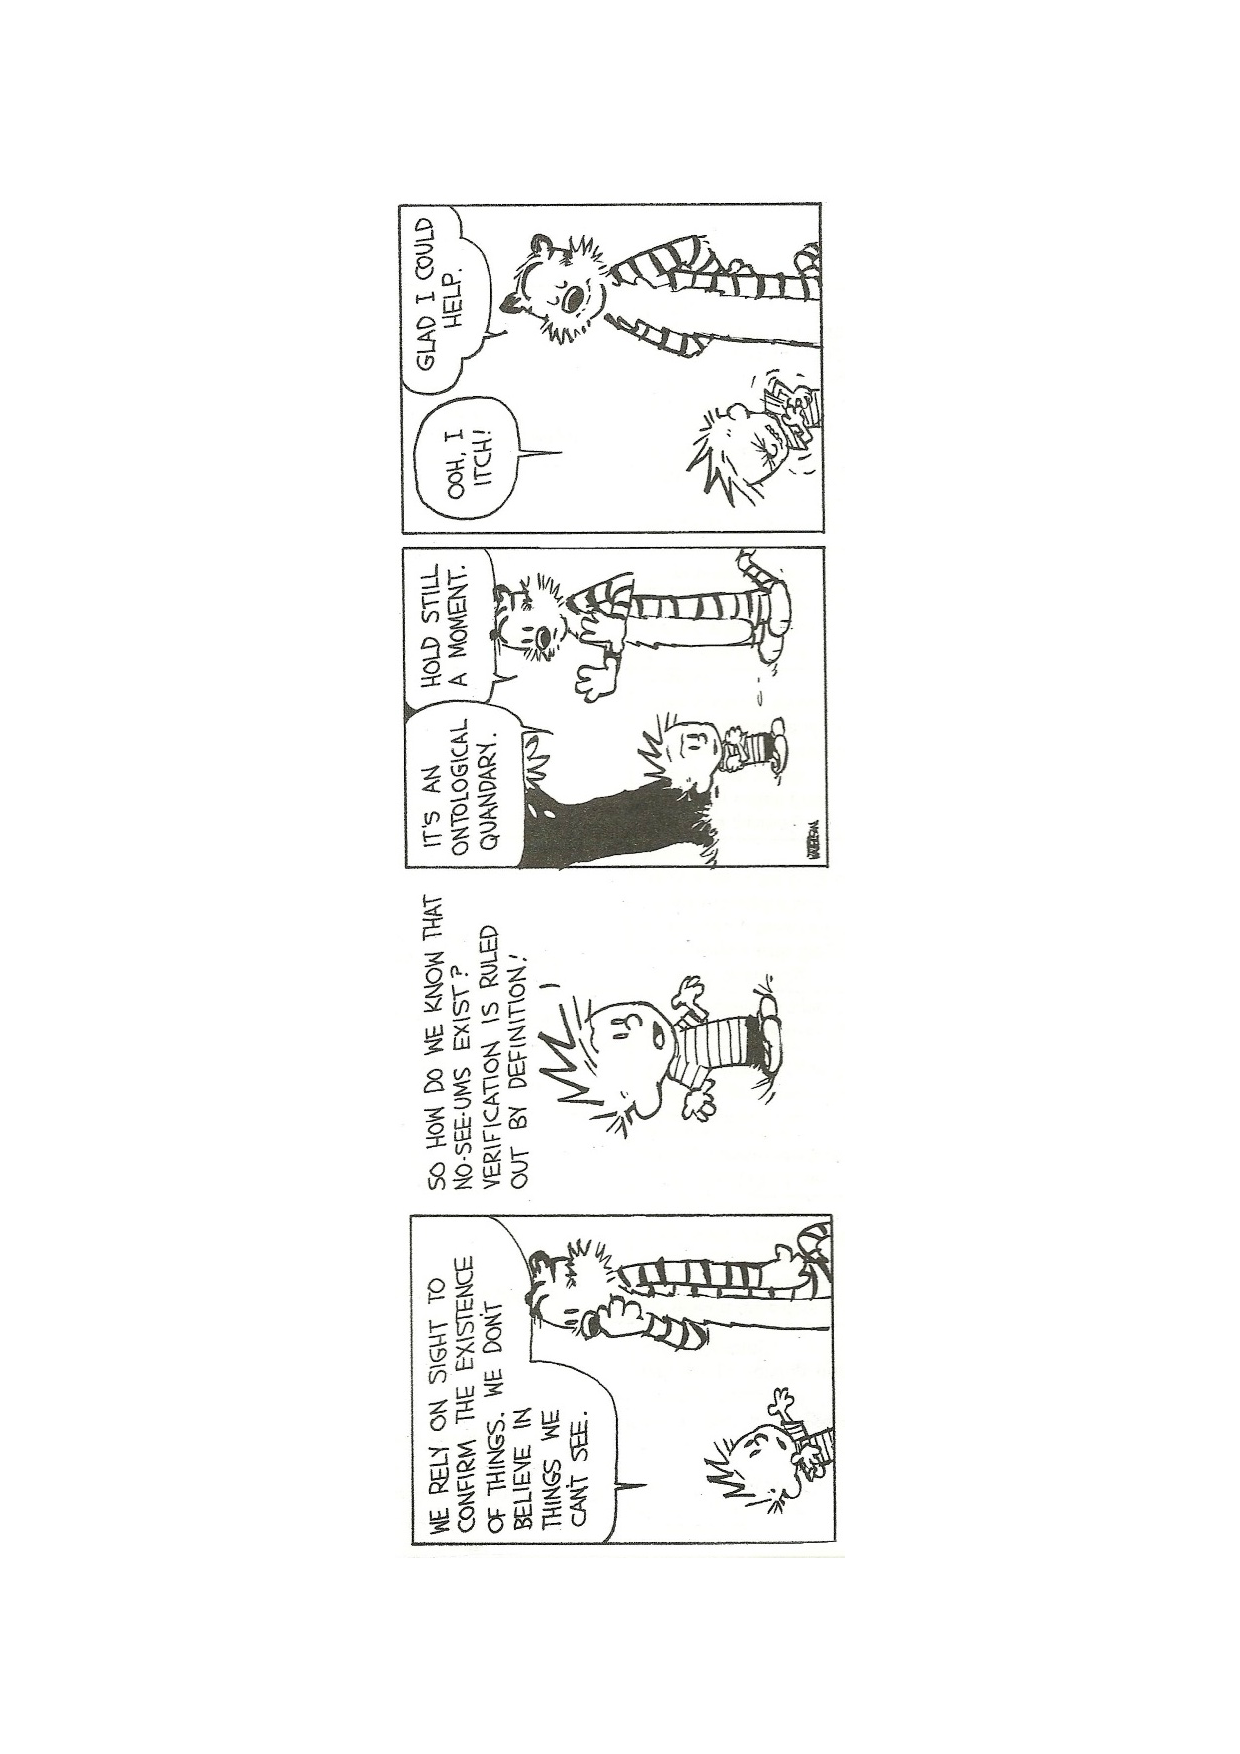
\includegraphics[width=0.7\textwidth,angle =-90]{calvin-and-hobbes}
%	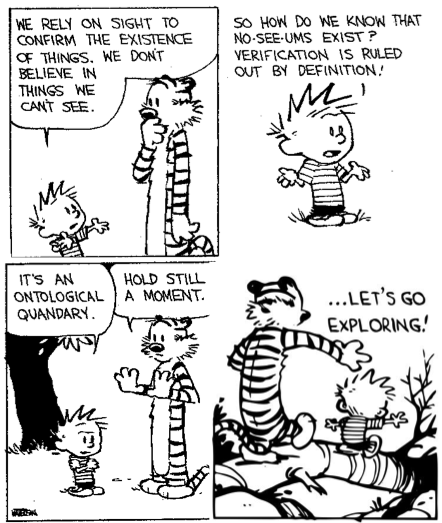
\includegraphics[width=0.7\textwidth]{./intro}
%	%	\caption{}
%	%	\label{fig:calvin-and-hobbes}
%\end{figure*}
%\vfill

\begin{figure*}[tbph]
		\centering
       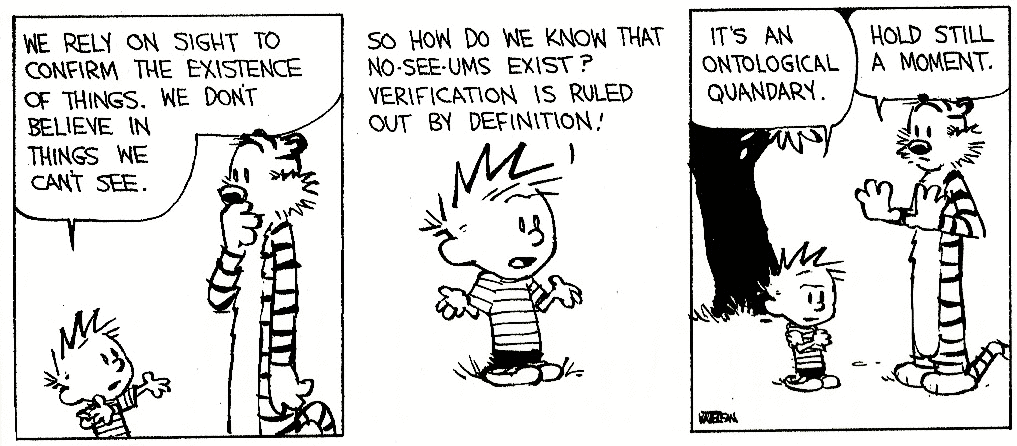
\includegraphics[width=0.6\linewidth]{./holdstill}
   	    
\includegraphics[width=0.6\linewidth]{./CALVINandHOBBES_LETS_GO_EXPLORING_original_grande}
		%	\caption{}
		%	\label{fig:calvin-and-hobbes}
		
\end{figure*}
\vfill

\cleardoublepage
% -------------------------------------------------- %
%    the main content                                %
% -------------------------------------------------- %

\mainmatter
\chapter{Theoretical basis}
% top quark 
% http://www.slac.stanford.edu/pubs/slacreports/reports03/ssi95-001.pdf
%https://d22izw7byeupn1.cloudfront.net/files/RevModPhys.69.137.pdf
%Disentangling Heavy Flavor at Colliders
% https://arxiv.org/abs/1702.02947

%Why dim 6 operators? 
%https://indico.cern.ch/event/610458/#4-top-16-017-eft-re-interpreta
% particle physics
%http://www.hep.phy.cam.ac.uk/~thomson/lectures/partIIIparticles/Handout13_2009.pdf
%EFT Theory
%https://indico.cern.ch/event/537012/timetable/#day-2016-11-23
%https://indico.cern.ch/event/612805/

%eft interpretation 
% https://mail.google.com/mail/u/0/?tab=wm#inbox/15b57592ac482483
% https://twiki.cern.ch/twiki/bin/view/CMS/TopEFT
The Standard Model (\SM)~\cite{Peskin:257493} 
is a name given in the 1970s to a theory describing the fundamental particles and their interactions. This quantum field theory describes the particles and their interactions as fields and has successfully incorporated three of the four fundamental forces in the universe. In \Sec{sec:SMcontent}, the particle content of the \SM\ is summarised, while \Sec{sec:SMlagr} describes  the \SM\ Lagrangian and its symmetries. In \Sec{sec:FCNC}, the flavour content of the \SM\ is highlighted, and \Sec{sec:top} focusses on the top quark in the \SM. 

The successful theory of the \SM\ has some shortcomings which are discussed in \Sec{sec:BSM} and lead to searches for a more general theory. One of such  is using  an effective field theory (EFT) approach~\cite{Burgess:2007pt}  to search for new physics in a model independent way. In \Sec{sec:EFT} an EFT model focussing on flavour changing neutral currents (FCNC) involving a top quark is presented. Its current experimental constraints are given in \Sec{sec:ExpConstr}.



\section{Elementary particles and forces}
\label{sec:SMcontent}
The interactions in nature can be described by four forces, the strong force, the electromagnetic (EM) force, the weak force and the gravitational force. These interactions happen via particles with an integer spin known as bosons. The strong interaction is mediated by eight gluons \Pgluon, while the electromagnetic force is mediated by photons \Pphoton, and the weak force by \PZ and \PWpm bosons. In \tab{tab:forces}, the forces and their characteristics are shown. The gravitational force is the only force not included in the \SM\ and can be neglected for energies lower than the Planck scale (1.22 $\times 10^{19}$~\GeV).
\begin{table}[htbp]
	\centering
	\caption{The four forces of nature and their characteristics.}
	\begin{tabular}{lcc}
		\toprule
		& Range & Mediator \\ 
		\midrule
		Strong force & $10^{-15}$ \m & 8 gluons  \\ 
	
		Electromagnetic force & $\infty$ & photon  \\ 
		 
		Weak force & $10^{-18}$ \m & \PWpm, \PZ bosons \\ 
		
		Gravitational force & $\infty$ & unknown \\ 
		\bottomrule
	\end{tabular} 
	\label{tab:forces}
\end{table}

The fermions are the particles that make up the visible matter in the universe. They carry half integer spin and can be subdivided into leptons and quarks, where leptons do not interact strongly. Each fermion has a corresponding anti-fermion which has the same mass and is oppositely charged. The electron \Pe\ is the first elementary particle discovered~\cite{electrondiscovery} and belongs to the first generation of leptons together with the electron neutrino \Pnue. The second generation comprises the muon \Pmu\ and muon neutrino \Pnum, whereas the third generation consists of the tau \Ptau and  tau neutrino \Pnut. The neutrinos are neutral particles, while the other leptons have charge $\pm \qe$ with \qe representing the elementary charge of 1.602 $\times 10^{-19}$ C. The masses of charged leptons differ by four orders of magnitude between the first and third generations. In the \SM\ the neutrinos are assumed to be massless, nonetheless it is experimentally established that neutrinos do have a tiny non-zero mass~~\cite{Fukuda:1998mi,PhysRevLett.108.131801}. In \tab{tab:leptongen}, the leptons and their properties in the \SM\ are summarised. 
\begin{table}[htbp]
	\centering
	\caption{The properties of the leptons in the three generations of the \SM~\cite{PDG}, where \qe represents the elementary  charge.}
	\begin{tabular}{lccc}
		\toprule
		Generation & Particle  & Mass  & Charge \\ 
		\midrule
		\multirow{2}{*}{First} & \Pelectron & 0.511 \MeV & -\qe  \\ 
		& \Pnue & $\approx$ 0 & 0\\
		
	\multirow{2}{*}{Second} & \Pmuon & 106 \MeV &-\qe  \\ 
	& \Pnum & $\approx$ 0 & 0\\
	
	\multirow{2}{*}{Third} & \Ptauon & 1 777 \MeV & -\qe  \\ 
	& \Pnut & $\approx$ 0 & 0 \\
	
		
		\bottomrule
	\end{tabular} 
	\label{tab:leptongen}
\end{table}

The quarks can also be divided into three generations. Unlike the leptons, they carry colour charge and can interact via the strong interaction. The top quark, discovered in 1995 at the Tevatron~\cite{observationtopD0,observationtopCDF}, is the heaviest \SM\ particle with a mass\footnote{In this thesis all masses and energies are expressed in natural units, where the speed of light and $\hbar$ are taken to be equal to one.} measured to be $173.34\pm0.27$(stat)$\pm0.71$(syst)~\GeV~\cite{ATLAS:2014wva}. The quarks and their properties are summarised in \tab{tab:quarkgen}. In nature, only colour neutral objects can exist. This has as consequence that quarks are bound through gluons into mesons (quark+anti-quark) and baryons (three quarks). These mesons and baryons are mostly short-lived and unstable particles that rapidly decay through \PWpm\ and \PZ\ bosons. The only known stable baryon is the proton, made up of two up quarks and one down quark.  
\begin{table}[htbp]
	\centering
	\caption{The properties of the quarks in the three generations of the \SM~\cite{PDG}, where \qe represents the elementary  charge.}
	\begin{tabular}{lccc}
		\toprule
		Generation & Particle  & Mass  & Charge \\ 
		\midrule
		\multirow{2}{*}{First} & up \Pup &$2.2_{-0.4}^{+0.6}$ \MeV& $\textfrac{2}{3}$ \qe  \\ 
		& down \Pdown & $4.7^{+0.5}_{-0.4}$ \MeV & $\textfrac{-1}{3}$ \qe\\
		
		\multirow{2}{*}{Second} & charm \Pcharm & 1.28 $\pm$ 0.03~\GeV &$\textfrac{2}{3}$ \qe  \\ 
		& strange \Pstrange & $96^{+8}_{-4}$ \MeV & $\textfrac{-1}{3}$ \qe\\
		
		\multirow{2}{*}{Third} & top \Ptop & 173.1 $\pm$ 0.6~\GeV &$\textfrac{2}{3}$ \qe  \\ 
		&bottom \Pbottom & $4.18^{+0.04}_{-0.03}$~\GeV & $\textfrac{-1}{3}$ \qe \\
		
		
		\bottomrule
	\end{tabular} 
	\label{tab:quarkgen}
\end{table}

The scalar boson, commonly known as the Higgs boson, is the last piece of the \SM\ discovered in 2012~\cite{Chatrchyan:2012xdj,Aad:2012tfa}. It is responsible for the masses of the \PWpm and \PZ boson, and that of the fermions.

\newpage
\section{Standard Model Lagrangian, connecting fields with particles}
\label{sec:SMlagr}
The \SM\ is a quantum field theory and thus describes the dynamics and kinematics of particles and forces by a Lagrangian \Lagr. The theory is based on the \SSU\ gauge symmetry, where \SU\ describes the electroweak interaction and \Sthree\ the strong interaction. The indices refer to colour C, the left chiral nature of the \Stwo\ coupling L, and the weak hypercharge Y. Its Lagrangian is constructed such that symmetries representing physics conservation laws such as conservation of energy, momentum and angular momentum are contained. The symmetries under local gauge transformations are sustained by demanding gauge invariance\footnote{Different field configurations of unobservable fields can result in identical quantities. Transformations between such configurations are called gauge transformation and the absence of change in the measurable quantities is a characteristic called gauge invariance.}.  



The \Uone\ group has one generator Y with an associated gauge field \Bfield. The three gauge fields \Wfieldone, \Wfieldtwo, and \Wfieldthree, are associated to \Stwo\ with three generators that can can  be written as half of the Pauli matrices: 
\begin{equation}
T_1 =  \frac{1}{2}
\begin{pmatrix}
0  &  1      \\
1  & 0      
\end{pmatrix}, \;
T_2= \frac{1}{2}
\begin{pmatrix}
0  &  -i     \\
i  &  0      
\end{pmatrix},\;\mathrm{ and } \;
 T_3= \frac{1}{2}
 \begin{pmatrix}
 1  &  0     \\
 0  &  -1 
 \end{pmatrix}.
 \label{eq:Stwee}
\end{equation}
The generators $T^a$ satisfy the Lie algebra: 
\begin{equation}
 \left[T_a,T_b\right] = i \epsilon_{abc} T^c \; \mathrm{ and } \left[T_a, Y\right] = 0, 
\end{equation}
where $\epsilon_{abc}$ is an antisymmetric tensor. The gauge fields of \Stwo\ only couple to left-handed fermions as required by the observed parity violating nature of the weak force. The \Sthree\ group represents quantum chromodynamics (QCD). It  has eight generators corresponding to eight gluon fields \Gfields. Unlike \SU, \Sthree\ is not chiral. 

Under \Sthree\, quarks are colour triplets while leptons are colour singlets. This implies that the quarks carry a colour index ranging between one and three, whereas leptons do not take part in strong interactions. Based on the chirality, the quarks and leptons are organized in doublets or singlets. Each generation $i$ of fermions consists of left-handed doublets and right-handed singlets: 
\begin{equation}
\mathrm{l}_{\mathrm{L,i}} =  
\begin{pmatrix}
\Pe_{\mathrm{L,i}}       \\
\Pneutrino_{\mathrm{L,i}}     
\end{pmatrix}, \; \Pe_{\mathrm{R,i}}, \; \mathrm{q}_{\mathrm{L,i}} = 
\begin{pmatrix}
\Pup_{\mathrm{L,i}}       \\
\Pdown_{\mathrm{L,i}}     
\end{pmatrix}, \; \Pup_{\mathrm{R,i}}, \; \mathrm{and} \; \Pdown_{\mathrm{R,i}}
\end{equation}

The \SM\ Lagrangian can be decomposed as a sum of four terms
\begin{equation}
\lagr_{\mathrm{SM}} = \lagr_{\mathrm{gauge}} + \lagr_{\mathrm{f}} + \lagr_{\mathrm{Yuk}} + \lagr_{\phi}, 
\end{equation}
that are related to the gauge, fermion, Yukawa and scalar sectors. The gauge Lagrangian regroups the gauge fields of all three symmetry groups, and the fermionic part consists of kinetic energy terms for quarks and leptons. The interaction between fermions and the scalar doublet $\phi$ gives rise to fermion masses and is described by the Yukawa Lagrangian. The scalar part of the Lagrangian is composed of a kinematic and potential component related to the scalar boson. 
%\begin{equation}
% \lagr_{\mathrm{gauge}} = -\frac{-1}{4} \Gtensord \Gtensoru -\frac{-1}{4} \Wtensord \Wtensoru - -\frac{-1}{4} \Btensord \Btensoru, 
%\end{equation}
%where the tensors are
%\begin{align}
%\Gtensord &= \partial_{\mu}\mathrm{G}_{\nu}^{\mathrm{i}} - \partial_{\nu}\mathrm{G}_{\mu}^{\mathrm{i}} - g_{\mathrm{s}} f_{ijk} \mathrm{G}_{\mu}^j \mathrm{G}_{\nu}^k, \; \mathrm{ with }\; i,j,k = 1,...,8 \\
%\Wtensord &= \partial_{\mu}\mathrm{W}_{\nu}^{\mathrm{i}} - \partial_{\nu}\mathrm{W}_{\mu}^{\mathrm{i}} - g_{\mathrm{s}} \epsilon_{ijk} \mathrm{W}_{\mu}^j \mathrm{G}_{\nu}^k, \; \mathrm{ with }\; i,j,k = 1,...,8 \\
%\end{align}

For the electroweak theory, two coupling constants are introduced, namely $g'$ for \Uone\ and $g$ for \Stwo. The physically observable gauge bosons of this theory are the photon field \photonfield, the \PZ\ boson field \Zfield, and the \PW\ boson fields \Wfield. These are a superposition of the four gauge fields of \SU: 
\begin{equation}
\begin{aligned}
\photonfield &= \sW \Wfieldthree + \cW \Bfield, \\
 \Zfield &= \cW \Wfieldthree - \sW \Bfield, \; \mathrm{ and } \\
  \Wfield &= \sqrt{\frac{1}{2}}\left(\Wfieldone\mp i \Wfieldtwo\right), 
\end{aligned}
\end{equation}
where $\theta_{\mathrm{W}}$ represents the weak mixing angle defined as $\mathrm{tan}\; \theta_{\mathrm{W}} = \frac{g'}{g}$.

The coupling constant representing the strength of the QCD interactions is denoted as $g_{\mathrm{s}}$. In QCD there is asymptotic freedom whereby the strong coupling constant becomes weaker as the energy with which the interaction between strongly interacting particles is probed increases, and stronger as the distance between the particles increases. A consequence of this is known as colour confinement, the quarks and gluons can not exist on their own and are not observed individually. They are bound in colour neutral states called hadrons, this process is known as hadronisation. 






\subsection*{Electroweak symmetry breaking}
In $\lagr_{\mathrm{gauge}}$ and $\lagr_{\mathrm{f}}$ are no mass terms for fermions present because only singlets under \SSU\ can acquire a mass with an interaction of the type $m^2\phi^{\dagger}\phi$ without breaking the gauge invariance. In order to accommodate mass terms for fermions and gauge fields, electroweak symmetry breaking, leading to $\lagr_{\phi}$ is introduced. 

The scalar doublet is introduced in the \SM\ as 
\begin{equation}
\phi = \frac{1}{\sqrt{2}}
\begin{pmatrix}
\varphi_1 + i \varphi_2    \\
\varphi_3 + i \varphi_4    
\end{pmatrix}.
\end{equation}
Its field potential is of the form 
\begin{equation}
V(\phi) = \mu^2 \phi^{\dagger}\phi + \lambda(\phi^{\dagger}\phi)^2, 
\end{equation}
with $\mu^{2} <0$ and $\lambda$ a positive integer. This choice of parameters gives the potential a "Mexican hat" shape. It has an infinite set of minima (ground states) and by expanding the field around an arbitrary choice of ground state, the electroweak symmetry is broken (\cancel{EW}): 
\begin{equation}
\phi = 
\begin{pmatrix}
0    \\
\frac{v}{\sqrt{2}}    
\end{pmatrix}
+ \hat{\phi}, 
\end{equation}
where $v$ is the vacuum expectation value (vev), measured to be around 245~\GeV\ and corresponds to $\sqrt{\frac{-\mu}{\lambda}}$. The scalar doublet's four degrees of freedom are reduced to three degrees of freedom that couple to the gauge fields and fix the \PWp, \PWm and \PZ bosons. The remaining fourth degree of freedom has given rise to a physically observable particle, called the Brout-Englert-Higgs (BEH) boson.
This spontaneous symmetry breaking leaves the gauge invariance intact and gives masses to the \PWpm and \PZ bosons as:
\begin{equation}
m_{\PW} = \frac{1}{2}v|g| \quad \mathrm{and} \quad m_{\PZ} = \frac{1}{2}v \sqrt{g'^2 + g^2}.
\end{equation}
The Brout-Englert-Higgs field couples universally to fermions with a strength proportional to their masses, and to gauge bosons with a strength proportional to the square of their masses. 


\section{Flavours in the \SM}
\label{sec:FCNC}
%In the electroweak theory, the \PW boson is responsible for flavour changing charged currents, and the \PZ boson for 
%lading W -> smamak veranderen -> niet voor Z , integendeel verboden op tree level onderdrukt op higher order
Flavour changing charged currents are introduced in 1963 by Nicola Cabibbo~\cite{PhysRevLett.10.531}. Via interactions with a \PW boson the flavour of the quarks is changed. At the time of the postulation only up, down,  and strange quarks were known and the charged weak current was described as a coupling between the up quark and $\Pdown_{\mathrm{weak}}$, where $\Pdown_{\mathrm{weak}}$ is a linear combination of the down and strange quarks, $\Pdown_{\mathrm{weak}}= \mathrm{cos }\theta_{\mathrm{c}} \Pdown + \mathrm{sin }\theta_{\mathrm{c}} \Pstrange$. This linear combination is a direct consequence of the chosen rotation
\begin{equation}
\begin{pmatrix}
\Pdown_{\mathrm{weak}} \\
\Pstrange_{\mathrm{weak}} 
\end{pmatrix}
 = 
 \begin{pmatrix}
 \mathrm{cos }\theta_{\mathrm{c}} &  \mathrm{sin }\theta_{\mathrm{c}} \\
 - \mathrm{sin }\theta_{\mathrm{c}} &  \mathrm{cos }\theta_{\mathrm{c}}
 \end{pmatrix}
 \begin{pmatrix}
 \Pdown \\
 \Pstrange 
 \end{pmatrix} = \mathcal{R} 
 \begin{pmatrix}
 \Pdown \\
 \Pstrange 
 \end{pmatrix}, 
\end{equation}
where the rotation angle $\theta_{\mathrm{c}}$ is known as the Cabibbo angle. This provides a definition for the charged weak current between \Pup\ and \Pdown\ quarks, 
\begin{equation}
J_{\mu} = \APup \gamma_{\mu}\left(1+\gamma_5\right)\Pdown_{\mathrm{weak}}. 
\end{equation} 
A consequence of Cabibbo's approach is that the $\Pstrange_{\mathrm{weak}}$ is left uncoupled, leading to Glashow, Iliopoulos and Maiani (GIM)~\cite{PhysRevD.2.1285,BJORKEN1964255,Maiani:2013fpa} to require the existence of a fourth quark with charge $\textfrac{2}{3}\mathrm{q}_{\mathrm{e}}$. This quark, known as the charm quark, couples to $\Pstrange_{\mathrm{weak}}$ and a new definition of the charged weak current is modified to 
\begin{equation}
J_{\mu} = \begin{pmatrix}
\APup & \APcharm
\end{pmatrix}  \gamma_{\mu}\left(1+\gamma_5\right)\mathcal{R}  \begin{pmatrix}
d \\ s
\end{pmatrix}
= \bar{U} \gamma_{\mu}\left(1+\gamma_5\right)\mathcal{R}D. 
\end{equation} 

The neutral weak current is defined as 
\begin{equation}
J_{3} = \bar{U} \gamma_{\mu}\left(1+\gamma_5\right)\left[\mathcal{R}, \mathcal{R}^{\dagger}\right]D, 
\end{equation} 
and is diagonal in flavour space. This has as consequence that no flavour changing neutral currents occur at tree-level interactions~\cite{Peskin:257493}.


Kobayashi and Maskawa generalised the Cabibbo rotation matrix to accommodate a third generation of quarks. The result is a $3\times 3$ unitary matrix known as the CKM matrix, responsible for the mixing of weak interaction states of down-type quarks: 
\begin{equation}
\begin{pmatrix}
\Pdown_{\mathrm{weak}} \\
\Pstrange_{\mathrm{weak}} \\
\Pbottom_{\mathrm{weak}}
\end{pmatrix}
= 
\begin{pmatrix}
V_{\Pup\Pdown} & V_{\Pup\Pstrange} & V_{\Pup\Pbottom} \\
V_{\Pcharm\Pdown} & V_{\Pcharm\Pstrange} & V_{\Pcharm\Pbottom} \\
V_{\Ptop\Pdown} & V_{\Ptop\Pstrange} & V_{\Ptop\Pbottom}
\end{pmatrix}
\begin{pmatrix}
\Pdown \\
\Pstrange \\
\Pbottom
\end{pmatrix} = \mathcal{V}_{\mathrm{CKM}} \begin{pmatrix}
\Pdown \\
\Pstrange \\
\Pbottom
\end{pmatrix},
\end{equation}
where $\mathcal{V}_{\mathrm{CKM}}$ is unitary ($\mathcal{V}_{\mathrm{CKM}}^{\dagger}\mathcal{V}_{\mathrm{CKM}} = \mathbb{1}$). A general $3\times 3$ unitary matrix depends on three real angles and six phases. For the CKM matrix, the freedom to redefine the phases of the quark eigenstates can remove fives of the phases, leaving a single physical phase known as the Kobayashi-Maskawa phase. This phase is responsible for the charge parity violation in the \SM~\cite{CKM}. 
% see wolfenstein parametrisation http://pdg.lbl.gov/2017/reviews/rpp2016-rev-cp-violation.pdf 13,53
Each element $V_{\mathrm{ij}}$ of $ \mathcal{V}_{\mathrm{CKM}}$ represents the transition probability of a quark i going to a quark j, and is experimentally determined to be~\cite{PDG}
\begin{equation}
\mathcal{V}_{\mathrm{CKM}} =
\begin{pmatrix}
0.97425 \pm 0.00022  & 0.2253 \pm 0.0008      & (4.13 \pm 0.49) \times 10^{-3} \\
0.225 \pm 0.008      & 0.986 \pm 0.016        & (41.1 \pm 1.3) \times 10^{-3} \\
(8.4\pm 0.6) \times 10^{-3} & (40.0 \pm 2.7) \;10^{-3} & 1.021 \pm 0.032
\end{pmatrix}.
\label{eq:CKM}
\end{equation}

From  \eq{eq:CKM} follows that top quarks predominantly decay via charged weak currents to bottom quarks, with a probability consistent with unity. In the \SM, FCNC can only occur via higher loop interactions which are highly suppressed. The expected transition probabilities for a top quark decaying via a FCNC interaction in the \SM\ are given in \tab{tab:FCNCBR}, where it is clear that the FCNC top quark interactions of the \SM\ is still beyond the reach of the sensitivity of current experiments. 
\begin{table}[htbp]
	\centering
	\caption{The predicted branching ratios \BR\ for FCNC decays involving the top quark in the \SM~\cite{AguilarSaavedra:2004wm}.}
	\begin{tabular}{lc|lc}
		\toprule
	    Process	& \BR\ in the \SM  &  Process	& \BR\ in the \SM \\ 
		\midrule
		$ \Ptop \rightarrow \Pup \PZ $         & $8  \times 10^{-17}$  &	$ \Ptop \rightarrow \Pcharm \PZ $      & $1  \times 10^{-14}$   \\
		$ \Ptop \rightarrow \Pup \Pphoton $    & $4  \times 10^{-16}$  & $ \Ptop \rightarrow \Pcharm \Pphoton $ & $5  \times 10^{-14}$   \\
		$ \Ptop \rightarrow \Pup \Pgluon $     & $4  \times 10^{-14}$  & $ \Ptop \rightarrow \Pcharm \Pgluon $  & $5  \times 10^{-12}$  \\
		$ \Ptop \rightarrow \Pup \PHiggs $     & $2  \times 10^{-17}$  & $ \Ptop \rightarrow \Pcharm \PHiggs $  & $3  \times 10^{-15}$ \\
		\bottomrule
	\end{tabular} 
	\label{tab:FCNCBR}
\end{table}

\section{The top quark in the \SM}
\label{sec:top}
\label{sec:TopSM}
Discovered in 1995 by the CDF and D0 collaborations at the Tevatron with proton-antiproton data~\cite{Abachi:1995iq,Abe:1995hr,}, the top quark plays an important role in studying high energy physics. Its Yukawa interaction is given by
\begin{equation}
\lagr_{\mathrm{top-Yukawa}} = -\frac{\lambda_t v}{\sqrt{2}} \APtop_{\mathrm{L}} \Ptop_{\mathrm{R}} -\frac{\lambda_{\Ptop} }{\sqrt{2}} \PHiggs \APtop_{\mathrm{L}} \Ptop_{\mathrm{R}} + \mathrm{h.c.},
\end{equation}
yielding a Yukawa coupling of~\cite{PDG}
\begin{equation}
 \lambda_{\mathrm{t}} = \frac{\sqrt{2}m_{\Ptop}}{v} = 0.991 \pm 0.003.
\end{equation}
 This Yukawa coupling is very large compared to the other Yukawa couplings in the SM (\order($10^{-2}$)), leading to the belief that the top quark may have an important role in understanding the mechanism of electroweak symmetry breaking. On top of this, the very short lifetime of the top quark makes it an excellent candidate to study the properties of a bare quark. Its high mass, almost 40 times higher than the mass of the closest fermion in mass, leads to a large coupling with the Higgs boson and makes the top quark an interesting candidate to investigate how particles acquire mass. 


The CKM matrix element $V_{\Ptop\Pbottom}$, given in \eq{eq:CKM}, is experimentally found to be much larger than $V_{\Ptop\Pstrange}$, $V_{\Ptop\Pdown}$, and close to unity. The top quark decays through electroweak interactions since the  \PW\ boson mass is smaller than the top quark mass and the \PW\ boson can be on shell. A consequence of this is that the top quark has a very short lifetime of only $1/\Gamma_{\Ptop}\approx 5 \: 10^{-25}$ \s~\cite{PDG} leading to the fact that the formation of bound states involving top quarks are not allowed. This lifetime is even shorter than the typical hadronisation timescale of $1/\Lambda_{\mathrm{QCD}}\approx 10^{-23}$ \s, prohibiting gluons to radiate from the top quark and keeping its spin coherent. Since the electroweak interactions have a vector-axial vector (V-A) coupling structure\footnote{In the \SM\ a vector - axial vector coupling structure $\left(\gamma^{\mu} - \gamma^{\mu}\gamma^5\right)$ is predicted  that only permits left-handed fermions  or right-handed anti fermions to interact with a spin-1 particle. }
%\footnote{For an interaction where a spin-1 particle is exchanged, the most general form is a linear combination of a vector and an axial vector. From experiments, the weak interaction is determined to have this V-A structure: $J^{\mu} \prop \APup_{\Pneutrino}\left(\gamma^{\mu} - \gamma^{\mu}\gamma^5\right)\Pup_{\Pe}$.}
, the top quark spin orientation can be derived from the angular distributions of its decay products. This makes it possible to study the polarisation of top quarks from the angular distributions in various processes. 


The massiveness of the top quark leads to the fact that a large amount of energy is needed to create one. This is only the case for high energy collisions such as those happening in the Earth's upper atmosphere when cosmic rays collide with particles in air, or by particle accelerators. The production of top quarks happens in two ways: single via the electroweak interaction or in pairs via the strong interaction. At hadron colliders, the dominant production mechanism is top quark production via gluon (gg$\rightarrow$\ttbar) or quark fusion (\qqbar $\rightarrow$ \ttbar). In \fig{fig:toppairproduction}, the different top quark pair production mechanisms are shown. The production channel of gluon fusion is the main contributor to the top quark pair cross section at the LHC compared to quark fusion at the Tevatron. % because of the increasing gluon PDF towards smaller momentum fraction
The gg$\rightarrow$\ttbar\ process contributes 80-90\% to the total top quark pair cross section in the LHC centre-of-mass energy regime of 7-14~\TeV~\cite{PDG}. In \tab{tab:toppaircros} the predicted top quark pair production cross sections are given for the LHC and the Tevatron, while in \fig{fig:ttcross}, a summary plot of the LHC and Tevatron top quark pair cross section measurements as a function of the centre-of-mass energy can be found.
%\begin{figure}[htbp]
%	\centering
%	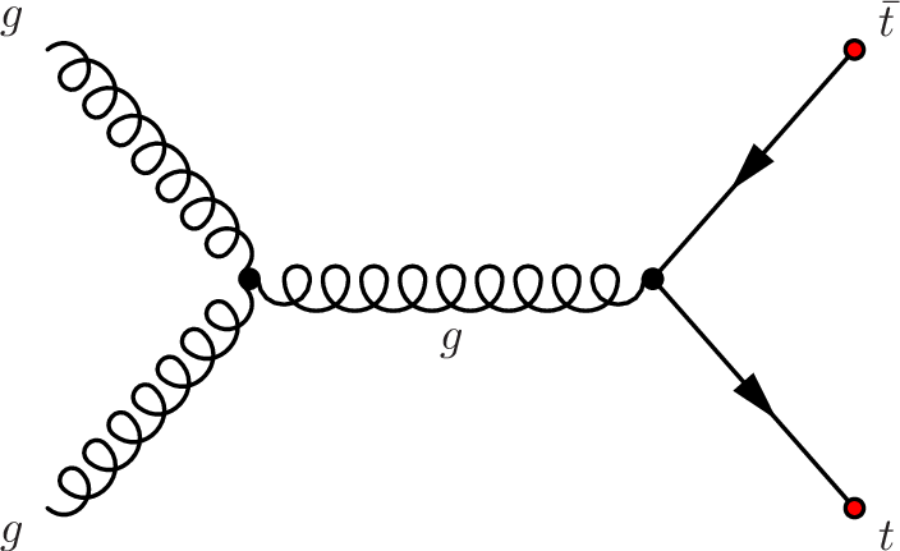
\includegraphics[width=0.32\linewidth]{1_Introduction/Figures/Ttbar_production_via_gg_fusion}
%	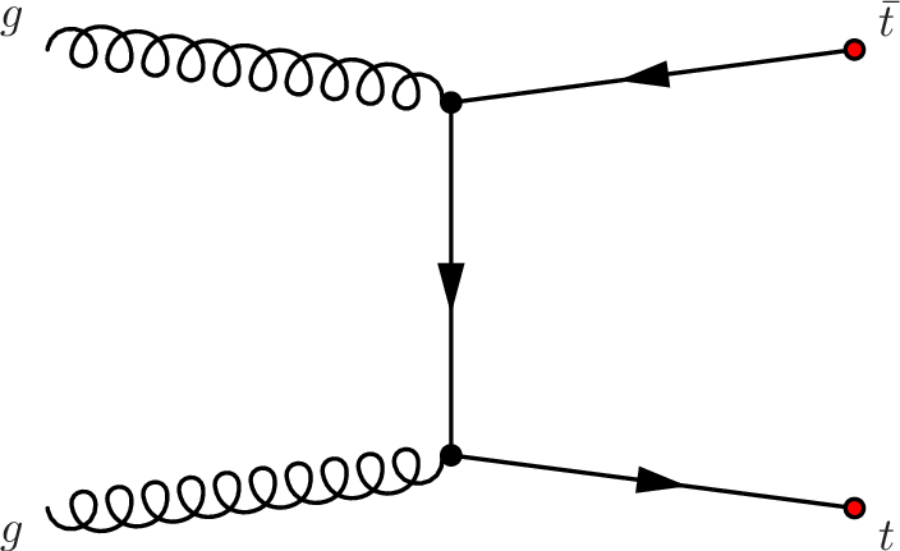
\includegraphics[width=0.32\linewidth]{1_Introduction/Figures/Ttbar_production_(t_channel)}
%	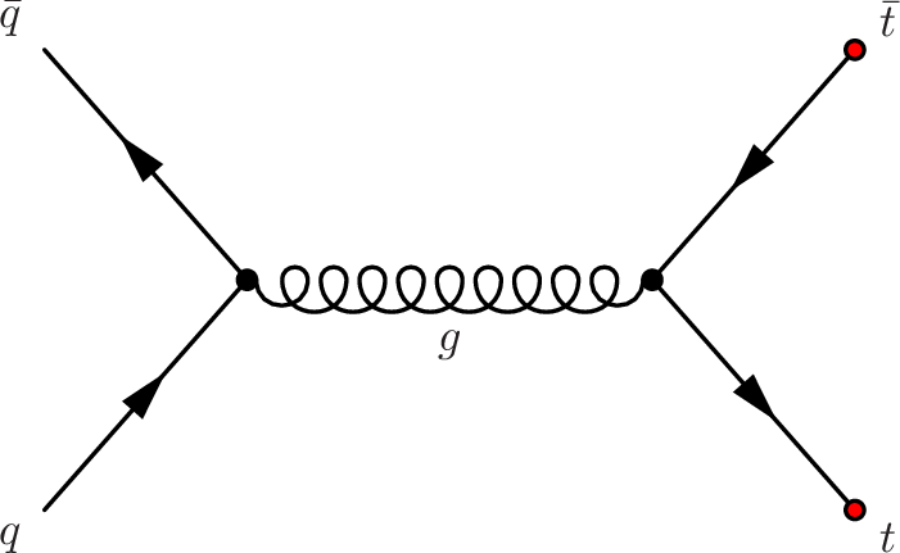
\includegraphics[width=0.32\linewidth]{1_Introduction/Figures/Ttbar_production_via_qqbar_annihilation}
%	\caption{Leading order diagrams of the top quark pair production. Gluon fusion (left and middle)are the dominant processes at the LHC, while quark fusion (right) is the dominant one at Tevatron. }
%	\label{fig:toppairproduction}
%\end{figure}
\begin{figure}[htbp]
	\centering
	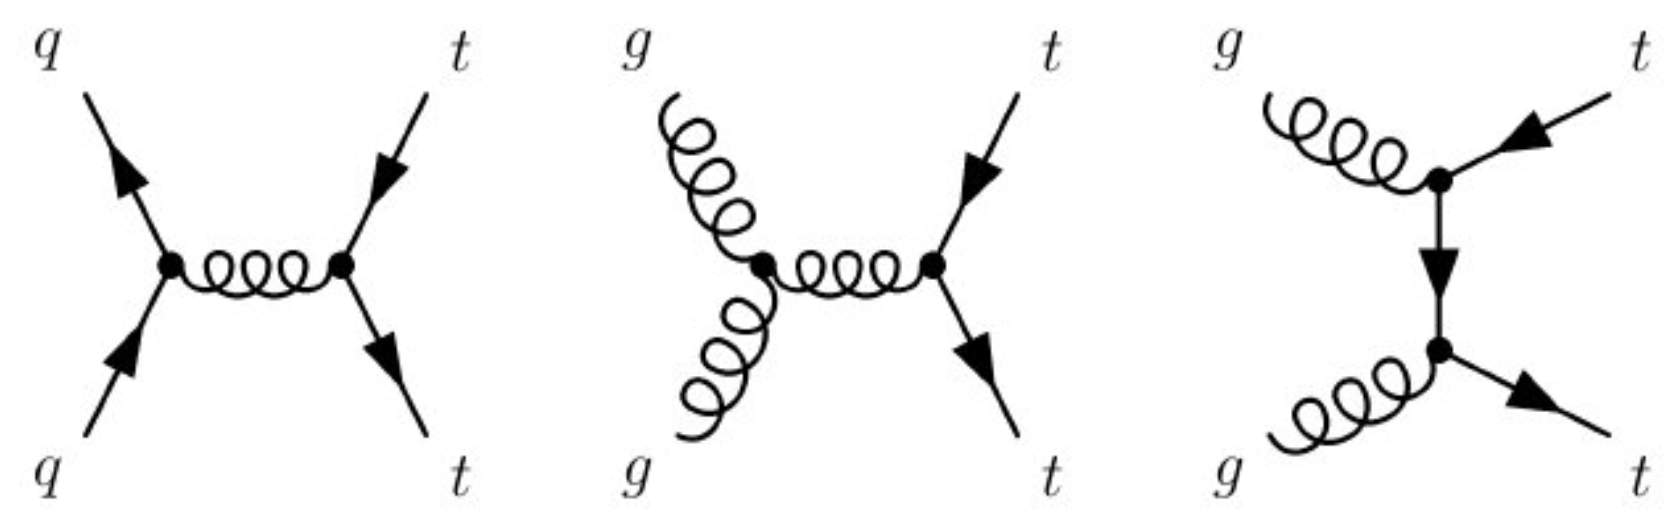
\includegraphics[width=0.7\linewidth]{1_Introduction/Figures/toppair}
	\caption{Leading order diagrams of the top quark pair production. Gluon fusion (right and middle) are the dominant processes at the LHC, while quark fusion (left) is the dominant one at the Tevatron. }
	\label{fig:toppairproduction}
\end{figure}
\begin{table}[htbp]
	\centering
	\caption{Predictions on the top quark pair production cross sections at next-to-next-to-leading order with next-to-next-to-leading log soft gluon resummation per centre-of-mass energy~\cite{PDG}. The first uncertainty is from scale dependence, while the second uncertainty originates from parton density functions.}
	\begin{tabular}{llll}
		\toprule
	 Experiment & Top quark mass &Centre-of-mass energy& Cross section (\pb) \\ 
		\midrule
		Tevatron & $m_{\Ptop} = 173.3 \:~\GeV$ & $\sqrt{s} = 1.96$~\TeV & $\sigma_{\ttbar} = 7.16^{+0.11+0.17}_{-0.20-0.12}$  \\ 
		LHC & $m_{\Ptop} = 173.2 \:~\GeV$ & $\sqrt{s} = 7$~\TeV & $\sigma_{\ttbar} =173.6^{+4.5+8.9}_{-5.9-8.9}$  \\
		LHC & $m_{\Ptop} = 173.2 \:~\GeV$ & $\sqrt{s} = 8$~\TeV & $\sigma_{\ttbar} =247.7^{+6.3+11.5}_{-8.5-11.5}$  \\
		LHC & $m_{\Ptop} = 173.2 \:~\GeV$ & $\sqrt{s} = 13$~\TeV & $\sigma_{\ttbar} =816.0^{+19.4+34.4}_{-28.6-34.4}$  \\
	\bottomrule
	%http://pdg.lbl.gov/2017/reviews/rpp2016-rev-top-quark.pdf
	\end{tabular} 
	\label{tab:toppaircros}
\end{table}

\begin{figure}[htbp]
	\centering
	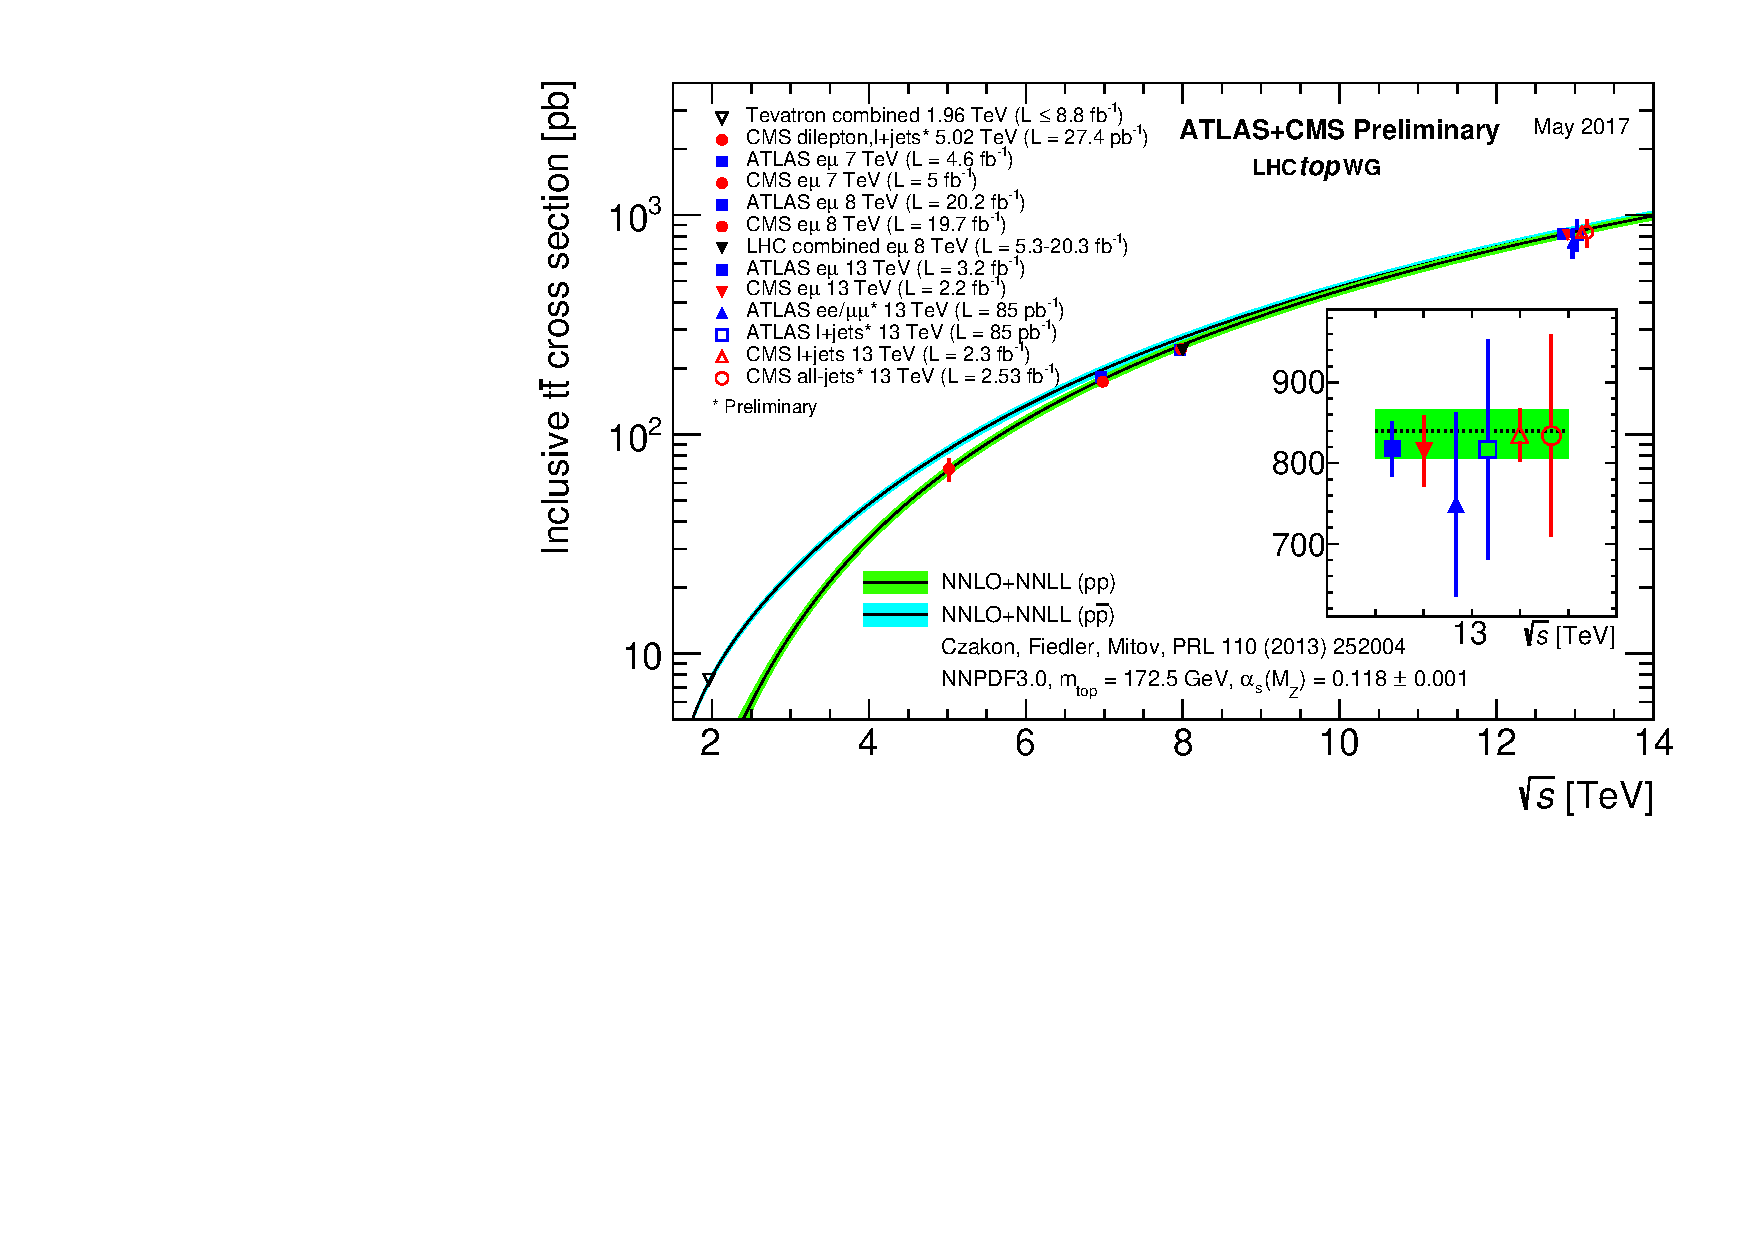
\includegraphics[width=1.\linewidth]{1_Introduction/Figures/tt_xsec_vsroots.pdf}
	\caption{Summary of the LHC and the Tevatron measurements of the top quark pair production cross section as function of the centre-of-mass energy compared with the next-to-next-to-leading order QCD calculation. The theory bands are the uncertainties due to renormalization and factorisation scales, parton density functions and the strong coupling. The mass of the top quark is assumed to be 172.5 \GeV. Measurements for the same centre-of-mass energy are slightly off-set for clarity.  Figure taken from \cite{summarytwiki}.}
		\label{fig:ttcross}
\end{figure}

The singly produced top quarks are produced via the electroweak interaction. These production mechanisms are subdivided at leading order into three main channels based on the virtuality ($Q^2 = - p_{\mu}p^{\mu}$) of the exchanged \PW\ boson. In \fig{fig:singletop}, the corresponding Feynman diagrams are shown. The single top quark production cross sections, given in \tab{tab:singletopcros}, are smaller than the top quark pair production cross sections since the electroweak coupling strength is smaller than the strong coupling strength. In addition, for the single top quark production, there is the need of sea quarks (\Pbottom, \APquark) in the initial states for which the parton density functions increase less steeply at low momentum fractions compared to the gluon parton density functions. 
\begin{comment}
	Electroweak single top-quark production mechanisms, na- mely from qq′ → tb [4], qb → q′t [5], mediated by virtual s-channel and t-channel W-bosons, and Wt-associated pro- duction, through bg → W−t, lead to somewhat smaller cross sections. For example, t-channel production, while suppressed by the weak coupling with respect to the strong pair produc- tion, is kinematically enhanced, resulting in a sizable cross section both at Tevatron and LHC energies. At the Tevatron, the t- and s-channel cross sections of top and antitop are identical, while at the LHC they are not, due to the charge- asymmetric initial state. 
\end{comment}
\begin{figure}[htbp]
	\centering
	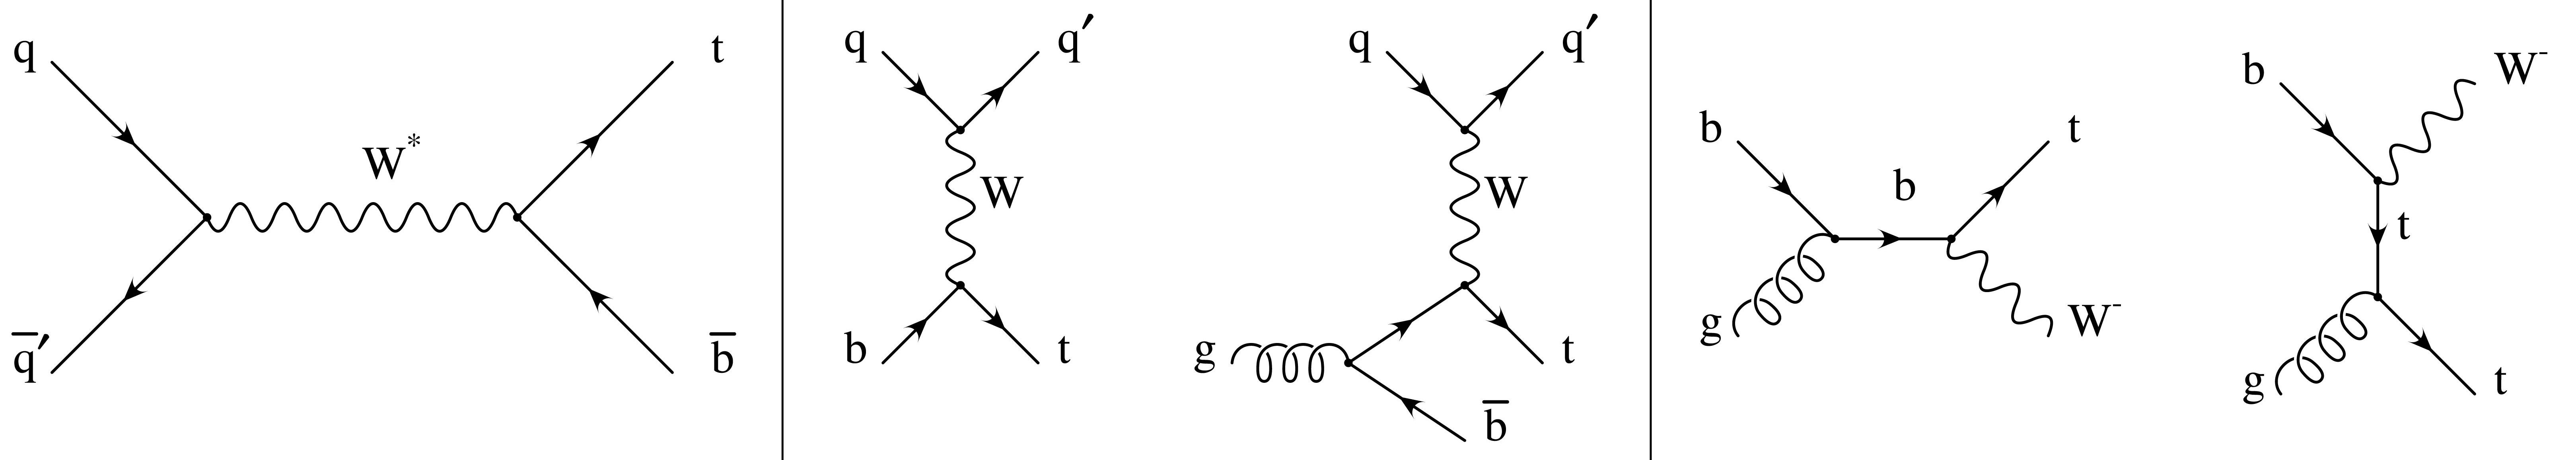
\includegraphics[width=1.\linewidth]{1_Introduction/Figures/single_Top_channels_0}
	\caption{Leading order Feynman diagrams of the electroweak production of single top quarks in the $s$-channel (left), $t$-channel (middle), and for the tW associated production. Figure taken from \cite{singletop}.}
	\label{fig:singletop}
\end{figure}

The production via the $t$-channel has a virtuality of the \PW\ boson $Q^2>0$, making it space-like. It is produced via the scattering of the \PW\ boson of a bottom quark coming from a proton or from gluon splitting (\Pgluon$\rightarrow$\bbbar). It has the highest single top quark cross section in proton collisions and the top quark production is roughly twice as large than the antitop quark. This is a consequence of the up-down valence quark composition of the proton. This feature makes the $t$-channel sensitive to the parton density functions of the proton. %The ratio depends however on the center-of-mass energy since at higher energies lower momentum fractions are probed at which contributions from the valence quarks become less dominant.
The $s$-channel is the production mechanism with the smallest cross section. Here the \PW\ boson is time-like ($Q^2 <0$) which requires the \PW\ boson to have a large virtuality to produce the heavier top quark. It is produced from two quarks belonging to the same isodoublet (e.g. \Pup\APdown) and subsequently decays to \Ptop\APbottom. This process gets enhanced by many beyond the Standard Model scenarios via the addition of new heavy particles such as \PW'. The tW-channel has a top quark produced in association with a \PW\ boson produced on shell $Q^2 = -m^2_{\PW}$. This mode is negligible at the Tevatron, but of relevant size at the LHC. The tW-channel is sensitive to new physics affecting the Wtb vertex.  The single top quark production cross section measurements by the CMS collaboration can be found in \fig{fig:stcross}.
 
 \begin{table}[htbp]
 	\centering
 	\caption{Predictions on the single top quark production cross sections at next-to-leading order per centre-of-mass energy~\cite{PDG}. The  uncertainties from scale dependence and from parton density functions are combined in quadrature or given separately (scale + PDF). For the $t$-channel the relative proportions to \Ptop\ and \APtop\ are 65\% and 35\%. For the $s$-channel this is respectively 69\% and 31\%. The tW-channel has an equal proportion of top and antitop quarks. For Tevatron, the top quark mass is assumed to be 173.3~\GeV, while the LHC predictions use $m_{\Ptop} = 172.5$~\GeV~\cite{PDG,stwiki}.} 
 	\begin{tabular}{lllll}
 		\toprule
 		Collider & Centre-of-mass energy& \multicolumn{3}{c}{Cross section $\sigma_{\Ptop+\APtop}$ (\pb)} \\ 
 		                     &                     &  $t$-channel & $s$-channel & tW-channel \\
 		\midrule
 		{Tevatron} & {$\sqrt{s} = 1.96$~\TeV }& $ 2.06^{+0.13}_{-0.13}$ &$  1.03^{+0.05}_{-0.05}$  & - \\ 
 		                        
 		{LHC} &{ $\sqrt{s} = 7$~\TeV }& $ 63.89^{+2.91}_{-2.52}$ &$  4.29^{+0.19}_{-0.17}$  & $ 15.74^{+0.40+1.10}_{-0.40-1.14}$ \\ 
 		{LHC} & { $\sqrt{s} = 8$~\TeV} & $ 84.69^{+3.76}_{-3.23}$ &$  5.24^{+0.22}_{-0.20}$  &  $ 22.37^{+0.60+1.40}_{-0.60-1.40}$  \\
 		{LHC} &  {$\sqrt{s} = 13$~\TeV }& $ 216.99^{+9.04}_{-7.71}$ &$  10.32^{+0.40}_{-0.36}$  &  $ 71.7^{+1.80+3.40}_{-1.80-3.40}$  \\ 
 		\bottomrule
 		%http://pdg.lbl.gov/2017/reviews/rpp2016-rev-top-quark.pdf
 		%https://twiki.cern.ch/twiki/bin/view/LHCPhysics/SingleTopRefXsec#Predictions_at_7_8_13_and_14_TeV
 	\end{tabular} 
 	\label{tab:singletopcros}
 \end{table}

\begin{figure}[htbp]
	\centering
	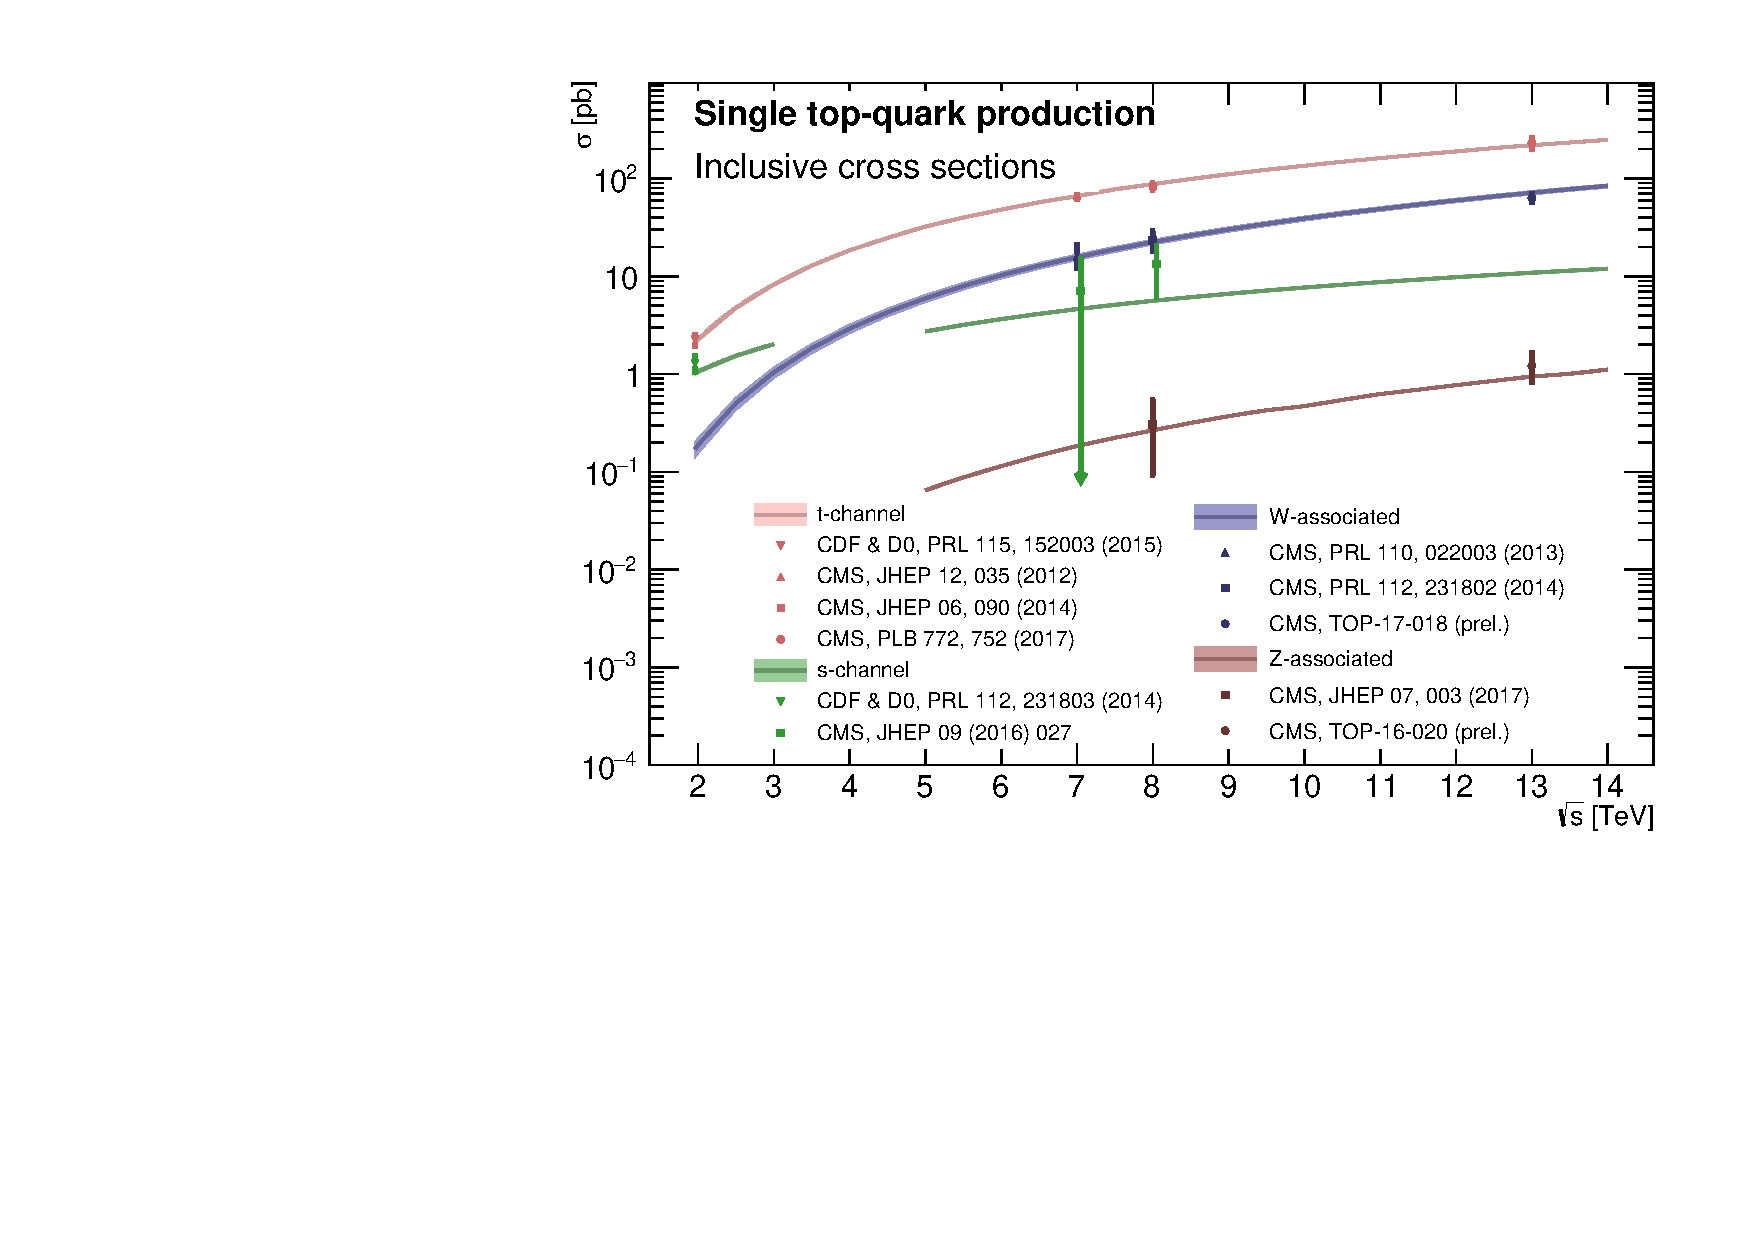
\includegraphics[width=1.\linewidth]{1_Introduction/Figures/singletop_sqrts.pdf}
	\caption{Summary of the measurements of the single top top quark production cross section as function of the centre-of-mass energy. Figure taken from \cite{summarywiki}.}
	\label{fig:stcross}
\end{figure}
\newpage
\section{Effective field theories}
%https://cp3.irmp.ucl.ac.be/upload/theses/phd/degrande.pdf
%http://www.physi.uni-heidelberg.de/Forschung/he/LHCb/documents/WorkshopNeckarzMarz08/TF_OPE.pdf
Problems can be simplified if one looks at the relevant scale of the process that one want to investigate, for example the chemical properties of an hydrogen atom can be described without any knowledge of quark interactions inside the proton. In this case, the proton can be considered the elementary object (indivisible) due to the fact that the binding energy of the constituents is much bigger than the energy of the electron in orbit around the proton. Effective field theories are based on this kind of separation of different energy scales in a system~\cite{thesisDeg}. Effective field theories can be used for theories where the perturbative expansion cannot be trusted, e.g. QCD at low energy, or as bottom up approach to look for new physics in a model independent way. The latter is the way effective field theory will be used throughout this thesis. 


The main idea behind effective field theory is easily explained via the example of the Fermi theory. Fermi explained in 1933~\cite{Fermi2008} the $\beta$-decay as a product of currents: 
\begin{equation}
\Lagr^{\mathrm{Fermi}}_{\mathrm{EFT}} = - \frac{G_{\mathrm{F}}}{\sqrt{2}} J^{\mu}J_{\mu}^{\dagger},
\label{eq:EFTfermi}
\end{equation}
where $G_{\mathrm{F}}$ is the Fermi coupling constant, measured to be $G_{\mathrm{F}} \approx 1.17 \times 10^{-5}~\GeV^{-2}$. The current $J_{\mu}$ can written as the sum of an hadronic $J_{\mu}^h$ and leptonic $J_{\mu}^l$ current, where for simplicity only the leptonic current discussed. 
\begin{equation}
	J_{\mu}^l = \sum \limits_{\mathrm{l}} \APnu_{\mathrm{l}} \gamma_{\mu} \left(1-\gamma_5\right) \mathrm{l}.
\end{equation}
Historically, charged currents were flavour universal and the later discovered parity violation of the weak interaction led to the V-A structure. After this, the \Stwo\ symmetry was postulated and the existence of neutral currents was predicted. The effective Lagrangian used then (given in \eq{eq:EFTfermi}), could nowadays be build starting from \Stwo\ symmetries only. 

The muon decay can be computed from two different starting points. The effective Fermi Lagrangian provides the decay width of the muon into an electron and two neutrinos 
\begin{equation}
	\Gamma(\Pmu \rightarrow \Pe\APnue\Pnum) \approx \frac{1}{96\pi^3} \frac{m_{\Pmu}^2}{\Lambda_{\mathrm{F}}^4},
	\label{eq:mudecay}
\end{equation}
where $\Lambda_{\mathrm{F}}$ is the energy scale defined as
\begin{equation}
	\frac{G_{\mathrm{F}}}{\sqrt{2}} = \frac{1}{\Lambda_{\mathrm{F}}^2}. 
\end{equation}
From muon decay measurements, the value of $\Lambda_{\mathrm{F}}$ is determined to be $\Lambda_{\mathrm{F}} \approx 348 \GeV$ \cite{thesisDeg}. 
From the \SM\ Lagrangian, one could also calculate the muon decay. Considering that the momenta involved are small compared to the \PW\ boson mass, the propagator's denominator can be expanded as~\cite{Peskin:257493} %zie http://rjs.phys.uvic.ca/sites/rjs.phys.uvic.ca/files/lec14.pdf
\begin{equation}
	\frac{1}{p^2 - m^2_{\PW}} = -\frac{1}{ m^2_{\PW}} - \frac{p^2}{ m^4_{\PW}} + ...
\end{equation}
Looking at the first term, and identifying 
\begin{equation}
	\frac{g^2}{8 m_{\PW}} = \frac{1}{\Lambda_{\mathrm{F}}}^2, 
\end{equation}
one sees that this corresponds with \eq{eq:mudecay}, thus the effective Lagrangian in \eq{eq:EFTfermi} is the first term of the expansion in $ \frac{1}{ m^2_{\PW}}$ applied on the full Lagrangian. 

An effective theory is thus a Taylor expansion in the ratio of two scales and the only remnants of the full theory at low energies are the symmetries and the values of the coupling constants. If the expansion parameter is small, one can truncate the series leading to the Lagrangian containing a finite number of free coefficients, making predictions possible. The error on these predictions is then of the order as the truncated piece. 


The \SM\ can be seen as an effective theory applicable up to energies not exceeding a scale $\Lambda$. Therefore, remnants should still be valid and the theory above that scale should have a gauge group containing \SSU\ and  all the \SM\ degrees of freedom, as well as reduce to the \SM\ at lower energies. The general \SM\ Lagrangian becomes then 
\begin{equation}
	\Lagr_\mathrm{SM+EFT} = \Lagr_\mathrm{SM}^{(4)} + \frac{1}{\Lambda} \sum \limits_{\mathrm{k}} C_{\mathrm{k}}^{(5)} Q_{\mathrm{k}}^{(5)} + \frac{1}{\Lambda^2} \sum \limits_{\mathrm{k}} C_{\mathrm{k}}^{(6)} Q_{\mathrm{k}}^{(6)} + \order\left(\frac{1}{\Lambda^3}\right), 
	\label{eq:eft}
\end{equation}
where $ Q_{\mathrm{k}}^{(n)}$ are dimension-$n$ operators (currents) and $C_{\mathrm{k}}^{(n)}$ the corresponding dimensionless coupling constants, so-called Wilson coefficients. The Wilson coefficients are determined by the underlying high energy theory. 
%https://indico.in2p3.fr/event/13763/contributions/15254/attachments/12617/15499/4_JoseSantiago.pdf
%http://www.preposterousuniverse.com/blog/2013/06/20/how-quantum-field-theory-becomes-effective/
%https://link.springer.com/article/10.1007/s12045-017-0430-0
%https://books.google.be/books?id=LOpoDQAAQBAJ&pg=PA178&lpg=PA178&dq=wilson+coefficients+EFT&source=bl&ots=eesZu4uLU5&sig=D1tXGbzS4qQHBDotblof4pNs0p4&hl=nl&sa=X&ved=0ahUKEwiJrLbe4JDXAhXJa1AKHZi8D20Q6AEIYzAI#v=onepage&q=wilson%20coefficients%20EFT&f=false

In the Warsaw basis~\cite{Grzadkowski:2010es}, a set of independent operators of dimension 5 and 6 are built out of the \SM\ fields and are consistent with the \SM\ gauge symmetries and is fully derived in Ref. \cite{Grzadkowski:2010es}. In general the various measurements show a good agreement with the \SM\ predictions and by lack of deviations from the \SM, limits on the anomalous couplings can be derived. The estimated coupling strengths per operator contributing to single top quark production obtained from various measurements at the LHC and Tevatron are shown in \fig{fig:anomlouscouplings} for which the conventions are discussed in Ref. \cite{durieuxEFT}. These results are consistent with the \SM\ expectation for which those operators vanish. 


\begin{figure}[htbp]
	\centering
	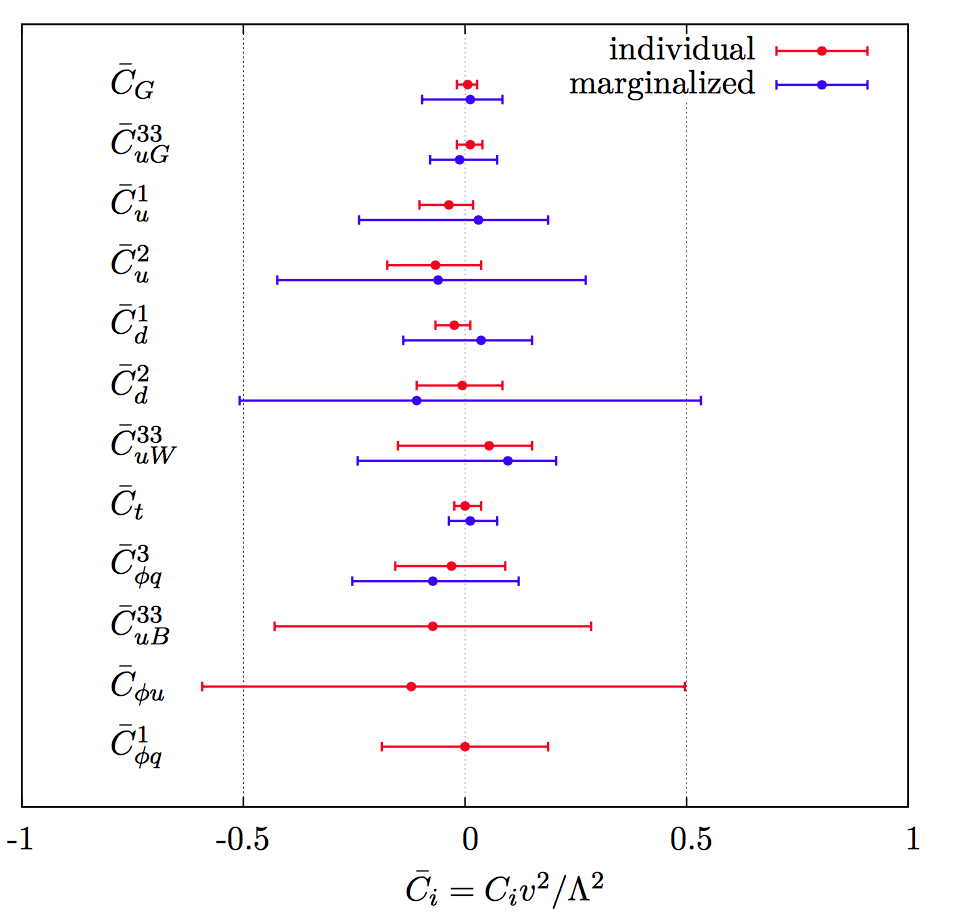
\includegraphics[width=1.0\linewidth]{1_Introduction/Figures/anomlouscouplings}
	\caption{Global fit results of top quark effective field theory to experimental data including all constrained operators at dimension six. For the operators, the Warsaw basis of~\cite{Grzadkowski:2010es} is used. The bounds are set on the Wilson coefficients of various operators contributing to top quark production and decay in two cases (red) all other coefficients set to zero, or (blue) all other co\"efficient are marginalised over. Figure taken from \cite{Buckley:2015lku}. }
	%https://arxiv.org/pdf/1512.03360.pdf conclusion section
	\label{fig:anomlouscouplings}
\end{figure}

%\section{Experimental results on the \SM\ top quark}
%\label{sec:topexp}
%In this section a selection of experimental results of measurements of the \SM\ is presented.  

%The estimations by the CMS and ATLAS collaborations of the CKM matrix element $V_{\Ptop\Pbottom}$ from single top quark measurement are given in \fig{fig:Vtb}. The most precise estimation of $V_{\Ptop\Pbottom}$ originates from a combination of $t$-channel cross section measurements at 7 and 8~\TeV\ by the CMS collaboration resulting in $|f_{\mathrm{L}}V_{\Ptop\Pbottom}| = 0.998 \pm 0.038$ (exp.) $\pm 0.016$ (theo.). Assuming the $f_{\mathrm{L}} = 1$ and $|V_{\Ptop\Pbottom}| < 1$, this result yields a limit of $|V_{\Ptop\Pbottom}| > 0.92$ at 95\% confidence level. The most recent top quark mass measurements are given in \fig{fig:lhctopmasssep2017}. The CMS combined top quark mass measurement is $m_{\Ptop} = 172.44 \pm 0.48$~\GeV\ from 7 and 8~\TeV\ data. 

%\begin{figure}[htbp]
%	\centering
%	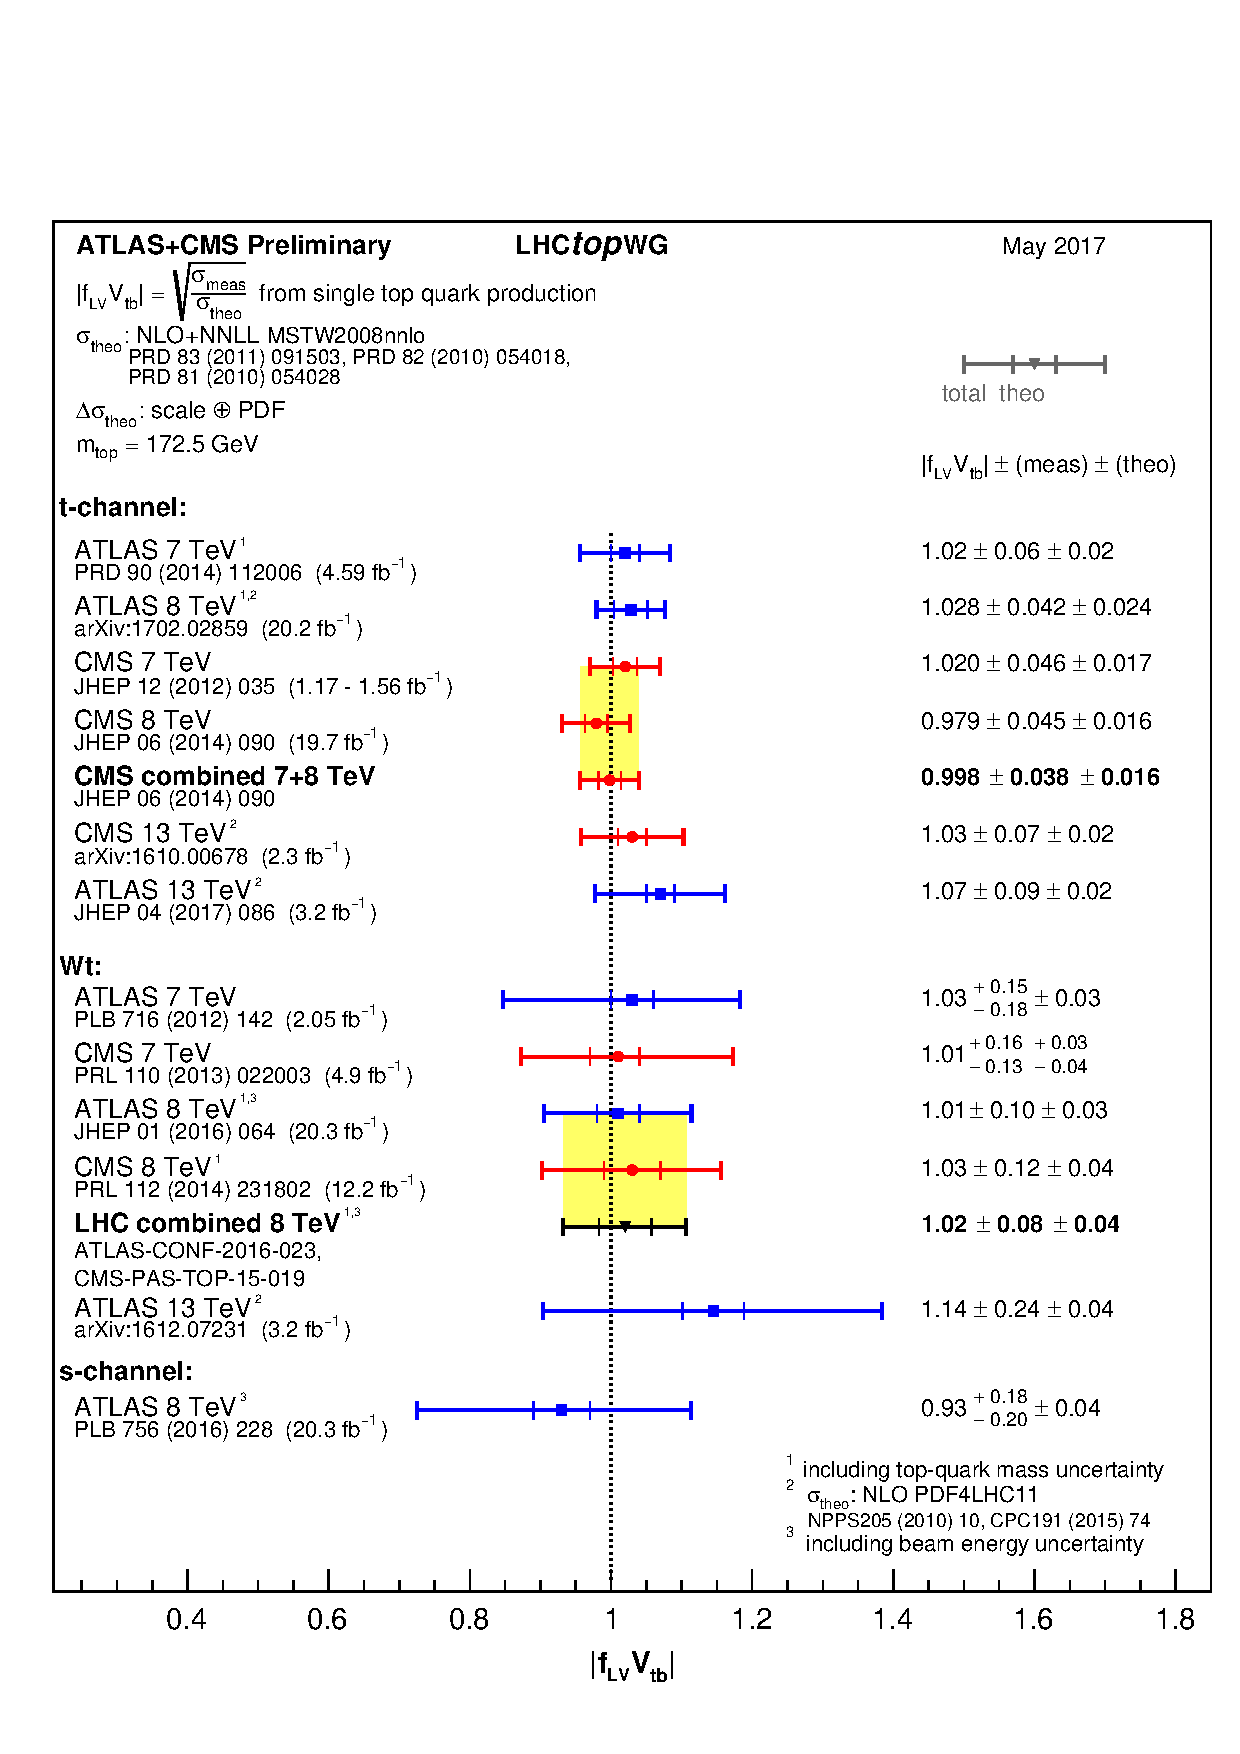
\includegraphics[width=1.\linewidth]{1_Introduction/Figures/singletop_Vtb_may2017}
%	\caption{Estimations of the \SM\ $V_{\Ptop\Pbottom}$ CKM element from single top cross section measurements. Figure taken from \cite{summarytwiki}.}
%	\label{fig:Vtb}
%\end{figure}
%\begin{figure}
%	\centering
%	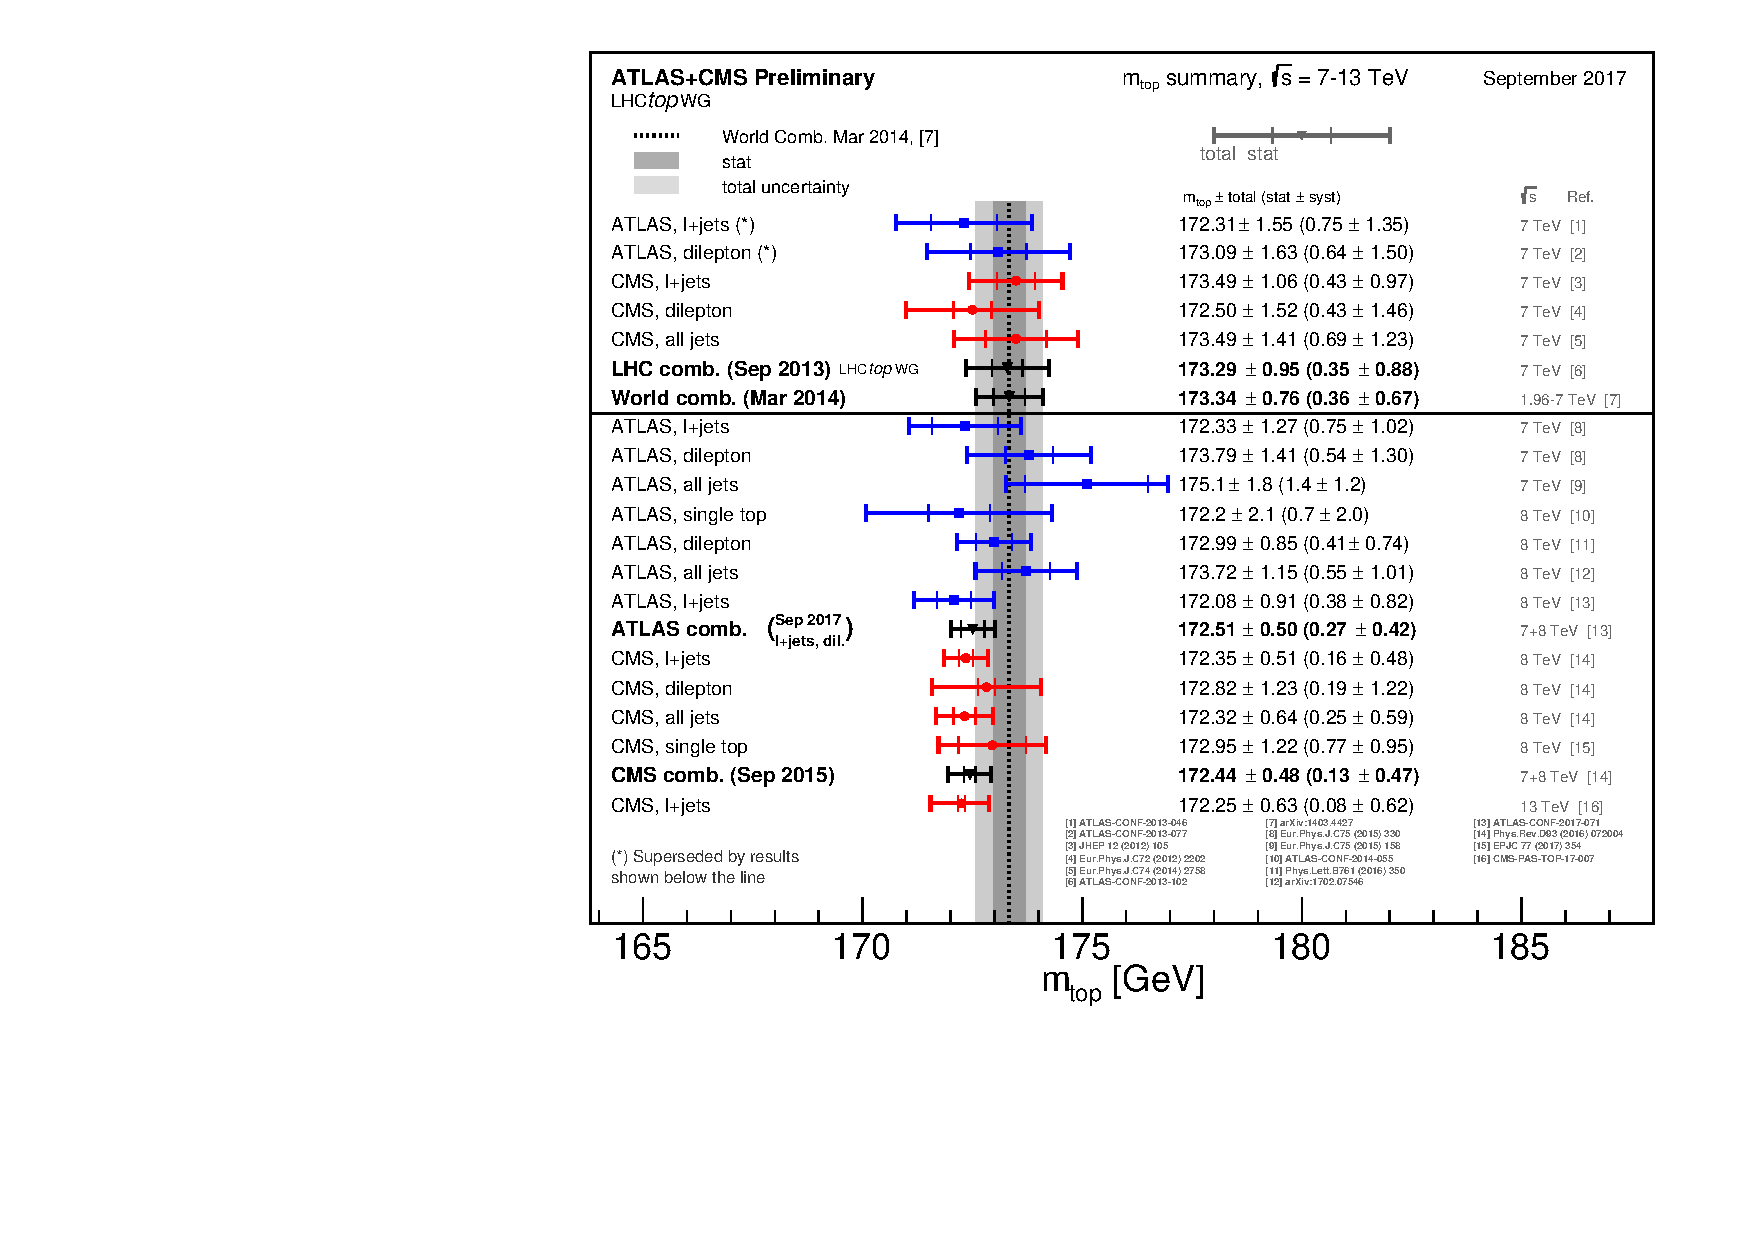
\includegraphics[width=0.7\linewidth]{1_Introduction/Figures/LHC_topmass_sep2017}
%	\caption{Summary of the top mass direct measurements performed by CMS and ATLAS, and compared with the LHC and LHC+Tevatron combinations. The results below the line are produced after the LHC and LHC+Tevatron combinations. Figure taken from \cite{summarytwiki}.}
%	\label{fig:lhctopmasssep2017}
%\end{figure}



\clearpage
\section{Motivation for new physics}
\label{sec:BSM}
Many high energy experiments confirm the success of the \SM. In particular the scalar boson, the cornerstone of the \SM, has consecrated the theory. Unfortunately there are also strong indications that the \SM\ ought to be a lower energy expression of a more global theory. The existence of physics beyond the \SM\ (BSM)~\cite{BSMWiley} is strongly motivated. These motivations are based on direct evidence from observation such as the existence of neutrino masses, the existence of dark matter and dark energy, or the matter-antimatter asymmetry, and also from theoretical problems such as the hierarchy problem, the coupling unification or the large numbers of free parameters in the \SM. 


In the \SM, the neutrinos are assumed to be massless, while experiments with solar, atmospheric, reactor and accelerator neutrinos have established that neutrinos can oscillate and change flavour during flight~\cite{Fukuda:1998mi,PhysRevLett.108.131801}. These oscillations are only possible when neutrinos have masses. The flavour neutrinos (\Pnue, \Pnum, \Pnut) are then linear expressions of the fields of at least three mass eigenstate neutrinos \Pnu$_1$, \Pnu$_2$, and \Pnu$_3$. 

The ordinary or baryonic matter described by the \SM\ describes only 5\% of the mass (energy) content of the universe. Astrophysical evidence indicated that dark matter is contributing to approximately 27\% and dark energy to 68\% of the content of the universe. From the measurements of the temperature and polarizations anisotropies of the cosmic microwave background by the Planck experiment~\cite{Ade:2015xua}, the density of cold non baryonic matter is determined. Cold dark matter is assumed to be only sensitive to the weak and gravitational force, leading to only one possible \SM\ candidate: the neutrino. However, these are too light to account for the vast amount of dark matter and other models are needed. Dark energy is assumed to be responsible for the acceleration in the expansion of the universe~\cite{Peebles:2002gy}. 
%https://en.wikipedia.org/wiki/Accelerating_expansion_of_the_universe#Evidence_for_acceleration

At the Big Bang, matter and antimatter are assumed to be produced in equal quantities. However, it  is clear that we are surrounded by matter. So where did all the antimatter go? In 1967, Sakharov identified three mechanisms that are necessary to obtain a global matter antimatter asymmetry~\cite{Sakharov}. These mechanisms are those of baryon and lepton number violation, that at a given moment in time there was a thermal imbalance for the interactions in the universe, and there is charge C and charge parity CP violation\footnote{The rate of a process $i\rightarrow f$ can be different from the CP-conjugate process: $\tilde i \rightarrow \tilde f$. The \SM\ includes sources of CP-violation through the residual phase of the CKM matrix. However, these could not account for the magnitude of the asymmetry observed.}.
% infor CP viol http://pdg.lbl.gov/2017/reviews/rpp2016-rev-cp-violation.pdf
% CP violation can occur in a filed theory when the lagrangian density involves more complex parameters than what can be removed by field redefinitions

The large number of free parameters in the \SM\ comes from the nine fermion masses, three CKM mixing angles and one CP violating phase, one EM coupling constant $g'$, one weak coupling constant $g$, one strong coupling constant $g_{\mathrm{s}}$, one QCD vacuum angle, one vacuum expectation value, and one mass of the scalar boson. This large number of free parameters leads to the expectation of a more elegant and profound theory beyond the \SM. 

The hierarchy problem~\cite{Burdman:2007ck} is related to the huge difference in energy between the weak scale and the Planck scale. The vev of the Brout-Englert-Higgs field determines the weak scale that is approximately 246~\GeV.  The radiative corrections to the scalar boson squared mass $m_{\PH}^2$, coming from its self couplings and couplings to fermions and gauge bosons, are quadratically proportional to the ultraviolet momentum cut-off $\Lambda_{\mathrm{UV}}$. This cut-off is at least equal to the energy to which the \SM\ is valid without the need of new physics. For the \SM\ to be valid up to the Planck mass, the correction to $m_{\PH}^2$ becomes thirty orders of magnitude larger than $m_{\PH}^2$. This implies that an extraordinary cancellation of terms should happen. This is also known as the naturalness problem of the \PH boson mass. 

The correction to the squared mass of the scalar boson coming from a fermion f, coupling to the scalar field $\phi$ with a coupling $\lambda_{\mathrm{f}}$ is given by
\begin{equation}
\Delta m_{\PH}^2 = -\frac{\left|\lambda_{\mathrm{f}}\right|^2}{8\pi^2}\Lambda_{\mathrm{UV}}^2, 
\end{equation}
while the correction to the mass from a scalar particle S with a mass $m_{\mathrm{S}}$, coupling to the scalar field with a Lagrangian term $-\lambda_{\mathrm{S}}|\phi|^2|\mathrm{S}|^2$ is 
\begin{equation}
\Delta m_{\PH}^2 = \frac{\left|\lambda_{\mathrm{S}}\right|^2}{16\pi^2}\left(\Lambda_{\mathrm{UV}}^2 - 2 m_{\mathrm{S}}^2 \mathrm{ln}\left(\frac{\Lambda_{\mathrm{UV}}}{m_{\mathrm{S}}}\right) + ...\right). 
\end{equation}
As one can see the correction term to $m_{\PH}^2$ is much larger than $m_{\PH}^2$ itself. By introducing BSM physics models that introduce new scalar particles at the~\TeV\ scale that couple to the scalar boson one can cancel the $\Lambda_{\mathrm{UV}}^2$ divergence and avoid this fine-tuning. 

%https://en.wikipedia.org/wiki/Hierarchy_problem
%https://www.quantumdiaries.org/2012/07/01/the-hierarchy-problem-why-the-higgs-has-a-snowballs-chance-in-hell/
%Also the large mass differences between the fermions related to the Yukawa couplings can go up to six order of magnitude in the case of the electron and the top quark and constitute the fermion mass hierarchy problem. 


The choice of the \SSU\ symmetry group itself  as well as the separate treatment of the three forces included in the \SM\ raises concern. The intensity of the forces show a large disparity around the electroweak scale, but have comparable strengths at higher energies. The electromagnetic and weak forces are unified in a electroweak interaction, but the strong coupling constant does not encounter the other coupling constants at high energies. In order to reach a grand unification, the running of couplings can be modified by the addition of new particles in \BSM\ models. 


\section{An effective approach beyond the \SM: FCNC involving a top quark}
\label{sec:EFT}
The closeness of the top quark mass to the electroweak scale led physicists to believe that it is a sensitive probe for new physics.  Studying its properties is therefore an important topic of the experimental program at the LHC. Several extensions of the \SM\ enhance the FCNC branching ratios and can be probed at the LHC~\cite{AguilarSaavedra:2004wm}, from which some of them are shown in \tab{tab:FCNCBRnp}. Previous searches have been performed at the Tevatron by the CDF \cite{PhysRevLett.101.192002} and D0 \cite{Abazov:2010qk} collaborations, 
and at the LHC by the ATLAS \cite{Aad:2015uza,Aad:2015gea,Aad:2015pja,Aaboud:2017mfd,ATLAS-CONF-2017-070} and CMS \cite{Sirunyan:2017kkr,Chatrchyan:2013nwa,Khachatryan:2015att,Sirunyan:2017kkr,Khachatryan:2016atv,CMS-PAS-TOP-17-003}  collaborations.
\begin{table}[htbp]
	\centering
	\caption{The predicted branching ratios \BR\ for FCNC interactions involving the top quark in some  \BSM\ models~\cite{AguilarSaavedra:2004wm}: quark singlet (QS), generic two Higgs doublet model (2HDM) and the minimal supersymmetric extensions to the \SM\ (MSSM);}
	\begin{tabular}{lccc|lccc}
		\toprule
		Process	& QS & 2HDM & MSSM &  Process	&  QS & 2HDM & MSSM\\ 
		\midrule
		$ \Ptop \rightarrow \Pup \PZ $     & $\leq 1.1  \times 10^{-4}$&$-$&$\leq 2  \times 10^{-6}$&$ \Ptop \rightarrow \Pcharm \PZ $      & $\leq 1.1  \times 10^{-4}$& $\leq 10^{-7}$& $\leq 2  \times 10^{-6}$\\
		$ \Ptop \rightarrow \Pup \Pphoton $& $\leq 7.5  \times 10^{-9}$&$-$&$\leq 2  \times 10^{-6}$&$ \Ptop \rightarrow \Pcharm \Pphoton $ & $\leq 7.5  \times 10^{-9}$& $\leq 10^{-6}$ &$\leq 2  \times 10^{-6}$\\
		$ \Ptop \rightarrow \Pup \Pgluon $ & $\leq 1.5  \times 10^{-7}$&$-$&$\leq 8  \times 10^{-5}$&$ \Ptop \rightarrow \Pcharm \Pgluon $  & $\leq 1.5  \times 10^{-7}$&  $\leq 10^{-4}$&$\leq 8  \times 10^{-5}$\\
		$ \Ptop \rightarrow \Pup \PHiggs $ & $\leq 4.1  \times 10^{-5}$&$\leq 5.5\;10^{-6}$&$\leq 10^{-5}$     &$ \Ptop \rightarrow \Pcharm \PHiggs $  & $\leq 4.1  \times 10^{-5}$& $\leq 10^{-3}$&$\leq 10^{-5}$\\
		\bottomrule
	\end{tabular} 
	\label{tab:FCNCBRnp}
\end{table}

The impact of \BSM\ models can be written in a model independent way by means of an effective field theory valid up to an energy scale $\Lambda$.  The leading effects are parametrized by a set of  fully gauge symmetric operators that are added to the \SM\ Lagrangian and can be reduced to a minimal set of operators as seen in \eq{eq:eft}. For simplicity, the assumption is made that new physics effects are exclusively described by dimension-6 operators, thus neglecting neutrino physics. In the fully gauge symmetric case, the EFT Lagrangian is then given by 
\begin{linenomath}
	\begin{equation}
	\Lagr_{\mathrm{SM+EFT}} = \LSM + \sum \limits_{\mathrm{i}} \frac{\bar{c}_{\mathrm{i}}}{\Lambda^2}O_{\mathrm{i}} + \order \left(\frac{1}{\Lambda^3} \right),
	\label{eq:EFTlagrangianf}
	\end{equation}
\end{linenomath}
where the Wilson coefficients $\bar{c}_{\mathrm{i}}$ depend on the considered theory and on the way that new physics couples to the \SM\ particles. Taking into account that $\Lambda$ is large, contributions suppressed by powers of $\Lambda$ greater than two are neglected. Additionally, all four fermion operators are omitted for the rest of this thesis. The Warsaw basis is adpoted for the independent effective operators~\cite{Grzadkowski:2010es}, parametrising the new physics effects relevant for the flavour changing neutral current interactions of the top quark as, all flavour indices understood, 
\begin{equation}
	\begin{aligned}
	\Lagr^{\Ptop}_{\mathrm{EFT}}  &= 
	\frac{\bar{c}_{ uG}}{\Lambda^2}
	\Phi^{\dagger} \!\cdot\!
	\left[ \bar{Q}_{\mathrm{L}} \sigma^{\mu\nu} \mathcal{T}_a u_{\mathrm{R}}\right] G^a_{\mu\nu} +
	\frac{\bar{c}_{ uB}}{\Lambda^2}
	\Phi^{\dagger} \!\cdot\!
	\left[ \bar{Q}_{\mathrm{L}} \sigma^{\mu\nu} u_{\mathrm{R}}\right] B_{\mu\nu} +
	\frac{2 \bar{c}_{ uW}}{\Lambda^2}
	\Phi^{\dagger} {T}_{\mathrm{i}} \!\cdot\!
	\left[ \bar{Q}_{\mathrm{L}} \sigma^{\mu\nu} u_{\mathrm{R}}\right] W^{\mathrm{i}}_{\mu\nu} \\
    &  +\ i \frac{\bar{c}_{ hu}}{\Lambda^2}
	\left[ \Phi^{\dagger} \overleftrightarrow{D}_\mu \Phi \right]
	\left[ \bar{u}_{\mathrm{R}} \gamma^\mu u_{\mathrm{R}}\right] 
	+ i \frac{\bar{c}_{ hq}^{(1)}}{\Lambda^2}
	\left[ \Phi^{\dagger} \overleftrightarrow{D}_\mu \Phi \right] 
	\left[ \bar{Q}_{\mathrm{L}} \gamma^{\mu} Q_{\mathrm{L}} \right] \\
	&\ +  \ i \frac{4 \bar{c}_{\PH\Pquark}^{(3)}}{\Lambda^2}
	\left[ \Phi^{\dagger} {T}_{i} \overleftrightarrow{D}_\mu \Phi \right]
	\left[ \bar{Q}_{\mathrm{L}} \gamma^\mu { T}^{\mathrm{i}} Q_{\mathrm{L}}\right]
	+  \frac{\bar{c}_{uh}}{\Lambda^2} \Phi^{\dagger}\Phi\ 
	\Phi^{\dagger} \cdot \left[ \bar{Q}_{\mathrm{L}} u_{\mathrm{R}}\right]
	+ \mathrm{ h.c.} \ ,
	\end{aligned}
	\label{eq:Wil}
\end{equation}
where the left handed \Stwo\ doublet of the quark fields is denoted by $Q_{\mathrm{L}}$, the up-type right handed fields by $u_{\mathrm{R}}$, the down-type right handed fields by $d_{\mathrm{R}}$, the \Stwo\ doublet of the Higgs field by $\Phi$, the field strength tensors as 
\begin{equation}
	\begin{aligned}
	B_{\mu\nu} &= \partial_{\mu} B_{\nu} - \partial_{\nu} B_{\mu}, \\
	W_{\mu\nu}^{\mathrm{k}} &= \partial_{\mu} W_{\nu}^{\mathrm{k}} - \partial_{\nu} W_{\mu}^{\mathrm{k}}-g\epsilon_{\mathrm{ij}}^{\mathrm{k}}W_{\mu}^{\mathrm{i}}W_{\nu}^{\mathrm{j}},\\
    	\Gtensor &= \partial_{\mu} \mathrm{G}_{\nu}^{\mathrm{a}} -  \partial_{\nu}  \mathrm{G}_{\mu}^{\mathrm{a}} + g_{\mathrm{s}} f^{\mathrm{a}}_{\mathrm{bc}}   \mathrm{G}_{\mu}^{\mathrm{b}} \mathrm{G}_{\nu}^{\mathrm{c}} , 
	\end{aligned}
\end{equation}
denoting the structure constant of the \Sthree\ group  as $f^{\mathrm{a}}_{\mathrm{bc}}$ and the structure constant of the \Stwo\ group as $\epsilon_{\mathrm{ij}}^{\mathrm{k}}$. The gauge covariant derivatives are also standard defined as 
\begin{equation}
D_{\mu} \Phi   = \partial_{\mu} \Phi - \frac{1}{2}ig'B_{\mu}\Phi - igT_{\mathrm{k}}W_{\mu}^{\mathrm{k}}\Phi
\end{equation}
with the conventions of \Sec{sec:SMlagr}. The representation matrices $T$ of \Stwo\ are defined in \eq{eq:Stwee}, while the representation matrices $\mathcal{T}$ of \Sthree\ are the Gell-Mann matrices~\cite{Peskin:257493}. The hermiatian derivative operator is defined as 
\begin{equation}
	\Phi{\dagger}\overleftrightarrow{D}\Phi = \Phi^{\dagger}D^{\mu}\Phi - D_{\mu}\Phi^{\dagger}\Phi.
\end{equation}

 After electroweak symmetry breaking,  the operators induce~\cite{AguilarSaavedra:2004wm,Beneke:2000hk} both corrections to the \SM\ couplings and new interactions at tree level such as FCNC interactions. The FCNC interactions of the top quark that are not present in the \SM\ are given by
\begin{align}
\Lagr^{\Ptop}_{\mathrm{EFT}} =\frac{\sqrt{2}}{2}\sum\limits_{\Pquark = \Pup,\Pcharm} &\left[g'
\frac{\kfqt}{\Lambda} \photontensor \APtop \sigma^{\mu\nu}\left(f^{\mathrm{L}}_{\Pphoton\Pquark} P_{\mathrm{L}} + f^{\mathrm{R}}_{\Pphoton\Pquark} P_{\mathrm{R}}\right) \Pquark \right. \\
&+ \frac{g}{2\cW} \frac{\kZqt}{\Lambda} \Ztensor \APtop \sigma^{\mu\nu}\left(f^{\mathrm{L}}_{\PZ\Pquark} P_{\mathrm{L}} + f^{\mathrm{R}}_{\PZ\Pquark} P_{\mathrm{R}}\right) \Pquark \\
&+\frac{\sqrt{2}g}{4\cW} \zZqt \APtop \gamma^{\mu} \left(\tilde{f}^{\mathrm{L}}_{\Pquark} P_{\mathrm{L}} + \tilde{f}^{\mathrm{R}}_{\Pquark} P_{\mathrm{R}}\right) \Pquark \PZ_{\mu} \\
&+ g_{\mathrm{s}} \frac{\kgqt}{\Lambda} \Ztensor \APtop \sigma^{\mu\nu}\left(f^{\mathrm{L}}_{\Pgluon\Pquark} P_{\mathrm{L}} + f^{\mathrm{R}}_{\Pgluon\Pquark} P_{\mathrm{R}}\right) \Pquark \Gtensor^{\mathrm{a}}\\
&+ \left. \eta_{\PHiggs\Pquark\Ptop} \APtop\left(\hat{f}^{\mathrm{L}}_{\Pquark} P_{\mathrm{L}} + \hat{f}^{\mathrm{R}}_{\Pquark} P_{\mathrm{R}}\right) \Pquark \PHiggs + \mathrm{h.c.}\right],
\label{eq:EFTlag}
\end{align}
where the value of the \FCNC\ couplings at scale $\Lambda$ are represented by \kZqt,\kgqt,\kfqt,\zZqt, and ${ \eta_{{\PHiggs\Pquark \Ptop}}}$. These are assumed to be real and positive, with the unit of $\GeV^{-1}$ for $\kxqt$ and no unit for $\zeta_{xqt}$ and $\eta_{\mathrm{xqt}}$. In the equation $\sigma^{{\mu \nu}}$ equals to $\frac{i}{2}\left[\gamma^{{\mu}},\gamma^{\nu}\right]$,  and the left- and right-handed chirality projector operators are denoted by $P_{\mathrm{L}}$ and $P_{\mathrm{R}}$. The electromagnetic coupling constant is denoted by $g'$, the strong interaction coupling is denoted as $g_{\mathrm{s}}$, while the electroweak interaction is parametrised by the coupling constant $g$ and the electroweak mixing angle $\theta_{\mathrm{W}}$.  The complex chiral parameters are normalized according to
$ |f_{\mathrm{xq}}^{\mathrm{L}}|^2 + |f_{\mathrm{xq}}^{\mathrm{R}}|^2 = 1 $, $|\tilde{f}_{\mathrm{q}}^{\mathrm{L}}|^2 + |\tilde{f}_{\mathrm{q}}^{\mathrm{R}}|^2 = 1$, and $|\hat{f}_{\mathrm{q}}^{\mathrm{L}}|^2 + |\hat{f}_{\mathrm{q}}^{\mathrm{R}}|^2 = 1$. In the expression for $\Lagr^{\Ptop}_{\mathrm{EFT}}$, the unitary gauge is adopted and the scalar field is expanded around its vacuum expectation value $v$ with \PHiggs being the \SM\ scalar boson. The field strength tensors of the photon \photonfield, the gluon field \Gfields, and the \PZ\ boson \Zfield\ are defined as
\begin{equation}
\begin{aligned}
	\photontensor &= \partial_{\mu} \mathrm{A}_{\nu} -  \partial_{\nu} \mathrm{A}_{\mu}, \\
	  \PZ_{\mu\nu} &= \partial_{\mu} \mathrm{Z}_{\nu} -  \partial_{\nu} \mathrm{Z}_{\mu},\: \mathrm{ and } \\
	\Gtensor &= \partial_{\mu} \mathrm{G}_{\nu}^{\mathrm{a}} -  \partial_{\nu}  \mathrm{G}_{\mu}^{\mathrm{a}} + g_{\mathrm{s}} f^{\mathrm{a}}_{\mathrm{bc}}   \mathrm{G}_{\mu}^{\mathrm{b}} \mathrm{G}_{\nu}^{\mathrm{c}}.
	\end{aligned}
\end{equation}
 Note that there are two coupling constants arising in $\Lagr^{\Ptop}_{\mathrm{EFT}}$, which is a residue of electroweak symmetry breaking. The massive \PZ\ boson will appear in both the \Zfield\ field as well as the covariant derivative, leading to an extra \PZ-vertex. 
 
 
 \newpage
 The relations between the Wilson coefficients in \eqref{eq:Wil} and the coupling strengths of the interactions in \eq{eq:EFTlag} can be derived. The 14 effective operators are mapped onto 10 free parameters providing a more minimal parametrisation of the anomalous interactions of the top quark. 
 
 
 \renewcommand{\arraystretch}{1.5}
\begin{equation}
\begin{array}{l l}
 	\kgqt f^{\mathrm{L}}_{\Pgluon\Pquark} = \frac{v}{g_{\mathrm{s}} \Lambda}
 	\left[\bar{c}_{ uG}\right]_{i3}^\ast\ ,
 	\ \   &
 	\kgqt f^{\mathrm{R}}_{\Pgluon\Pquark} \!=\! \frac{v}{g_{\mathrm{s}} \Lambda}
 	\left[\bar{c}_{ uG}\right]_{3i}\ , \\
 	%
 	\kfqt f^{\mathrm{L}}_{\Pphoton\Pquark} = \frac{v}{g' \Lambda}
 	\left[\cw \bar{c}_{ uB} - \sw \bar{c}_{ uW}\right]_{i3}^\ast\ ,
 	\ \   &
 	\kfqt f^{\mathrm{R}}_{\Pphoton\Pquark} \!=\! \frac{v}{g' \Lambda}
 	\left[\sw \bar{c}_{ uB} - \cw \bar{c}_{ uW}\right]_{3i} \ ,\\
 	%
 	\kZqt f^{\mathrm{L}}_{\PZ\Pquark} = -\frac{2 \cw v}{g \Lambda}
 	\left[\sw \bar{c}_{ uB} + \cw \bar{c}_{ uW}\right]_{i3}^\ast\ ,
 	\ \   &
 	\kZqt f^{\mathrm{R}}_{\PZ\Pquark} \!=\! -\frac{2 \cw v}{g \Lambda}
 	\left[\cw \bar{c}_{ uB} \!+\! \sw \bar{c}_{ uW}\right]_{3i} \ ,\\
 	%
 	\zZqt \tilde f^{\mathrm{L}}_{\PZ\Pquark} = - \frac{2 v^2}{\Lambda^2}
 	\left[\big(\bar{c}_{ hq}^{(1)}\!-\!\bar{c}_{ hq}^{(3)}\big)_{i3} \!+\!
 	\big(\bar{c}_{ hq}^{(1)}\!-\!\bar{c}_{ hq}^{(3)}\big)_{3i}^\ast\right]\ ,
 	\ &
 	\zZqt \tilde f^{\mathrm{R}}_{\PZ\Pquark} \!=\! - \frac{2 v^2}{\Lambda^2}
 	\left[(\bar{c}_{ hu})_{i3} + (\bar{c}_{ hu})_{3i}^\ast\right] \ ,\\
 	%
 	\eta_{\Ptop\PH\Pquark} \hat f^{\mathrm{L}}_{\PH\Pquark} = \frac{3 v^2}{2 \Lambda^2}
 	\left[\bar{c}_{ uh}\right]_{3i}^\ast\ ,
 	\ &
 	\eta_{\Ptop\PH\Pquark} \hat f^{\mathrm{R}}_{\PH\Pquark} \!=\! \frac{3 v^2}{2 \Lambda^2}
 	\left[\bar{c}_{ uh}\right]_{i3} .\\
 \end{array}
\end{equation}

 
\begin{comment}
\begin{linenomath}
	\begin{equation}
	\begin{aligned}
	\Lagr_{\mathrm{SM+EFT}} &= \sum \limits_{{\Pquark=\Pup,\Pcharm,\Ptop}} \left[ 
	\frac{\sqrt 2}{2} {g_{\mathrm{s}}} { \frac{\kgqt}{\Lambda}} \APtop \sigma^{\mu \nu} \left( {f_{{\Pgluon\Pquark}}^{\mathrm{L}}} P_{\mathrm{L}} + {f_{{\Pgluon\Pquark}}^{\mathrm{R}}}P_{\mathrm{R}}\right) \Pquark \Gtensor^{\mathrm{a}} 
	+ \frac{\sqrt 2}{2} e { \frac{\kfqt}{\Lambda}} \APtop \sigma^{\mu \nu} \left( {f_{\Pphoton \Pquark}^{\mathrm{L}}} P_{\mathrm{L}} + {f_{\Pphoton \Pquark}^{\mathrm{R}}}P_{\mathrm{R}}\right) \Pquark \photontensor  \right.\\
	&+ \frac{1}{\sqrt 2}  { \eta_{{\PHiggs\Pquark \Ptop}}} \APtop  \left( {f_{\PHiggs \Pquark }^{\mathrm{L}}} P_{\mathrm{L}} + {f_{{\PHiggs \Pquark }}}^{\mathrm{R}}P_{\mathrm{R}}\right) \Pquark \PHiggs 
	+ \frac{\sqrt 2}{4} {\frac{g}{\cW}} { \frac{\kZqt}{\Lambda}} \APtop \sigma^{\mu \nu} \left( {f_{{\PZ\Pquark}}^{\mathrm{L}}} P_{\mathrm{L}} + {f_{{\PZ\Pquark}}^{\mathrm{R}}} P_{\mathrm{R}}\right) \Pquark \Ztensor \\
	&\left. + \frac{1}{4} {\frac{g}{\cW}} { \zZqt} \APtop \gamma^{\mu} \left( {\tilde{f}_{{\PZ\Pquark}}^{\mathrm{L}}} P_{\mathrm{L}} + {\tilde{f}_{{\PZ\Pquark}}^{\mathrm{R}}}P_{\mathrm{R}}\right) \Pquark \PZ_{\mu} \right] + \mathrm{h.c.} \\
	&+ \sum \limits_{\Pquark=\Pdown,\Pstrange,\Pbottom} \left[ \frac{1}{2} {g} { \frac{\kappa_{\Ptop\PW\Pquark}}{\Lambda}} \APtop \sigma^{\mu \nu} \left( {f_{\PW \Pquark}^{\mathrm{L}}} P_{\mathrm{L}} + {f_{\PW \Pquark}^{\mathrm{R}}}P_{\mathrm{R}}\right) \Pquark \PW^+_{\mu \nu} + \frac{\sqrt 2}{4} {g} { \zWqt} \APtop \gamma^{{\mu} } \left( {\tilde{f}_{{\PW \Pquark}}^{\mathrm{L}}} P_{\mathrm{L}} + {\tilde{f}_{{\PW \Pquark}}^{\mathrm{R}}}P_{\mathrm{R}}\right) \Pquark \PW^+_{{\mu}} \right] \\ 
	&+ \mathrm{h.c.} , 
	\end{aligned}
	\label{eq:EFTlagrangianexpanded}
	\end{equation}
\end{linenomath}
where the value of the \FCNC\ couplings at scale $\Lambda$ are represented by \kZqt,\kgqt,\kfqt,\zZqt, and ${ \eta_{{\PHiggs\Pquark \Ptop}}}$. These are assumed to be real and positive, with the unit of $\GeV^{-1}$ for $\kxqt$ and no unit for $\zeta_{xqt}$ and $\eta_{\mathrm{xqt}}$. In the equation $\sigma^{{\mu \nu}}$ equals to $\frac{i}{2}\left[\gamma^{{\mu}},\gamma^{\nu}\right]$,  and the left- and right-handed chirality projector operators are denoted by $P_{\mathrm{L}}$ and $P_{\mathrm{R}}$. The electromagnetic coupling constant is denoted by $e$, the strong interaction coupling is denoted as $g_{\mathrm{s}}$, while the electroweak interaction is parametrised by the coupling constant $g$ and the electroweak mixing angle $\theta_{\mathrm{W}}$.  The complex chiral parameters and are assumed to be real  and  fulfil the relation 
$ \left(|f_{\mathrm{xq}}^{\mathrm{L}}|^2 + |f_{\mathrm{xq}}^{\mathrm{R}}|^2 \right)= 1 $ and $\left(|\tilde{f}_{\mathrm{xq}}^{\mathrm{L}}|^2 + |\tilde{f}_{\mathrm{xq}}^{\mathrm{R}}|^2 \right)= 1$.
% The limitations of the electro weak broken phase approach are summarised in \cite{Durieux:2014xla}. 

\end{comment}

\section{Experimental constraints on top-FCNC}
\label{sec:ExpConstr}
Experiments commonly put limits on the branching ratios which allow an easier interpretation across different EFT models by use of the branching ratio
\begin{equation}
	\BR(\Ptop \rightarrow \Pquark\mathrm{X}) = \frac{\delta^2_{\Ptop \mathrm{X}\Pquark}\Gamma_{\Ptop \rightarrow \Pquark\mathrm{X}}}{\Gamma_{\Ptop}},
\end{equation}
where $\Gamma_{\Ptop \rightarrow \Pquark\mathrm{X}}$ represents the \FCNC\ decay width\footnote{The decay width of a certain process represents the probability per unit time that a particle will decay. The total decay width, defined as the sum of all possible decay widths of a particle, is inversely proportional to its lifetime. } for a coupling strength $\delta^2_{\Ptop \mathrm{X}\Pquark}=1$, and $\Gamma_{\Ptop}$ the full decay width of the top quark. In the \SM, supposing a top quark mass of 172.5~\GeV, the full width becomes $\Gamma_{\Ptop}^{\mathrm{SM}} = 1.32$~\GeV~\cite{Gao:2012ja}. 

% top FCNC vertex in Feynman diagram -> matrix element maal kappa --> cross sectie maal kappa^2 --> cross sectie maal BR (lineair)


Searches for top-FCNC usually adopt a search strategy depending on the experimental set-up and the FCNC interaction of interest,  looking either for \FCNC\ interactions in the production of a single top quark or in its decay for top quark pair interactions. In \fig{fig:Feynman}, these two cases are shown for the \tZq\ vertex.  \\
\begin{figure}[hbtp]
	\centering
	\subbottom[]{
			\begin{fmffile}{singletop}
		\begin{fmfgraph*}(160,40) % width - height
\fmfleft{i1,i2} 
\fmfright{o1,o2}
 \fmf{fermion}{i1,v1,v2,o2}
  \fmf{boson}{v2,o1}
   \fmf{gluon}{i2,v1}
   \fmflabel{\Pgluon}{i2}
   \fmflabel{\Pup,\Pcharm}{i1}
   	\fmfv{label= ,decor.shape=circle,decor.filled=shaded,decor,size=0.5thick, label.angle=-90}{v2}
  % \fmflabel{\Pup,\Pcharm}{i1}
   \fmflabel{\PZ}{o1}
   \fmflabel{\Ptop}{o2}
    \fmf{fermion,label=\Pup,,\Pcharm,label.dist=10}{v1,v2}
      \end{fmfgraph*}
\end{fmffile}
}
\hspace*{1cm}
\subbottom[]{
	\begin{fmffile}{toppair}
	\begin{fmfgraph*}(160,40) % width - height
		\fmfleft{i1,i2} 
		\fmfright{o1,o2,o3,o4}
		\fmflabel{\Pgluon}{i1}
		\fmflabel{\Pgluon}{i2}
		\fmflabel{\APup,\APcharm}{o1}
		\fmflabel{\PZ}{o2}
		\fmflabel{\PWp}{o3}
		\fmflabel{\Pbottom}{o4}
		\fmf{gluon}{i1,v1,i2}
		\fmf{gluon,label=\Pgluon,label.dist=10}{v1,v2}
		\fmf{fermion}{o1,v4,v2,v3,o4}
		\fmffreeze
		\fmf{boson}{v3,o3}
		\fmf{boson}{v4,o2}
		\fmfv{label= ,decor.shape=circle,decor.filled=shaded,decor,size=0.2thick, label.angle=-90}{v4}
		 \fmf{fermion,label=\Ptop,label.dist=5}{v2,v3}
		 \fmf{fermion,label=\APtop,label.dist=-20}{v4,v2}
		\fmflabel{}{v3}
		\fmflabel{}{v2}
		\fmflabel{}{v1}
	\end{fmfgraph*}
\end{fmffile}
}
\caption{Feynman diagrams for the processes with a \tZq\ \FCNC\ interaction, where the FCNC interaction is indicated with the shaded dot. (a) Single top quark production through an \FCNC\ interaction. (b) Top quark pair production with an \FCNC\ induced decay. }
\label{fig:Feynman}
\end{figure}


The observation of top-FCNC interactions has yet to come and experiments have so far only been able to put upper bounds on the branching ratios. An overview of the best current limits is given in \tab{tab:FCNClimits}. In \fig{fig:fcncupperlimits} a comparison is shown between the current best limits set by ATLAS and CMS with respect to several \BSM\ model benchmark predictions. From there one can see that \FCNC\ searches involving a \PZ\ or \PHiggs\ boson are close to excluding or confirming several \BSM\ theories. In \fig{fig:summaryfcnc}, the searches performed by CMS are summarised. For the tZq vertex, the best limit from CMS comes from Ref. \cite{Sirunyan:2017kkr} where both single top quark and top quark pair are studied. The observed (expected) limits 95\% CL at 8 \TeV\ for the FCNC tZq interaction by CMS are $\BR(\Ptop \rightarrow \Pup\PZ) <  2.2 \times 10^{-4} (2.7  \times 10^{-4})$ and  $\BR(\Ptop \rightarrow \Pcharm\PZ) < 4.9 \times 10^{-4} (12 \times 10^{-4})$. In \fig{fig:FCNCATLASCMS}, the summary of the 95\% confidence level observed limits on the branching ratios of the top quark decays to a charm or up quark and a neutral boson is given, considering the results from the HERA, the LEP, the Tevatron, and the LHC.
\begin{table}[htbp]
	\centering
	\caption{Overview of the most stringent observed and expected experimental limits on top-FCNC branching ratios \BR\ at 95\% confidence level.}
	\begin{tabular}{llllll}
		\toprule
		Process &Search mode & Observed \BR & Expected \BR & \multicolumn{2}{c}{Experiment} \\ 
		\midrule
%		$\Ptop \rightarrow \Pup\PZ$		     & \tt\ decay  and \st\ production & 2.2 $\times 10^{-4}$& 2.7 $\times 10^{-4}$   & CMS&\cite{Sirunyan:2017kkr}\\
        $\Ptop \rightarrow \Pup\PZ$		     & \tt\ decay   & 1.7 $\times 10^{-4}$& 2.4 $\times 10^{-4}$   & ATLAS&\cite{ATLAS-CONF-2017-070} \\
		$\Ptop \rightarrow \Pup\Pphoton$	 & \st\ production   & 1.3 $\times 10^{-4}$& 1.9 $\times 10^{-4}$& CMS&\cite{Khachatryan:2015att}     \\
		$\Ptop \rightarrow \Pup\Pgluon$		 & \st\ production   & 4.0   $\times 10^{-5}$& 3.5   $\times 10^{-5}$& ATLAS&\cite{Aad:2015gea}   \\
		$\Ptop \rightarrow \Pup\PHiggs$		 & \tt\ decay        & 2.4 $\times 10^{-3}$& 1.7 $\times 10^{-3}$& ATLAS&\cite{Aaboud:2017mfd}   \\
%		$\Ptop \rightarrow \Pcharm\PZ$		 & \tt\ decay  and \st\ production        & 4.9 $\times 10^{-4}$& 12  $\times 10^{-4}$& CMS&\cite{Sirunyan:2017kkr}\\
        $\Ptop \rightarrow \Pcharm\PZ$		 & \tt\ decay        & 2.3 $\times 10^{-4}$& 3.2  $\times 10^{-4}$& ATLAS&\cite{ATLAS-CONF-2017-070}\\
		$\Ptop \rightarrow \Pcharm\Pphoton$  & \st\ production   & 2.0 $\times 10^{-3}$& 1.7 $\times 10^{-3}$& CMS&\cite{Khachatryan:2015att}     \\
		$\Ptop \rightarrow \Pcharm\Pgluon$   & \st\ production   & 2.0   $\times 10^{-4}$& 1.8 $\times 10^{-4}$& ATLAS&\cite{Aad:2015gea}   \\
		$\Ptop \rightarrow \Pcharm\PHiggs$   & \tt\ decay     & 2.2  $\times 10^{-3}$& 1.6 $\times 10^{-3}$& CMS&\cite{Aaboud:2017mfd}     \\
		\bottomrule
	\end{tabular} 
	\label{tab:FCNClimits}
\end{table}

\begin{figure}[htbp]
	\centering
	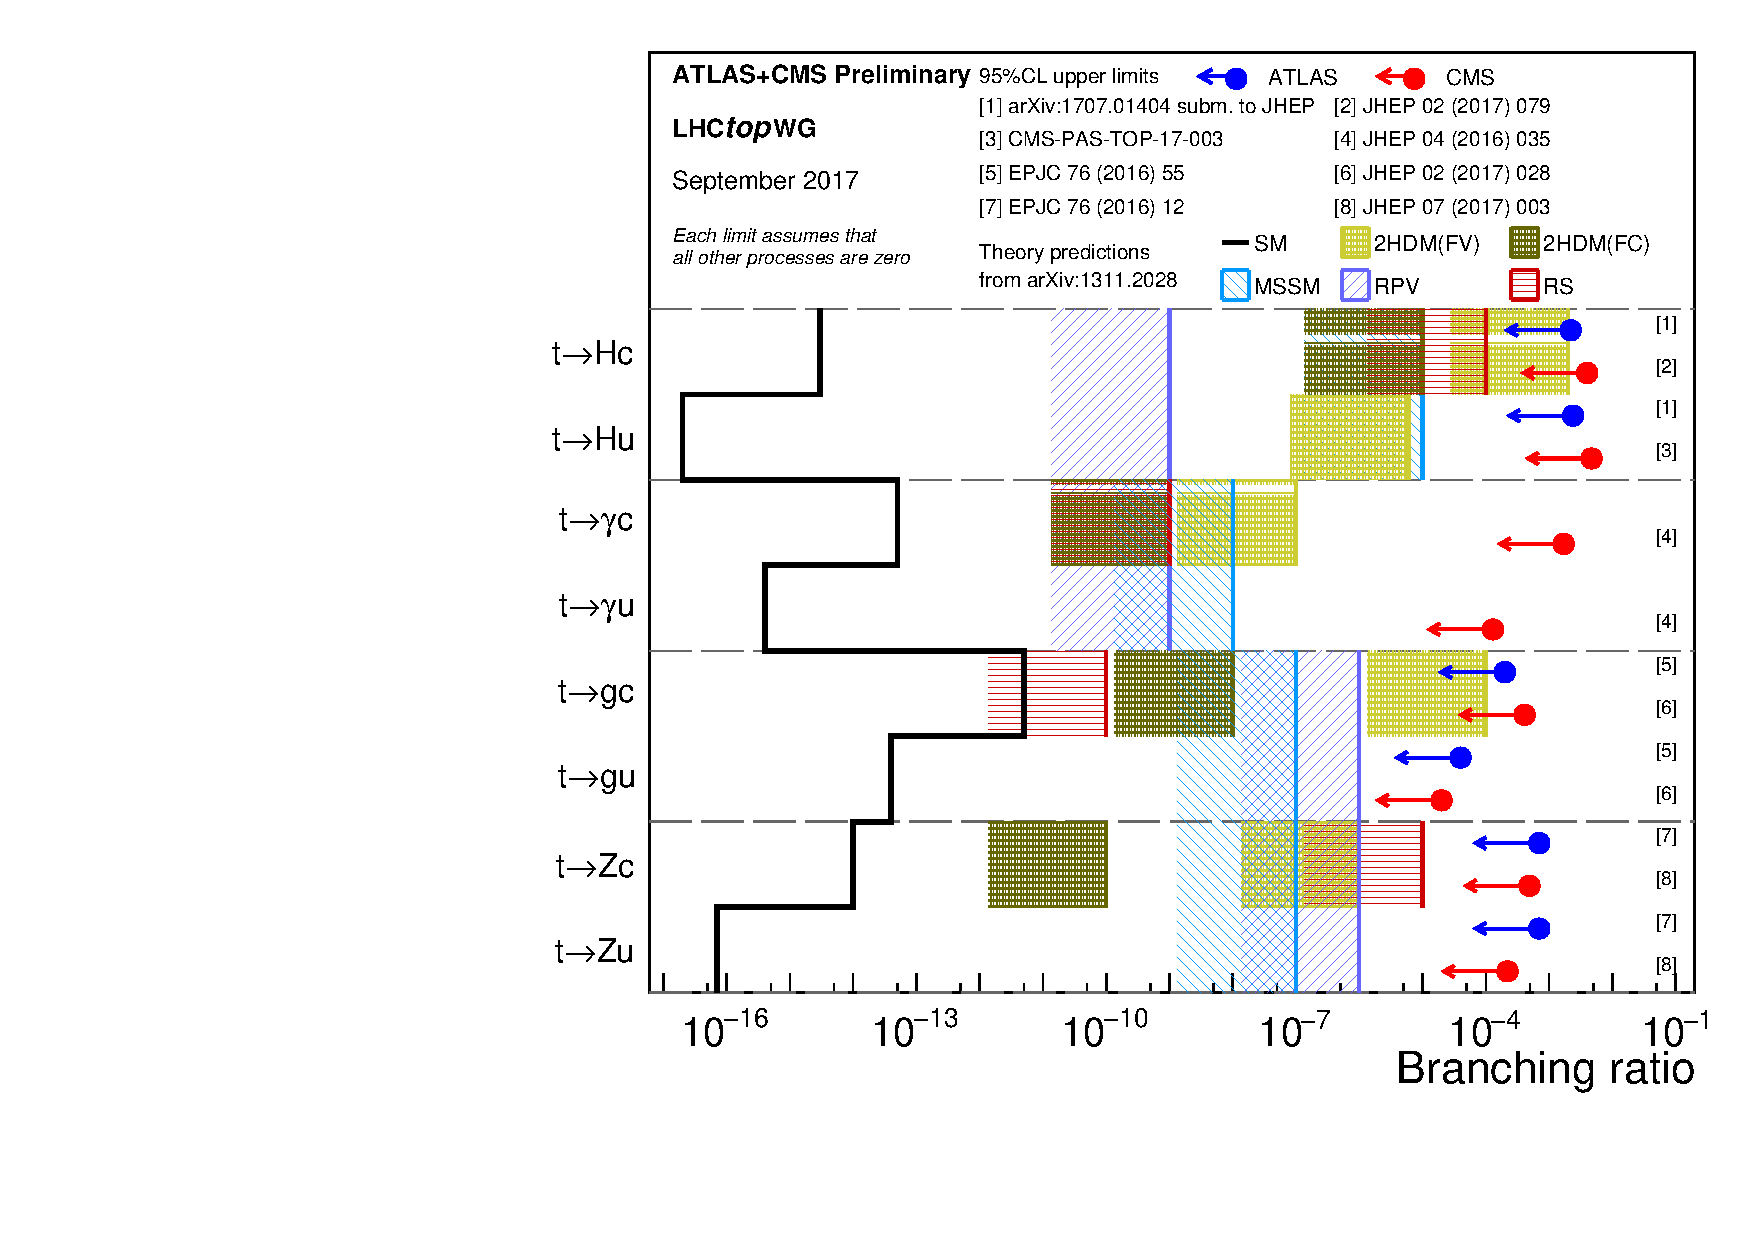
\includegraphics[width=0.7\linewidth]{1_Introduction/Figures/fcnc_summarybsm_sep17.pdf}
	\caption{Current best limits set by CMS and ATLAS for top-FCNC interactions.  Figure taken from \cite{summarywiki}. (TO DO Remake with new atlas results)}
	\label{fig:fcncupperlimits}
\end{figure}
\begin{figure}[htbp]
	\centering
	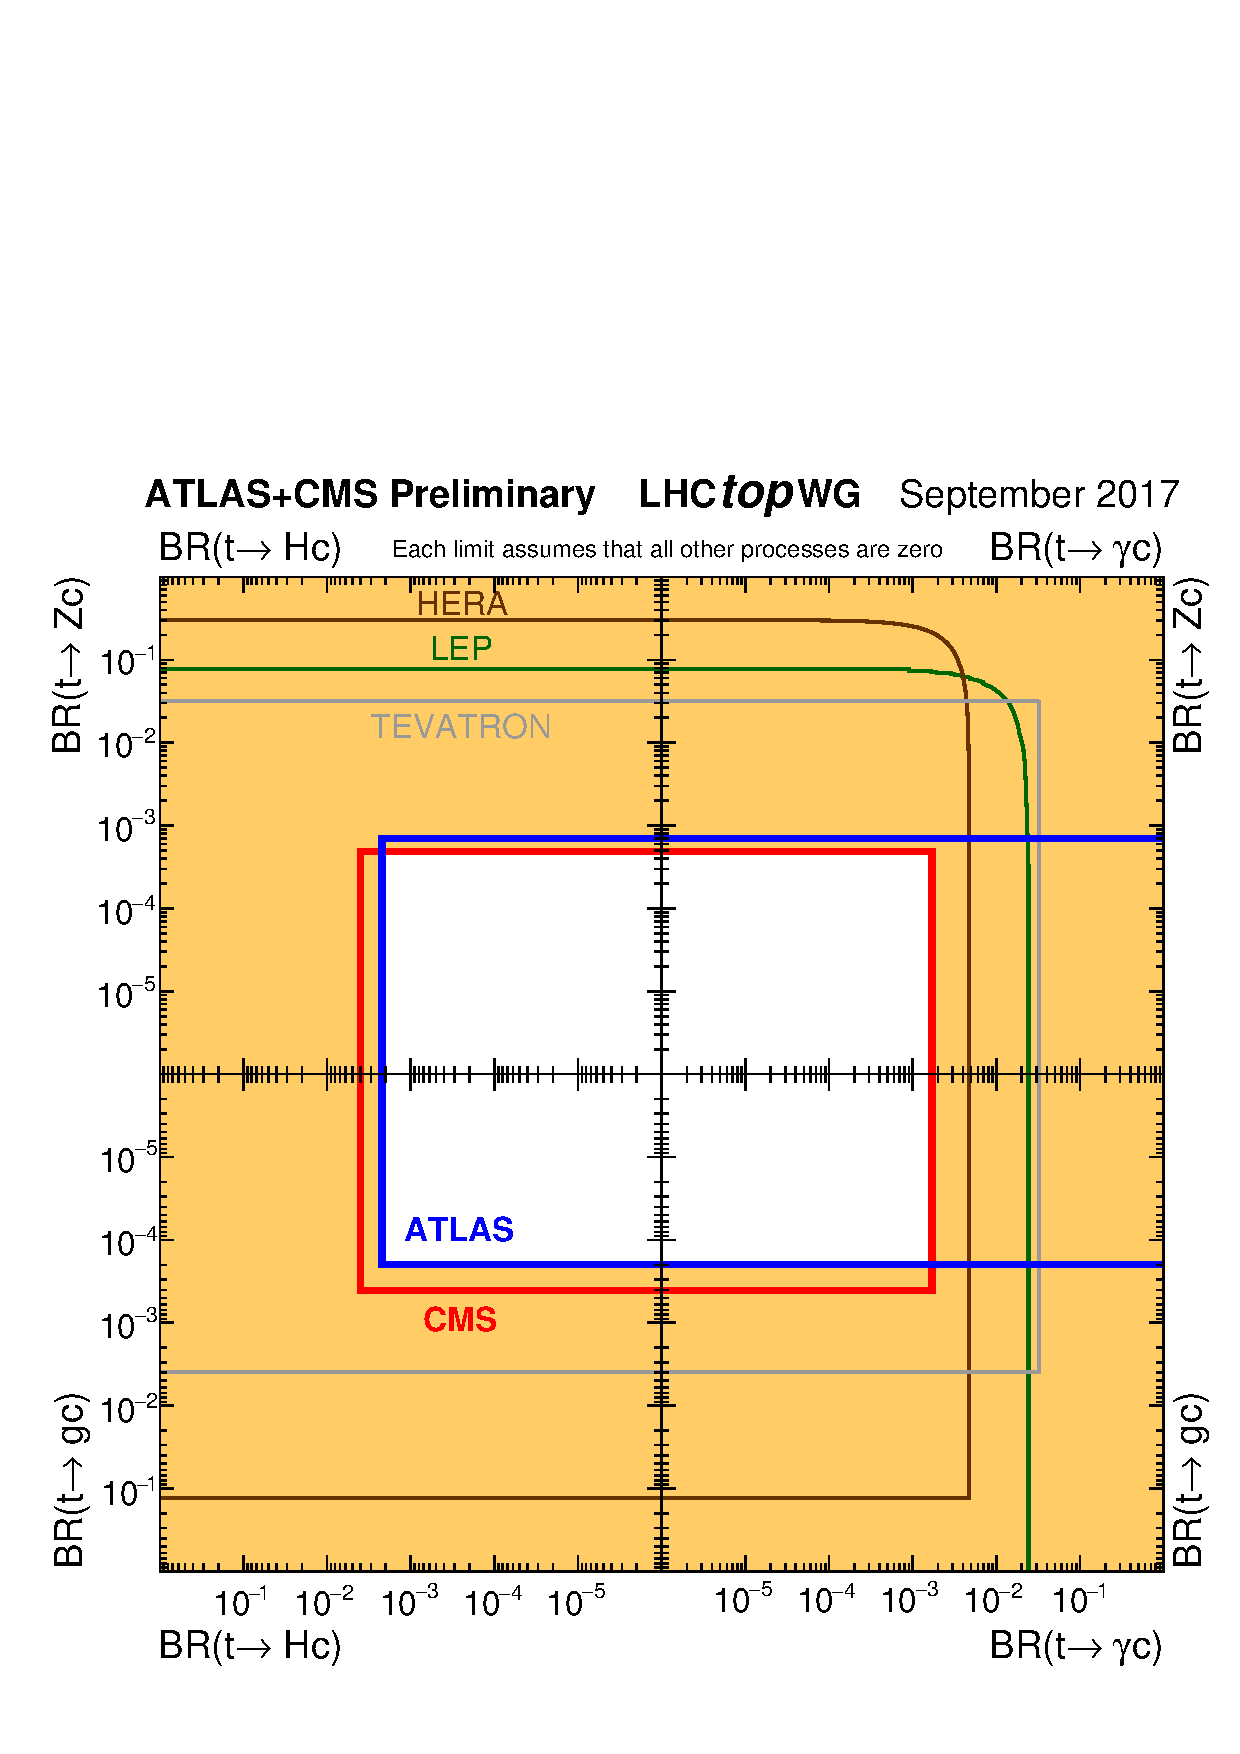
\includegraphics[width=0.49\linewidth]{1_Introduction/Figures/fcnc_tXc_sep17.pdf}
	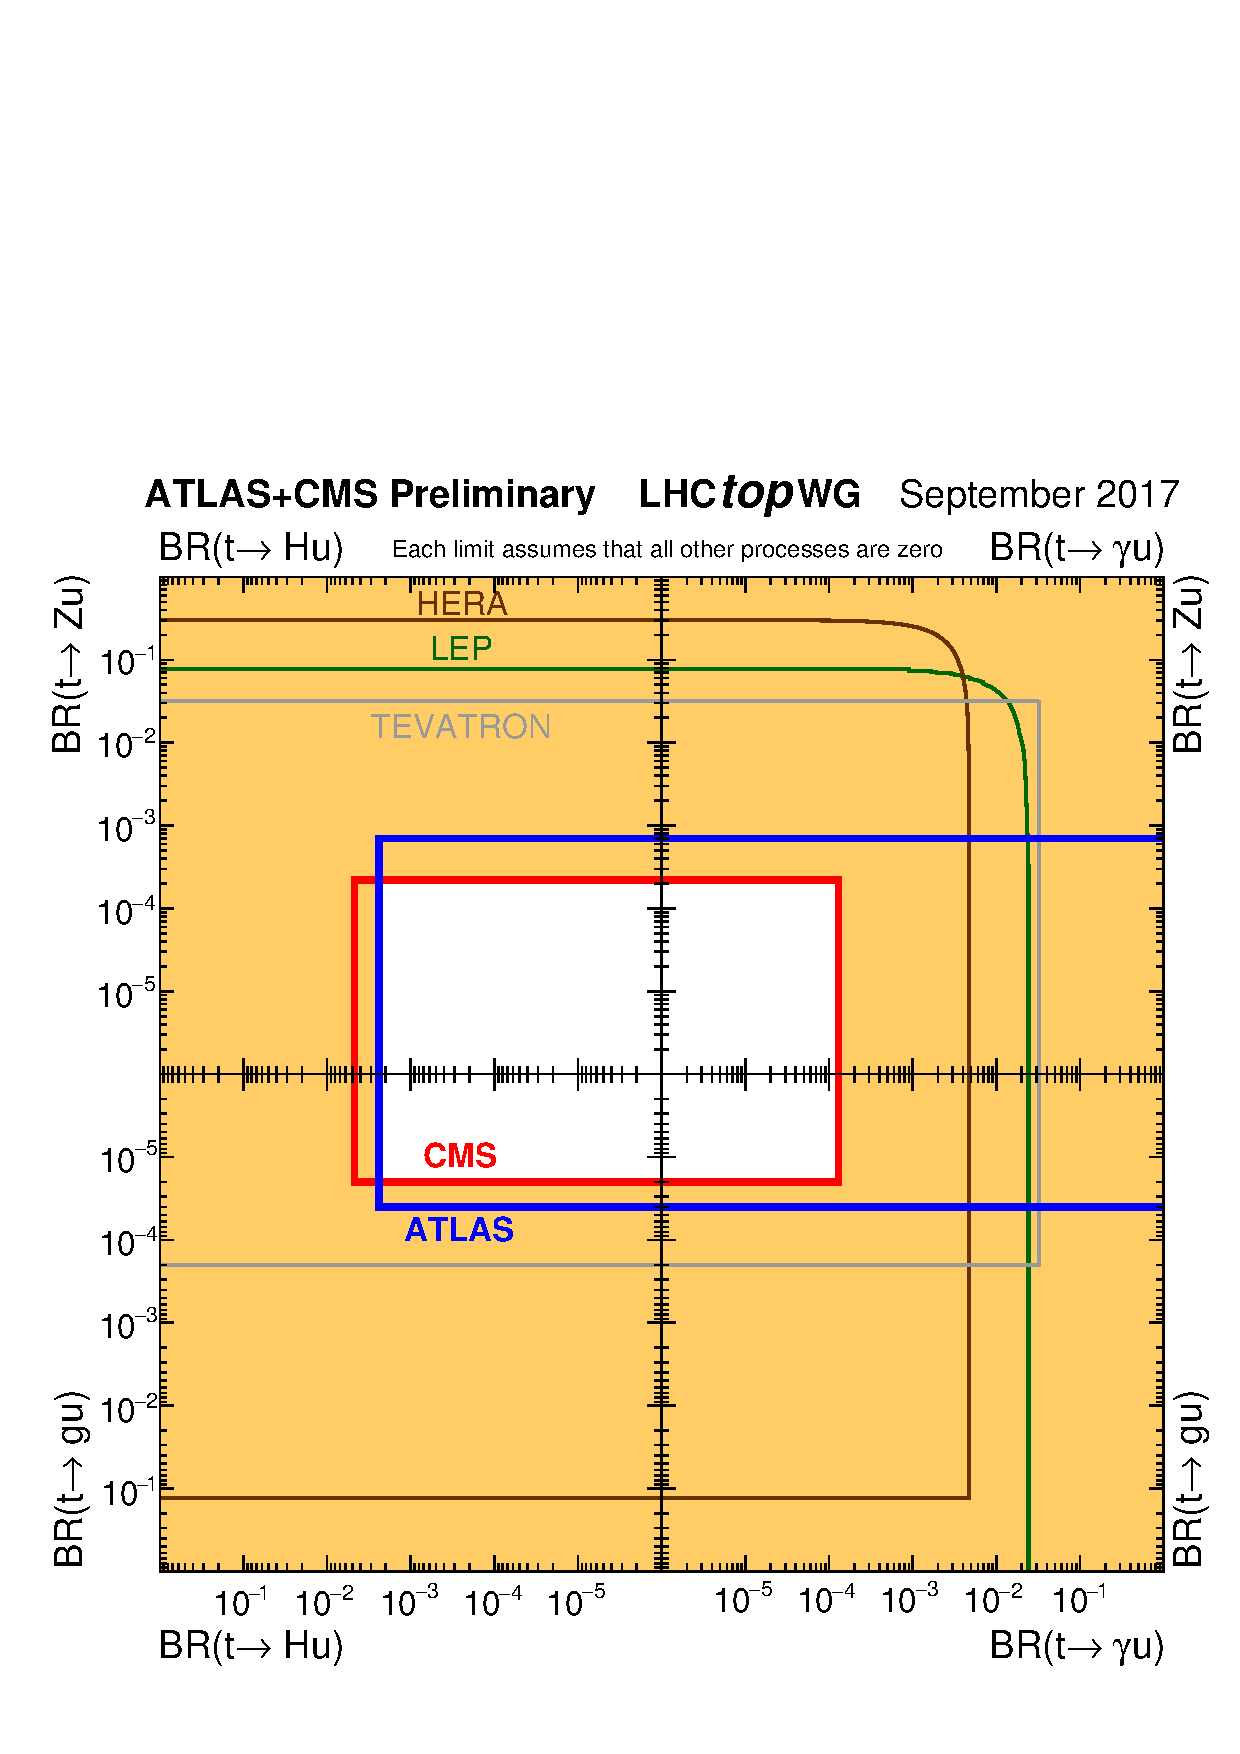
\includegraphics[width=0.49\linewidth]{1_Introduction/Figures/fcnc_tXu_sep17.pdf}
	\caption{Summary of the current 95\% confidence level observed limits on the branching ratios of the top quark decays via flavour changing neutral currents to a charm (left) or up (right) quark and a neutral boson. The coloured lines represent the results from HERA (the most stringent limits between the ones obtained by the H1 and ZEUS collaborations, in brown), LEP (combined ALEPH, DELPHI, L3 and OPAL collaborations result, in green), TEVATRON (the most stringent limits between the ones obtained by the CDF and D0 collaborations, in grey). The yellow area represents the region excluded by the ATLAS and the CMS Collaborations. Figure taken from \cite{summarytwiki}.}
	\label{fig:FCNCATLASCMS}
\end{figure}
\begin{figure}[htbp]
	\centering
	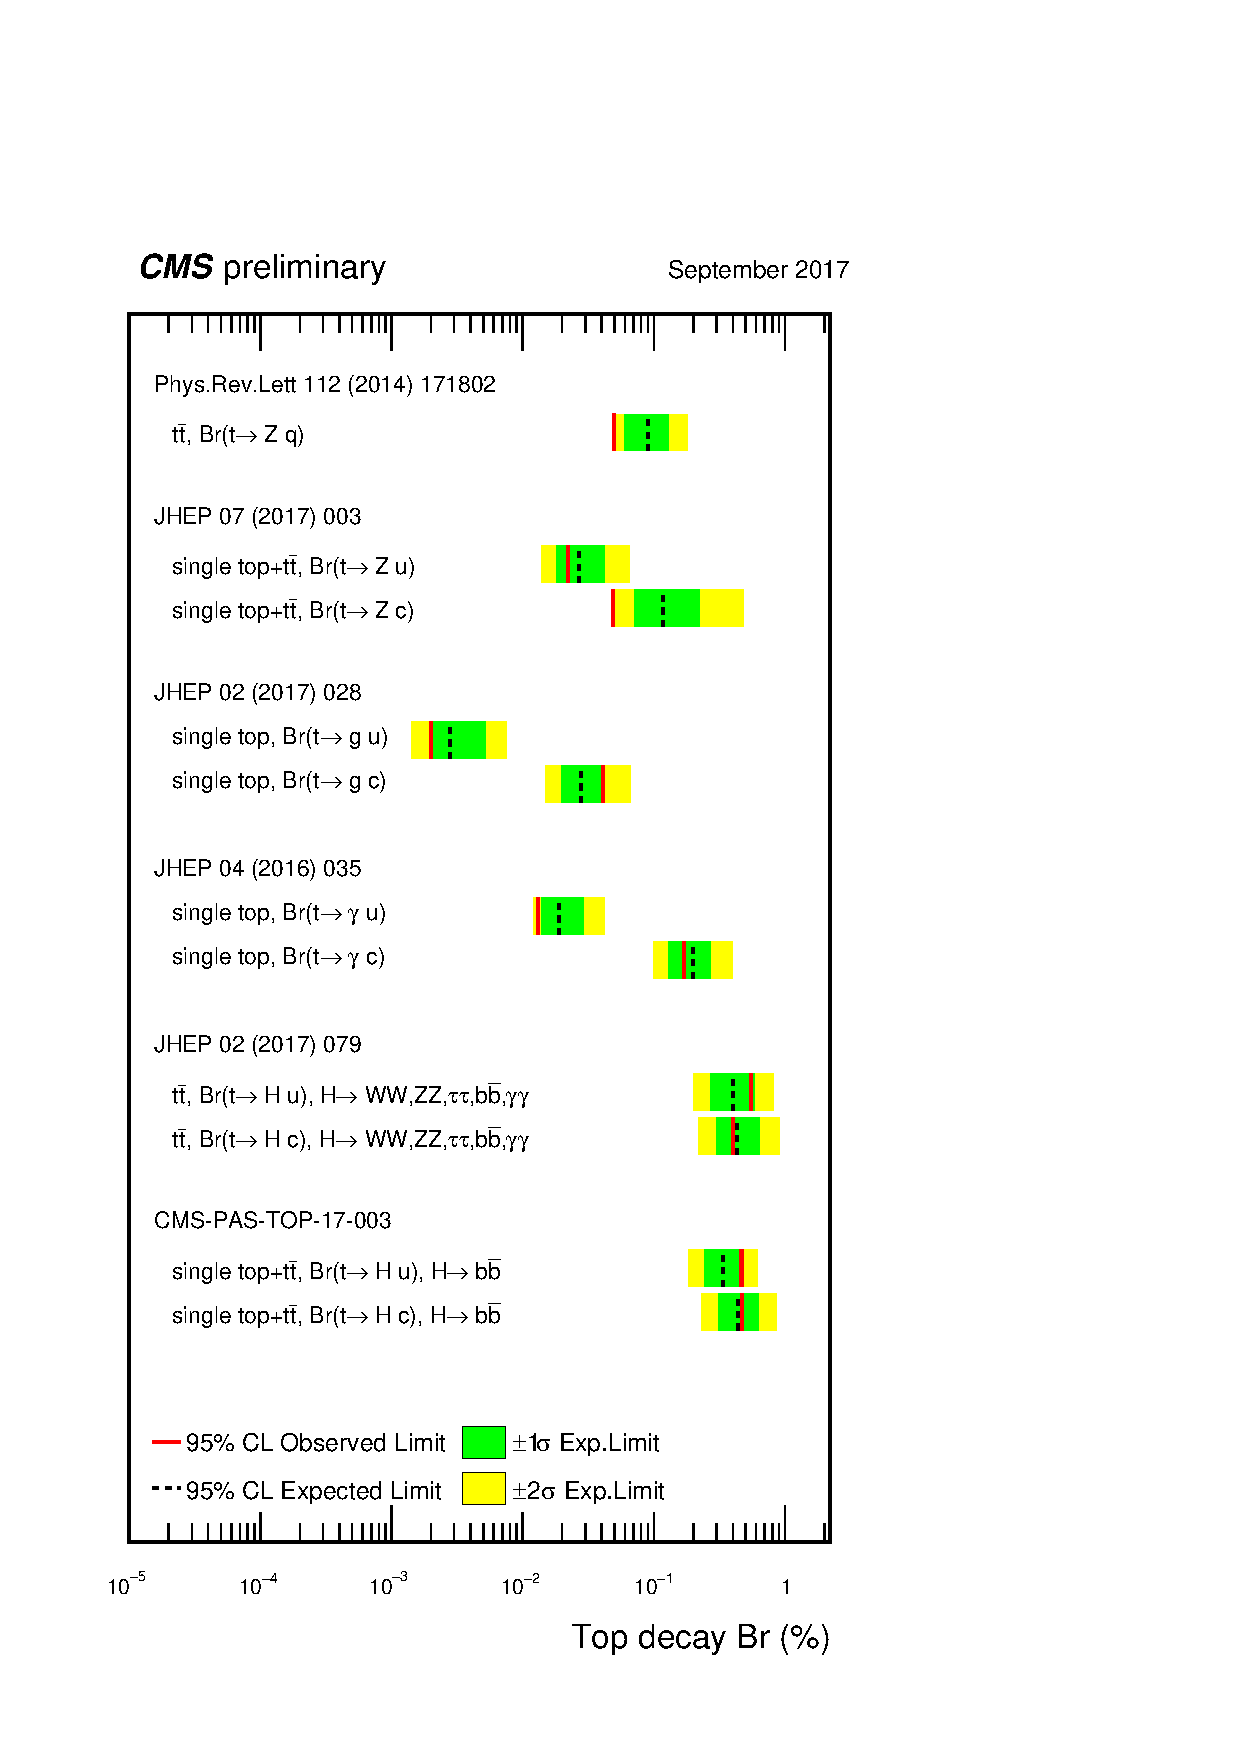
\includegraphics[width=.7\linewidth]{1_Introduction/Figures/summary_FCNC.pdf}
	\caption{Summary of the FCNC branching ratios from CMS searches at 8 \TeV. Figure taken from \cite{summarywiki}.}
	\label{fig:summaryfcnc}
\end{figure}









\chapter{Experimental set-up}
\label{chap:2}
%\epigraph{The LHC rose from the dead on Easter. I've heard thats been done before... There is a place in human knowledge where here be dragons. That is the place where the ship that is the LHC  will be going.}
%	{\textit{Don Lincoln, tedX}}


A key objective of the Large Hadron Collider (LHC) was the search for the Brout-Englert-Higgs boson. The Large  Electron Positron (LEP)~\cite{Myers:226776} and Tevatron~\cite{1748-0221-6-08-T08001} experiments established that the mass of the scalar boson has to be larger than 114 \GeV~\cite{Barate:2003sz,Herner:2016woc}, and smaller than approximate 1 \TeV\ due to unitarity and perturbativity constraints~\cite{Djouadi:2005gi}. On top of this, the search for new physics such as supersymmetry or the understanding of dark matter were part of the motivation for building the LHC. 
Since the start of its operation, the LHC is pushing the boundaries of the Standard Model, putting the most stringent limits on physics beyond the Standard Model as well as precision measurements of the parameters of the Standard Model. A milestone of the LHC is the discovery of the scalar boson in 2012 by the two largest experiments at the LHC~\cite{Chatrchyan:2012xdj,Aad:2012tfa}.

This chapter is dedicated to the experimental set-up of the LHC and the Compact  Muon Solenoid (CMS) experiment. \Sec{sec:LHC} describes the LHC and its acceleration process for protons to reach their design energies. The CMS experiment and its components are presented in \Sec{sec:CMS}. The upgrades performed during the long shutdown in 2013 are discussed in \Sec{sec:Phase1}. The data acquisition of CMS is presented in \Sec{sec:DAQ}, while the CMS computing model is shown in \Sec{sec:Computing}.


\section{The Large Hadron Collider}
\label{sec:LHC}
The LHC has started its era of cutting edge science on 10 September 2008~\cite{LHC:2008} after approval by the European Organisation of Nuclear Research (CERN) in 1995~\cite{Pettersson:291782}. Installed in the previous LEP tunnel, the LHC consists of a 26.7~\km\ quasi ring, that is installed between 45 and 170~\m\ under the French-Swiss border amidst Cessy (France) and Meyrin (Switzerland). Built to study rare physics phenomena at high energies, the LHC  can accelerate mainly two types of particles, protons and lead ions Pb$^{45+}$, and provides collisions at four interaction points, where the particle bunches are crossing. Experiments for studying the collisions are installed at each interaction point. 

 As can be seen in \fig{fig:LHCchain}, the LHC is the last element in a chain that creates, injects and accelerates protons. The starting point is the ionisation of hydrogen, creating protons that are injected in a linear accelerator (LINAC 2). Here, the protons obtain an energy of 50~\MeV. They continue to the Proton Synchrotron Booster (PSB or Booster), where the packs of protons are accelerated to 1.4~\GeV\ and each pack is split up in twelve bunches with 25 or 50~\nano\s\ spacing. The Proton Synchrotron (PS) then increases their energy to 25~\GeV\ before the Super Proton Synchrotron (SPS) increases the proton energy up to 450~\GeV. Each accelerator ring expands in radius in order to reduce the energy loss of the protons by synchrotron radiation\footnote{This energy loss is proportional to the fourth power of the proton energy and inversely proportional to the bending radius.}. Furthermore, the magnets responsible for the bending of the proton trajectories have to be strong enough to sustain the higher proton energy. Ultimately, the proton bunches are injected into opposite directions into the LHC, where they are accelerated to 3.5 \TeV\ (in 2010 and 2011), 4~\TeV\ (in 2012 and 2013) or 6.5~\TeV\ (in 2015 and 2016)~\cite{Wenninger:2254678}. 
  \begin{figure}[h]
 	\centering
 	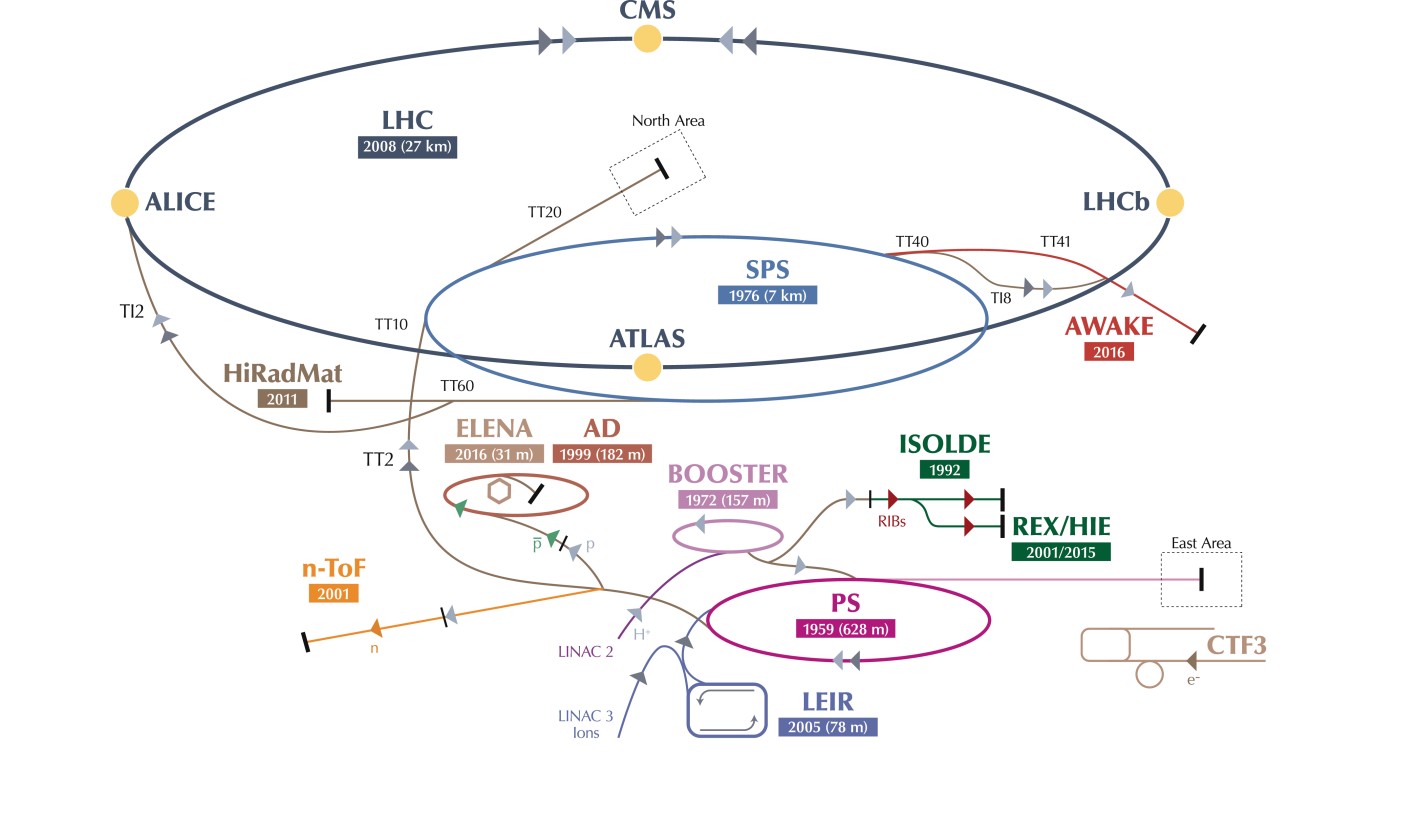
\includegraphics[width=1.\textwidth]{2_ExperimentalSetup/Figures/CCC-v2016}
 	\caption{Schematic representation of the accelerator complex at CERN~\cite{DeMelis:2197559}. The LHC (dark blue) is the last element in chain of accelerators. Protons are successively accelerated by LINAC 2, the Booster, the Proton Synchrotron (PS) and the Super Proton Synchrotron (SPS) before entering the LHC.}
 	\label{fig:LHCchain}
 \end{figure}

In \fig{fig:lhcschedule} the LHC programme is shown. the first data collisions, so-called Run 1 period, lasted from 2008 until 16 February 2013 after which  the CERN accelerator complex shut down for two years of planned maintenance and consolidation during so-called long shutdown 1 (LS1). On 23 March 2015, the new data taking period known as Run 2 started. With a brief end of the year extended technical stop (EYETS). The main activities carried out during the EYETS were the maintenance of systems such as the cryogenics, the cooling, electrical systems, etc.; the replacement of the magnet, as well as a de-cabling and cabling campaign on the SPS\cite{MurilloQuijada:2017agx}. Run 2 will last until July 2018 when the  long shutdown 2 (LS2) will begin for 2 years. The main goal of this shutdown is the LHC injectors upgrade (LUI), but also maintenance and consolidation will be performed. Furthermore, preparations for the High Luminosity LHC, which will start in 2024, will be done. More information about phase 1 upgrades during LS1 and EYETS is given in \Sec{sec:Phase1}.\\ %https://home.cern/cern-people/updates/2017/01/eyets-report-so-far-so-good\
 Before the start of the LHC in 2010, the previous energy record was held by the Tevatron collider at Fermilab, colliding protons with antiprotons at \com = 1.96~\TeV.  When completely filled, the LHC nominally contains 2220 bunches in Run 2, compared to 1380 in Run 1 (design: 2200). 
%At full intensity, it would have nearly 2800 bunches but this is limited due to a problem with SPS in 2016.
\begin{figure}[htbp]
	\centering
	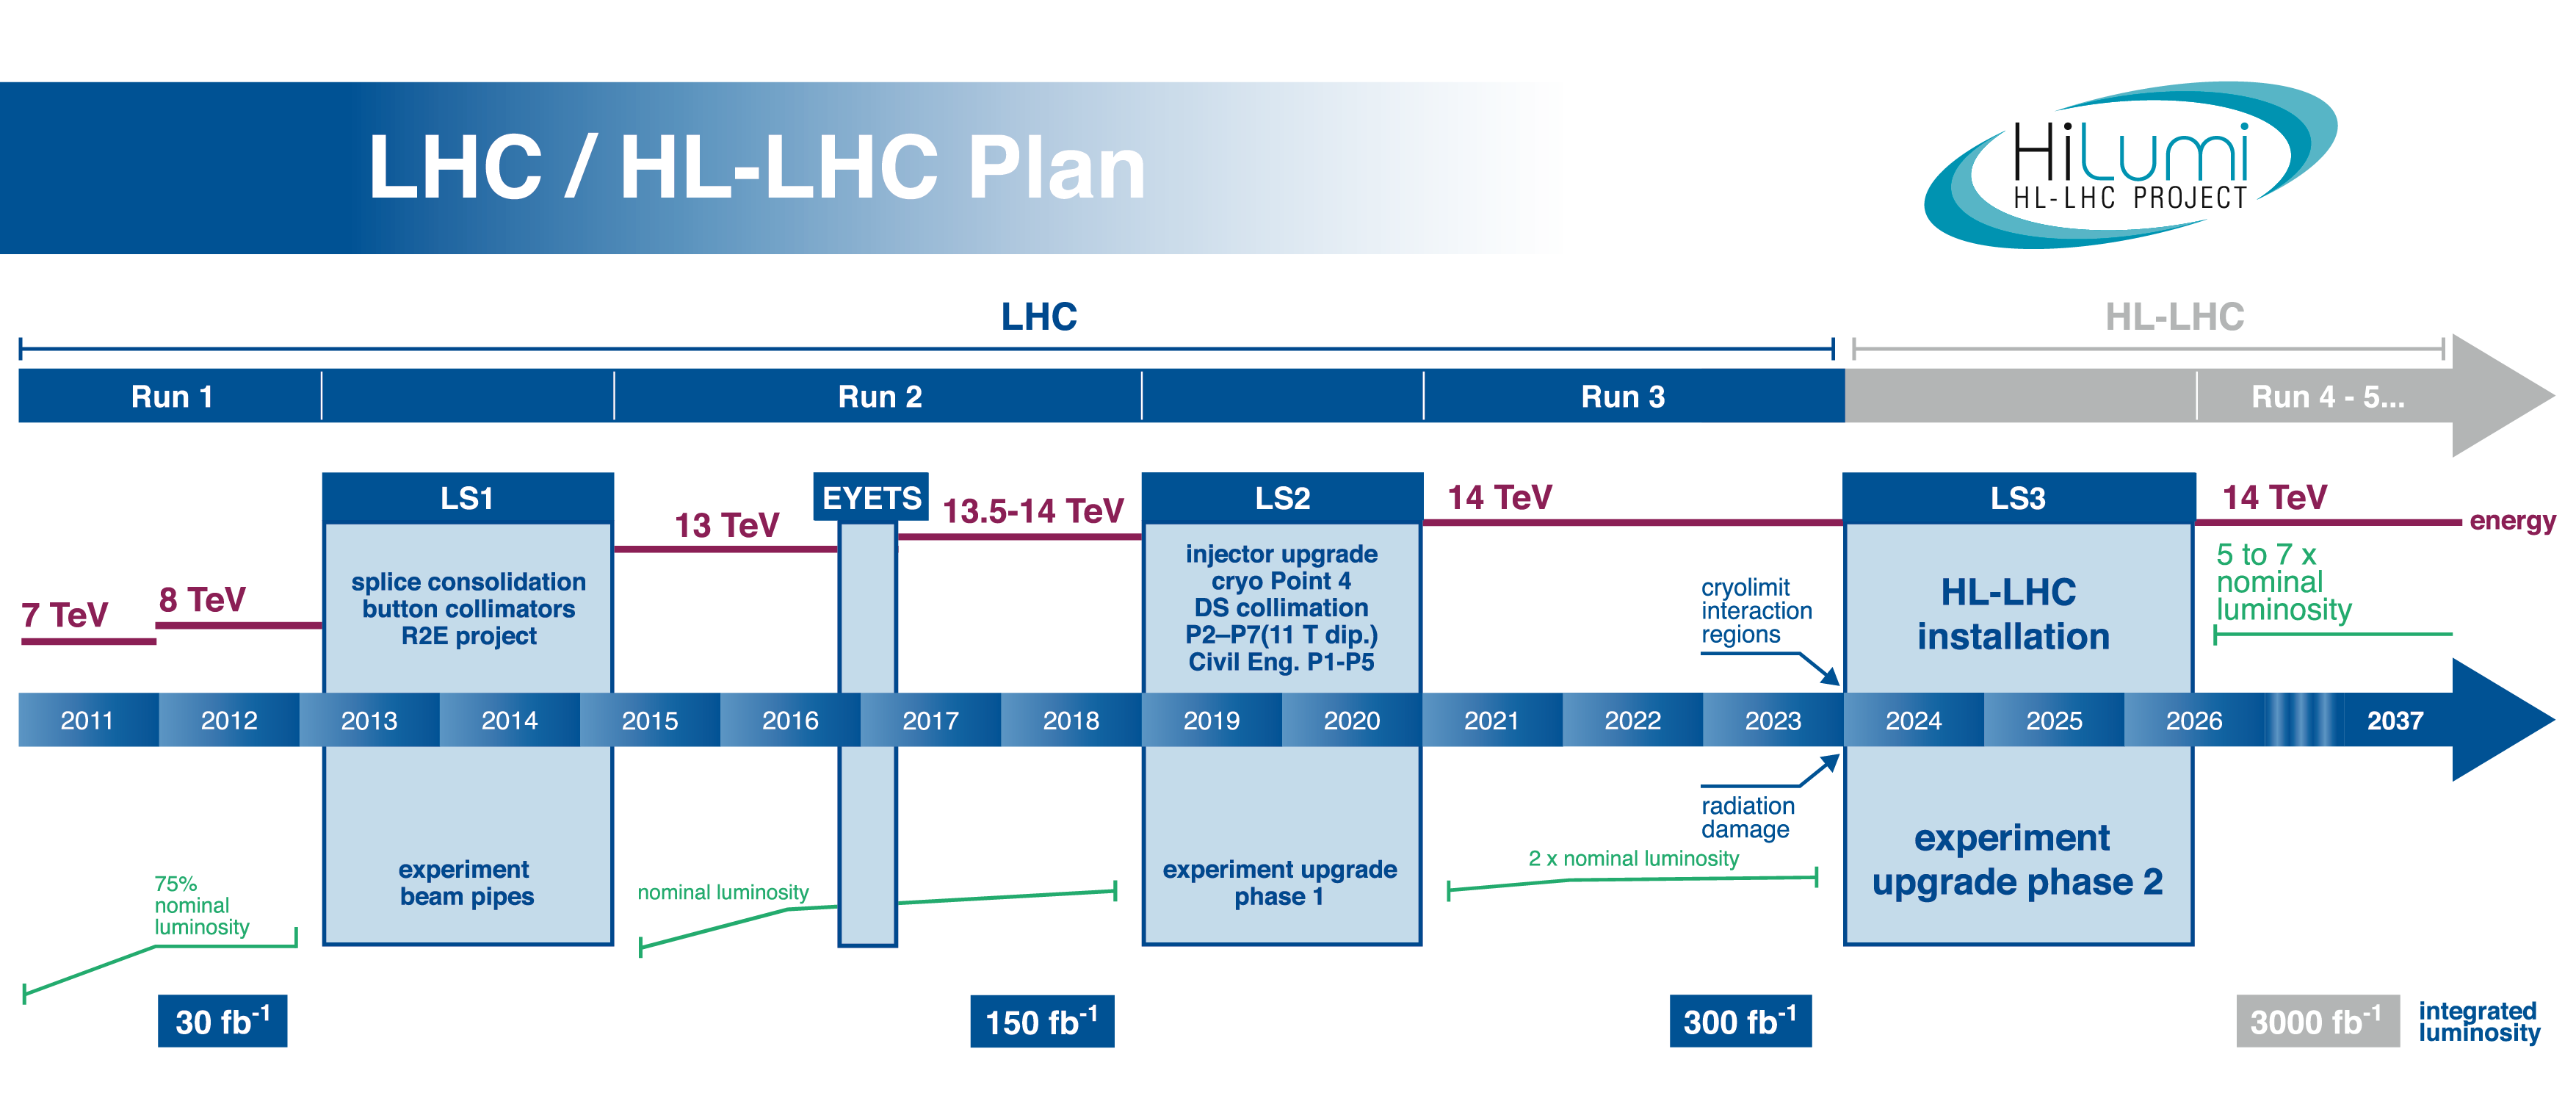
\includegraphics[width=1.\linewidth]{2_ExperimentalSetup/Figures/lhc_schedule}
	\caption{The HL-LHC timeline. Figure taken from \cite{Antonella:1975962}.}
	\label{fig:lhcschedule}
\end{figure}


Inside the LHC ring~\cite{Bruning:782076}, the protons are accelerated by the means of radio frequency cavities, while 1232 dipole magnets of approximately 15~\m\ long, each weighing 35~\tonne\, ensure the deflection of the beams.  The two proton beams circulate in opposite direction in separate pipes inside of the magnet. Through the use of a strong electric current in the coils of the magnet, magnetic fields are generated and cause the protons to bend in the required orbits. In order for the coil to become superconducting and able to produce a strong magnetic field of 8.3~\tesla, the magnet structure is surrounded by a vessel. This vessel is filled with liquid Helium making it possible to cool down the magnet to 1.9~\kelvin. In order to get more focussed and stabilised proton beams, additional higher-order multipole and corrector magnets are placed along the LHC beam line.

  

The LHC is home to seven experiments, each located at an interaction point: 
\begin{itemize}
	\item A Toroidal LHC ApparatuS (ATLAS)~\cite{Aad:2008zzm} and the Compact Muon Solenoid (CMS)~\cite{Chatrchyan:2008aa} experiments are the two general purpose detectors at the LHC. They both have a hermetic, cylindrical structure and were designed to search for new physics phenomena along with precision measurements of the Standard Model. The existence of two distinct experiments allows cross-confirmation of any discovery. 
	\item A Large Ion Collider Experiment (ALICE)~\cite{Aamodt:2008zz} and the LHC Beauty (LHCb)~\cite{Alves:2008zz} experiments are focusing on specific phenomena. ALICE studies strongly interacting matter at extreme energy densities where a quark-gluon plasma forms in heavy ion collisions (Pb-Pb or p-Pb). LHCb searches for differences between matter and antimatter with the focus on \Pbottom\ physics.
	\item The forward LHC (LHCf)~\cite{Bongi:2010zz} and the TOTal cross section, Elastic scattering and diffraction dissociation Measurement (TOTEM)~\cite{Anelli:2008zza} experiments are two smaller experiments that focus on head-on collisions. LHCf consists of two parts placed before and after ATLAS and studies particles created at very small angles. TOTEM is placed in the same cavern as CMS and measures the total proton-proton cross section and studies elastic and diffractive scattering.  
		\item The Monopoles and Exotics Detector At the LHC (MoEDAL)~\cite{Acharya:2014nyr} experiment is situated near LHCb and tries to find magnetic monopoles. 
\end{itemize}



 For the enhancement of the exploration of rare events and thus enhancing the number of collisions, high beam energies as well as high beam intensities are required. The luminosity~\cite{Gillies:1997001} is a measurement of the number of collisions that can be produced in a detector per square meter and per second and is the key role player in this enhancement. The LHC collisions create a number of events per second given by
\begin{equation}\label{eq:NbEv}
\centering
N_{\mathrm{event}} = L \sigma_{\mathrm{event}}, 
\end{equation}
where $\sigma_{\mathrm{event}}$ is the cross section of the process of interest and $L$ the machine  instantaneous luminosity. This luminosity depends only on the beam parameters and is for a Gaussian beam expressed as 
\begin{equation}\label{eq:Lumi}
	L = \frac{1}{4\pi}\textcolor{blue}{N_{\mathrm{b}} n_{\mathrm{b}} f_{rev}}\textcolor{red}{\frac{N_{\mathrm{b}}}{\epsilon_n }}\textcolor{darkgreen}{\left(1+\left(\frac{\theta_c \sigma_z}{2\sigma^*} \right)^2\right)^{\frac{-1}{2}}} \frac{\gamma_{\mathrm{r}}}{ \beta^*}.
\end{equation}
The number of particles per bunch is expressed by $N_{\mathrm{b}}$, while $n_{\mathrm{b}}$ is the number of bunches per beam, $f_{\mathrm{rev}}$ the revolution frequency, $\gamma_{\mathrm{r}}$ the relativistic gamma factor, $\epsilon_n$ the normalized transverse beam emittance - a quality for the confinement of the beam  , $\beta^*$ the beta function at the collision point - a measurement for the width of the beam, $\theta_c$ the angle between two beams at the interaction point, $\sigma_{\mathrm{z}}$ the mean length of one bunch, and $\sigma^*$ the mean height of one bunch. In \eq{eq:Lumi}, the blue part represents the stream of particles, the red part  the brilliance, and the green part  the geometric reduction factor due to the crossing angle at the interaction point.

The peak design luminosity for the LHC is $10^{34}\:\centi\m^{-2}\s^{-1}$, which leads to about 1 billion proton interactions per second. In 2016, the LHC was around 10\% above this design luminosity~\cite{Harriet:2212301}. The luminosity is not a constant in time since it diminishes due to collisions between the beams, and the interaction of the protons and the particle gas that is trapped in the centre of the vacuum tubes due to the magnetic field. The diffusion of the beam degrades the emittance and therefore also the luminosity. For this reason, the mean lifetime of a beam inside the LHC is around 15 \hour. The integrated luminosity - the luminosity provided in a certain time range - recorded by CMS and ATLAS over the year 2016 is given in \fig{fig:IntLumi}. In Run 2, the peak luminosity is 13-17$ \times 10^{33}\; \centi\m^{-2}\s^{-1}$ compared to 7.7$ \times 10^{33}\; \centi\m^{-2}\s^{-1}$ in Run 1. The recorded luminosity is validated for physics analysis keeping 35.9 \fbinv\ during 2016 data taking. 
% https://science.energy.gov/~/media/hep/hepap/pdf/201512/CMSRestart_Rakness_HEPAP_20151210.pdf
 \begin{figure}[htbp]
 	\centering
%	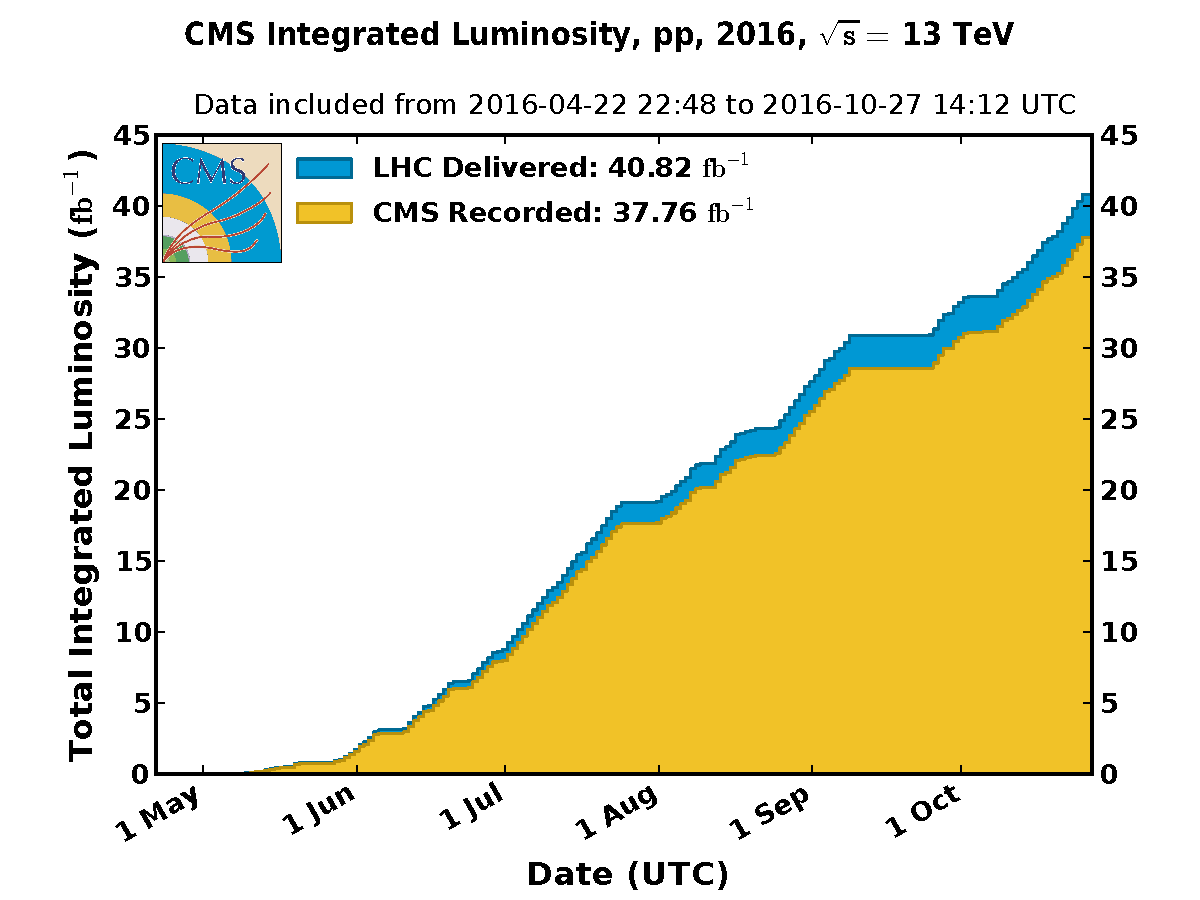
\includegraphics[width=0.7\textwidth]{2_ExperimentalSetup/Figures/int_lumi_per_day_cumulative_pp_2016.pdf}
	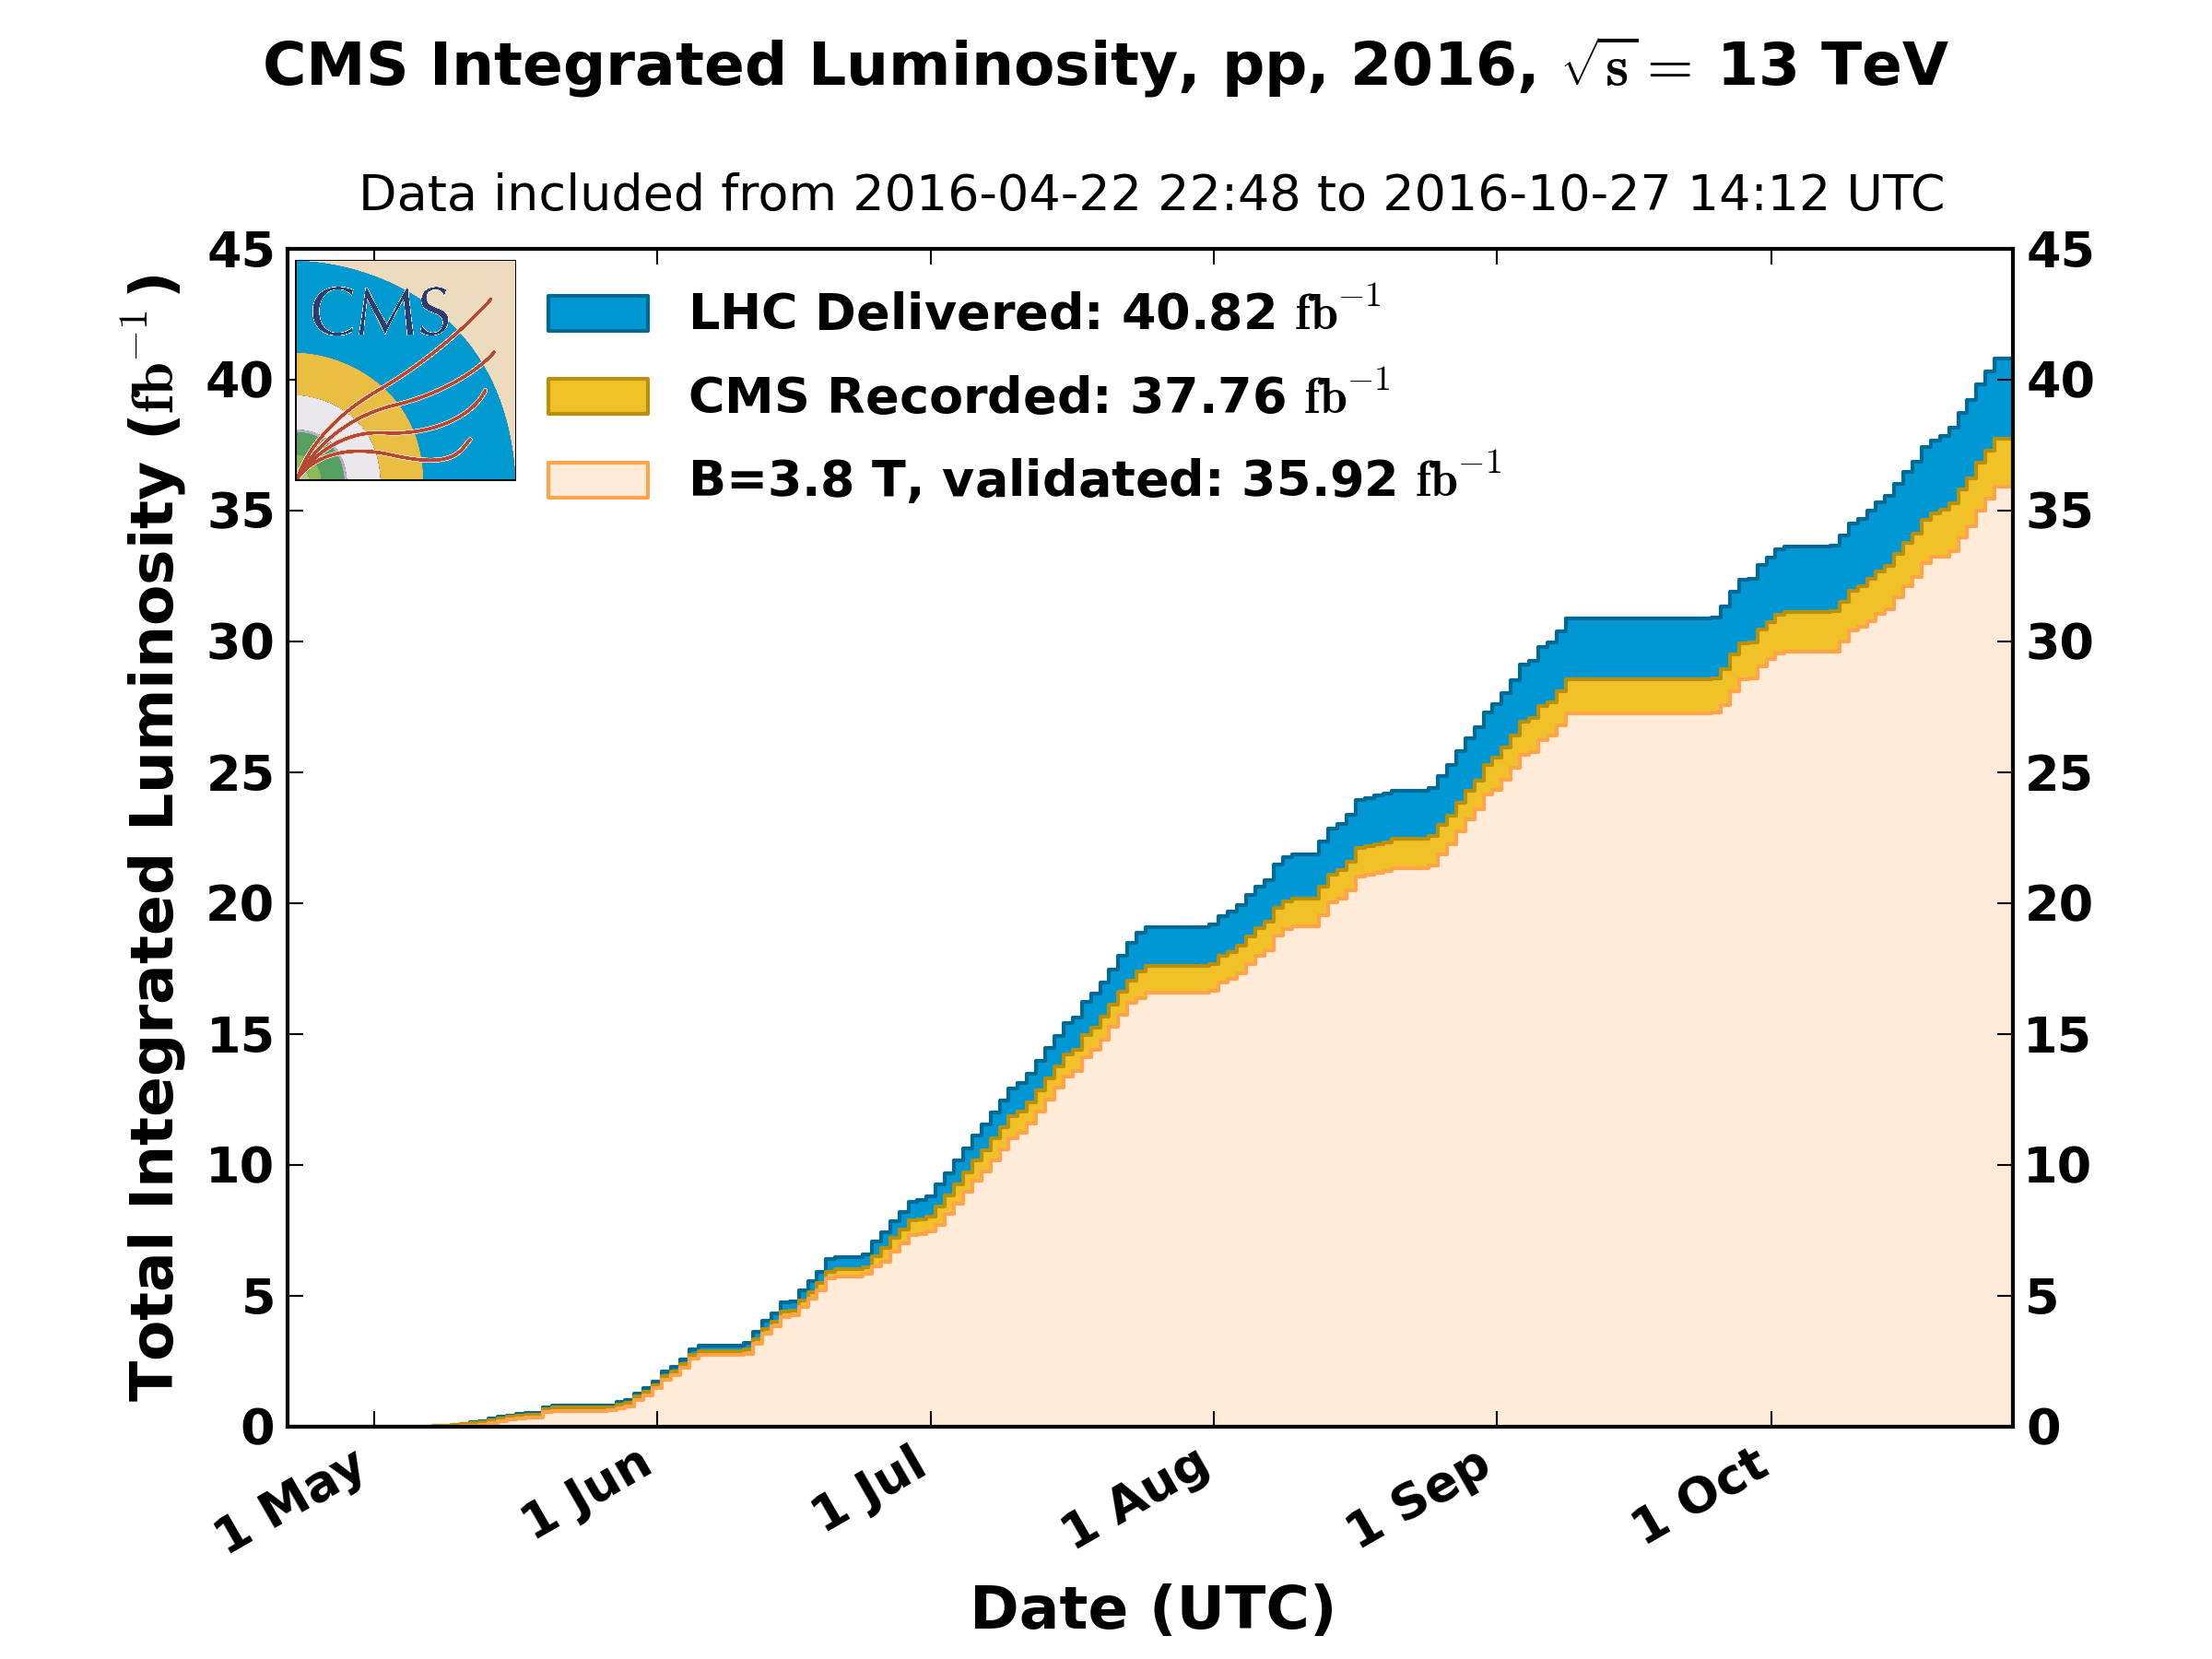
\includegraphics[width=0.7\textwidth]{2_ExperimentalSetup/Figures/int_lumi_per_day_cumulative_pp_2016_Golden_23Sep-PromEraH_Morion}
	\caption{Cumulative off-line luminosity measured versus day delivered by the LHC  (blue), and recorded by CMS (orange), and certified as good physics analysis during stable beams (light orange) during stable beams and for proton collisions at 13 TeV centre-of-mass energy in 2016.~\cite{LumiWiki}. }
	\label{fig:IntLumi}
%	(from https://twiki.cern.ch/twiki/bin/view/CMSPublic/LumiPublicResults#Online_Luminosity_AN2 )
%  https://twiki.cern.ch/twiki/bin/view/CMSPublic/DataQuality#2016_Proton_Proton_Collisions
\end{figure}
 
Multiple proton-proton interactions can occur during one  bunch crossing, referred to as \pu. On average, the number of \pu\ events is proportional to the luminosity times the total inelastic proton-proton cross section. In 2016,  an average of about 27 of \pu\ interactions has been observed in 13 \TeV\ proton collisions at the interaction point of CMS. For 2012, this number was about 21 \pu\ interactions for 8 \TeV\ collisions.



%CMS collaboration http://cds.cern.ch/record/2195940?ln=en map

\begin{comment}
% CMS Luminosity Measurement for the 2016 Data Taking Period`(CADI entry LUM-17-001)
% http://cms.cern.ch/iCMS/analysisadmin/cadi?ancode=LUM-17-001

CERN ACC 2017 0007 --> beam energy uncertainty

\end{comment}
\section{The Compact Muon Solenoid}
At one of the collision points of the LHC, the CMS detector\cite{CMS, Bayatian:2006zz,Bayatian:922757} is placed (see \fig{fig:CMS}). Weighing 14 000 \si{ \tonne}, This cylindrical detector is about 28.7 \si{ \meter} long and 15 \si{ \meter} in diameter, weighing around 14 000 \si{ \tonne}. It has an onion like structure of several specialised detectors and contains a superconducting solenoid with a magnetic field of 3.8 \si{ \Tesla}. The CMS detector is designed in a way that it can address the needs of physics coming from the LHC. Living in a hadronic environment, multi-jet processes produced by the strong interaction are a main source of background for rare physics processes. Therefore, good identification, momentum resolution, and charge determination of muon, electrons and photons is one of the main goals of the CMS detector. Further it provides a good charged particle momentum resolution and reconstruction efficiency in the inner tracker such that for example jets coming from b quarks or tau particles can be identified. Also the electromagnetic resolution for an efficient photon and lepton isolation as well as a good hadronic calorimeter for the missing transverse energy were kept into account while designing CMS. 

The LHC provides many collisions in a short amount of time. In order to discriminate between consecutive collisions - known as out of time pile up events - , CMS has to complete the full data acquisition for one collision event before the next one happen (around 25 \si{ \nano \second} in Run II and around 50 \si{ \nano \second} in Run I \cite{OLuanaigh:2051986}). Furthermore, since the photons are in packets, around 21 in Run I and 40 in Run II  inelastic collisions happen every beam crossing . This creates a great amount of background processes in the detector called in time pile up events. Due to this difficult conditions, the detector has a great granularity which on its turn creates a need for huge number of synchronized electronic channels. Furthermore, due to to high flux of particles in the regions close to the beam, the electronics has to be able to endure high radiation.


\begin{comment}
     \begin{figure}[ht]
	\centering
	\begin{minipage}[b]{0.4\textwidth}
		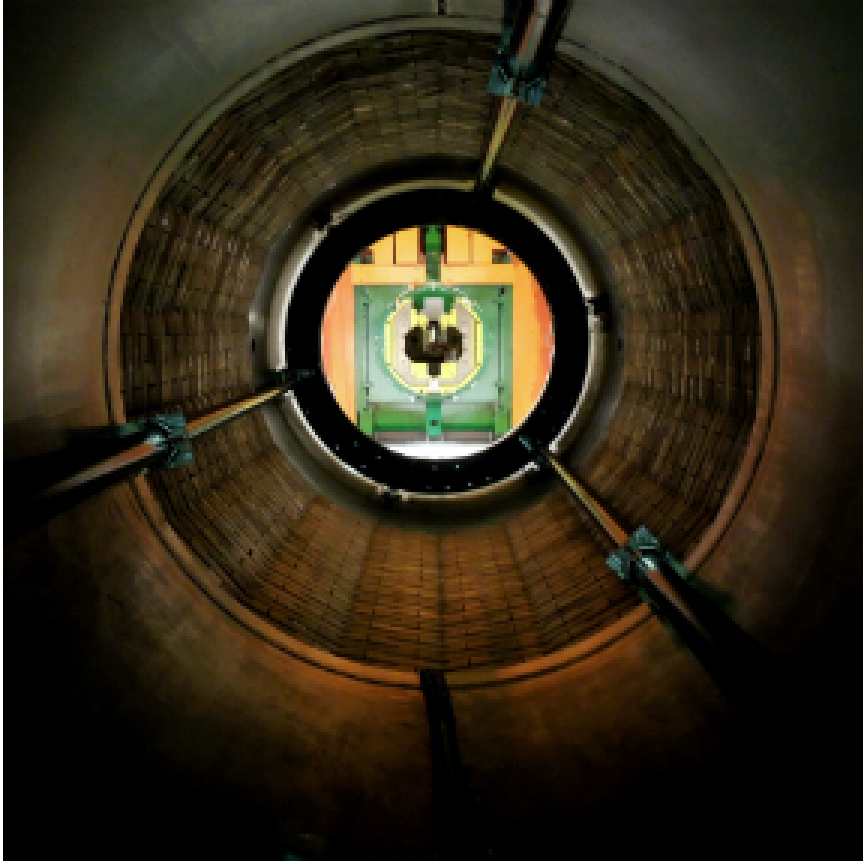
\includegraphics[width=\textwidth]{2_ExperimentalSetup/Figures/Beampipe}
		\caption{The LHC beampipe shown from inside CMS.(FIXME: use better resolution)}
	\end{minipage}
	\hfill
	\begin{minipage}[b]{0.4\textwidth}
		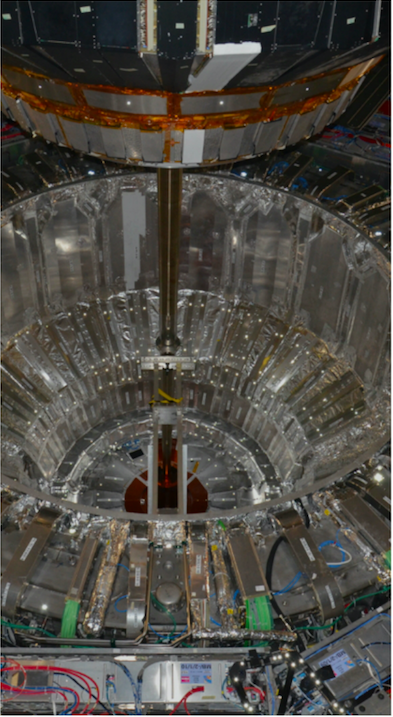
\includegraphics[width=\textwidth]{2_ExperimentalSetup/Figures/beampipe2}
		\caption{Beampipe going inside CMS. Picture taken from below (FIXME: use better resolution)}
	\end{minipage}
	\label{fig:IntLumi}
	%	(from https://twiki.cern.ch/twiki/bin/view/CMSPublic/LumiPublicResults#Online_Luminosity_AN2 )
\end{figure}
\end{comment}

\begin{figure}[ht]
	\centering
	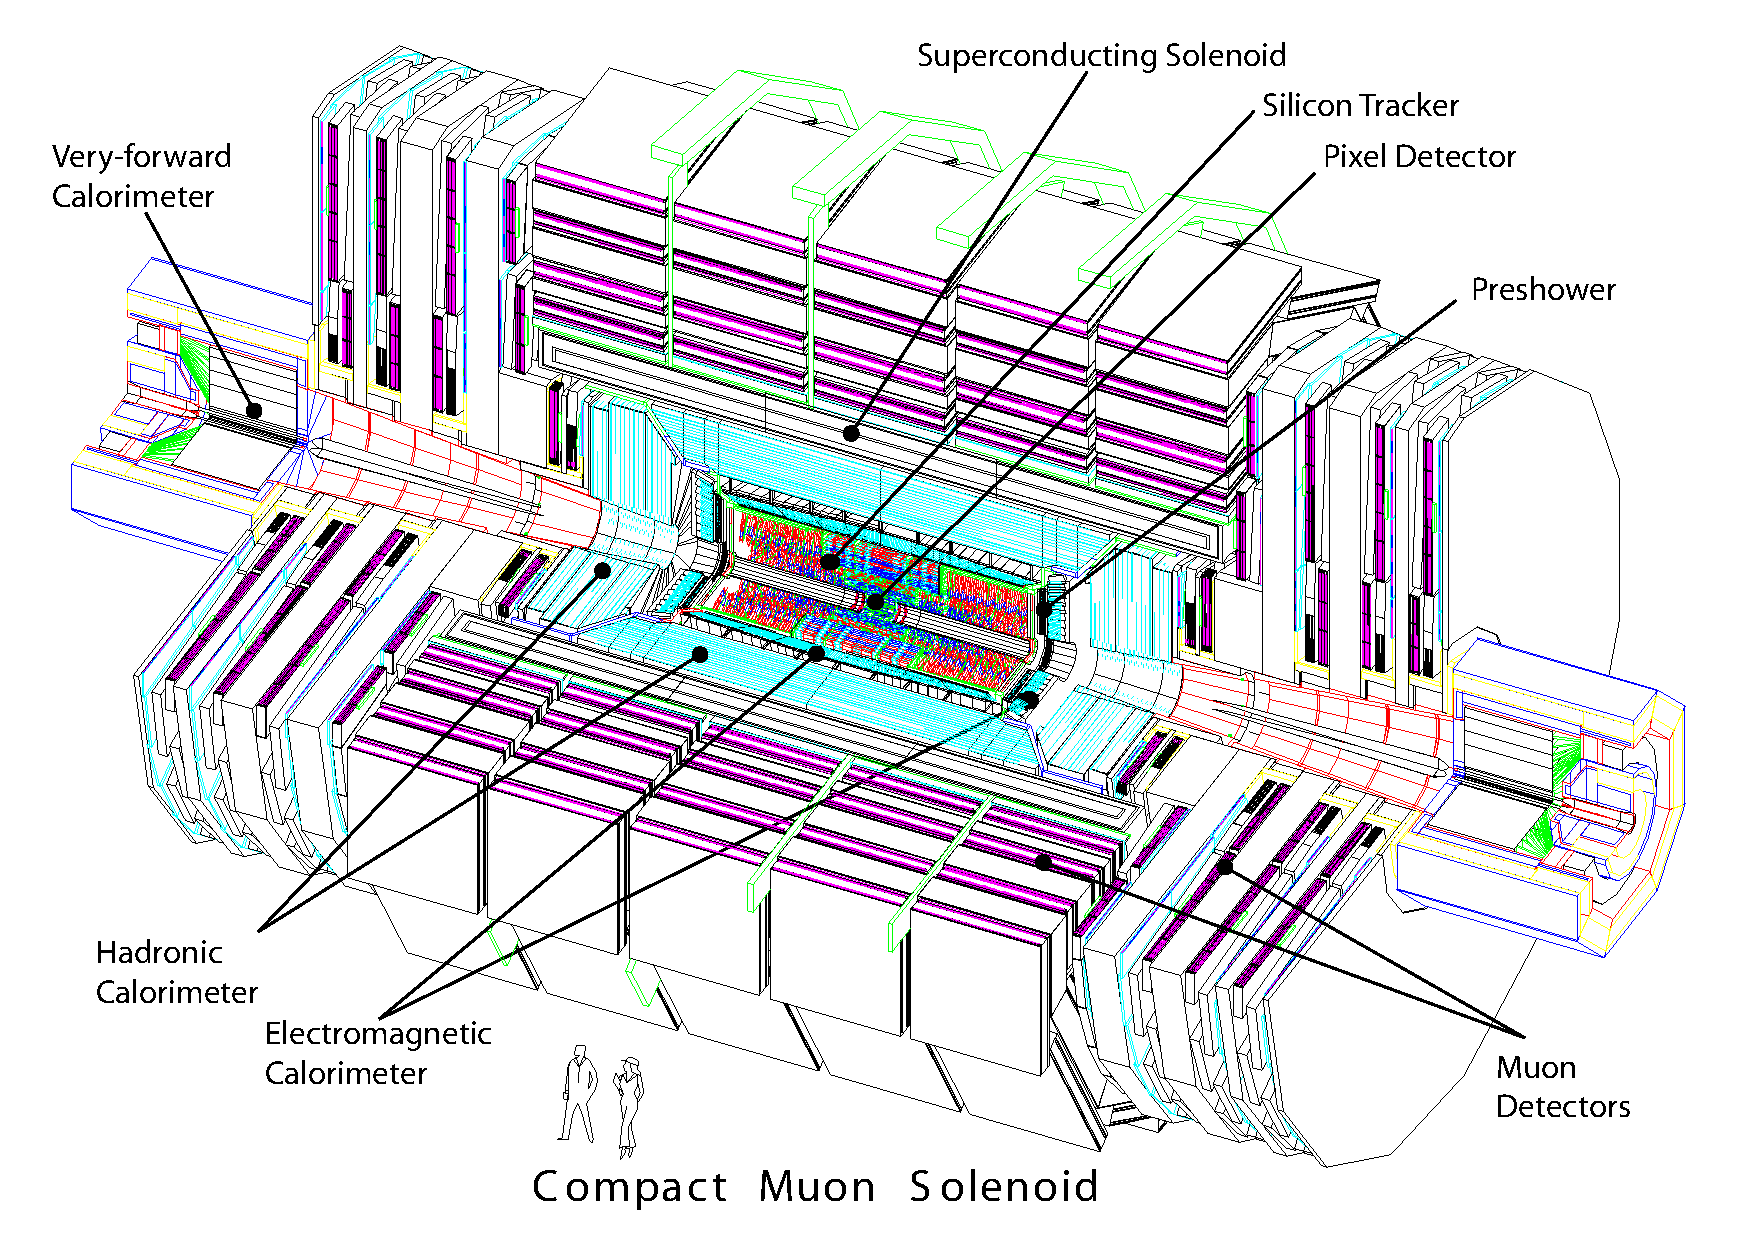
\includegraphics[width=\textwidth]{2_ExperimentalSetup/Figures/cms_complete_labelled}
	\caption{Mechanical layout of the CMS detector\cite{CMSdraw}.}
	\label{fig:CMS}
\end{figure}

Before the start of taking collision data for 13 \si{ \TeV} operations on 3 June, CMS had a long shutdown (LS1)\cite{Pralavorio:2024977}. During this shut down several upgrades were performed. The innermost part of detection material in CMS (pixel) is currently made of three concentric cylindrical layers. At the end of 2016 it is upgraded by adding a fourth layer, enhancing the particle tracking capabilities of CMS. In order to be able to incorporate this new layer, the section of the beryllium beam pipe within CMS was replaced by a narrower one during LS1. For this, the pixel was removed and reinserted into CMS.  In order to avoid long damage caused by the intense particle flux at the heart of CMS, the tracker is been made ready to operate at much lower temperature than before. During Run I, a small problem was detected in the electromagnetic calorimeter preshower system. For this, the preshower discs were removed, repaired and reinstalled successfully inside CMS in 2014. To help the discrimination between interesting low momentum muons coming from collisions and muons caused by backgrounds, a fourth triggering and measurement station for muons was added in each of the end caps.  CMS measures the collision rate within the detector and monitors beam related backgrounds. For this, several new detectors were installed into CMS during LS1. 


\newpage
\subsection{CMS coordinate system}
The coordinate system used by CMS can be found in \fig{fig:CMScoord}. The origin of the right handed orthogonal coordinate system is chosen to be the point of collisions. The x-axis points towards the centre of the LHC ring such that the y-axis points towards the sky, and the z-axis lies tangent to the beam axis. Since the experiment has a cylindrical shape, customary coordinates are used to describe the momentum \impuls: the distance $\rho$, the azimuthal angle $\phi \in \left[-\pi,\pi\right]$ - the angle between the x-axis and the projection in the transverse plane of \impuls (\trimpuls) - , the pseudo-rapidity \psrap - expressed by the polar angle $\theta$ between the direction of \impuls and the beam - : 
\begin{equation}
\eta = - \ln \left(\tan \left(\frac{\theta}{2}\right)\right).
\end{equation}
For the energies considered at the LHC, where $E >> m$, the pseudo-rapidity is a good approximation of the rapidity $y$
\begin{equation}
y = \frac{1}{2} \ln \left(\frac{E + p_z}{E - p_z}\right), 
\end{equation}
where the difference of rapidities of two particles is invariant under a Lorentz boost in the z-direction.
 \begin{figure}[ht]
	\centering
	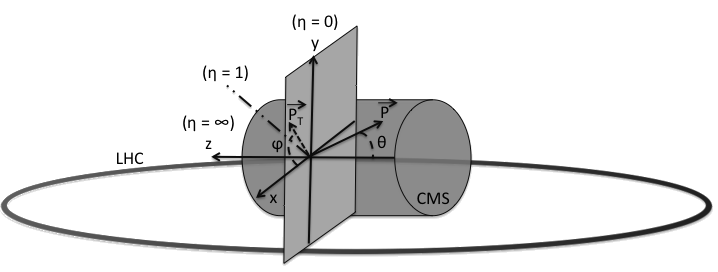
\includegraphics[width=0.75\textwidth]{2_ExperimentalSetup/Figures/imageedit_1_9146672677}
	\caption{Representation of the coordinate system used by CMS. The point of origin is put at the collision point. The x-axis points towards the centre of the LHC ring such that the z-axis lies tangent to the beam axis. }
	\label{fig:CMScoord}
\end{figure}

\subsection{Towards the heart of CMS}
The CMS detector consists of two parts; a central barrel around the beam pipe (\abspsrap $<1.4$) and two plugs to ensure the hermeticity of the detector. In \fig{fig:CMS} and \fig{CMSview} the onion like structure of the CMS detector is visible. The choice of a solenoid of 12.9 \si{ \meter}  long and 5.9 \si{ \meter}
diameter gives the advantage of bending the particle trajectories in the transverse plane. The hadronic calorimeter,  the electromagnetic calorimeter and the tracker are within the solenoid, while the muon chambers are placed outside the solenoid.



\begin{figure}[ht!]
	\centering
	\includegraphics[width=0.45\textwidth]{2_ExperimentalSetup/Figures/cmsview1}
	\includegraphics[width=0.45\textwidth]{2_ExperimentalSetup/Figures/cmsview}
 \caption{Schematic view of the CMS detector in the Run I configuration. (LEFT) Longitudinal view of one quarter of the detector. (RIGHT)  Transversal view of one quarter of the detector. The muon system barrel elements are denoted as MBZ/N/S, where z$=-2...+2$ is the barrel wheel number, n$=1...4$ the station number and S$=1...12$ the sector number. Similary, the steel return yokes are denoted as YBZ/N/S. The solenoid is denoted as CB0, while the hadronic calorimeter is denoted as HE (end cap)/ HB (barrel)/HF(forward) and the electromagnet calorimeter as EE(end cap)/EB (barrel). The green part represents the tracking system\cite{Chatrchyan:1223944}}.
	\label{fig:CMSview}
\end{figure}

\subsubsection{Muon system}
The outermost part of CMS consists of the muon system. The magnet return yoke is interleaved with gaseous detector chambers for muon identifictaion nd momentum measurement. The barrel contains muon stations arranged in five separate iron wheels, while in the end cap four muon stations are mounted onto three independent iron discs in on each side. Each barrel wheel as 12 sectors in the azimuthal angle. 

The muon system is divided into three parts\cite{Chatrchyan:1223944}, shown in \fig{fig:muonsys}. The muon rate and neutron induced backgrounds are small and the magnetic field is very low for the barrel and CMS can use drift tube (DT) chambers. For the end caps however, the muon and background flux is much higher and there is a need to use cathode strip chambers (CSC) which are able to provide a faster response, higher granularity and a better resistance against radiation. In order to form a redundant trigger system, resistive plate chambers (RPC) are added. This makes a total of 250 DT chambers, 540 CSC and 610 RPC. In \fig{fig:CMSview} the arrangement is shown.


\begin{figure}[ht!]
	\centering
	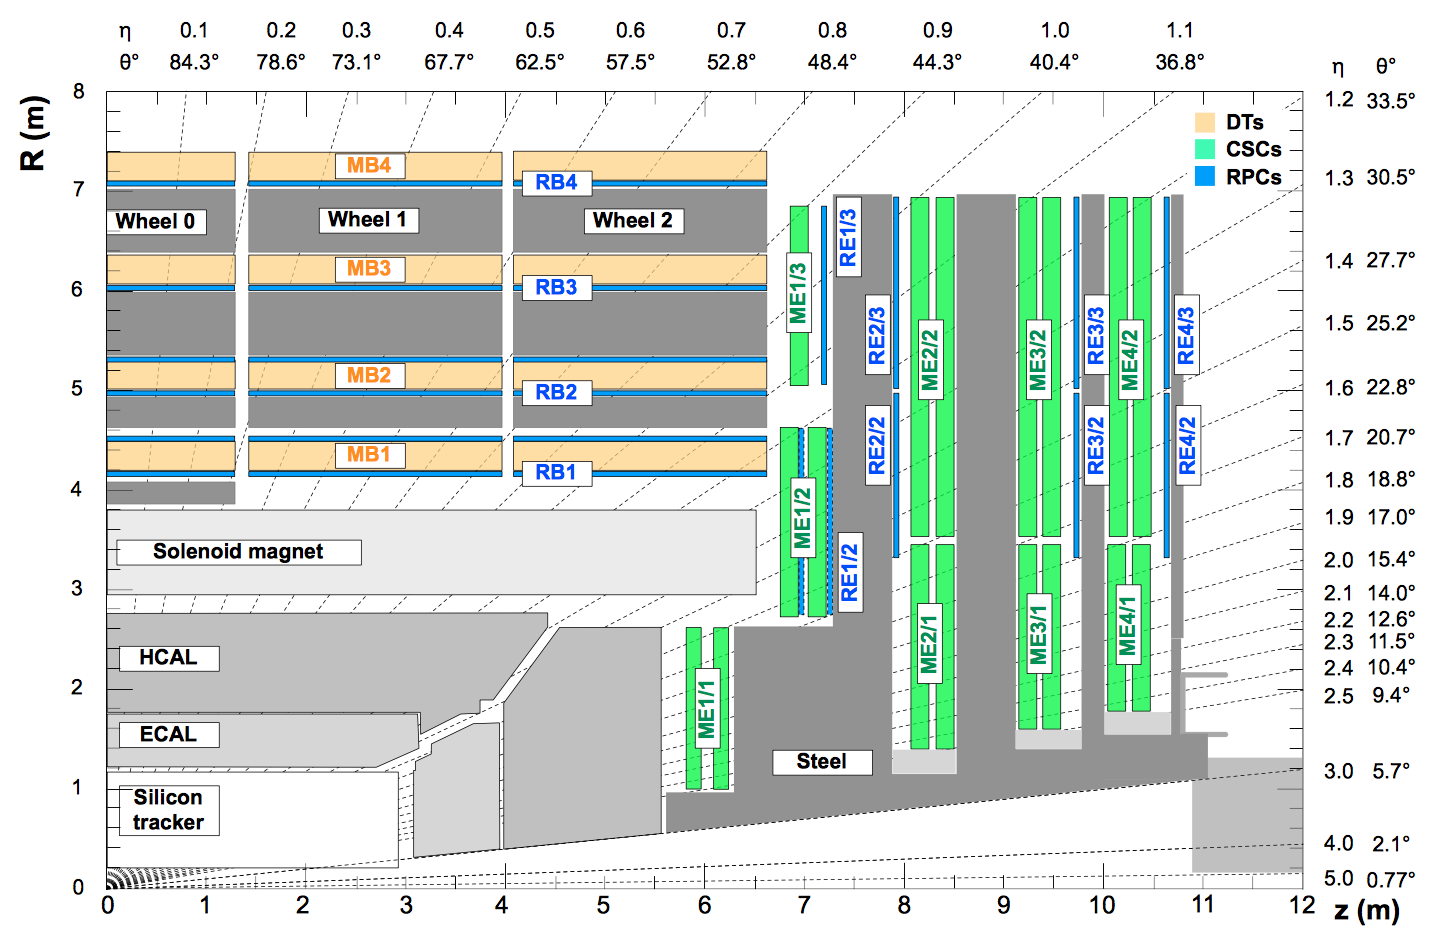
\includegraphics[width=0.6\textwidth]{2_ExperimentalSetup/Figures/muonsys}
	\caption{Schematic view of one quarter of the CMS muon system in the Run I configuration. \cite{Chatrchyan:1223944}}.
	\label{fig:muonsys}
\end{figure}


Providing a measurement for \abspsrap $<1.2$. The DT chambers in the barrel are on average 2 $\times$ 2.5 \si{ \meter} in size and consist of 12 layers of DT cells - 4 \si{ \centi \meter} wide gas tubes with positively charged stretched wire inside - arranged in three groups of four. The $r\phi$ coordinate is provided by the two outside groups, while the middle group measures the $z$ coordinate. For each $\phi$ sector, the DT chamber is mixed with the flux return yoke. For the outer muon station, the DT chamber contains only 8 layers of DT cells, providing a muon position in th $r\phi$ plane.
There are four CSC stations in each end cap, providing muon measurements for $0.9<$ \abspsrap $<2.4$ (Run I configuration). These CSC are multi-wired proportional chambers that consist of 6 anode wire planes crossed by 7 copper strips cathode panels in a gas volume. The $r$ coordinate is provided by the copper strips, while $\phi$ coordinate comes from the anode wires, giving a two dimensional position measurement. 
There are six layers of RPC in the barrel muon system and one layer into each of the first three stations of the end cap. They are made from two high resistive plastic plates with an applied voltage and separated by a gas volume. Read out strips mounted on top of on of the plastic plates detects the signal generated by a muon passing through the gas volume. The RPC provides a fast response with a time resolution of 1 \si{ \nano \second} and cover a range of \abspsrap $<1.8$ (Run I configuration). 


During the long shutdown, the  muon system underwent major upgrades~\cite{Guiducci:1966038,Battilana:2239185}. In the fourth station of each end cap, the outermost rings of CSC and RPC chambers were completed, providing an angular region of $1.2<$ \abspsrap $<1.8$ for Run II, increasing the system redundancy, and allowing tighter cuts on the trigger quality. In order te reduce the environmental noise, outer yoke discs have been placed on both sides for the end caps. 
At the innermost rings of the first station, the CSC has been upgraded by refurbishing the readout electronics to make use of the full detector granularity instead of groups of three (Run I). 


The muon system provides triggering on muons, identifying muons and improves the momentum measurement and charge determination of high $p_T$ muons. On top of the muon system, the muon energy is deposited in the electromagnetic calorimeter, the hadronic calorimeter, and outer calorimeter. (FIXME not tracker?) The high magnetic field enable an efficient first level trigger and allows a good momentum resolution of $\Delta ^p / p \approx 1\%$ for a $p_T$ of 100 \si{ \GeV} and $\approx 10\%$ for a $p_T$ of 1 \si{ \TeV} (FIXME). There is an efficient muon measurement up to \abspsrap $<2.4$.
\subsubsection*{Muon reconstruction}
% see http://www.bo.infn.it/sminiato/sm16/03_Mercoledi/Mattina/01_Battilana.pdf
% see https://arxiv.org/pdf/1510.05424.pdf
% see https://twiki.cern.ch/twiki/bin/view/CMSPublic/MuonDPGPublic160729
 The muon reconstruction\cite{Chatrchyan:2012xi} has three subdivision: local reconstruction, regional reconstruction and global reconstruction. 
The local reconstruction is performed on individual detector elements such as strip and pixel hits in the inner tracking system, and muon hits and/or segments on the muon chambers. Independent tracks are reconstructed in the inner tracker - called tracker track -  and in the muon system, called standalone tracks.
Based on these tracks, two reconstructions are considered.
The outside-in approach is referred to as Global Muon reconstruction. 
 For each standalone track, a tracker track is found by comparing the parameters of the two tracks propagated onto a common surface. Combining the hits from the tracker track and the standalone track, gives a fit via the Kalman filter technique~\cite{FRUHWIRTH1987444,Billoir:1989mh} for a global muon track. 
 The second approach is an inside-out reconstruction, creating tracker muons. 
 All candidate tracker tracks are extrapolated to the muon system taking into account the magnetic field, the average expected energy losses, and multiple Coulomb scattering in the detector material. When at least one muon segment - DT or CSC hits -  matches the extrapolated track, the corresponding tracker track is indicated as a tracker muon. 
 
 For low transverse momenta ($p_T \lesssim$ 5 \si{ \GeV}), the tracker muon reconstruction is  more efficient than the global muon approach. This is due to the fact that tracker muons only require a single muon  segment in muon system, while the global muon approach requires typically segments in at least two muon stations. Therefore, the global muon approach typically improves the tracker reconstruction for $p_T\gtrsim$ 200 \si{ \GeV}.
 The tming 

\subsubsection{Solenoid}
	Making use of the knowledge of previous experiments of ALEPH and DELPHI at LEP and H1 at HERA, CMS choose for a large super conducting solenoid with a a length of 12.9 \si{ \meter} and a inner bore of 5.9 \si{ \meter}\cite{Bayatian:922757}. With 2 168 turns, a -current of 19.5 \si{ \kilo \ampere} and  a total energy of 2.7 \si{ \giga \joule}, a large bending power can be obtained for a modestly-sized solenoid. In order to ensure a good momentum resolution in the forward regions, a favourable length/radius was necessary.  In \fig{fig:CMSsolenoid}, a photo of the CMS solenoid is given. 

	The solenoid uses a high-purity aluminium stabilised conductor with indirect cooling from liquid helium, together wit fully epoxy impregnation. A four-layer winding is implemented that can withstand an outward pressure of 64 \si{ \atm}. The NbTi cable is co-extruded by pure aluminium that acts as a thermal stabilizer and has an aluminium alloy for mechanical reinforcement. The return of the magnetic field is done by fives wheels, noted by YB in \fig{fig:CMSview}.
	
	\begin{figure}[ht]
		\centering
		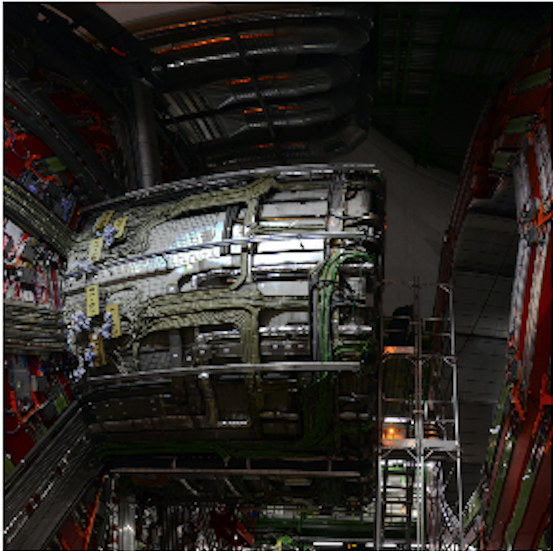
\includegraphics[width=0.45\textwidth]{2_ExperimentalSetup/Figures/solenoid}
		\caption{CMS solenoid during the long shutdown in 2013. }
		\label{fig:CMSsolenoid}
	\end{figure}	
	
\subsubsection{Hadronic calorimeter}
% http://cds.cern.ch/record/2235509?ln=en peformance
The hadronic calorimeter (HCAL) is dedicated to precisely measure the energy of charged and neutral hadrons via a succession of absorbers and scintillators. This makes it crucial for physics analyses with hadronic jets or missing transverse energy. The HCAL extends between 1.77 $<r<$ 2.95 \si{ \meter} where $r$ is the radius in the transverse plane with respect to the beam. Due to space limitations, the HCAL needs to be as small as possible and is made from materials with short interaction lengths - the length needed for absorbing 36.7\% of the hadrons. The quality of the energy measurements is dependant on the fraction of the hadronic shower that can be detected. Therefore, the HCAL barrel (HB) inside the solenoid is reinforced by an outer hadronic calorimeter between the solenoid and muon detectors (HO, see \fig{fig:HCAL}), using the solenoid as extra absorber. This increases the thickness to 12 interaction lengths. Furthermore, it should be as hermetic as possible and extend to large pseudo rapidity values. The HB and HO provide measurements for \abspsrap $<1.3$, while an end cap on each side (HE,$1.3<$ \abspsrap $<3$) and a forward calorimeter (HF, \abspsrap < 5.2) extend the pseudo rapidity range. 


\begin{figure}[ht]
	\centering
	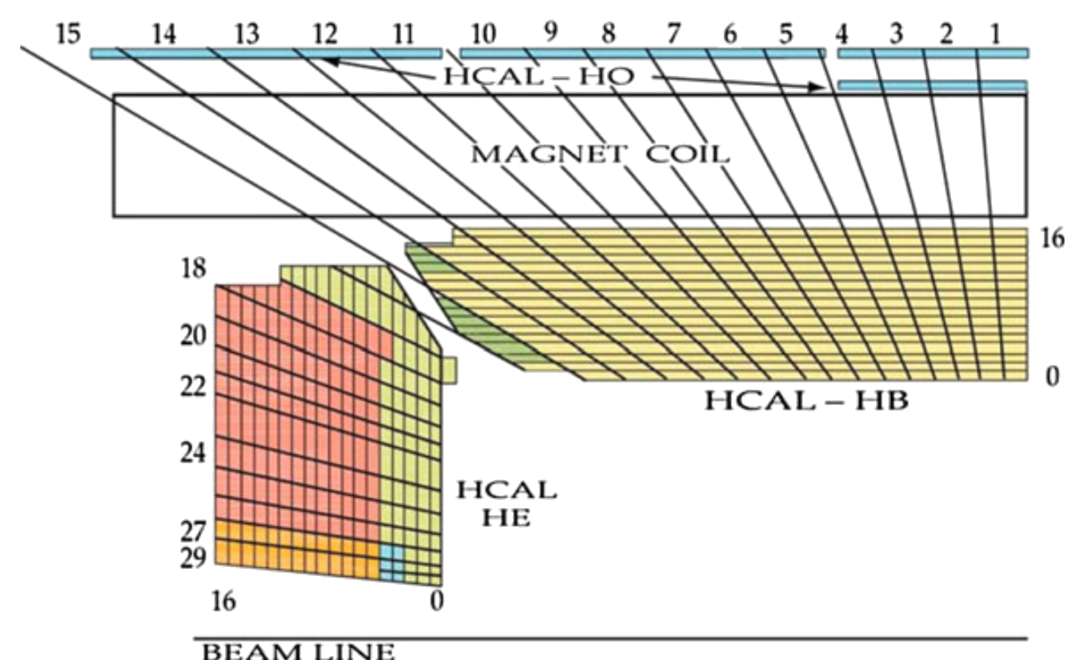
\includegraphics[width=0.5\textwidth]{2_ExperimentalSetup/Figures/imageedit_12_3242046754}
	\caption{Tower segmentation for one quarter of the HCAL displayed in the $rz$ plane\cite{Chatrchyan:2008aa}.}
	\label{fig:HCAL}
\end{figure}

The HB is made of 16 absorber plates where most of them are built from brass and others are made from stainless steal and is about five to ten intercation lengths thick. The HE is also composed of brass absorber plates and has a thickness corresponding to approximately ten interaction lengths. 
The HF experiences intense particle fluxes with an energy of 760 \si{ \GeV} deposited on average in a proton interaction at a center of mass of 14 \si{ \TeV}, compared to 100 \si{ \GeV} in the rest of the detector. Therefore, these are Cherenkov light detectors made of radiation hard quartz fibers.
The main causes of such large energy events is high energy muons, cosmic particles and charged particles from late showering hadrons. During  Run I, it became clear that the glass windows of the PMTs had to be replaced which was done during the long shut down \cite{Tiras:2016ghv}
	
\subsubsection{Electromagnetic calorimeter}
The electromagnetic calorimeter (ECAL) is designed to measure the energy of photons and electrons and covers \abspsrap $<3$. It is an hermetic, homogeneous detector and consists of 75 848 lead tungstate (PbW$O_4$) crystals. These crystals have a fast response time - 80\% of the light is emitted within 25 \si{ \nano \second} - and are radiation hard. The electromagnetic showers produced by passing electrons or photons ionize the crystal atoms which emit a blue-green scintillation light, that is collected by silicon avalanche photodiodes (APDs) in the barrel and vacuum phototriodes (VPTs) in the end caps. The crystals and the APD response is sensitive to temperature changes and require a stable temperature. 

\begin{figure}[ht]
	\centering
	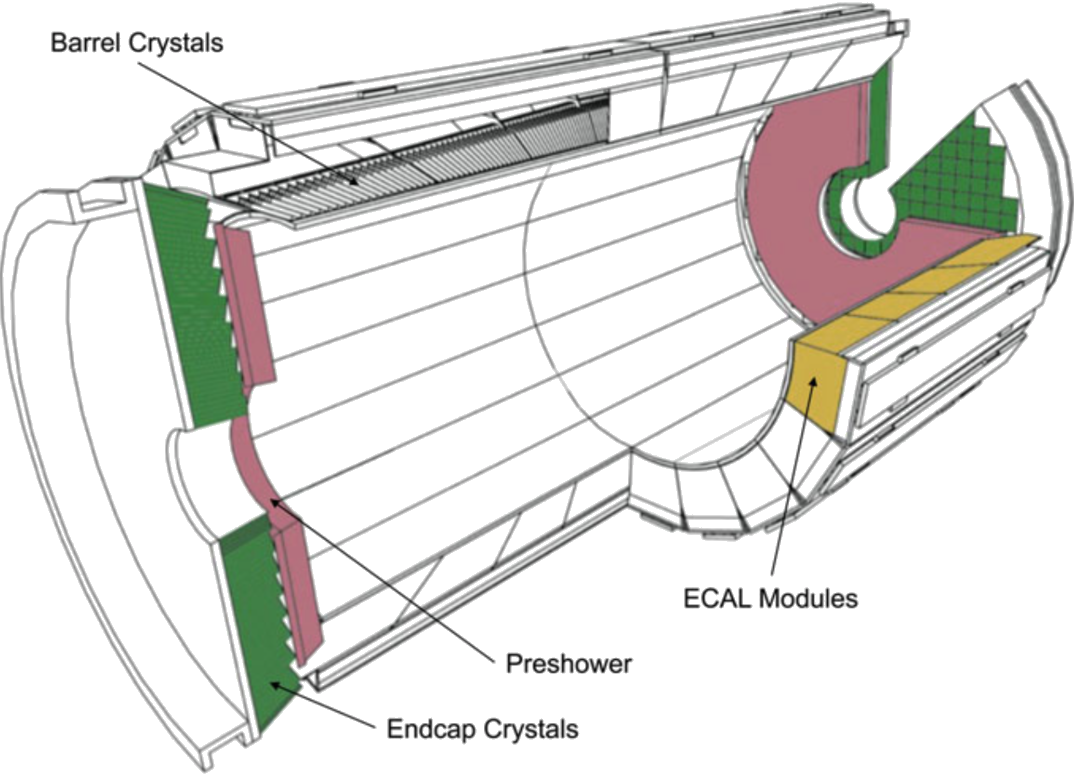
\includegraphics[width=0.5\textwidth]{2_ExperimentalSetup/Figures/imageedit_5_8264930617}
	\caption{Schematic cross section of the electromagnetic calorimeter\cite{Chatrchyan:2008aa}.}
	\label{fig:ECAL}
\end{figure}
There are three regions: a central barrel (EB), a endcap region (EE) and a preshower (ES) (\fig{fig:ECAL}). 
The EB has an inner radius of 129 \si{ \centi \meter} and corresponds to a pseudo rapidity of $0 < $ \abspsrap $<1.479$. At a distance of 314 \si{ \cent \meter} from the vertex and covering a pseudo rapidity of $1.479 < $ \abspsrap $<3.0$, are the EE. They consist of semi-circular aluminium plates from which structural units of $5\times5$ crystals (super crystals) are supported. The ES is placed in front of the crystal calorimeter over the end cap pseudo rapidity range with two planes of silicon strip detectors as active elements. 

The electromagnetic shower will typically involve more then one channel. More than 90\% of the energy of a 35 \si{ \GeV} electron or photon is contained in a $5\times 5$ matrix of crystals. Therefore, a clustering algorithm is performed in order to associate the energy deposits to the particles impinging the calorimeter.
The achieved precision\cite{1748-0221-12-01-C01069} for the barrel is 2.10$^{-3}$ \si{ \rad} in $\phi$ and 10$^{-3}$ in \psrap. For the end caps this is 5.10$^{-3}$ \si{ \rad} in $\phi$ and 2.10$^{-3}$ in \psrap. The energy is reconstructed by a super cluster algorithm, taking into account energy radiated via bremsstrahlung or conversion: 
\begin{equation}
E_{e/\gamma} = G F_{e/\gamma} \sum_{i \in cluster} S_i(t) VC_i A_i,
\end{equation}
where $G$ is the absolute energy scale in \si{ \GeV \per \ADC}, $F$ the energy containment corrections (depends on type of particle, its energy and pseudo rapidity, eg shower leakage and bremsstrahlung losses for electrons), $S(t)$ the relative channel variation with time, $C$ the relative channel response and $A$ the amplitude in \si{ \ADC} counts. The energy resolution is given by 
\begin{equation}
\frac{\sigma(E)}{E} = \frac{2.8\%}{\sqrt{E}}\oplus \frac{0.128}{E(GeV)} \oplus 0.3\%, 
\end{equation}
in the absence of a magnetic field, where the contributions come from the stochastic, noise and constant terms respectively. The dominating term is the constant term ($E_{shower} \approx 100 GeV$) and thus the performance is highly dependent on the quality of calibration and monitoring .

In Run I, the energy reconstruction happened  via a weighted sum of the digitized samples\cite{Chatrchyan:2013dga}. For Run II however, the reconstruction had to be made more resistant for out of time pile up and a multi-fit approach has been set in to place. In this approach, the pulse shape is modelled as a sum of one in-time pulse plus the out of time pulses \cite{1748-0221-12-01-C01069}. The energy resolution is less than 2\%  in the central barrel region and 2-5 \% elsewhere.
% https://indico.cern.ch/event/477407/contributions/2305075/attachments/1368970/2075215/hc16-edm.pdf
% see http://iopscience.iop.org/article/10.1088/1748-0221/12/01/C01069/pdf at vub
% http://www.bo.infn.it/sminiato/sm16/03_Mercoledi/Sera/08_Brianza.pdf
% https://indico.cern.ch/event/472938/contributions/1150724/attachments/1273518/1888397/ECALEnergyOverview_CALOR.pdf
%https://inspirehep.net/record/1344855/files/10.1088_1742-6596_587_1_012001.pdf
\begin{comment}
The relative energy resolution of the ECAL for electrons is between 1.4-3\% in EB and 3-4\% for EE. In Figure \ref{fig:ECALres}, the resolutions for low and high bremsstrahlung electrons are shown. 
\begin{figure}[ht]
	\centering
	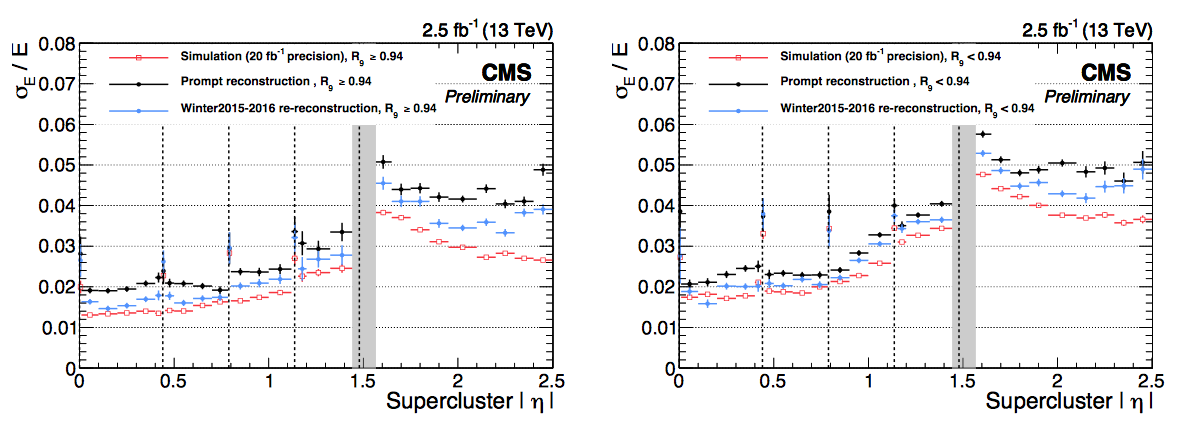
\includegraphics[width=\textwidth]{2_ExperimentalSetup/Figures/imageedit_7_5931623976}
	\caption{Relative energy resolution in bins of pseudo rapidity for the barrel and end caps using electrons from $Z \rightarrow ee$. Left: low bremsstrahlung electrons, Right: high bremsstrahlung electrons\cite{Sun:2233637}.}
	\label{fig:ECALres}
\end{figure}
\end{comment}

\subsubsection{Inner tracking system and operations}
%https://indico.cern.ch/event/632928/
%http://cds.cern.ch/search?ln=en&cc=CMS+Reports&sc=1&p=tracker&f=title&action_search=Search
% comparison with atlas https://cds.cern.ch/record/1563583/files/ATL-PHYS-PROC-2013-206.pdf
The tracking system (tracker)~\cite{Chatrchyan:1704291} is the detecting unit closest to the point of interaction. Responsible for the reconstruction of  trajectories from charged particles with \abspsrap $<2.5$, being bend by the magnetic field, it provides a measurement of the momentum. The tracker is also responsible for the determination of the interaction point or vertex. It should be able to provide high granularity as well as speed, and be able to endure high radiation. For this reason, the CMS collaboration choose silicon detector technology.

\begin{figure}[ht]
	\centering
%	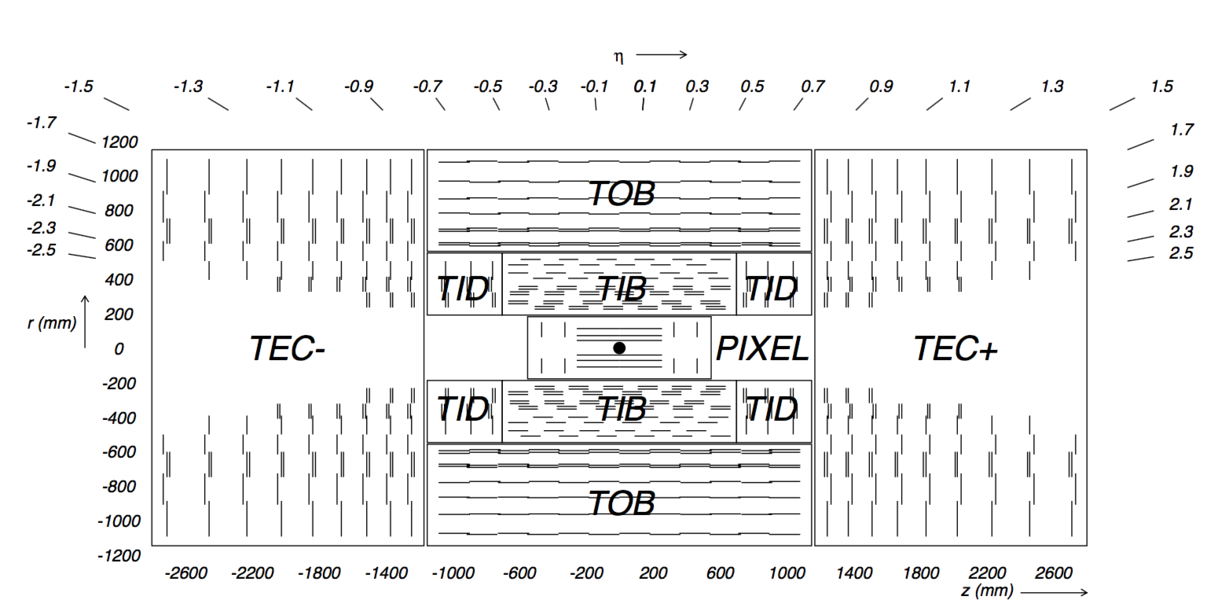
\includegraphics[width=\textwidth]{2_ExperimentalSetup/Figures/imageedit_3_5170744545}
	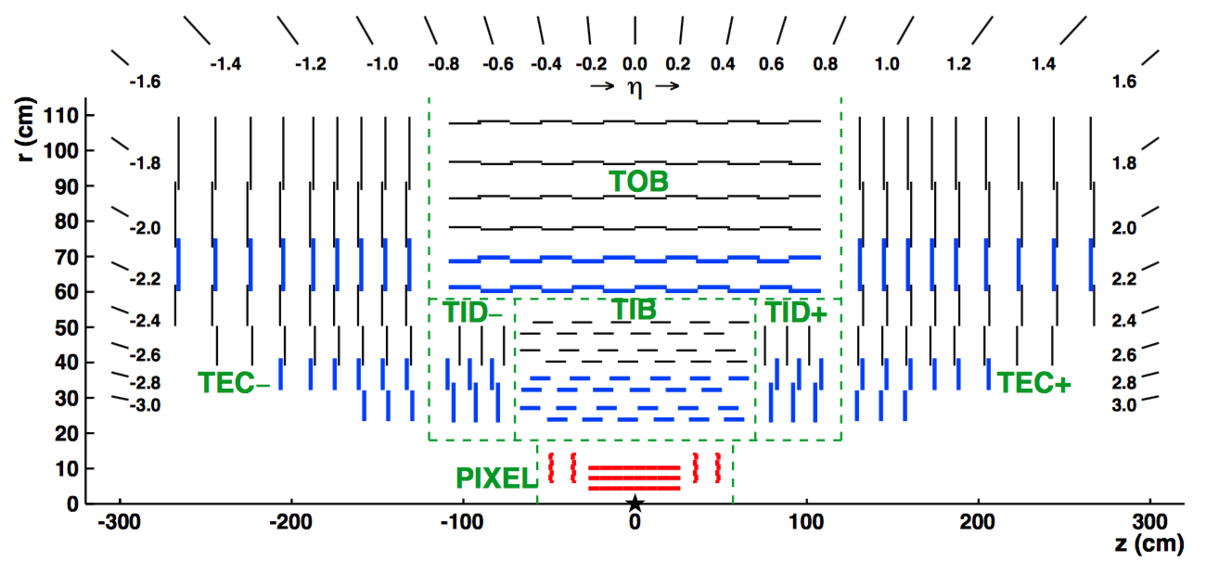
\includegraphics[width=0.7\textwidth]{2_ExperimentalSetup/Figures/imageedit_11_9317262269}
%	\caption{Schematic cross section through the CMS tracker. Each line represents a detector module. Double lines indicate back-to-back modules\cite{Chatrchyan:2008aa}.}
  \caption{Schematic cross section of the top half of the CMS tracking system in the $rz$ plane. The centre of tracker is shown with a star and corresponds to the approximate position of the proton collision point. The green dashed lines are an indication for each named tracker subsystem. The strip tracker modules that provide two-dimensional hits are shown by thin, black lines, while those able to reconstruct three-dimensional hit positions are shown by thick, blue lines. The pixel modules, shown in red, also provide three-dimensional hits. \cite{Bayatian:2006zz} }
	\label{fig:Tracker}
\end{figure}

 The tracking system consists of a cylinder of 5.8 \si{ \meter} long and 2.5 \si{ \meter} in diameter. It is immersed in a co-axial magnetic field of 3.8 \si{ \Tesla} due to the solenoid.
 As shown \fig{fig:Tracker}, the tracker is built up from a large silicon strip tracker with a small silicon pixel inside. 
 The inner region, pixel ($4.4<r<10.2$ \si{ \cm}), gets the highest flux of particles. Therefore, pixel silicon sensors of $100 \times 150$ \si{ \squared \micro \meter} is used. It consists of three cylindrical barrels that are complemented by two discs of pixel modules at each side.
 The silicon strip tracker ($20<r<116$ \si{ \cm} ) has three subdivisions. The Tracker Inner Barrel  and Discs (TIB, TID) are composed of four barrel layers accompanied by three discs at each end. The outer part of the tracker - Tracker Outer Barrel (TOB) -  consists  of 6 barrel layers. In the outer discs, there are nine discs of silicon sensors, referred to as Tracker End Caps (TEC). 
  
 
 The pixel, shown in \fig{fig:pix} has 1440 modules that cover an area of about 1 \si{ \squared \meter} and have 66 million pixels. It provides a three-dimensional position measurement of the hits arising from the interaction from charged particles with the sensors. In transverse coordinate ($r\phi$), the hit position resolution is about 10 \si{ \micro \meter}, while 20-40 \si{ \micro \meter} is obtained in the longitudinal coordinate ($z$). The sensor plane position provides the third coordinate. 
  The silicon strip trackers consists of 15 148 single sided modules placed in the TIB, TID and the first four rings of the TEC. They provide 9.3 million readout channels. In the TOB and the outer three rings of the TEC, double sided modules are used. These modules are constructed from two back-to-back single sided modules, where one module is rotated through a stereo angle.  This covers an active area of about 198 \si{ \squared  \meter}. The TIB and TID provide position measurements in $r\phi$ with a resolution of approximately 13-38 \si{ \micro \meter}, while the TOB provides a resolution of about 18-47 \si{ \micro \meter}. The resolution in the  $z$ direction is approximately 230  \si{ \micro \meter} in the TIB/TID and 530  \si{ \micro \meter} in the TOB. To allow overlay and avoid gaps in acceptance, each module is shifted slightly in $r$ or $z$ with respect to its neighbouring modules within a layer.  With this detector lay out, at least nine points per charged particle trajectory can be measured in an \abspsrap range up to 2.4.
  
  
       \begin{figure}[ht]
  	\centering
  	\begin{minipage}[b]{0.4\textwidth}
  		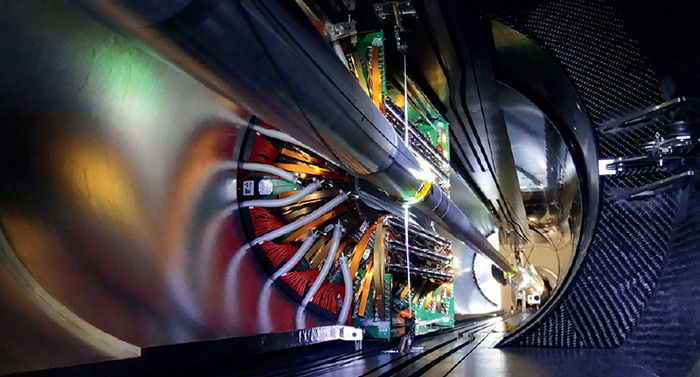
\includegraphics[width=\textwidth]{2_ExperimentalSetup/Figures/cmspixel}
  		\caption{The pixel barrel being re-installed after the Long Shutdown in 2015, around the beam pipe at CMS\cite{Christine:2024986}}
  		\label{fig:pix}
  	\end{minipage}
  	\hfill
  	\begin{minipage}[b]{0.4\textwidth}
  		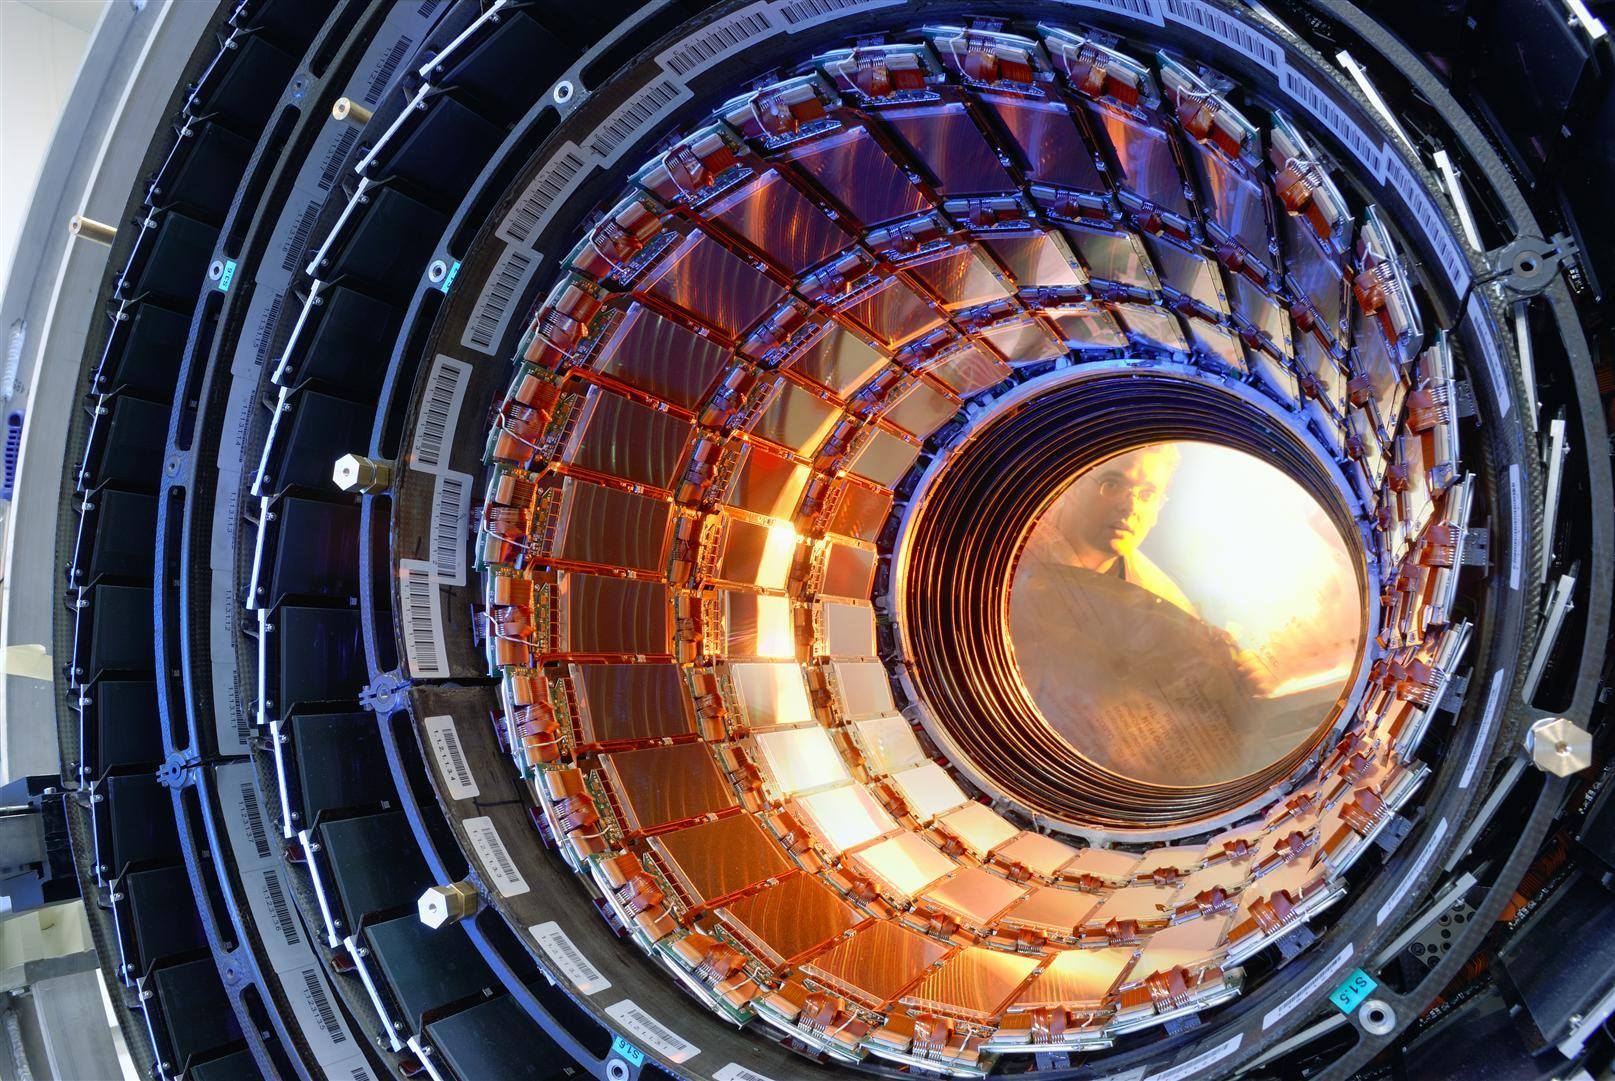
\includegraphics[width=\textwidth]{2_ExperimentalSetup/Figures/cmsbarrel}
  		\caption{First half of the inner tracker barrel, consisting of three layers of silicon modules.\cite{beautiful:1998635}}
  			\label{fig:Trackpics}
  	\end{minipage}
  
  	%	(from https://twiki.cern.ch/twiki/bin/view/CMSPublic/LumiPublicResults#Online_Luminosity_AN2 )
  \end{figure}
  
  
  
  
   During the first data taking period of the LHC (2010 to 2013), the tracker operated at +4\si{ \degree C}. With the higher LHC beam intensities from 2015 onwards, the tracker needs to be operated at much lower temperatures. This is due to the fact with intense irradiation, the doping concentration changes, the leakage current increases proportional to the fluence and the charge collection efficiency decreases due to charge trapping. Mostly the leakage current (I) is affected by the temperature change: 
   \begin{equation}
   I \propto T^2 e^{-\frac{E_g}{2kT}}, 
   \end{equation}
    where $T$ is the operating temperature, $E_g$ the band gap and $k$ the Boltzmann constant. There is approximately a factor 15 between the leakage currents at room temperatures and at $-10$ \si{ \degree C}. 
    % see http://www.hephy.at/user/friedl/diss/html/node14.html
    
    During the first long shutdown (LS1), the CMS cooling plant was refurbished\cite{running:1998606} and the fluorocarbon cooling system overhauled. To help to suppress the humidity inside the tracker, new methods for vapour sealing and insulation were applied. Furthermore, several hundred high-precision sensors are used to monitor the humidity and temperature. In order to get as dry air as possible, a new dry-gas plant provides eight times more dry gas (air or nitrogen) than during the first run, and allows regulation if the flow. As final addition, the cooling bundles outside the tracker are equipped with heater wires and temperature sensors in order to maintain safe operations above the cavern dew point For the data taking in 2015-2016, the tracker operated at $-15$\si{ \degree C}.
    
     \begin{figure}[ht]
    	\centering
    	\begin{minipage}[b]{0.3\textwidth}
    	%	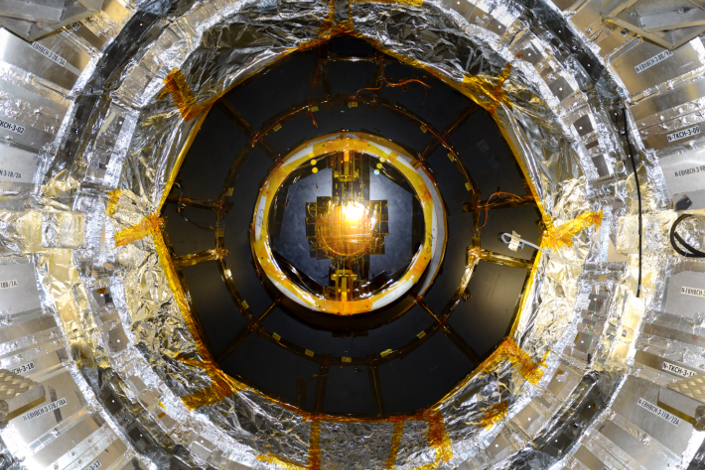
\includegraphics[width=\textwidth]{2_ExperimentalSetup/Figures/Tracker_bulkhead}
    	\includegraphics[width=\textwidth]{2_ExperimentalSetup/Figures/BHIsis}
    		\caption{Tracker bulkhead being put into closed state with insulation pieces installed during an early trial in fall 2013}
    	\end{minipage}
    	\hfill
    	\begin{minipage}[b]{0.5\textwidth}
    	%		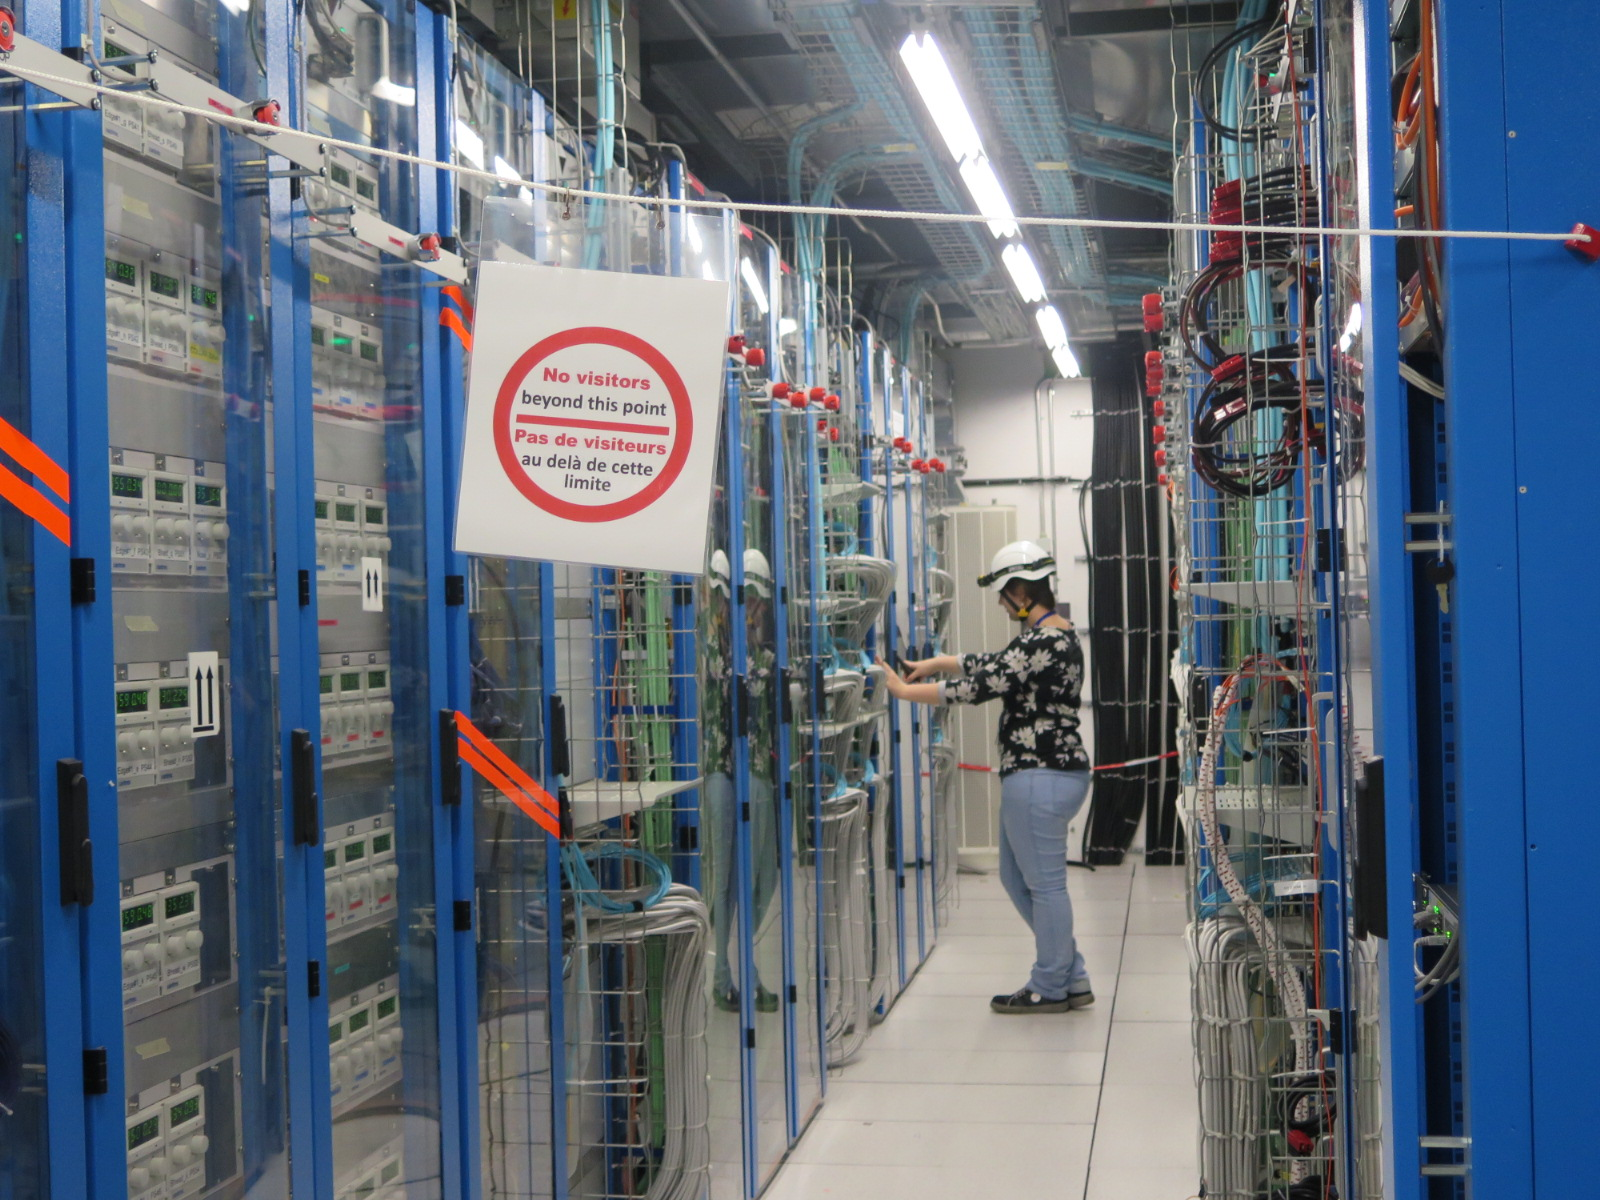
\includegraphics[width=\textwidth]{2_ExperimentalSetup/Figures/IMG_0138}
    	%	\caption{Tracker service racks containing the electronics coming from the tracking systems.}
    	
    		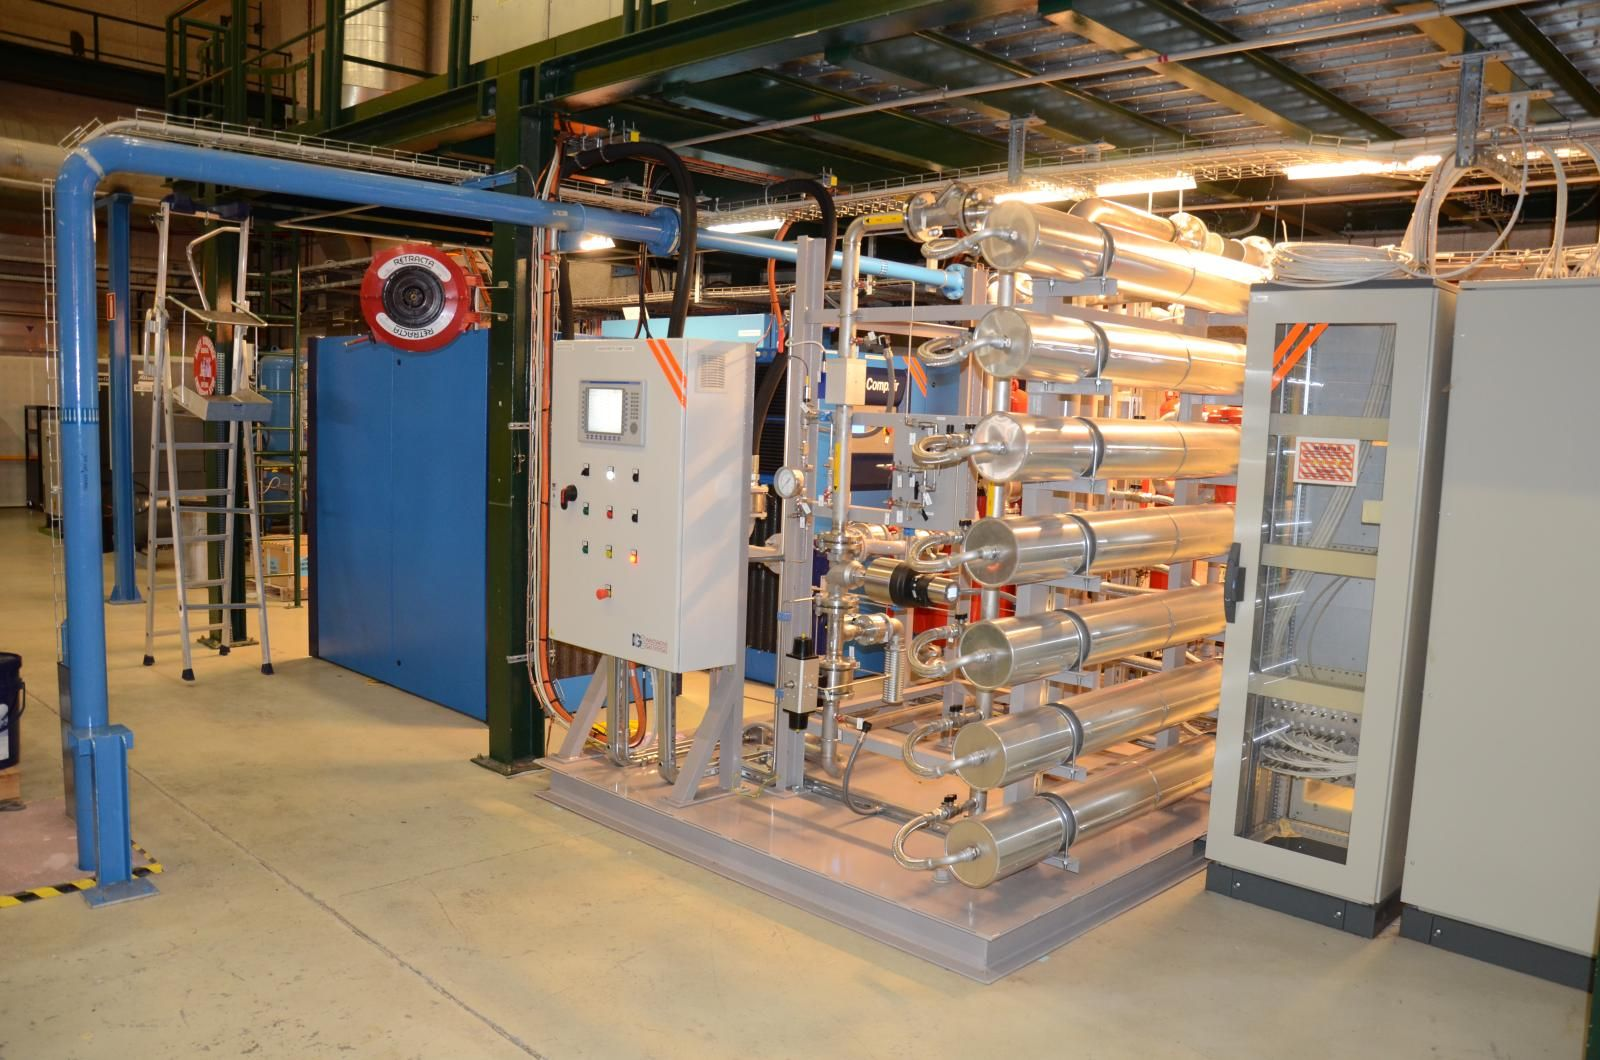
\includegraphics[width=\textwidth]{2_ExperimentalSetup/Figures/plant}
    		\caption{New Tracker high-capacity dry-gas plant with membrane separation system\cite{Pralavorio:2024977}}
    	\end{minipage}
    	\label{fig:TrackLS1}
    	%	(from https://twiki.cern.ch/twiki/bin/view/CMSPublic/LumiPublicResults#Online_Luminosity_AN2 )
    \end{figure}

\subsubsection*{Track reconstruction}
% see also https://arxiv.org/pdf/physics/0512097.pdf
% https://cds.cern.ch/record/1563583/files/ATL-PHYS-PROC-2013-206.pdf
% http://cds.cern.ch/record/1704291
An iterative tracking algorithm is responsible for the reconstruction of the tracks made by charged particles in the inner tracking system. Each iteration consists of four steps\cite{Bayatian:922757}: the track-seed generation, the pattern recognition algorithm, removal of track-hit ambiguities and a final track fit. 

The seed generation is the first step. It consists of finding reconstructed hits that are usable for seeding the subsequent track-finding algorithm. They are identified from a group of at least three reconstructed hits in the tracker, or from a pair of hits while requiring the origin of the track segment to be compatible with the nominal beam-collision point. Since the pixel has a higher granularity compared to the strip tracker, its seed generation efficiency is higher. The overall efficiency exceeds 99\%.
The second step of each iteration, the pattern recognition algorithm, uses the seeds as a starting point for a Kalman filter method~\cite{FRUHWIRTH1987444,Billoir:1989mh}. This algorithm extrapolates the seed trajectory towards the next tracker layer taking into account the magnetic field and multiple scattering effects. The track parameters are updated when a compatible hit in the next layer is found. This procedure continues until the outermost layer us reached.
Since the Kalman filter method can result in multiple tracks associated to the same seed, or different tracks sharing the same hits, a removal of ambiguities is necessary. This ambiguity resolving is done by removing tracks that are sharing too many hits from the list of track candidates. The tracks with highest number of hits or with the lowest $\chi^2$ if the track fit is kept. 
The updated track parameters are then refitted using the Kalman filter method, where all hits found in the pattern recognition step are taken into account. The fit is done twice - once outwards from the beam line towards the calorimeters, and inwards from the outermost track hit to the beam line -, improving the estimation of the track parameters. 

All hits that are unambiguously associated to the final track are removed from the list of available hits. In order to associate the remaining hits, the procedure is repeated with looser track reconstruction criteria. The use of the iterative track reconstruction procedure has a high track finding efficiency, where the fake track reconstruction rate is negligible. 
For muons, this results in a global track reconstruction efficiency exceeding 98\%, and 75-98\% for charged hadrons. Due to the lack of coverage of the two pixel discs in high \abspsrap range, the efficiency drops. 
%The resolution on the transverse momentum for a 100 \si{ \GeV} charged particle is about 2.0\% (FIX ME). 
% see https://twiki.cern.ch/twiki/bin/view/CMSPublic/TrackingPOGPlots2016
\subsubsection*{Primary vertex reconstruction}
The primary vertex reconstruction should be able to meausre the location of all proton interaction vertices in each event: the signal vertex an all vertices from pile up events. 
It consists of a vertex finding and a vertex fitting algorithm and happens in three steps. Tracks are selected  to be consistent with being produced promptly in the primary interaction by imposing requirements on track parameters\cite{Chatrchyan:1704291} By grouping reconstructed tracks according to the $z$ coordinate of their closest approach to the beam line, vertices for all interaction in the same beam crossing are found, at CMS this is done by a deterministic annealing algorithm~\cite{726788} . On top of this, a vertex fitting algorithm like the Adaptive Vertex fitter~\cite{Waltenberger:1166320}, is performed. This creates the three-dimensional primary-vertex position. With this fit, the contribution from long-lived hadron decays is reduced by down weighting the tracks with a larger distance to the vertex. The primary vertex corresponding to the highest sum of squared track transverse momenta is noted as the point of the main interaction. The resolution on the primary vertex is about 14 \si{ \micro \meter} in $r\phi$ and about 19 \si{ \micro \meter}) in the $z$ direction for primary vertices with the sum of the track $p_T > 100$ \si{ \GeV} for 2016 data taking.
% numbers from https://twiki.cern.ch/twiki/bin/view/CMSPublic/TrackingPOGPlotsICHEP2016
\subsection{Data acquisition}
% event display https://cds.cern.ch/record/2242076/files/DP2017_001.pdf
At a design luminosity of 10$^{34}$ \si{ \per \square \meter \per \second}, the proton interaction rate exceeds 1 \si{ \giga \hertz}. This makes it impossible for the CMS experiment to store all the data generated. For this, a two level trigger system has been put in place. The first level (Level-1) is a custom hardware system, while a second level (HLT) is software based running on a large farm of computers. 
In run II, with the increase in centre of mass energy and a higher luminosity a larger number of simultaneous inelastic collisions per crossing is expected with respect to run I. For this, the CMS Level-1 has been upgraded~\cite{1748-0221-12-03-C03021}. 

\subsubsection*{CMS Level-1 trigger}
The Level-1 trigger has to be a flexible, maintainable system, capable of adapting to the evolving physics programme of CMS~\cite{Khachatryan:2016bia}. Its output rate is restricted to 100 \si{ \kilo \hertz} imposed by the CMS readout electronics. It is implemented by custom hardware and selects events containing candidate objects - eg ionization deposits consistent with a muon, or energy clusters corresponding to an electron / photon / tau lepton / missing transverse energy / jet. Collisions with large momenta can be selected by using scalar sum of the transverse momenta of the jets. 

\begin{comment}
\begin{figure}[h]
	\centering
	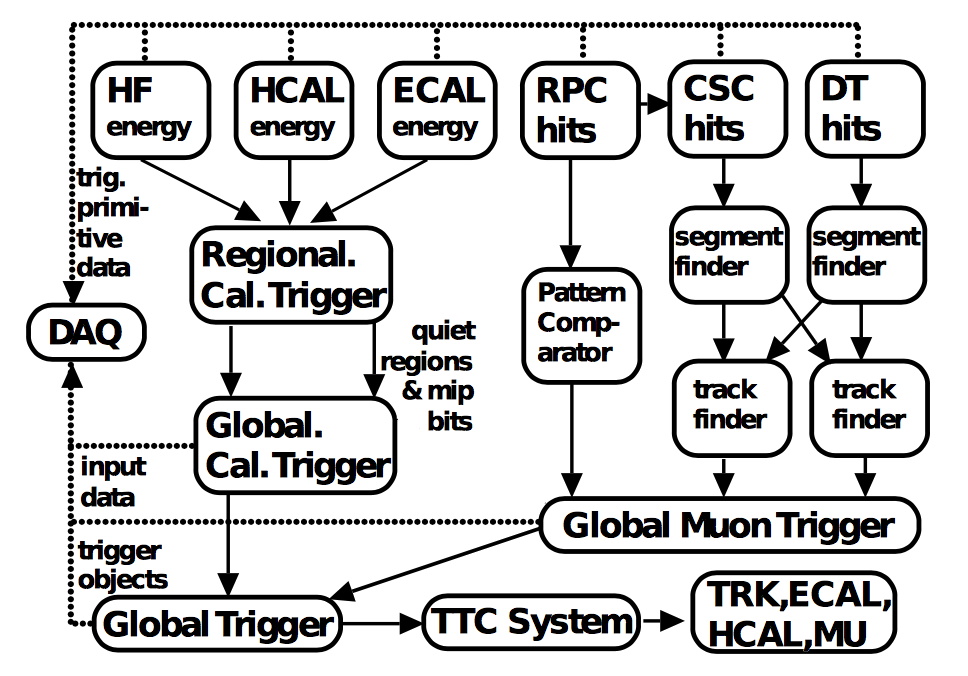
\includegraphics[width=0.5\linewidth]{2_ExperimentalSetup/Figures/imageedit_13_6388071145}
	\caption{The CMS level 1 trigger system for run I. Data from the calorimeters are processed regionally (RCT) ad the globally (GCT). Data from the muon chambers are processed via a global muon trigger (GMT). A global trigger (GT) combines the GCT and GMT, making a trigger decision. Th data acquisition system (DAQ) reads data from the tracker (TRK) via the trigger, timing  and control (TTC) system \cite{Khachatryan:2016bia}.}
	\label{fig:level1}
\end{figure}
\end{comment}

By buffering the raw data from the CMS subdetectors in front-end drivers, the level-1 trigger has a pipeline memory of 3.2 \si{ \micro \second} to decide whether to keep an event or reject it. 
%In \fig{fig:level1} the structure of the trigger is shown. 
The trigger primitives (TP) from the calorimeters and muon detectors are processed in several steps and combined into a global trigger. This information is then combined with the input from the other subsystems. The seperate inouts are synchronized to each other and the LHC orbit clock and sent to th eglobal trigger module. Here, level-1 trigger algorithms are performed within 1 \si{ \micro \second} to decide whether to  keep the event. 

For run II, all hardware, software, databases and the timing control system have been replaced. The main changes are that the muon system now uses the redundancy of three muon detector system earlier to make a high resolution muon trigger. The calorimeter system isn't bound any more for streaming data the data and the global trigger has more level-1 trigger algorithms. 
% see https://indico.cern.ch/event/432527/contributions/1072399/attachments/1320545/1980311/ichep2016.pdf

\subsubsection*{CMS HLT trigger}
The HLT is an array of commercially available computers with programmable menu that has output rate of on average 400 \si{ \hertz} for off-line event storage.
The data processing is based on a HLT path. This is a  set of algorithmic steps to reconstruct objects and make selections on them.  Here, the information of all sub detectors can be used to perform algorithms on higher level reconstructed objects. 
(FIXME: tracker in hlt or already in L1? )
\subsection{CMS computing model}
The selected data is stored, processed and dispersed via the Worldwide Large Hadron Collider GRID (WLCG)\cite{Grandi:814248,Eck:840543}. This has a tiered structure that function as a single, coherent system:. 

At CERN, a single Tier-0 is located. The raw data collected by CMS is archived here, and a first reconstruction of the data is done. This data is then in a file format usable for physics analysis. Furthermore, it is able to reprocess data when new calibrations are made available. The Tier-0 site distributes this data to a total of seven Tier-1 centres. They carry out data reprocessing and store real data as well as simulated  data. The Tier-1 further distribute the data to over 50 Tier-2 centres. These make the data accessible for physics analysis and are also being used for the production of simulated data. This data is accessible for  physicists around the world. 


\chapter{Analysis techniques}
\todo{Write introduction to this chapter}
\section{Hadron collisions at high energies}
In hadron collisions at as sufficiently high momentum transfer, all partons can be approximated as free  making it possible to treat hadron-hadron scattering as a single parton-parton interaction. The momentum of the parton can then be expresses as a fraction of the hadron momentum 
\begin{equation}
 \vec{p}_{\mathrm{parton}} = x \vec{p}_{\mathrm{hadron}}, 
\end{equation}
where $x$ is referred to as the Bj\"orken scaling variable. The interaction $\Pproton_{\mathrm{A}} \Pproton_{\mathrm{B}} \rightarrow \mathrm{X}$ can then be factorised in terms of partonic cross sections $\hat{\sigma}_{\mathrm{ij}\rightarrow\mathrm{X}}$~\cite{Collins:1989gx}
\begin{equation}
 \sigma_{\mathrm{p}_{\mathrm{A}}\mathrm{p}_{\mathrm{B}}\rightarrow\mathrm{X}} = \sum \limits_{\mathrm{ij}} \iint dx_1 dx_2  \: f_{\mathrm{i}}^{\mathrm{A}}(x_{\mathrm{1}},Q^2)f_{\mathrm{j}}^{\mathrm{B}}(x_{\mathrm{2}},Q^2) {d\hat{\sigma}_{\mathrm{ij}\rightarrow\mathrm{X}}}, 
 \label{eq:cross}
 \end{equation}
where i and j are the partons resolved from protons A and B,  $f_{\mathrm{i}}(x_{\mathrm{i}},Q^2)$ the parton density functions (PDF), and $Q^2$ the factorisation scale more commonly denoted as \muF. The factorisation scale is the scale at which the hadronic interaction can be expressed as a product of the partonic cross section and the process independent PDF. In \fig{fig:factoscale}, the kinematic regions in $x$ and \muF\ are shown for fixed target and collider experiments.
\begin{figure}
	\centering
	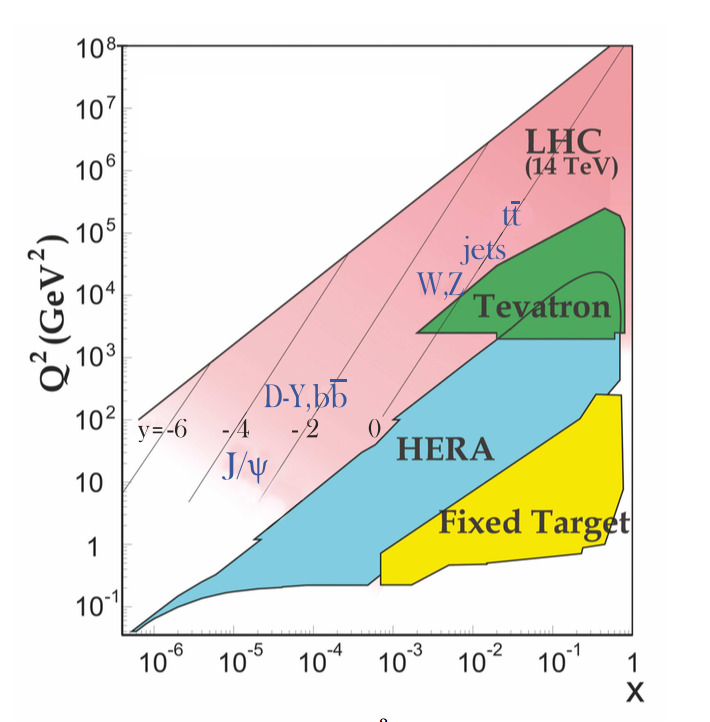
\includegraphics[width=0.5\linewidth]{3_Analysis_techniques/Figures/factoscale}
	\caption{Kinematic regions in momentum fraction $x$ and factorisation scale $Q^2$ probed by fixed-target and collider experiments. Some of the final states accessible at the LHC are indicated in the appropriate regions, where $y$ is the rapidity. In this figure, the incoming partons have $x_{1,2} = (M/14 \TeV)e^{\pm y}$ with $Q = M$ where $M$ is the mass of the state shown in blue in the figure. For example, exclusive J$/\psi$ and $\Upsilon$ production at high $|y|$ at the LHC may probe the gluon PDF down to $x \sim  10^{-5}$. Figure taken from \cite{PDG}.}
	\label{fig:factoscale}
\end{figure}
%https://arxiv.org/pdf/1206.7024.pdf voor goede info



 The parton density functions (PDF)~\cite{Placakyte:2011az,Ball2015,Butterworth:2015oua} give the momentum distribution of the proton amongst its partons at an energy scale \muF.  
  These function can not be determined from first principles and have to obtained from global fits to data. The PDFs are obtained from measurements on deep inelastic scattering using lepton-proton collision by the HERA collider~\cite{Abramowicz:1998ii}, supplemented with proton-antiproton collisions from Tevatron at Fermi lab~\cite{Holmes:2011ey}, and proton collision data from the ATLAS, CMS and LHCb collaborations at the LHC (Run 1)~\cite{Rojo:2015acz}. These measurements are included in global PDF sets known as the \texttt{PDF4LHC} recommendation~\cite{Butterworth:2015oua}. From their measurement at scale \muF\ these PDFs can be extrapolated using the DGLAP equations \todocite. The PDFs are used to calculate the cross section of a certain process and are therefore used as input for the Monte Carlo generators used to make the simulated data samples at the LHC. 
%https://amva4newphysics.wordpress.com/2016/03/10/the-inner-life-of-protons-and-artificial-neural-networks/
In the framework of this thesis, the NLO \texttt{PDF4LHC}15\_100 set is used. This set is an envelope of three sets, \texttt{CT14}, \texttt{MMHT2014} and \texttt{NNPDF3.0}~\cite{Butterworth:2015oua}. In \fig{fig:nnpdf30} the dependency of the PDFs on the momentum fraction $x$ is shown for the \texttt{NNPDF3.0} set on hadronic scale ($\muF^2 = (10\GeV)^2$ and LHC scale ($\muF^2 = (10^4\GeV)^2$. For most values of the momentum fraction, the gluon density dominates, meaning that it is easier to probe muons than the quarks. For $x$ close to one, the parton densities of the up and down quarks (the valence quarks of the proton) dominate over the gluon density. The charm, anti-up, and anti-down quarks have lower densities in general since those are sea quarks which originate in the proton only through gluon splitting. 
The resolution scale $Q^2$ is typically taken to be the energy scale of the collision. For the top quark pair production a scale of $Q^2=(350\: \GeV)^2$ is chosen, meaning that the centre-of-mass energy of the hard interaction is about twice the top quark mass.
\begin{figure}[htbp]
	\centering
	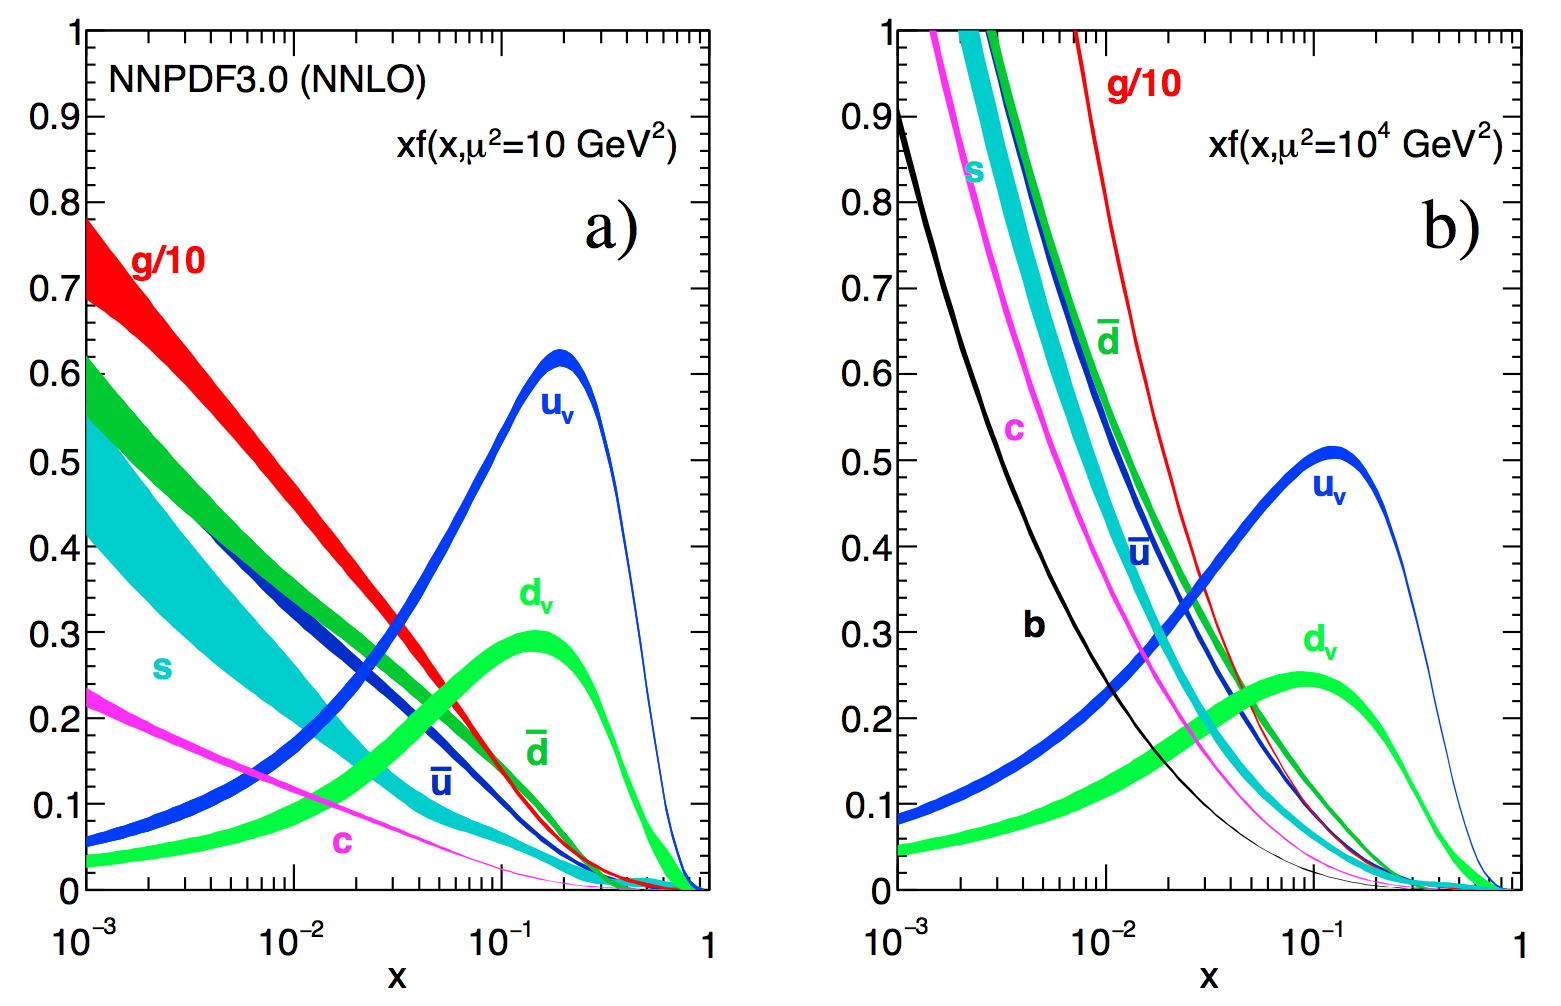
\includegraphics[width=0.7\linewidth]{3_Analysis_techniques/Figures/NNPDF30}
	\caption{The momentum fraction $x$ times the parton distribution functions $f(x)$, where $f=\Pup_{\mathrm{v}}, \Pdown_{\mathrm{v}} ,\APup,\APdown,\Pstrange,\Pcharm,$ or \Pgluon\ as function of the momentum fraction obtained in the NNLO \texttt{NNPDF3.0} global analysis at factorisation scales $\mu^2 = 10 \: \GeV^2$ (left) and $\mu^2=10^4 \: \GeV^2$ (right), with $\alpha_{\mathrm{S}}(M^2_{\PZ}) = 0.118$. The gluon PDF has been scaled down by a factor of 0.1. Figure taken from \cite{PDG}.}
	%http://pdg.lbl.gov/2017/reviews/rpp2016-rev-structure-functions.pdf
	% The higher value of the resolution scale $Q^2$, the smaller distances that are probed in the proton.
	\label{fig:nnpdf30}
\end{figure}
The uncertainty on the parton distributions is evaluated using the Hessian technique~\cite{Pumplin:2001ct}, where a matrix with a dimension identical to the number of free parameters needs to be diagonalised. In the case of \texttt{PDF4LHC}15\_100 set, this translates into 100 orthonormal eigenvectors and 200 variations of the PDF parameters in the plus and minus direction. 
%https://www.hep.ucl.ac.uk/pdf4lhc/LesHouches2016-PDF4LHC.pdf
%https://indico.cern.ch/event/525605/contributions/2152733/attachments/1267702/1877336/TOP_PAG_3_05_16_PDFs.pdf

At high energies divergences can appear from quantum fluctuations. For the theory still to be able to describe the experimental regime, a renormalization scale \muR\ is used to redefine physical quantities A consequence of this method is that the coupling constants will run as function of \muR. Beyond this scale, the high energy effects such as the loop corrections to propagators (self energy) are absorbed in the physical quantities through a renormalization of the fields. In particular the running behaviour of the strong coupling constant\footnote{The strong coupling constant is defined as $\alpha_{\mathrm{S}} = \frac{g_\mathrm{S}^2}{4\pi}$. } $\alpha_{\mathrm{S}}$ is found to be 
\begin{equation}
	\alpha_{\mathrm{S}} = \frac{\alpha_{\mathrm{S}}(\mu_0^2)}{1 + \alpha_{\mathrm{S}}(\mu_0^2) \frac{33 - 2 n_{\mathrm{f}}}{12 \pi}\mathrm{ln}\left(\frac{|\muR^2|}{\mu_0^2}\right)}, 
	\label{eq:couplingstrength}
\end{equation}
with $n_{\mathrm{f}}$ the number of quarks and $\mu_0$ the reference scale on which the coupling is known. The current world average of the strong coupling constant at the \PZ boson mass is $\alpha_{\mathrm{S}}(\muF = \mZ) = 0.1181 \pm 0.0011$~\cite{PDG}. From  \eq{eq:couplingstrength} one can see easily that the coupling strength decreases with increasing renormalization scale, this known as asymptotic freedom. Additionally, following the behaviour of $\alpha_{\mathrm{S}}(\muR^2)$, a limit $\Lambda_{\mathrm{QCD}} \approx 200 \: \MeV$ is found for which $\alpha_{\mathrm{S}}$ becomes larger than one. Under this limit, the perturbative calculations of observables can no longer be done.
% Mandl and shaw pagina 352!



%The cross section $\sigma$ of scattering process with a flux\footnote{This entity is more commonly referred to as Luminosity.} $\lumi= \rho v$ of incoming particles with particle density $\rho$ and velocity $v$ is defined as the number of interactions per unit density ($\rho=1$)\footnote{The cross section is usual expressed in barn, $1b = 10^{-28}\m^2$. The number of interactions per time is given by $\frac{dN}{dt} = \lumi \sigma$}. 
Cross sections be written in terms of interacting vertices contributing to the matrix element (ME) originating from elements of a perturbative series~\cite{Mandl:1236742}, allowing them to be expanded as a power series of the coupling constant $\alpha$ 
\begin{equation}
 \sigma  = \sigma_{\mathrm{LO}} \left(1 + \left(\frac{\alpha}{2\pi}\right)\sigma_1  + \left(\frac{\alpha}{2\pi}\right)^2\sigma_2 + ...\right).
\end{equation}
Leading order (LO) accuracy contains the minimal amount of vertices in the process, then depending on where the series is cut off one speaks of next-to-leading order (NLO), or next-to-next-to-leading order (NNLO) accuracy in $\alpha$. Predictions including higher order correction tend to be less affected by theoretical uncertainties originating from a variation of the chosen renormalization and factorisation scales. 
% zie thesis matthias p 21 bovenaan

\section{Event generation}
In order to compare reconstructed data with theoretical predictions, collision events are generated and passed through a simulation of the CMS detector and an emulation of its readout. For the detector simulation, a so-called Full Simulation package~\cite{1742-6596-396-2-022003,1742-6596-664-7-072022}  based on the \Geant4 toolkit~\cite{AGOSTINELLI2003250} is employed. It allows a detailed simulation of the interactions of the particles with the detector material. 
\subsection{Fundamentals of simulating a proton collision}
The procedure of to generate $\Pproton\Pproton \rightarrow \mathrm{X}$ events can be subdivided into sequential steps~\cite{Seymour:2013ega,Sjostrand:2009ad,Hoche:2014rga}, as shown in \fig{fig:ppcollision}.
\begin{figure}[htbp]
	\centering
	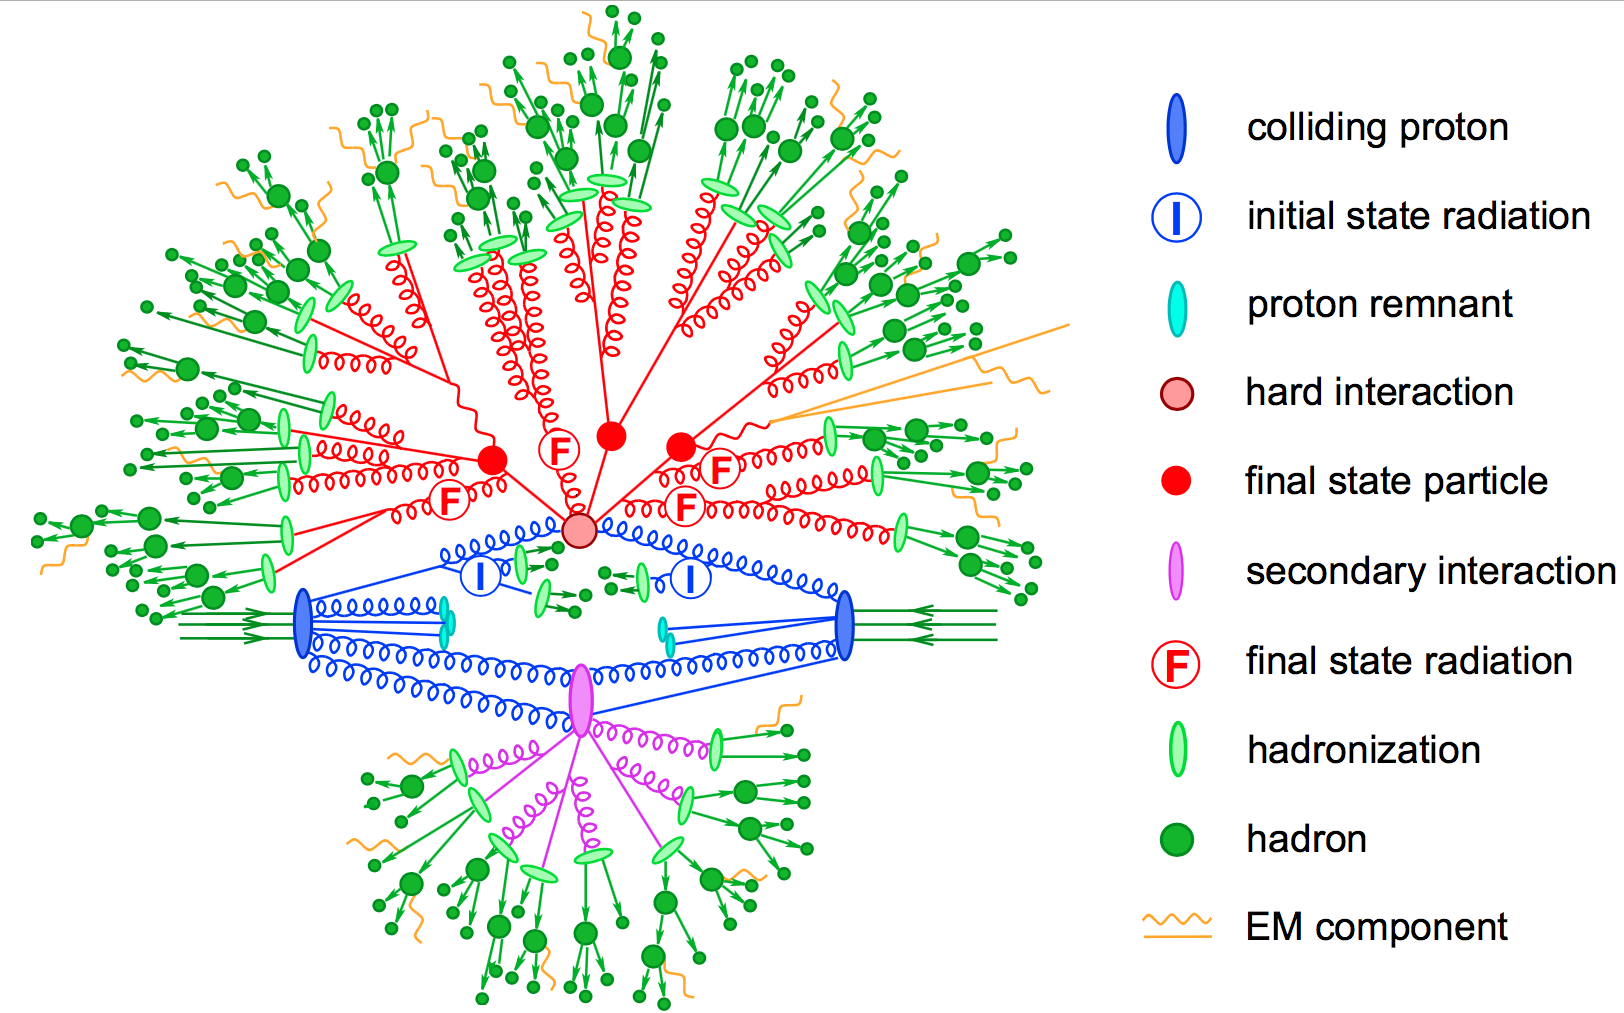
\includegraphics[width=1.\linewidth]{3_Analysis_techniques/Figures/MCeventwithlegend}
	\caption{Sketch of a hadron collision as simulated by a Monte-Carlo event generator. The red blob in the centre represents the hard collision, surrounded by a tree-like structure representing Bremsstrahlung as simulated by parton showers. The purple blob indicates a secondary hard scattering event. Parton-to-hadron transitions are represented by light green blobs, dark green blobs indicate hadron decays, while yellow lines signal soft photon radiation. Figure taken from~\cite{Hoche:2014rga}.}
	\label{fig:ppcollision}
\end{figure}

The interaction of two incoming protons is often soft and elastic leading to events that are not interesting in the framework of this thesis. More intriguing are the hard interaction between two partons from the incoming protons. The matrix elements   of a hard scattering process of interest is the starting point of the generation of events. Monte Carlo techniques are used to sample the corresponding cross section integral and the resulting sample of events reflect the probability distribution of a process over its final state phase space. After obtaining the sample of events of the hard interaction, a parton shower (PS) program is used to simulate the hadronisation of final state partons into hadrons which then  decay further. Additionally, radiation of soft gluons or quarks from initial or final state partons is simulated. These are respectively referred to as initial state radiation (ISR) or final state radiation (FSR). Contributions from soft secondary interactions, the so-called underlying event (UE), and colour reconnection effects are also taken into account. \todo{Should I add more details?}
A brief overview of the employed programs used for the event generation of the signal and main background processes used in the search presented in the thesis are given in \Sec{sec:programs}.

\subsection{Programs for event generation}
\label{sec:programs}
The \texttt{FEYNRULES} package~\cite{Alloul:2013bka} allows the calculation of  the Feynman rules in momentum space for any quantum field theory model. By use of a Lagrangian, the set of Feynman rules associated with this Lagrangian are calculated. Via the \UFO\ (UFO)~\cite{Degrande:2011ua} the results are then passed to matrix element generators. 


The \MG\  program~\cite{Alwall:2011uj} is used to interpret the physics model and calculate the corresponding Feynman diagrams and matrix elements. After this, \ME~\cite{Mangano:2006rw} is used to calculate the corresponding partons. These generated parton configurations are then merged with \Pythia~\cite{Sjostrand2015159,Sjostrand:2006za,Sjostrand:2014zea} parton showers using the MLM merging scheme~\cite{Alwall:2007fs}. 

The \aMCMG\ program~\cite{Alwall:2014hca} combines the LO \MG~\cite{Alwall:2011uj} and the \aMC\ program into a common framework. This combination supports the generation of samples at LO or next to NLO together with a dedicated matching to parton showers  using the MLM~\cite{Alwall:2007fs} or FXFX~\cite{Frederix:2012ps} schemes respectively. The FXFX scheme produces a certain fraction of events with negative weights originating from the subtraction of amplitudes that contain additional emissions from the NLO matrix element to prevent double-counting.
%or MC$@$NLO~\cite{Frederix:2012ps}  \todo{MC$@$NLO voor ME generator }



The \Powheg\ box (versions 1,2)~\cite{Alioli2010,1126-6708-2009-09-111,1126-6708-2007-11-070,Alioli:2010xd,Frixione:2007vw,Nason:2004rx} contains predefined implementations of various processes at NLO. It applies the \Powheg\ method for ME- to PS- matching, where the hardest radiation generated from the ME has priority over subsequent PS emission to remove the overlap with the PS simulation.

The \JHU\ generator (version 7.02)~\cite{Gritsan:2016hjl,Anderson:2013afp,Bolognesi:2012mm,Gao:2010qx} is used to generate the parton level information including full spin and polarization correlations. It is commonly used for studying the spin an parity properties of new resonances such as $\mathrm{ab}\rightarrow\mathrm{X}\rightarrow \mathrm{VV}$, where $\mathrm{V} = \PZ, \PW, \Pphoton)$. 

The generation of events from processes involving the production and decay of resonances creates a computational heavy load, especially at NLO. The narrow width approximation the resonant particle is assumed to be on-shell. This makes the production and decay amplitude factorize, allowing to perform the simulation of the production and decay of heavy resonances like top quarks or Higgs bosons to be performed in separate steps. The \MS\ program~\cite{Artoisenet:2012st} extends this approach and accounts for off-shell effects through a partial reweighting of the events. Additionally, spin correlation effects between production and decay products are taken into account. 

The \Pythia\ program (versions 6,8)~\cite{Sjostrand2015159,Sjostrand:2006za,Sjostrand:2014zea} generates events of various processes at LO. Usually in the analysis, it is however only used for its PS simulation and it is interfaced with other LO and NLO event generators to perform subsequent parton showering, hadronisation, and simulation of the underlying event.  In this thesis the underlying event tunes~\cite{Khachatryan2016}  are the CUETP8M2T4, CUETP8M1 and CUETP8M2. 





The detector response is simulated via the \Geant 4~\cite{AGOSTINELLI2003250} program. This program tracks the particles through the detector material via a detailed description of the detector and generates several hits throughout several sensitive layers. 
In addition, the response of the detector electronics to these hits are simulated. 


\subsection{Generating FCNC top-Z interactions}
The FCNC processes are generated by interfacing the Lagrangian in \eq{eq:EFTlag} with \aMCMG\ by means of the \FR\ package and its  \UFO\ format.  The complex chiral parameters are arbitrary chosen to be $f^{\mathrm{L}}_{\mathrm{X}\Pquark} = 0$ \todo{Why LH and not RH?} and  $f^{\mathrm{R}}_{\mathrm{X}\Pquark} = 1$. The signal rates are estimated by use of the \aMCMG\ program for estimating the partial widths. The anomalous couplings are left free to float for this estimation, and only one coupling allowed to be non-vanishing at a time. The results are presented in \tab{tab:partialwidths}.
\begin{table}[htbp]
	\centering
	\caption{Leading order partial widths related to the anomalous decay modes of the top quark, where the new physics scale $\Lambda$ is given in \GeV.}
	\begin{tabular}{ccll}
		\toprule
		Anomalous coupling & vertex & \multicolumn{2}{c}{Partial decay width  (\GeV) }\\ 
		\midrule
		\multirow{2}{*}{\kgqtl} & \Ptop\Pgluon\Pup      &  3.665220 $10^{5}$   & $\left( \kappa_{\Ptop\Pgluon\Pup} / \Lambda \right)^2$ \\
		                    & \Ptop\Pgluon\Pcharm       &  3.664620 $10^{5}$   & $\left( \kappa_{\Ptop\Pgluon\Pcharm} / \Lambda \right)^2$ \\
	    \multirow{2}{*}{\kfqtl} & \Ptop\Pphoton\Pup     &  1.989066 $10^{4}$   & $\left( \kappa_{\Ptop\Pphoton\Pup} / \Lambda \right)^2$ \\
		                    & \Ptop\Pphoton\Pcharm      &  1.988904 $10^{4}$   & $\left( \kappa_{\Ptop\Pphoton\Pcharm} / \Lambda \right)^2$    \\
		\multirow{2}{*}{\kZqtl} & \Ptop\PZ\Pup          &  1.637005 $10^4$     & $\left( \kappa_{\Ptop\PZ\Pup} / \Lambda \right)^2$     \\
		                    & \Ptop\PZ\Pcharm           &   1.636554 $10^4$    & $\left( \kappa_{\Ptop\PZ\Pcharm} / \Lambda \right)^2$  \\
		\multirow{2}{*}{\zZqt} & \Ptop\PZ\Pup           &   1.685134 $10^{-1}$ & $\left( \zeta_{\Ptop\PZ\Pup}  \right)^2$ \\
		                    & \Ptop\PZ\Pcharm           &   1.684904 $10^{-1}$ & $\left( \zeta_{\Ptop\PZ\Pcharm} \right)^2$ \\
	    \multirow{2}{*}{\eHqt} & \Ptop\PHiggs\Pup       &   1.904399 $10^{-1}$ & $\left( \eta_{\Ptop\PHiggs\Pup}  \right)^2$  \\
		                    & \Ptop\PHiggs\Pcharm       &   1.904065 $10^{-1}$ & $\left( \eta_{\Ptop\PHiggs\Pcharm}  \right)^2$ \\
			\bottomrule
	\end{tabular} 
	\label{tab:partialwidths}
\end{table}
The anomalous single top cross sections are calculated by convolution of the hard scattering matrix elements with the LO order set of \CTEQ 6 partons densities~\cite{Pumplin:2002vw}. The NLO effects are modelled by multiplying each LO cross section by a global $k$-factor. The LO single top production cross section and the global $k$-factors for the top-\PZ production are shown in \tab{tab:STx}. The hard scattering events are then matched to parton showers to \Pythia\ to account for the simulation of the QCD environment relevant for hadronic collisions. 
\begin{table}[htbp]
	\centering
	\caption{Leading order single top production cross section for $\Pproton\Pproton \rightarrow \tZ$ or \tbarZ, where the new physics scale is given in \GeV. The NLO $k-$factors~\cite{Zhang:2011gh} are given in the last column.}
	\begin{tabular}{cllc}
		\toprule
	   Anomalous coupling & \multicolumn{2}{c}{Cross section (\pb)} &  NLO $k-$factor \\ 
		\midrule
	    $\kappa_{\Ptop\Pgluon\Pup} / \Lambda $     &  3.272 $10^7$  & $\left( \kappa_{\Ptop\Pgluon\Pup} / \Lambda \right)^2$ & 1.00 \\
	    $\kappa_{\Ptop\Pgluon\Pcharm} / \Lambda $  &  3.021 $10^6$  & $\left( \kappa_{\Ptop\Pgluon\Pcharm} / \Lambda \right)^2$ & 1.00 \\
	    $\kappa_{\Ptop\Pphoton\Pup} / \Lambda $    &  2.260 $10^5$  & $\left( \kappa_{\Ptop\Pphoton\Pup} / \Lambda \right)^2$ & 1.00 \\
	    $\kappa_{\Ptop\Pphoton\Pcharm} / \Lambda $ &  2.654 $10^4$  & $\left( \kappa_{\Ptop\Pphoton\Pcharm} / \Lambda \right)^2$ & 1.00 \\
	    $\kappa_{\Ptop\PZ\Pup} / \Lambda $         &  1.728 $10^6$  & $\left( \kappa_{\Ptop\PZ\Pup} / \Lambda \right)^2$ & 1.40 \\
	    $\kappa_{\Ptop\PZ\Pcharm} / \Lambda $      &  2.040 $10^5$  & $\left( \kappa_{\Ptop\PZ\Pcharm} / \Lambda \right)^2$ & 1.40 \\
	    $\zeta_{\Ptop\PZ\Pup} $                    &  7.484         & $\left( \zeta_{\Ptop\PZ\Pup} \right)^2$ & 1.40 \\
	    $\zeta_{\Ptop\PZ\Pcharm} $                 &  1.038         & $\left( \zeta_{\Ptop\PZ\Pcharm}  \right)^2$ & 1.40 \\
       \bottomrule
	\end{tabular} 
	\label{tab:STx}
\end{table}

The top pair cross sections are derived from the \SM\ \ttbar\ cross section, calculated with \aMCMG\ at NLO ($\sigma_{\ttbar} = 6.741 \; 10^{2} \pb$), and considering the decay $\ttbar \rightarrow (\Pbottom \PWpm)(\mathrm{X}\Pquark\Ptop)$. The branching ratio $\BR(\Ptop \rightarrow \Pbottom\PWpm)$ is assumed to be equal to one and the FCNC branching ratio is calculated as 
\begin{equation}
 \BR(\Ptop \rightarrow \Pquark\mathrm{X}) = \frac{ \Gamma_{\Ptop \rightarrow \Pquark\mathrm{X}} }{\Gamma_{\Ptop}^{\mathrm{SM}} + \Gamma_{\Ptop}^{\mathrm{FCNC}} }
 		\approx  \frac{ \Gamma_{\Ptop \rightarrow \Pquark\mathrm{X}} }{\Gamma_{\Ptop}^{\mathrm{SM}}} , 
\end{equation}
where $\Gamma_{\Ptop \rightarrow \Pquark\mathrm{X}}$ is given in \tab{tab:partialwidths}, and the assumption $ \Gamma_{\Ptop}^{\mathrm{FCNC}} \ll \Gamma_{\Ptop}^{\mathrm{SM}}$ is made \todo{these partial widths are at LO, how does this relate to NLO that is used? Or is there no difference?}. In \tab{tab:TTx}  the resulting NLO cross sections for the top-Z FCNC interactions are given.  
\begin{table}[htbp]
	\centering
	\caption{ Next to leading order top pair cross section for the top-Z FCNC interactions with with a full leptonic decay. }
	\begin{tabular}{ccll}
		\toprule
		Anomalous coupling & Process &   \multicolumn{2}{c}{Cross section (\pb)}  \\ 
		\midrule
\multirow{2}{*}{$\kappa_{\Ptop\PZ\Pup}/\Lambda$} & $\ttbar \rightarrow (\Pbottom \Pleptonplus\Pneutrino) (\APup \Pleptonplus \Pleptonminus)$ & 2.727008 $10^5$  & $\left( \kappa_{\Ptop\PZ\Pup}/\Lambda \right)^2$ \\
& $\ttbar \rightarrow (\APbottom \Pleptonminus\APneutrino) (\Pup \Pleptonplus \Pleptonminus)$ & 2.727008 $10^5$  & $\left( \kappa_{\Ptop\PZ\Pup}/\Lambda \right)^2$ \\
\multirow{2}{*}{$\kappa_{\Ptop\PZ\Pcharm}/\Lambda$} & $\ttbar \rightarrow (\Pbottom \Pleptonplus\Pneutrino) (\APcharm \Pleptonplus \Pleptonminus)$ &2.726257$10^5$  & $\left( \kappa_{\Ptop\PZ\Pcharm}/\Lambda \right)^2$ \\
 & $\ttbar \rightarrow (\APbottom \Pleptonminus\APneutrino) (\Pcharm \Pleptonplus \Pleptonminus)$ & 2.726257 $10^5$  & $\left( \kappa_{\Ptop\PZ\Pcharm}/\Lambda \right)^2$ \\
\multirow{2}{*}{$\zeta_{\Ptop\PZ\Pup}$} & $\ttbar \rightarrow (\Pbottom \Pleptonplus\Pneutrino) (\APup \Pleptonplus \Pleptonminus)$ & 2.827184   & $\left( \zeta_{\Ptop\PZ\Pup}\right)^2$ \\
 & $\ttbar \rightarrow (\APbottom \Pleptonminus\APneutrino) (\Pup \Pleptonplus \Pleptonminus)$ & 2.827184   & $\left( \zeta_{\Ptop\PZ\Pup}\right)^2$ \\
\multirow{2}{*}{$\zeta_{\Ptop\PZ\Pcharm}$} & $\ttbar \rightarrow (\Pbottom \Pleptonplus\Pneutrino) (\APcharm \Pleptonplus \Pleptonminus)$ & 2.806801  & $\left( \zeta_{\Ptop\PZ\Pcharm}\right)^2$ \\
& $\ttbar \rightarrow (\APbottom \Pleptonminus\APneutrino) (\Pcharm \Pleptonplus \Pleptonminus)$ & 2.806801  & $\left( \zeta_{\Ptop\PZ\Pcharm}\right)^2$ \\
		\bottomrule
	\end{tabular} 
	\label{tab:TTx}
\end{table}



\subsection{Generating \SM\  background events}
The SM \tZq events were generated using the \aMCMG\ generator, interfaced with \Pythia\ version 8.2~\cite{Sjostrand:2014zea}  for parton showering and hadronisation. The \WZ+jets, \ttZ, \tZq, and \ttW\ samples are produced using the \aMCMG (version 5.222)~\cite{Alwall:2014hca}, which includes up to one hadronic jet at next to leading order (NLO) QCD accuracy. Other minor background (e.g. \WW, \ZZ, \tWZ\ and \ttH) are simulated using different generators such as \MG~\cite{Alwall:2011uj},\MS~\cite{Artoisenet:2012st} and \JHU~\cite{Gritsan:2016hjl,Anderson:2013afp,Bolognesi:2012mm,Gao:2010qx}. All events are interfaced to \Pythia\ for parton shower and hadronisation. 

The complete list of \SM\ samples is given in Table \ref{tab:samples} \todocite, along with their cross sections. The cross sections without a reference are coming from the generator with which the sample has been made, for some of them the uncertainties are provided by the Generator Group. For each MC sample, the integrated luminosity that the sample represents is estimated as the number of simulated events divided by the cross section of the generated process. For processes generated with \aMCMG, the effective number of simulated events is used, taking into account positive and negative event weights. The correction factor for those events is defined as
\begin{equation}
\mathrm{C} = \frac{\textnormal{Nb. of pos. weights} + \textnormal{Nb. of neg. weights}}{\textnormal{Nb. of pos. weights} - \textnormal{Nb. of neg. weights}} \times \textnormal{mc baseweight}
\end{equation}

\begin{landscape}
	\begin{table}
		\centering
		\caption{SM MC samples used in this analysis with their corresponding cross section and \aMCMG\ correction C  when applicable. The generators used for each sample are indicated.  }
		\begin{tabular}{llll}
			\toprule
			Process & Generator & Cross section (\pb) & C \\ 
			\midrule
			$\WZ \rightarrow 3\Plepton\Pneutrino$ & \aMCMG +\Pythia & 5.26   & 1.61 \\ 
			
			\tZq\ with $\PZ\rightarrow \Pleptonplus \Pleptonminus$ & \aMCMG +\Pythia & 0.0758  & 3.77 \\ 
			
			\tqH\ with $\PHiggs \rightarrow \ZZ \rightarrow \Pleptonplus \Pleptonminus \Pleptonplus \Pleptonminus$& \JHU+\Pythia&8.80 10$^{-6}$ & - \\ 
			
			\ttW+jets with $\PW\rightarrow \Plepton\Pneutrino$ & \aMCMG +\MS+\Pythia & 0.2043 $\pm$ 0.0020  &1.94 \\ 
			
			
			%/TTWJetsToQQ\_TuneCUETP8M1\_13TeV-amcatnloFXFX-madspin-pythia8/ & 0.4062$\pm$ 0.0021 & -1 \\ 
			 
			$\ttZ\rightarrow 2\Plepton+2\Pneutrino+\mathrm{other}$, with $m_{\Plepton\Plepton}>10 \;\GeV$ & \aMCMG +\Pythia & 0.2529 $\pm$ 0.0004 & 2.15 \\ 
			
			\ttH,no \bbbar\ decays &\Powheg+\Pythia& 0.2151  & - \\ 
		
			\ttH, \bbbar\ decays& \Powheg+\Pythia & 0.2934  & - \\ 
			 
			$\WW\rightarrow 2\Plepton2\Pneutrino$& \Powheg +\Pythia & 12.178  & - \\
			
			$\ZZ\rightarrow 4\Plepton$ & \Powheg+\Pythia & 0.3366 & - \\ 
			 
			\WZZ & \aMCMG +\Pythia&0.05565  & 1.14 \\ 
		
			\ZZZ  & \aMCMG +\Pythia&0.01398  & 1.17 \\ 
		 
			\st\ \tWZ, with $\PZ_{\mu}\rightarrow \Pleptonplus\Pleptonminus$ & \MG +\Pythia&0.001123 & - \\ 
			
			%/ST\_s-channel\_4f\_leptonDecays\_13TeV-amcatnlo-pythia8\_TuneCUETP8M1 & 3 $\times$ 3.36 $^{+0.13}_{-0.12}$  & -1 \\ 
		
			\st\ t-channel \APtop  & \Powheg +\MS +\Pythia& 44.33 $^{+1.76}_{-1.49}$  & - \\ 
		
			\st\ t-channel \Ptop & \Powheg +\MS +\Pythia & 26.38 $^{+1.32}_{-1.18}$   & - \\ 
			
			\st\  $\bar{\mathrm{t}}\PW$ & \Powheg +\Pythia& 35.85 $\pm$ 0.90 (scale) $\pm$ 1.70 (PDF)   & - \\ 
		
			\st\ $\mathrm{t}\PW$ & \Powheg +\Pythia&35.85  $\pm$ 0.90 (scale) $\pm$ 1.70 (PDF) & - \\ 
			
			\ttbar &\Powheg +\Pythia & 831.76 $^{+19.77}_{-29.20}$$^{+35.06}_{-35.06}$   & - \\ 
			
			\DY, with $m_{\Plepton\Plepton}> \;50 \GeV$  & \aMCMG +\Pythia &3 $\times$( 1921.8 $\pm$  0.6 $\pm$ 33.2 ) & 1.49 \\ 
			
			\DY, with $10\; \GeV <m_{\Plepton\Plepton} < 50\; \GeV$ & \MG +\Pythia & 18610  & - \\ 
			\bottomrule 
		\end{tabular} 
		\label{tab:samples}
	\end{table}
\end{landscape}

%\subsection{Parton distribution functions and the hard interaction}
%\subsection{Parton showering}
%\subsection{Hadronisation and decay}
%explanation of jets https://profmattstrassler.com/articles-and-posts/particle-physics-basics/the-known-apparently-elementary-particles/jets-the-manifestation-of-quarks-and-gluons/
%\subsection{Underlying event}
\begin{comment}
%The draft document may be found at this URL: http://cds.cern.ch/record/2261310
%It is version no. 1 entitled:
%`Measurement of the underlying event using inclusive Z boson production in proton-proton collisions at sqrt(s) = 13 TeV`
% http://cms.cern.ch/iCMS/analysisadmin/cadi?ancode=FSQ-16-008
\end{comment}
%\subsection{Event reconstruction and identification}
% ICHEP https://cds.cern.ch/record/2005743
%\section{Event reconstruction}
\section{Multivariate analysis techniques: Boosted Decision Trees}
The need of processing large quantities of data and discriminating between events with largely similar experimental signatures makes multivariate statistical analysis (MVA) a largely used method in the physics community. Multivariate classification methods based on machine learning techniques are a fundamental ingredient to most analyses. The advantage of using a MVA classifier is that it can achieve a better discrimination power with respect to a simple cut and count analysis with a poorly discriminating variables. These variables are referred to as weak variables and have similar distributions for signal and background samples. 
A risk of using MVA classifiers is overtraining.  This happens when there are too many model parameters of an algorithm adjusted to too few data points. This leads to an increase in the classification performance over the objectively achievable one.

There are many software tools that exist for MVA. In this thesis the \texttt{Tool for Multivariate Analysis} (TMVA) \cite{2007physics3039H} is used. This software is an open source project included into \texttt{ROOT}~\cite{Brun:1997pa}. 
%http://idefix.mi.infn.it/~palombo/didattica/AnalisiStatistica/mvaLectures.pdf
All multivariate techniques in TMVA belong to supervised learning algorithms. By training on events for which the outcome is known, a mapping function is determined that describes a classification or an approximation of the underlying behaviour defining the target value (regression). 


In this thesis boosted decision trees (BDT) are employed for the classification of events as implemented in the \texttt{TMVA} framework~\cite{2007physics3039H}. This multivariate techniques is based on a set of decision trees where each yields a binary output depending on the fact that an event is signal- or background-like. The advantage of such a multivariate technique is that several discriminating variables can be combined into a powerful one-dimensional discriminant D. 

In \fig{fig:BDTexample} a schematic view of de decision tree is shown. The starting point is the root node. Then a consecutive set of a total of $i$ questions (nodes) regarding discriminating variables $x_\mathrm{i}$ are asked with only two possible answers per question (binary splits). The decision tree is constructed by training on a dataset for which the outcome is already provided, such as simulation dataset with signal and background processes (supervised learning). For each node a criterion $x_{\mathrm{i}}>C_{\mathrm{i}}$ is found by maximizing the separation gain between nodes 
\begin{equation}
\mathrm{separation}\:\mathrm{gain} \approx \mathrm{gain(parent)} - \mathrm{gain (daughter,Signal))} - \mathrm{gain (daughter,Background))},
\end{equation}
with the gain computed using the Gini index
\begin{equation}
 \mathrm{gain(cell)} \approx p (1-p), 
\end{equation}
where $p$ denotes the purity of a selection $x>C$. This is repeated until the maximum of nodes is reached and at the end of the sequence, the leaf nodes are labelled either signal S or background B, depending on the majority of events that end up on those nodes. 
\begin{figure}[htbp]
	\centering
	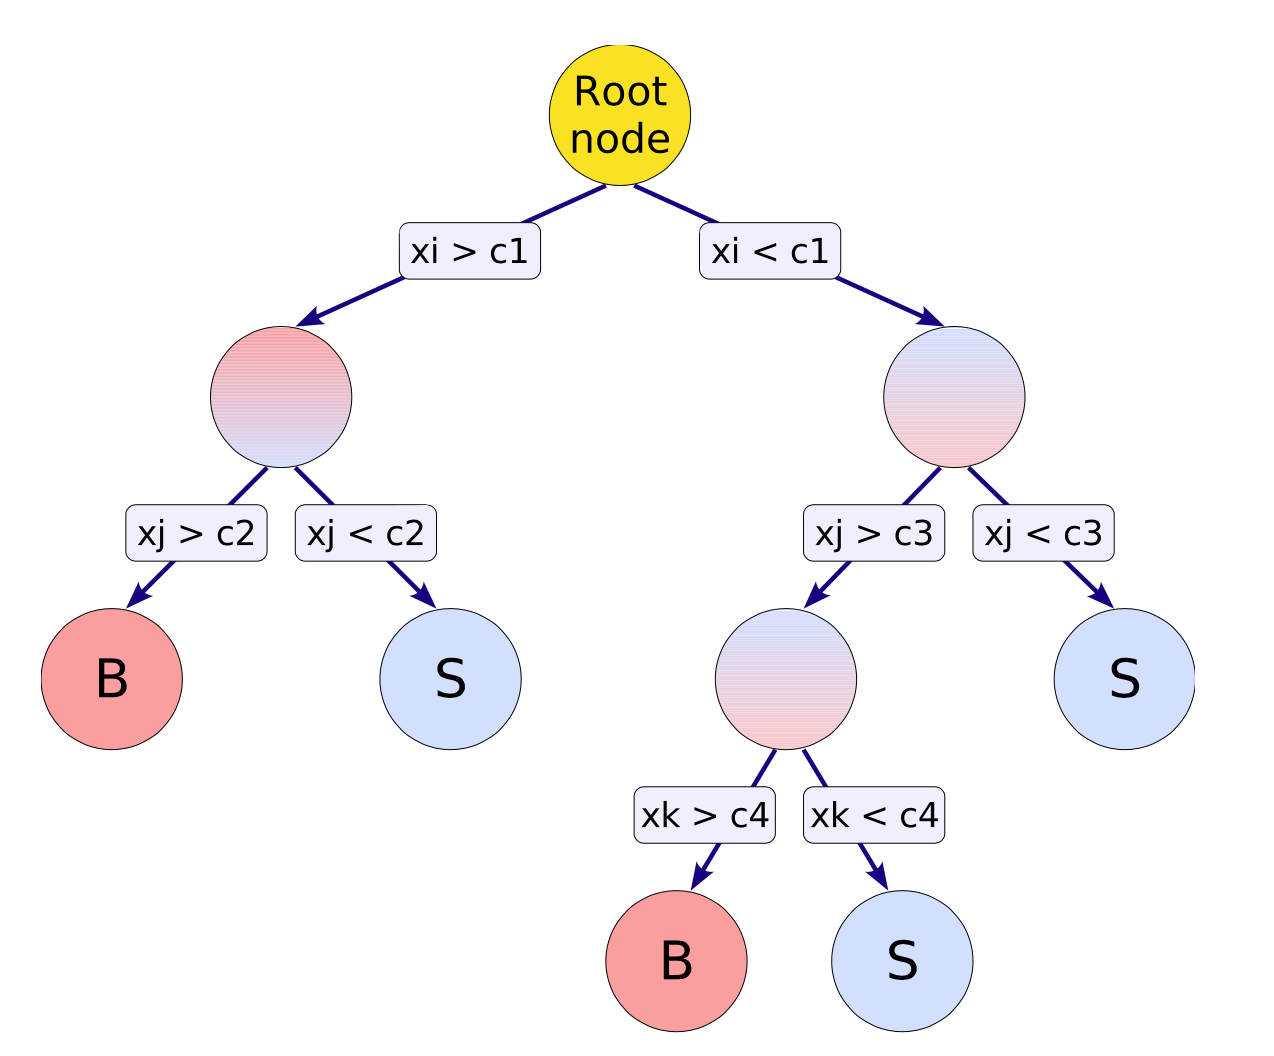
\includegraphics[width=0.5\linewidth]{3_Analysis_techniques/Figures/BDT}
	\caption{Schematic view of a decision tree. Figure taken from \cite{2007physics3039H}.}
	\label{fig:BDTexample}
\end{figure}

 Different trees can be combined into a forest where the final output is determined by the majority vote of all trees, forming the sum of so-called weak learners into one strong learner.   From one training collection, trees are derived by reweighting events, and combined into a single classifier as the  weighted average of each individual decision tree. A method for  making such forests is  boosting a tree. In this method, misclassified events are weighted higher so that future learner concentrate on these events. This has as advantage that the response of the decision trees are stabilised against fluctuations in the training sample which enhances the performance. Additionally, the trees can be kept very shallow, in this thesis i = 3, which improves the robustness against overtraining. Examples of such boosting algorithms are Adaptive Boosting (AdaBoost) and Gradient Boosting~\cite{2014arXiv1403.1452M}. In AdaBoost, each weight of the misclassified events are enhanced while reducing the weight of correctly classified events after each training such that  future events learn those better
\begin{equation}
 \alpha_{\mathrm{n+1}} = \left(\frac{1-\epsilon_{\mathrm{n}}}{\epsilon_{\mathrm{n}}}\right)^{\beta}, 
\end{equation}
where $\epsilon_{\mathrm{n}}$ denotes the misclassification error of the current tree n and $\beta$ is a learning rate. The weight $w_{\mathrm{i}}$ at node i is then equal to $w_{\mathrm{i}} = \mathrm{ln}\:\alpha_{\mathrm{i}}$. The final weight is the sum of all classifiers weighted by their errors. The learning rate is typically chosen to be $\beta\leqslant 0.5$ to allow more boosting steps. Gradient boosting has a similar approach and combines a gradient descent with boosting. Instead of fitting the base-learner to the reweighted data as in AdaBoost, it is fitted to the negative gradient vector of the loss function evaluated at the previous node. Misclassified events will result in a majority vote with large gradients of the loss function. Also for the Gradient boost, the learning rate is typically slow, this also known as shrinkage. In this thesis Gradient boost is used with a shrinkage of 0.2-0.3.
%http://www.ccs.neu.edu/home/vip/teach/MLcourse/4_boosting/slides/gradient_boosting.pdf
%https://indico.scc.kit.edu/indico/event/48/session/4/contribution/35/material/slides/0.pdf
%https://arxiv.org/pdf/1403.1452.pdf
%https://www.quora.com/What-is-the-difference-between-gradient-boosting-and-adaboost
% https://people.phys.ethz.ch/~pheno/Lectures2012_StatisticalTools/slides/Chanon2.pdf

In this thesis, the Gradient boost is used in combination with bagging, so-called stochastic gradient boosting. Bagging is a resampling technique draws a subset of events is  from the training data where the same event is allowed to be randomly picked several times from the parent sample. The tree is then trained on this subset and this is repeated many times. It is based on the assumption that sampling from a dataset that follows a distribution is the same as sampling from the distribution itself~\cite{Behnke:2013:DAH:2564838}. If one draws an event out of the parent sample, it is more likely to draw an event out of the phase space that has a high probability density, as the original dataset will have more events in the regions. Since the selected event is kept in the original sample, the parent sample stays unchanged so that randomly extracted samples have the same parent distribution, albeit statistically fluctuated.  Bagging smears over the statistical fluctuations in the training data, making it suitable for stabilising the response of the classifier and increasing the performance by eliminating overtraining.  In stochastic gradient boosting the bagging resampling procedure uses random sub-samples of the training events for growing the trees. 


The discriminating power of a BDT is assessed by analysing the receiver operating statistics (ROC) curve. This curves show the background rejection over the signal efficiency of the remaining sample. By looking at the area under the curve with respect to random guessing (AUC), the best classifier can be identified. This follows the Neyman-Pearson lemma that the best ROC curve is given by the likelihood ratio \like(x|Signal)/\like(x|Background)~\cite{Behnke:2013:DAH:2564838}. No discrimination power will result in an AUC of 0\%, while 50\%  means fully separated event classes. In \fig{fig:ROC} an example of ROC curve is shown. 
\begin{figure}[htbp]
	\centering
	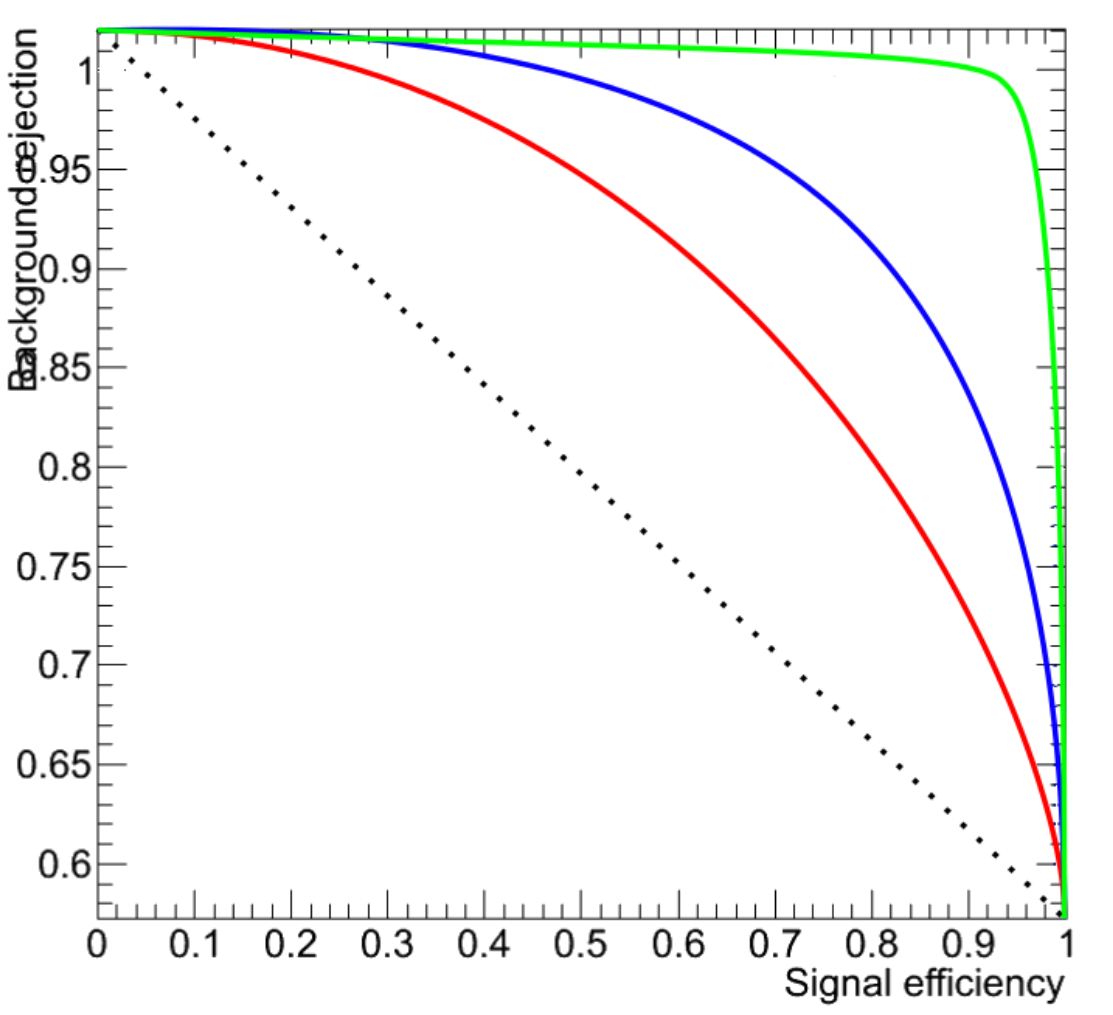
\includegraphics[width=0.5\linewidth]{3_Analysis_techniques/Figures/ROC}
	\caption{Example of ROC curves. In this example, the green method is better than the red one, which is better than the blue one. The dashed line represents a case where there is no separation. Figure taken from \cite{ROC}.}
	\label{fig:ROC}
\end{figure}




\section{Statistical methodology}
\label{sec:Stat}
The search performed in the framework of this thesis requires the simultaneous analysis of data from different decay channels. The statistical methodology used for this search is developped by the ATLAS and CMS collaborations in the context of the LHC Higgs Combination group. The description of the methodology can be found in Refs.~\cite{Chatrchyan:2012tx,Cowan:2010js,CMS-PAS-HIG-12-020,CMS-NOTE-2011-005}. The \texttt{Higgs Combined Tool}~\cite{HiggsCombine} is a 
\texttt{RooStats}~\cite{Moneta:2010pm} framework which runs different statistical methods. In this section, only the statistical tools necessary for the performed search are described. The results presented in this thesis are obtained using the asymptotic formulae~\cite{CLs}.

In general the event yields of signal and background processes are denoted as $s$ and $b$ respectively. These represent event counts in multiple bins or for unbinned probability density functions . By use of simulation, predictions on both signal and background yields are made. These predictions are subject to multiple uncertainties that are accounted for by introducing nuisance parameters $\theta$ such that $s = s(\theta)$ and $b=b(\theta)$. In the following, the actual observed events are denoted as data or observation.

\subsection{The absence of signal: limits}
The absence of a signal is characterised in high energy physics by the Bayesian and modified classical frequentist statistical approaches. They allow to quantify the level of incompatibility of data with a signal hypothesis is terms of confidence  levels (CL). The convention is to require a 95\% CL for excluding a signal. 

An analysis targeting a certain signal production mechanism can either set approximate model-independent limits on signal cross sections times branching ratio ($\sigma \times \BR$) or on the signal cross section times branching ratio times detector acceptance ($\sigma \times \BR \times \accept$). In order to test various theories, the latter is not useful unless the acceptance \accept\ is provided. However, many analysis are not able to present result in a from of limits  on $\sigma \times \BR (\times \accept)$, therefore an alternative is adopted to set limits in the signal strength modifier $\mu$. The signal strength modifier is defined to equally change all the cross sections of all production mechanisms of the signal by the same scale.  sections. 


In this thesis, the modified frequentist approach confidence levels are used~\cite{JUNK1999435,0954-3899-28-10-313}. The classical frequentist  uses a test statistic $q_{\mu}$ based on the profile likelihood ratio to determine how signal- or background-like the data is. However, it does not allow nuisance parameters and is modified to incorporate these.
First a likelihood $\like(\mathrm{data}|\:\mu,\theta)$ is constructed as
\begin{equation}
 \like(\mathrm{data}|\:\mu,\theta) = \mathrm{Poisson}(\mathrm{data}|\:\mu s(\theta)+b(\theta)) \; p(\tilde{\theta}|\theta).
 \label{eq:like}
\end{equation}
The probability density function (pdf) $p(\tilde{\theta}|\theta)$ describes all sources of uncertainty and is described in \Sec{sec:Nuis}. The data in \eq{eq:like} represents either the actual observation or pseudo-data to construct sampling distributions. For a binned likelihood, the Poisson probabilities to observe $n_{\mathrm{i}}$ events in bin i is given as
\begin{equation}
 \mathrm{Poisson}(\mathrm{data}|\:\mu s(\theta)+b(\theta)) = \prod \limits_{\mathrm{i}} \frac{(\mu s_{\mathrm{i}}(\theta) + b_{\mathrm{i}}(\theta))^{n_{\mathrm{i}}}}{n_{\mathrm{i}}!} e^{-\mu s_{\mathrm{i}}(\theta)- b_{\mathrm{i}}(\theta)}.
\end{equation}

At the LHC, the test statistic is defined as 
\begin{equation}
q_{\mu} = -2\: \mathrm{ln} \: \frac{\like(\mathrm{data}|\:\mu, \hat{\theta}_{\mu})}{\like(\mathrm{data}|\:\hat{\mu} , \hat{\theta}_{\mu})}, 
\end{equation}
where the likelihood is maximised in the numerator for a given $\mu$ and (pseudo) data at $\hat{\theta}_{\mu}$, while $\hat{\mu}$ combined with $\hat{\theta}$ defines the point for which the likelihood reaches its global maximum. The estimated signal strength modifier $\hat{\mu}$ can not become negative since a signal rate is positive defined by physics. Furthermore, an upper constraint $\hat{\mu} \leq \mu$ is imposed to guarantee a one sided confidence interval. This has as consequence that upward fluctuations of the data ($\hat{\mu}>\mu$) are not considered against the signal hypothesis\footnote{The signal hypothesis is data with a signal with strength $\mu$.}.  %Note that this definition of the test statistic differs from what has been used at LEP (where “profiling” of systematic errors was not used) and at Tevatron (where systematic errors were profiled, but μ in the denominator was fixed at zero). See Appendix A for details. CMS AN -2011/298

The criterion for excluding the signal at $1-\alpha$ confidence level is the ratio of the probabilities to observe a value of the test statistic at least as large as the one observed in data $q_{\mu}^{\mathrm{obs}}$, under the signal plus background ($s+b$) and background only ($b$) hypothesis is defined as
\begin{equation}
\mathrm{CL} = \frac{\mathrm{P}\left(q_{\mu} \geq q_{\mu}^{\mathrm{obs}}|\: \mu s + b\right)}{\mathrm{P}\left(q_{\mu} \geq q_{\mu}^{\mathrm{obs}}| \:b\right)} \leq \alpha.
\end{equation}
These probabilities are defined as 
\begin{equation}
\begin{aligned}
  p_{\mu} &= \mathrm{P}\left(q_{\mu} \geq q_{\mu}^{\mathrm{obs}}|\: \mu s + b\right) = \int \limits_{q^{\mathrm{obs}}_{\mu}}^{\infty} f(q_{\mu}|\: \mu, \hat{\theta_{\mu}^{\mathrm{obs}}}) \:dq_{\mu}, \\
  1-p_{b} &= \mathrm{P}\left(q_{\mu} \geq q_{\mu}^{\mathrm{obs}}|\:  b\right) = \int \limits_{q^{\mathrm{obs}}_{\mu=0}}^{\infty} f(q_{\mu}|\: \mu=0, \hat{\theta_{\mu=0}^{\mathrm{obs}}}) \:dq_{\mu}, 
\end{aligned}
\end{equation}
where $ p_{\mu}$ and $ p_{b}$ are called the p-values associated to the two hypothesis, and  $f(q_{\mu}|\: \mu, \hat{\theta_{\mu}^{\mathrm{obs}}})$ and $f(q_{\mu}|\: \mu=0, \hat{\theta_{\mu=0}^{\mathrm{obs}}})$ are the pdfs of the signal plus background and background only hypothesis constructed from toy Monte Carlo pseudo data. These pdfs are shown in \fig{fig:pdf}
and are generated with nuisance parameters fixed to $\hat{\theta}_{\mu=0}^{\mathrm{obs}}$ and $\hat{\theta}_{\mu}^{\mathrm{obs}}$.
These values of the nuisance parameters for the background only $\hat{\theta}_{\mu=0}^{\mathrm{obs}}$ and signal plus background  $\hat{\theta}_{\mu}^{\mathrm{obs}}$ hypothesis that best describe the data are found by maximising the likelihood from \eq{eq:like}. The 95\% CL level upper limit on $\mu$ is achieved by adjusting $\mu$ until CL$ = 0.05$
\begin{figure}[htbp]
	\centering
	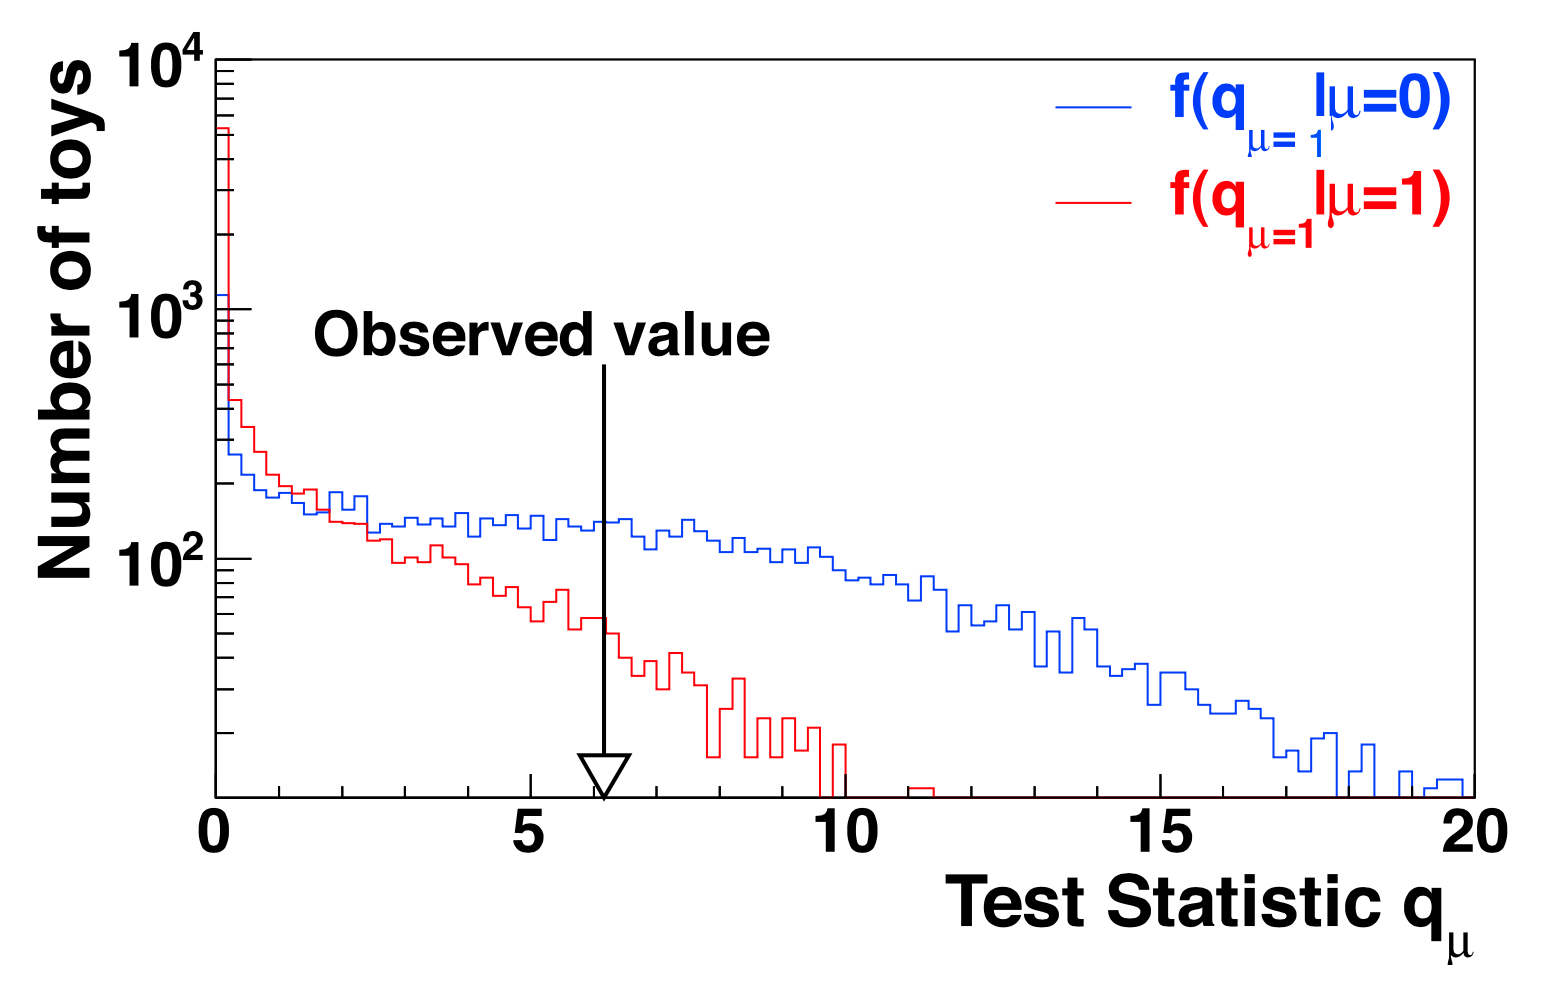
\includegraphics[width=0.7\linewidth]{3_Analysis_techniques/Figures/teststat}
	\caption{Test statistic distributions for pseudo data generated for the signal plus background ($\mu=1$) and background only ($\mu=0$) hypothesis. Figure taken from \cite{CMS-NOTE-2011-005}.}
	\label{fig:pdf}
\end{figure}
\begin{comment}
	Note,
that for the purposes of generating a pseudo-dataset, the nuisance parameters are
fixed to the values θˆobs or θˆobs obtained by fitting the observed data, but are allowed μ0
to float in fits needed to evaluate the test statistic. This way, in which the nuisance parameters are fixed to their maximum likelihood estimates, has good coverage properties [12].
Note that we define pb as pb = P ( q ̃μ < q ̃μ | background-only), excluding the point q ̃μ = q ̃μ . With
these definitions one can identify pμ with CLs+b and pb with 1 − CLb.

If, for μ = 1, CLs ≤ α, we would state that the SM Higgs boson is excluded with (1 − α) CLs confidence level (C.L.). It is known that the CLs method gives conservative limits, i.e. the actual confidence level is higher than (1 − α). See Appendix A for more details.

\end{comment}

The expected median upper limit and the $\pm 1\sigma$ and $\pm 2 \sigma$ bands for a hypothesis is generated by a large set of pseudo data and calculate the CLs and the value of $\mu$ at 95\% CL for each of them. A cumulative probability distribution can be build by starting the integration from the side corresponding to low event yields. The median expected value is where the cumulative distribution function crosses the 50\% quantile. The $\pm 1 \sigma$ (68\%)  and $\pm 2\sigma$ (95\%) bands are defined by the crossings of the 16\% and 84\%, and 2.5\% and 97.5\% quantiles.
\begin{comment}
	Despite being logically very straightforward, this prescription is not too practical from
126 the computational point of view due to the high CPU demand. If N is the number of
127 “toys” being generated in the internal loop of calculations of the desired quantity and
128 M is a number of pseudo-data sets for which such computation is performed, then the
129 number of times the likelihoods would have to be evaluated in such a linear procedure is
130 N·M.
131 To save on the CPU consumption, we use the fact that the distributions of the test
132 statistic for a given μ do not depend on the pseudo-data, so they can be computed only
133 once. The computation of the p-values for each pseudo-data then requires the test statistic
134 to be evaluated only once for each trial value of μ, and the total number of evaluations is
135 proportionaltoN+MinsteadofN·M.
\end{comment}
\subsubsection{Adding sources of uncertainty}
\label{sec:Nuis}
\subsection{Extracting the signal model parameters}
From a scan of the profile likelihood ratio, 
\begin{equation}
q(a) = -2\: \mathrm{ln} \: \frac{\like(\mathrm{obs}|\:s(a) + b, \hat{\theta}_{a})}{\like(\mathrm{obs}|\:s(\hat{a})  + b, \hat{\theta})}, 
\end{equation}
the signal model parameters are evaluated.  The likelihood is maximised by the parameters $\hat{a}$ and $\hat{\theta}$. The likelihood 
\begin{equation}
 \like_{\mathrm{max}} = \like(\mathrm{obs}|\:s(\hat{a}) + b, \hat{\theta})
\end{equation}
is called the best-fit set. 

The 68\% and 95\% CL on a given parameter of interest $a_{\mathrm{i}}$ is then evaluated from $q(a_{\mathrm{i}}) = 1$ or $q(a_{\mathrm{i}}) = 3.84$ respectively, where all other unconstrained model parameters are treated in the same way as the nuisance parameters~\cite{CMS-PAS-HIG-12-020}. 



%http://cds.cern.ch/record/1460438/files/HIG-12-020-pas.pdf
%\subsection{Confidence levels }

%https://indico.cern.ch/event/614672/timetable/#20170907


%
\begin{fmffile}{singletopleptonic}
		\begin{fmfgraph*}(160,40) % width - height
\fmfleft{i1,i2} 
\fmfright{o1,o2,o3,o4,o5}
 \fmf{fermion}{i1,v1,v2,v3,v4,o2}
  \fmf{boson,label=\PZ, label.dist=10}{v2,v6}
  \fmf{fermion}{o4,v6,o3}
   \fmf{gluon}{i2,v1}
   
   \fmflabel{\Pgluon}{i2}
   \fmflabel{\Pup,\Pcharm}{i1}
   \fmffreeze
   \fmf{boson}{v4,v5}
   	\fmfv{label= ,decor.shape=circle,decor.filled=shaded,decor,size=0.5thick, label.angle=-90}{v2}
  % \fmflabel{\Pup,\Pcharm}{i1}
   \fmflabel{\Plepton}{o4}
   \fmflabel{\APlepton}{o5}
   \fmflabel{\Pbottom}{o3}
   \fmflabel{\PW}{o1}
    \fmf{fermion,label=\Pup,,\Pcharm,label.dist=10}{v1,v2}
      \end{fmfgraph*}
\end{fmffile}

%
%	\begin{fmffile}{toppairglugluleptonic}
%	\begin{fmfgraph*}(160,40) % width - height
%		\fmfleft{i1,i2} 
%		\fmfright{o1,o2,o3,o4}
%		\fmflabel{\Pgluon}{i1}
%		\fmflabel{\Pgluon}{i2}
%		\fmflabel{\APup,\APcharm}{o1}
%		\fmflabel{\PZ}{o2}
%		\fmflabel{\PWp}{o3}
%		\fmflabel{\Pbottom}{o4}
%		\fmf{gluon}{i1,v1,i2}
%		\fmf{gluon,label=\Pgluon,label.dist=10}{v1,v2}
%		\fmf{fermion}{o1,v4,v2,v3,o4}
%		\fmffreeze
%		\fmf{boson}{v3,o3}
%		\fmf{boson}{v4,o2}
%		\fmfv{label= ,decor.shape=circle,decor.filled=shaded,decor,size=0.2thick, label.angle=-90}{v4}
%		 \fmf{fermion,label=\Ptop,label.dist=5}{v2,v3}
%		 \fmf{fermion,label=\APtop,label.dist=-20}{v4,v2}
%		\fmflabel{}{v3}
%		\fmflabel{}{v2}
%		\fmflabel{}{v1}
%	\end{fmfgraph*}
%\end{fmffile}


\chapter{Event reconstruction and identification}
\label{chap:4}
The simulated data after the detector simulation described in \Sec{sec:eventgeneration}, has the exact same format as the real collision data recorded at the CMS experiment. Therefore the same software can be used for the reconstruction of both simulation and real data. In \Sec{sec:reco}, the object reconstruction is explained. After reconstructing the objects, they are connected to physics objects, which need to be identified (\Sec{sec:PF}) and corrected for pileup (\Sec{sec:pileup}). The objects used for physics analysis have extra requirements as shown in \Sec{sec:PhysicsObject}. A summary of all the corrections applied to data and simulation is given in \Sec{sec:SummaryCor}.

\section{Object Reconstruction}
\label{sec:reco}
In \fig{fig:transversecms}, the particle interaction in a transverse slice of the CMS detector is shown. When a particle enters the detector, it first enters the tracker where charged particle trajectories, so-called tracks, and origins, so-called vertices, are reconstructed from signals or hits in the sensitive layers. The  magnetic field bends the charged particles making it able to measure the electric charges and momenta of charged particles. The electrons and photons are absorbed in the ECAL and the corresponding electromagnetic showers are detected as clusters of energy in adjacent cells. From this, the energy and the direction of the particles can be determined. The charged and neutral hadrons can also initiate a hadronic shower in the ECAL that is fully absorbed in the HCAL. The clusters from these showers are also used to estimate the energy and direction. Muons and neutrinos pass through the calorimeters without little to no energy loss and the neutrinos even escape the CMS detector undetected while muons produce hits in the muon detectors. 
\begin{landscape}
\begin{figure}
	\centering
	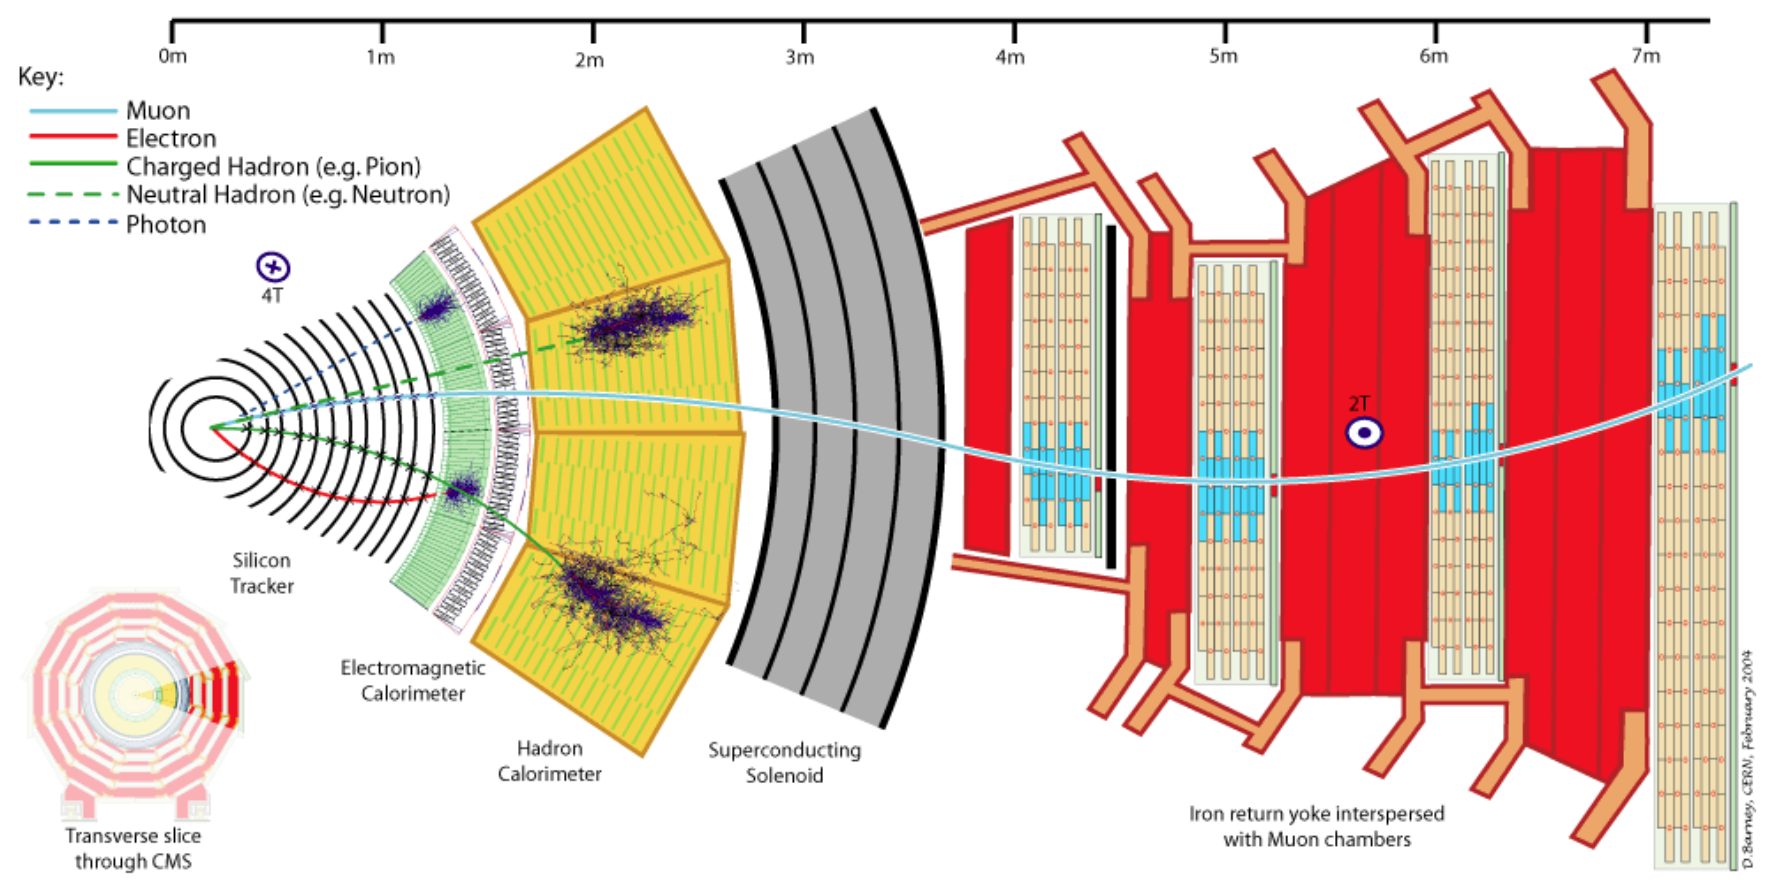
\includegraphics[width=1.\linewidth]{4_EventRecoSelect/Figures/transversecms}
	\caption{Cross-section of the CMS detector with all parts of the detector labelled. This sketch shows the specific particle interactions from a beam interaction reign to the muon detector. The muon and charged pion are positively charged, the electron is negatively charged. Figure taken from~\cite{CMS-PRF-14-001}. }
	\label{fig:transversecms}
\end{figure}
\end{landscape}
%The traditional hadron colliders reconstruction is as follows. The reconstruction of isolated photons and electrons is primarily done by the ECAL, while the identification of muons is based on the muon detectors. Hadrons and photons form jets which are measured by the calorimeters without any contribution from the tracker or muon detectors. Jets can be tagged using the tracker as coming from hadronic \Ptau\ decays or \Pbottom\ hadronisation based on the properties of the relevant charged particle tracks. The missing transverse energy \ptmisvec\ is defined as the vectorial sum of the undetectable particle transverse momenta, and can be reconstructed without any information from the tracker. 
The particle flow (PF)~\cite{CMS-PRF-14-001} reconstruction algorithm correlates the tracks and clusters from all detector layers with the identification of each final state particle, and combines the corresponding measurements to reconstruct the properties. The muon is identified by a track in the inner tracker, connected to a track in the muon detector as described in \Sec{sec:MuonTrack}. The electrons are identified by a track and an ECAL cluster, not connected to an HCAL cluster as described in \Sec{sec:ElectronTrack}. The ECAL and HCAL clusters without a track link identify the photons and neutral hadrons, while the addition of the tracker determines the energy and direction of a charged hadron. \todo{Ik kan hier stoppen en 4.1.1, 4.1.2, 4.1.3.4.1.4 volledig schrappen ( dus enkel primary vertex houden)}


%Coarse-grained detectors can cause signals of different particles to merge and reduce the ability of identifying and reconstructing the particles. Therefore, particle flow identification requires sufficiently segmented subdetectors such that a global event description is possible. The CMS detector is built to meet to requirements of the particle flow reconstruction. It has an efficient and pure muon identification system, a hermetic HCAL with coarse segmentation, a higher segmented ECAL, a fine-grained tracker and a large magnetic field to separate the calorimeter deposits of charged and neutral particles in jets. 

%http://slideplayer.com/slide/2779564/
%http://slideplayer.com/slide/4496166/
\subsection{Charged particle tracks}
An iterative tracking algorithm is responsible for the reconstruction of the tracks made by charged particles in the inner tracking system. Each iteration consists of four steps~\cite{Bayatian:922757}: the track-seed generation, the pattern recognition algorithm, removal of track-hit ambiguities and a final track fit. The pattern recognitions done by use the Kalman filter method~\cite{FRUHWIRTH1987444,Billoir:1989mh} which takes into account the magnetic field and multiple scattering effects. All hits that are unambiguously associated to the final track are removed from the list of available hits. In order to associate the remaining hits, the procedure is repeated with looser track reconstruction criteria. The use of the iterative track reconstruction procedure has a high track finding efficiency, where the fake track reconstruction rate is negligible. 
%For muons, this results in a global track reconstruction efficiency exceeding 98\%, and 75-98\% for charged hadrons. 

\subsection{Following the Muon's Footsteps}
\label{sec:MuonTrack}
% see http://www.bo.infn.it/sminiato/sm16/03_Mercoledi/Mattina/01_Battilana.pdf
% see https://arxiv.org/pdf/1510.05424.pdf
% see https://twiki.cern.ch/twiki/bin/view/CMSPublic/MuonDPGPublic160729
The muon reconstruction~\cite{Chatrchyan:2012xi} has three subdivisions: local reconstruction, regional reconstruction and global reconstruction. The local reconstruction is performed on individual detector elements such as strip and pixel hits in the inner tracking system, and muon hits and/or segments in the muon chambers. Independent tracks are reconstructed in the inner tracker - called tracker tracks -  and in the muon system, called standalone muon tracks. Based on these tracks, two reconstructions are considered: Global Muon reconstruction and Tracker Muon reconstruction. The first is an outside-in approach starting from a standalone muon track while the second uses an inside-out approach starting from tracker tracks. For low transverse momenta ($\pt \lesssim$ 5~\GeV), the tracker muon reconstruction is  more efficient than the global muon approach. This is due to the fact that tracker muons only require a single muon  segment in muon system, while the global muon approach requires typically segments in at least two muon stations. These tracker muons are used for identifying muons from the hadronisation of \Pbottom\ or \Pcharm\  quarks. The global muon approach typically improves the tracker reconstruction for $\pt\gtrsim$ 200~\GeV. %These are labelled isolated when in a cone of $\Delta R = \sqrt{\Delta\phi^2 + \Delta \eta^2} = 0.3$ around the muon, the sum of the transverse momenta of additional tracker tracks and energy deposits in the calorimeter is less than 10\% of the muon's transverse momentum.

%The outside-in approach is referred to as Global Muon reconstruction. 
%For each standalone muon track, a inner tracker track is found by comparing the parameters of the two tracks propagated onto a common surface. Combining the hits from the tracker track and the standalone track, gives a fit via the Kalman filter technique~\cite{FRUHWIRTH1987444,Billoir:1989mh} for a global muon track. 
%
%The second approach is an inside-out reconstruction, creating tracker muons. 
%All candidate tracker tracks with a \pt$>0.5$ \GeV\ and total momentum p$>2.5$ \GeV\ are extrapolated to the muon system taking into account the magnetic field, the average expected energy losses, and multiple Coulomb scattering in the detector material. The extrapolated track and the muon segments are considered matched when the difference in the position in the x coordinates is smaller than 3~\cm, or when the ratio of this distance to its uncertainty is smaller than four. When at least one muon segment - DT or CSC hits -  matches the extrapolated track, the corresponding tracker track is indicated as a tracker muon. 


\subsection{The path of the Electron}
\label{sec:ElectronTrack}
% see also https://arxiv.org/pdf/physics/0512097.pdf
% https://cds.cern.ch/record/1563583/files/ATL-PHYS-PROC-2013-206.pdf
% http://cds.cern.ch/record/1704291
 Standard tracking algorithms are based on Kalman filtering which assume that the energy loss is Gaussian distributed. Since the  electron tracks are increasingly curved in the magnetic field as a function of its flight distance, these standard tracking algorithms are not suitable to fit the electron tracks and different filtering algorithm. The Gaussian sum filter (GSF)~\cite{0954-3899-31-9-N01} is used instead. 

In CMS, the electrons are reconstructed in two ways. The older ECAL based tracking is developed to identify high energetic isolated electrons. This tracking algorithm starts from ECAL clusters with a transverse energy above 4~\GeV\ and extrapolates from these cluster the position of the hits in the tracker. Another, tracker based algorithm uses all the tracks with a \pt\ higher than 2~\GeV\ found with iterative tracking as seeds. The electron seeds from the ECAL- and tracker-based procedures are merged into a unique collection and are then refitted  by using the summed Gaussian distributions as uncertainty per hit in the track fit. The electron efficiency is measured in 8~\TeV\ proton collision data to be better than 93\% for electrons with an ECAL supercluster energy of $E_{\mathrm{T}}>20$~\GeV~\cite{1748-0221-10-06-P06005}. For electrons with an  $E_{\mathrm{T}}>25$~\GeV\  in 13~\TeV\ proton collision data, the efficiency is about 96\%\cite{CMS-DP-2017-004}.


%This tracker algorthm has two main downsides that it is prone to extrapolating a wring position in the tracker and will miss energy deposits
%
%
%In order to account for bremsstrahlung, neighbouring clusters in $\eta$ and $\phi$
%are grouped together into a supercluster from which then the direction is determined to find the position of the particles in the tracker. This has as consequence that for electrons or positrons in jets, energy deposits of surrounding particles will be entering the supercluster leading to a wrong position of the electron/positron in the tracker. Another disadvantage of the ECAL based tracking is that for low \pt\ electrons, the trajectories will be very curved and the supercluster will not contain all of the energy deposit, leading to a higher misconstruction rate. 
%
%The faults of the ECAL based tracking are lifted by adding a tracker based algorithm. This algorithm uses all the tracks with a \pt\ higher than 2~\GeV\ found with iterative tracking as seeds. Iterative tracking uses the Kalman Filter algorithm several times with an average track reconstruction efficiency but high purity. In contrary with a global combinatorial fit, the iterative tracking accepts tracks with a small transverse momentum that are not leaving any energy in the ECAL, and tracks from particles that only interact with the inner tracker layers. When the electron or positron radiated a small amount of energy, the corresponding track can be reconstructed across the whole tracker and safely propagated to the ECAL surface. When there is a larger amount of energy radiated however, the pattern recognition might fail  to accommodate for the change in the electron momentum leading to a track reconstructed with a small number of hits. The solution for this is a preselection based on the $\chi^2$ and number of hits and the selected tracks are fitted again with Gaussian-Sum-Filter which can accommodate substantial energy losses across the trajectory. 



%Due to the lack of coverage of the two pixel discs in high \abspsrap range, the efficiency drops. 
%The resolution on the transverse momentum for a 100 \si{ \GeV} charged particle is about 2.0\% (FIX ME). 
% see https://twiki.cern.ch/twiki/bin/view/CMSPublic/TrackingPOGPlots2016
\subsection{Primary Vertex Reconstruction}
The primary vertex (PV) reconstruction is able to measure the location of all proton interaction vertices in each event consisting of the signal vertex and all vertices from pileup events. First, tracks are selected  to be consistent with being produced promptly in the primary interaction~\cite{Chatrchyan:1704291}. Then the tracks are grouped according to the $z$ coordinate of their closest approach to the beam line~\cite{726788} and a vertex fitting algorithm~\cite{Waltenberger:1166320} is performed. The primary vertex is found as the vertex corresponding to the highest sum of squared track transverse momenta and is taken to be the main interaction point. The resolution on the primary vertex is about 14 \si{ \micro \meter} in $r\phi$ and about 19 \si{ \micro \meter} in the $z$ direction for primary vertices with the sum of the track $p_T > 100$ \si{ \GeV} for 2016 data taking.
% numbers from https://twiki.cern.ch/twiki/bin/view/CMSPublic/TrackingPOGPlotsICHEP2016

\subsection{Calorimeter clusters}
The energy and direction of stable neutral particles such as photons and neutral hadron are reconstructed using a cluster algorithm.  This algorithm also separates neutral particles from charged hadron energy deposits, 
and reconstructs and identifies electrons and their bremsstrahlung photons. Furthermore, the cluster algorithm is contributing to the energy measurements of charged hadrons that don't have accurate tracks parameters, e.g. for low quality and high transverse momentum tracks. The clustering is performed separately in each subdetetector: ECAL barrel and endcaps, HCAL barrel and endcaps, and the two preshower layers. The HF has no clustering algorithm since the electromagnetic or hadronic components give rise to an HF EM or HF HAD cluster. 

The clustering algorithm consist of different steps. First seeds are identified when cells have an energy larger than the seeding threshold and larger than their neighbouring cells. Then topological clusters are made by accumulating cells that share at least a corner with a cell already in the cluster and an energy above a cell threshold set to twice the noise level. The third step is an expectation maximization algorithm that reconstructs the cluster~\cite{CMS-PRF-14-001} and assumes that  the energy deposits are Gaussian distributed. The calorimeter clusters are used for reconstructing photons and neutral hadrons. The  clusters that are not in the vicinity of the extrapolated charged tracks are identified as neutral hadrons or photons. If the energy deposits are in vicinity of charged tracks, such is the case for charged hadrons, the neutral particle energy deposit is measured as an excess over the charged particle deposit. %For this reason, a good calibration of the electromagnetic and hadronic calorimeter is  vital. 

%The ECAL calibration is performed before the hadron cluster calibration or particle identification. For run 1, the ECAL response to electrons and photons as well as the cell-to-cell relative calibration is determined with test beam data, radio active sources, and cosmic ray measurements. For run 2, the collision data collected at 7 and 8~\TeV\ was used to refine the calibration. The effect of the thresholds in the clustering algorithm are estimated from simulated single photons with energies varying from 0.25 to 100~\GeV. The photons used for the calibration should not have a conversion prior to their entrance to ensure the calibration of single clusters. In all ECAL regions and for all energies, the calibrated photon energies agree with the true photon energies within 1\%.
%
%In contrary to the photons, the hadrons deposit in general energy in both ECAL and HCAL. Since the calorimeter response in the HCAL depends on the fraction of shower energy deposited in the ECAL, the ECAL and HCAL cluster energies are recalibrated together to get an estimate of the true hadron energy. Since the calibration is done for hadrons, single neutral hadrons such as $K_{\mathrm{L}}^0$ are used for determining the calibration constants. The hadrons interaction with the tracker material are rejected for the calibration purposes. This calibration is checked with isolated charged hadron selected from early data recorded at $\sqrt{s}=0.9, 2.2$ and 7 \TeV.  

%\section{Putting the pieces together}


%The link between a central tracker track and a calorimeter clusters is made by extrapolating the tracker track to the two layers of the preshower, the ECAL, and the HCAL. If this extrapolated position is within the cluster area, the two are linked. When there are several ECAL or HCAL clusters for the same track, the link with the smallest distance is kept. A dedicated cluster algorithm accounts for the energy of the photons emitted through bremsstrahlung at for photons that have converted to an electron-positron pair. \\The ECAL to HCAL cluster and ECAL to preshower cluster links are established when the cluster position in the more granular calorimeter, ECAL or preshower, is in accordance with the cluster envelope of the less granular calorimeter, HCAL or ECAL.  When there are multiple HCAL clusters linked to the same ECAL cluster, the link with the smallest distance is kept. This is also true for multiple ECAL clusters with the same preshower clusters. The ECAL supercluster is linked with the ECAL cluster when they share at least one ECAL cell. \\
%Nuclear interactions in the tracker can lead to kinks in hadron trajectories as well as the production of secondary particles. This leads to charged particle tracks linked together via a common displaced vertex. The displaced vertices considered should have at least three tracks, with at most one incoming track, and the invariant mass of the outgoing tracks should exceed 0.2~\GeV. \\
%The link between a track and the muon detectors is done via local, regional, and global reconstruction as explained in \Sec{sec:MuonTrack}. 


\section{Particle flow identification}
\label{sec:PF}
The several PF elements from the various CMS subdetectors are connected through a link algorithm. This algorithm tests any pair of elements in an event, only considering nearest neighbours in the $\eta\phi$-plane. The quality of the link is determined via the distance between the two elements and PF blocks of elements are formed from elements with a direct link or indirect link through common elements. The identification and reconstruction follows a particular order in each PF block. After each identification and reconstruction the corresponding PF elements (tracks and clusters) are removed from the PF block.

 The muons are the first to be identified and reconstructed. These are reconstructed if their momenta are compatible with corresponding track only momenta. Then the electron and its corresponding brehmstrahung photons, are identified and reconstructed by using of the GSF tracking. At the same time, the energetic and isolated photons are identified as well. The remaining elements in the PF block are subjected to a cross identification of charged hadrons, neutral hadrons, and photons that arise from parton fragmentation, hadronisation, and decays in jets. The charged hadron candidate is made from the remaining candidates that have a charged particle track associated with them. Then the charged particle energy fraction is subtracted from the calibrated energy of the linked calorimeter clusters and the remaining energy is assigned to the neutral energy. Depending on the excess of neutral energy in the ECAL and HCAL clusters, a photon or a neutral hadron is assigned respectively. The pseudorapidity range of the inner tracker limits the information on the particles charge to $|\eta| < 2.4$. Outside this range a simplified identification is done for hadronic and electromagnetic candidates only. 

%\subsection{Muons}
%\label{sec:Muon}
%A set of selection requirements based on the global and tracker muon properties is responsible for muon identification. The muons are considered isolated when the additional inner tracks and calorimeter energy deposits within a distance to the muon direction in the $\eta\phi$-plane is smaller than 0.3. The muons coming from charged hadron decays or heavy flavour decays need more stringent criteria. This due to the fact that charged hadrons can be misidentified as muons because of e.g. punch-through, or muons can be seen as charged hadrons, and will absorb the energy deposits of nearby particles. 
%\subsection{Electrons and isolated photons}
%\label{sec:Electron}
%The electrons and photons are reconstructed together as discussed before. An electron candidate seeded from a GSF track is considered an electron when the linked ECAL cluster is not linked to three or more additional tracks. The photon seeds are ECAL superclusters with transverse energies above 10~\GeV\ that have no links with a GSF track. After associating photons from brehmstrahung with the associated electrons, the remaining energy is associated to the photons and the photon direction is taken to be that of the supercluster. The electron direction is chosen to be that of the GSF track and its energy is a combination of the ECAL energy with the momentum of the GSF track. Photons are retained if they are isolated, while electrons should satisfy additional criteria based on a multivariate analysis for isolated and non-isolated electrons. 
%\subsection{Hadrons and non-isolated photons}
%\label{sec:Hadron}
%After muon, electron and isolated photon identification, the remaining particles are hadrons from jet fragmentation and hadronisation. These can show up as charged hadrons (e.g. $\pi{\pm}$, $\mathrm{K}^{\pm}$, or protons), neutral hadrons (e.g. $\mathrm{K}^{0}_{\mathrm{L}}$ or neutrons), non isolated photons (e.g. from $\pi^0$ decays), and additional muons from early decays of charged hadrons. 
%
%The photons and neutral hadrons are assigned to calorimeter clusters without any link to tracks. When the calorimeter clusters between the ECAL and HCAL are linked, the clusters are assumed to arise from the same hadron shower. If their is not such a link, HCAL clusters are assigned to neutral hadrons, while the ECAL clusters are assigned to photons based on the fact that neutral hadrons leave only 3\% of their energy in the ECAL. The HCAL clusters linked with tracks, that are not linked with other HCAL clusters, are assigned to charged hadrons. These tracks are then linked with remaining ECAL clusters. 
%
%Hadron interactions can result in the creation of extra particles originating from a secondary vertex. These extra particles are identified by having a common secondary vertex and replaced in the PF list as one single primary charged hadron. 
%
%
%\subsection{Post processing}
%\label{sec:Postprocess}
%After identification and reconstruction of all particles as described above. An artificial large missing transverse momentum \ptmisvec\ can be reconstructed. The cause of the \ptmisvec\ is mostly misidentified or misreconstructed high-\pt\ muons originating from cosmic rays, misconstruction of the muon's momentum, or punch-through charged hadrons. A post processing step is applied to solve this \ptmisvec. Events with genuine large \ptmisvec\ due to the presence of neutrino's are unaffected by this post processing.


\section{Pileup mitigation and luminosity measurement}
\label{sec:pileup}
For the 8 \TeV\ dataset, an average of about 21 pileup interactions happen per bunch cross section. For the dataset taken at 13 \TeV, the number of pileup interactions increases to about 27 interactions per bunch crossing.  These interactions are spread around the beam axis around the centre of the CMS coordinate system and follow a normal distribution with a standard deviation of about 5 \cm~\cite{CMS-PRF-14-001}.  The number of pileup interactions is estimated from the number of interaction vertices reconstructed from charged particle tracks, or from the instantaneous luminosity of the given bunch crossing with dedicated detectors and the inelastic proton-proton crossing. The luminosity of the CMS interaction point is estimated from measuring certain process rates with luminometers such as the pixel detector, HF calorimeter, and the pixel luminosity telescope~\cite{Kornmayer:2039978}. The instantaneous luminosity from recorded process rate $R$ is then determined as 
\begin{equation}
\lumi dt = \frac{R dt }{\sigma_{\mathrm{fid}}}, 
\end{equation} 
where $\sigma_{\mathrm{fid}}= \sigma \times A$ corresponds to the fiducial cross  section recorded in the luminometer acceptance $A$ which is determined using van der Meer scans~\cite{CMS-PAS-LUM-17-001}. The overall uncertainty on the luminosity measurement is estimated to be 2.5\%.  

The luminosity is used to infer the number of pileup interactions in data, which can be used to correct the predefined pileup interactions in simulation. Then an event weight can be derived from the ratio of the distributions of pileup interactions in data and simulation. For 13 \TeV\ collisions, the inelastic cross section is measured to be $71.3\pm3.5$ mb~\cite{CMS-PAS-FSQ-15-005}. However a better agreement in data and simulation for the pileup sensitive variables, such as the number of primary vertices, is found with a lower cross section of 69.2 mb with an uncertainty of 4.6\%. %this due to h ehip effect so the data was more inefficient https://hypernews.cern.ch/HyperNews/CMS/get/luminosity/613/2/1/1/1.html

%The pileup vertices are separated from the primary vertex by requiring that the primary vertex is the vertex with the highest quadratic sum of the transverse momenta of the corresponding tracks. The charged hadrons coming from these pileup vertices are identified via their tracks and are removed from the list of reconstructed particles to be used for physics analysis. This method is the so-called pileup charged hadron subtraction and denoted as CHS~\cite{CMS-PAS-JME-14-001}. For the reconstructed particles outside the tracker acceptance as well as photons and neutral hadrons, the CHS method doesn't work. Therefore, the transverse density from pileup interactions is estimated using jet clustering techniques and their effect is subtracted from the particles transverse momenta. Additionally, the pileup contribution can be estimated locally as described for the muons and electrons described in \Sec{sec:MuonID} and \Sec{sec:ElectronID}. 



\section{Physics object reconstruction and identification}
\label{sec:PhysicsObject}
The particle flow objects are used for building physics objects that are used for analysis. Analyses use jets, muons, electrons, photons, taus and missing transverse momentum \ptmisvec with extra, analysis dependent requirements. In the following section, only the physics objects used throughout this thesis are discussed. 

\subsection{Muons}
\label{sec:MuonID}
The muon candidates used for analysis in this thesis correspond to the tight and loose working point. Detailed reports on the performance can be found in~\cite{CMS-DP-2017-007}.

The tight working point rejects objects wrongly reconstructed as muons from hadron showers that reach the muon system (punch-throughs), by requiring that the global muon fit includes at least one valid hit in the muon chambers for which at least two muon segments in two muon stations are present. Furthermore, the muon tracks should have a global fit yielding a goodness-of-fit of $\chi^2 / \mathrm{ndof} < 10$. Requiring at least one pixel hit in the muon track suppresses the decay of muons in flight. Also a minimum of five hits in the tracker is required. Cosmic muons and muons originating from pileup interactions are rejected by constricting the distance of the muon with respect to the primary vertex by putting limits on $d_{\mathrm{x,y}}< 2$ \mm\ and $d_{\mathrm{z}}<5$ \mm. Also muons according to the loose muon working point will be used in the thesis. These are either global muons or tracker muons reconstructed from the particle flow muon object. In \tab{tab:MuonReq}, the muon requirements for the muons used throughout this thesis are summarised.  In \fig{fig:tightid}, the muon efficiencies for data and simulation are presented. These efficiencies are estimated from tag-and-probe methods~\cite{CMS-DP-2017-007}.
% that select $\PZ \rightarrow \Pmuon \APmuon$ and tag one muon that passes the identification criteria. The other muon is used as probe and one measures how many times it passes the identification criteria to get the efficiency. 
Overall, the efficiency is about 95-100\%, with two drops due to the crack between the wheels of the DT system. The differences between data and simulation are corrected by applying \pt- and $\eta$-dependent scale factors ($\epsilon_{\mathrm{data}}/\epsilon_{\mathrm{MC}}$) to simulated events. 
\begin{figure}[htbp]
	\centering
	\includegraphics[width=0.495\linewidth]{4_EventRecoSelect/Figures/TightIDvseta}
	\includegraphics[width=0.495\linewidth]{4_EventRecoSelect/Figures/LooseIDvseta}
	\caption{Comparison of the muon tight ID (left) and loose ID (right) efficiencies in data and simulation as a function of the pseudorapidity of the muon using the full 2016 dataset. Figure taken from \cite{CMS-DP-2017-007}.}
	\label{fig:tightid}
\end{figure}

In addition to the identification criteria, the muons are required to be spatially isolated from electromagnetic and hadronic activity.  The relative lepton isolation is defined as estimating the total transverse energy of the particles emitted around the  direction of the lepton by defining a cone of radius $\Delta R$ in $\eta\phi$ plane around the lepton direction. Then a summed energy is calculated from the charged hadrons (CH), neutral hadrons (NH), and photons (\Pphoton), excluding the lepton itself. This sum is then corrected to remove the energy coming from pileup interactions. The relative isolation for muons $\iso_{\Pmu}$ is defined as~\cite{CMS-PRF-14-001}:
\begin{equation}
 \iso_{\Pmu} = \frac{\sum \pt(\mathrm{CH}) + \mathrm{max}\left(0., \sum \Et(\mathrm{NH}), \sum \Et(\Pphoton) - 0.5 \times \sum \Et (\mathrm{CH})\right)}{\pt(\Pmu)},
\end{equation}
where a cone of $\Delta R = 0.4$ is adopted and the pileup mitigation is based on the  \dbeta\ correction. The \dbeta\ correction estimates the pileup energy as half of the contribution coming from charged hadrons. For tight ID muons, this relative isolation should $\iso_{\Pmu} <0.15$, while for loose muons this should be $\iso_{\Pmu} <0.25$. % The chosen value for β is motivated by assuming equal production rates for the (π+,π0,π−) isospin triplet leading to a ratio of 1/2 for the production of neutral pions over charged ones. 
In \fig{fig:muoniso}, the isolation efficiencies as a function of the pseudo rapidities using the tag and probe method are shown for the tight muon working point. The efficiencies are 85-100\%  and have a decline for low-\pt\ muons. % These low-\pt\ muons are most likely coming from hadronic or heavy flavour decays. 
The differences between data and simulation are accounted for by applying $\eta$- and \pt-dependent scale factors on the simulation. 
\begin{figure}[htbp]
	\centering
	\includegraphics[width=0.494\linewidth]{4_EventRecoSelect/Figures/TightIsovsot}
	\includegraphics[width=0.494\linewidth]{4_EventRecoSelect/Figures/TightIsovseta}
	\caption{Comparison of the muon tight isolation requirement with the muon tight ID  efficiencies in data and simulation as a function of the transverse momentum (left) or  pseudorapidity (right) of the muon using the full 2016 dataset. Figure taken from \cite{CMS-DP-2017-007}.}
	\label{fig:muoniso}
\end{figure}
\begin{table}[htbp]
	\centering
	\caption{Muon requirements for the tight and loose working points, used throughout this thesis.}
	\begin{tabular}{ccc}
		\toprule
		Properties & Loose Muons & Tight Muons \\ 
		\midrule 
		Global muon or Tracker Muon & One or the other & Both \\ 
	
		Particle Flow muon & Y & Y \\ 
		
		$\chi^2/\mathrm{ndof}$ of global muon track fit & N/A & $<$ 10 \\ 
	
		Nb. of hit muon chambers & N/A & $>$ 0 \\ 
		
		Nb. of muon stations contained in the segment & N/A & $>$ 1  \\ 
		
		 Size of the transverse impact parameter  & \multirow{2}{*}{N/A }& \multirow{2}{*}{$d_{xy} < 2$ \mm} \\ 
	 of the track wrt. the PV & & \\
		Longitudinal distance wrt. the PV & N/A & $d_z < 5$ \mm \\ 
		
		Nb. of pixel hits & N/A & $>$ 0 \\ 
		
		Nb. of tracker layers with hits & N/A & $>$ 5 \\ 
	
		Relative Isolation & $<$0.25 & $<$0.15 \\
		\bottomrule
	\end{tabular} 
	
	\label{tab:MuonReq}
\end{table}


\newpage
\subsection{Electrons}
\label{sec:ElectronID}
The electron candidates used, correspond to the tight and veto working points. The study of the electron reconstruction and identification performance can be found in \cite{CMS-DP-2017-004}.

Starting from an electron PF candidate with a GSF track that is outside the barrel-endcap transition region ($1.4443 < |\eta| <1.5660$), several requirements are set. The electron track should not have more than one (two or three) missing hit(s) in the innermost layer for the tight (veto) working point. This dismisses electrons from photon conversions. Additionally, a photon conversion veto is applied by testing if a pair of electron tracks is originating from a common displaced vertex. Furthermore, refined cuts are applied on the shower shape variables such as the difference in $\eta$ or $\phi$ between the energy weighted supercluster position in the ECAL and the track direction  at the innermost tracker position ($\Delta \eta_{\mathrm{in}}$, $\Delta \phi_{\mathrm{in}}$), and the ECAL crystal based shower covariance in the $\eta$ direction ($\sigma_{\eta \eta}$). These cuts also include energy related variables such as the absolute difference between the inverse electron energy measured in the ECAL and the inverse momentum measured in the tracker ($|1/E-1/p|$), and the ratio of the energy measured in the HCAL and ECAL (H/E). Unlike the muon case, the identification criteria also contain requirements on the isolation of the electrons.

Similar to the muons, the electron  relative isolation is determined from the sum of the particles in a cone around the electron itself. The cone radius used for electrons is $\Delta R=0.3$ and a $\rho$ correction for pileup mitigation is applied. For this correction, the expected pileup energy inside the isolation cone is estimated from the median density energy per area of pileup contamination ($\rho$), computed event by event, and the effective area ($A_{\mathrm{eff.}}$)~\cite{CMS-PRF-14-001}. This effective area is estimated from simulation and denotes the expected amount of neutral energy from pileup interactions per $\rho$ within the isolation cone as a function of the pseudo rapidity of the associated ECAL superclusters. Table \ref{tab:EAeff} shows the values used for 13 \TeV\ data. The relative electron isolation $\iso_{\Pe}$  is calculated as
\begin{equation}
\iso_{\Pe} =  \frac{\sum \pt(\mathrm{CH}) + \max\left(0., \sum \Et(\mathrm{NH}), \sum \Et (\gamma) - \rho \times A_{\mathrm{eff.}}\right)}{\pt(\Pe)}.
\label{eq:drho}
\end{equation}
\begin{table}[htbp]
	\centering 
	\caption{The effective areas  $A_{\mathrm{eff.}}$ used for the electron relative isolation~\cite{ilya}.}
	\begin{tabular}{cc}
		\toprule 
		$\eta$ region  & $A_{\mathrm{eff.}}$ \\ 
		\midrule
		$0<|\eta| < 0.1752$ & 0.1703 \\ 
	
		$1.0<|\eta| < 0.1479$ & 0.1715 \\ 
	
		$1.479<|\eta| < 2.0$ & 0.1213 \\ 
	
		$2.0<|\eta| < 2.2$ & 0.1230 \\ 
	 
		$2.2<|\eta| < 2.3$ & 0.1635 \\ 
	
		$2.3<|\eta| < 2.4$ & 0.1937 \\ 
		 
		$2.4<|\eta| < 2.5$ & 0.2393 \\ 
		\bottomrule
	\end{tabular} 
	\label{tab:EAeff}
\end{table}

The efficiency of electron identification is estimated from $\PZ \rightarrow \Pelectron \APelectron$ events via the tag-and-probe method and is shown in \fig{fig:electrontightidvspt} for the tight working point. The efficiencies reach $95-100$\%.  The difference between  data and  simulation is corrected for by dedicated $\pt$- and $\eta$ dependent scale factors as well. 
\begin{figure}[htbp]
	\centering
	\includegraphics[width=0.5\linewidth]{4_EventRecoSelect/Figures/ElectronTightIDvsPt}
	\caption{Electron identification efficiency as function of the electron transverse momentum from the full 2016 dataset. Figure taken from \cite{CMS-DP-2017-004}.}
	\label{fig:electrontightidvspt}
\end{figure}

\begin{table}[htbp]
	\centering
	
	\caption{Electron requirements used in this analysis. The requirements are set in the barrel ($|\eta_{supercluster}| \leq 1.479$)
		and the endcaps ($|\eta_{supercluster}| > 1.479$). }
	\begin{tabular}{ccccc}
		\toprule
		Properties & \multicolumn{2}{c}{$|\eta_{supercluster}| \leq 1.479$ } & \multicolumn{2}{c}{$|\eta_{supercluster}| > 1.479$ } \\
		
		& Veto electron & Tight electron & Veto electron & Tight electron \\ 
	  \midrule
		$ \sigma_{\eta \eta}$ & $<$ 0.0115 & $<$ 0.00998 & $<$ 0.037 & $<$ 0.0292 \\ 
	
		$|\Delta \eta_{\mathrm{in}}|$ & $<$ 0.00749 & $<$ 0.00308 & $<$ 0.00895& $<$ 0.00605\\ 
	 
		$|\Delta \phi_{\mathrm{in}}|$ & $<$ 0.228 & $<$ 0.0816 & $<$ 0.213& $<$ 0.0394 \\ 
		
		H/E & $<$ 0.356 & $<$ 0.0414 & $<$ 0.211& $<$ 0.0641 \\ 
		
		relative isolation & $<$ 0.175 & $<$ 0.0588  & $<$ 0.159& $<$ 0.0571\\ 
	
		$|1/E-1/p|$ & $<$ 0.299 \GeVinv& $<$ 0.0129 \GeVinv& $<$ 0.15 \GeVinv&$<$ 0.0129 \GeVinv\\ 
	
		expected missing inner hits & $\leq $ 2 & $\leq $ 1 &  $\leq $ 3 &  $\leq $ 1\\ 
		%		\hline
		%		d0 - dz & 0.05 cm & 0.05 cm & 0.10 cm & 0.10 cm \\
		
		pass conversion veto & Y & Y & Y & Y\\ 
		\bottomrule
	\end{tabular} 
	\label{tab:ElecReq}
\end{table}


\subsection{Jets}
\label{sec:JetID}
%https://twiki.cern.ch/twiki/bin/view/CMS/IntroToJEC
Jets are reconstructed  from all reconstructed particles without the charged hadrons associated to pileup vertices. The clustering is done via the \antikt\ algorithm~\cite{Cacciari:2008gp} with a radius parameter for the cone size of the resulting jet of $R=0.4$. %The initial step of the \antikt\ algorithm considers all candidates as ''protojets" and starts to calculate the distances for protojets i and j as
%\begin{equation}
%\begin{aligned}
%   d_{\mathrm{ij}} &= \mathrm{min}\left(\frac{1}{p_{\mathrm{T,i}}^2}, \frac{1}{p_{\mathrm{T,j}}^2}\right), \\
%   d_{\mathrm{i}} &= \frac{1}{p_{\mathrm{T,i}}^2}.
% \end{aligned}
%\end{equation}
%For each iteration the two distances are calculated. When $d_{\mathrm{ij}} < d_{\mathrm{i}}$, the two protojets are merged and their four momentum is summed. If $d_{\mathrm{i}}$ is the smallest distance, the protojet is renamed as final jet and ignored in the subsequent steps. 
More information about the jet algorithm performance can be found in Ref. \cite{CMS-PAS-JME-16-003}.

The jets used for the analysis  in this thesis, use the loose identification working point summarised in \tab{tab:jetID}. The requirements on the jet constituents are based on the assumption that a proper jet originating from the hadronisation of a quark or gluon consists of multiple PF particles and types. Therefore, the jet should consists of more than one constituent, and the neutral hadron fraction and neutral EM energy fractions should be less than 99\%. For the jets within the tracker acceptance ($|\eta|<2.4$), at least one constituent has to be a charged hadron resulting in a charged hadron energy fraction above 0\%. Additionally the charged EM energy fraction should be less than 99\%. On top of these requirements, objects that are labelled as jets and found in vicinity of any isolated lepton, $\Delta R < 0.3$, are removed from the jet collection in that event to avoid duplications of objects. 
\begin{table}[h]
	\centering
	\caption{Jet criteria used throughout the thesis. The last three requirements are only for jets within the tracker acceptance.}
	\begin{tabular}{cc}
		\toprule 
		Properties & Loose Jet ID \\ 
		\midrule
		Neutral hadron fraction & $<$ 0.99 \\ 
		
		Neutral EM fraction & $<$ 0.99 \\ 
		
		Number of constituents & $>$ 1 \\ 
		 		
		Charged hadron fraction & $>$ 0 \\ 
	 
		Charged multiplicity & $>$ 0 \\ 
		
		Charged EM fraction & $<$ 0.99 \\ 
		\bottomrule
	\end{tabular} 
	\label{tab:jetID}
\end{table}

The energy of the reconstructed jets deviates from the energies of the corresponding jets clustered from the hadronisation products of true partons from simulations due to non-linear subdetetector response and efficiencies. The jet energy corrections (JEC) calibrate the jets in order to have the correct energy scale and resolution.
Jet energy scale corrections (JES) are determined as a function of pseudorapidity and the transverse momentum from data and simulated events by combining several channels and methods. This is extensively described in \cite{1748-0221-12-02-P02014}. These corrections account for the effects of pileup, the uniformity of the detector response, and residual data-simulation jet energy scale differences. Furthermore, the jet energy resolution (JER) is measured in data and simulation as function of pileup, jet size and jet flavour.  %A detailed understanding of both the energy scale and the transverse momentum resolution of the jets is crucial for many physics analysis, and these are commonly the main source of systematic uncertainty.
 The performance of the jet energy corrections for the 13 \TeV\ dataset can be found in \cite{CMS-DP-2016-020}.


The JEC are factorised and subsequently correct for the off-set energy due to pileup, the detector response to hadrons, and residual differences between data and simulation as a function of the jet pseudorapidity and transverse momentum.  The consecutive steps of JEC are shown in \fig{fig:jes}. 
\begin{figure}[htbp]
	\centering
	\includegraphics[width=1.\linewidth]{4_EventRecoSelect/Figures/JES}
	\caption{The sequence of the JEC for data and simulations The corrections marked with MC are derived from simulation studies, while RC stands for random cone, and MJB for the analysis of multi-jet events. Figure taken from \cite{1748-0221-12-02-P02014}.}
	\label{fig:jes}
\end{figure}
The off-set corrections remove the dependency of the jet energy response of additional pileup activity. It is based on the jet area method, which uses the effective area of the jets multiplied by the average density in the event, to calculate the off-set energy to be subtracted of the jets.  The correction factors are derived by comparing the jet response with and without pileup events overlaid. The residual differences between data and detector simulation are determined using the random cone method (RC). For this method, many jets are reconstructed in each event by clustering particles through placing  random cones. This provides a mapping of the $\eta\phi$-space and the average \pt\ of those jets gives the average energy off-set due to pileup~\cite{1748-0221-12-02-P02014}. 
The next level of corrections have as goal to have a uniform energy response independent of the transverse momentum or pseudorapidity of the jet.  These corrections are determined from simulated events by matching the reconstructed to true particle jets and comparing there momenta. 
The residual corrections between data and simulation are determined by comparing the transverse momentum balance in various types of events (multi-jet, \Zjets, and \pjets), using a reference jet in the barrel region.  
The jet flavour corrections are optional and not used for this thesis. More information on the jet flavour corrections can be found in \cite{1748-0221-12-02-P02014}. For jets with a transverse momentum above 30~\GeV, the uncertainties from the various corrections are 3-5\% for the 13 \TeV\ dataset~\cite{CMS-DP-2016-020}.


After applying JEC, the transverse momentum resolution of the jet is extracted from data and simulated events. There are two methods used to rescale the reconstructed four momentum based on whether or not the simulated jet can be matched to a true jet  in simulation. The factors are defined as
\begin{equation}
\begin{aligned}
c_{\mathrm{matched}} &= 1 + \frac{\pt^{\mathrm{reco.}}-\pt^{\mathrm{true}}}{\pt^{\mathrm{reco.}}} \left(s_{\mathrm{JER}} -1\right), \\
c_{\mathrm{unmatched}} &= 1 + \mathrm{N}(0, \sigma_{\mathrm{JER}})\sqrt{\mathrm{max}\left(s^2_{\mathrm{JER}}-1, 0\right)},
\end{aligned}
\end{equation}
where $ \mathrm{N}(0, \sigma_{\mathrm{JER}})$ denotes a sample value from a normal distribution centred at zero with as standard deviation the relative resolution in simulation $\sigma_{\mathrm{JER}}$, and $s_{\mathrm{JER}}$ the $\eta$-dependent resolution scale factors. These scale factors are derived  from data from di-jet or \pjets\ events and analysing the \pt\ balance. The resolution scale factors (data/simulation) are found to be 1.1-1.2, except for the transition regions around $|\eta| =3$ and $|\eta| = 1.4$~\cite{CMS-DP-2016-020} and given in Table \ref{tab:JER}.
\begin{table}[htbp]
	\centering
	\caption{Jet energy scale factors in bins of $\eta$ with uncertainty}
	\begin{tabular}{ccc}
		\toprule
		$|\eta|$ & SF & Uncertainty ($\pm$) \\ 
		\midrule
		0-0.5 & 1.109 & 0.008 \\ 

		0.5-0.8 & 1.138 & 0.013 \\ 

		0.8-1.1 & 1.114 & 0.013 \\ 

		1.1-1.3 & 1.123 & 0.024 \\ 
	
		1.3-1.7 & 1.084 & 0.011 \\ 
	
		1.7-1.9 & 1.082 & 0.035 \\ 
	
		1.9-2.1 & 1.140 & 0.047 \\ 
	
		2.1-2.3 & 1.067 & 0.053 \\ 
	
		2.3-2.5 & 1.177 & 0.041 \\ 
		\bottomrule
	\end{tabular} 
	\label{tab:JER}
\end{table}

\subsection{Jets from b fragmentation}
\label{sec:BJetID}
Jets originating from the hadronisation of bottom quarks can be discriminated from jets from gluons and light-flavour quarks as well as charm quark fragmentation through the use of b-tagging. There are several algorithms developed within CMS to perform b-tagging~\cite{1748-0221-8-04-P04013,CMS-PAS-BTV-15-001} on jets that fall within the pseudorapidity acceptance of the trackers. These algorithms exploit the properties of the \Pbottom\ quark to identify the jets formed by its fragmentation. These hadrons have relative large masses, long lifetimes and daughter particles with hard momentum spectra. Additionally, their semi-leptonic decays can be exploited as well.  To use b-jet identification in an analysis, one needs to know its efficiency and misidentification probability. In general, these are function of the pseudorapidity and transverse momentum of the considered jet. Their performances are directly measured from data by use of b-jet enriched jet samples (multi-jet or top-quark decays). 


This thesis uses b-jets identified by the Combined Secondary Vertex version 2 (CSVv2) algorithm~\cite{1748-0221-8-04-P04013}. This algorithm combines secondary vertices together with track based lifetime information by use of a multivariate technique. The secondary vertex is reconstructed from displaced tracks within a jet, as illustrated in \fig{fig:btaggingdiagram}. The final state b quark is encapsulated in a B meson (e.g. B$^{\pm}$, B$_0$, B$_{\mathrm{S}}$) after the hadronisation. This B meson has relatively long lifetime and can travel a measurable distance from the primary vertex before decaying. %\footnote{For example, B$^{\pm}$ mesons have a lifetime of about 1.6 ps~\cite{PDG} and travel 4-9 mm before decaying if their momenta is 40-100 \GeV.}.
 After reconstruction, the secondary vertices are required to be in accordance with the B meson hypothesis based on the amount of shared tracks with the primary vertex, the invariant vertex mass to reject kaon decays, and the direction of the tracks compared to the jet axis. 
\begin{figure}[htbp]
	\centering
	\includegraphics[width=.5\linewidth]{4_EventRecoSelect/Figures/B-tagging_diagram}
	\caption{Sketch showing the common principle of the identification of b-jets. Figure taken from \cite{btagjet}.}
	\label{fig:btaggingdiagram}
\end{figure}

The b-tagging algorithm performances are evaluated taking into account two cases: discrimination of b-tagged jets originating from charm quarks, and discrimination of b-tagged jets against jets coming from gluons or light (\Pup, \Pdown, \Pstrange) quarks. In \fig{fig:figure008}, the misidentification probabilities for different b-tagging algorithms within CMS are shown.
Based on the misidentification probabilities for a certain threshold on the CSVv2 discriminator, different working points  are defined. These are shown in \tab{tab:bctag}. The analysis presented in this thesis uses the loose working point which has an average efficiency of 81\% and a misidentification rate of 10\%. \todo{Find reason why I am not using cMVA, omdat CVSv2 op ttbar events is gemeten en cMVA op multijet?}
\begin{figure}[htbp]
	\centering
	\includegraphics[width=0.7\linewidth]{4_EventRecoSelect/Figures/Figure_008}
	\caption{Misidentification probabilities of various b-tagging algorithms in simulation. Figure taken from \cite{CMS-PAS-BTV-15-001}. }
	\label{fig:figure008}
\end{figure}
\begin{table}[htbp]
	\centering
	\caption{Working points used for tagging jets as coming from b quarks for the CSVv2 discriminant.}
	\begin{tabular}{cccc}
		\toprule
		WP  & CSVv2 discr cut & b-tag eff. & misid. prob. \\ 
		\midrule
		Loose (L) & $>$ 0.5426 & $\approx 81\%$ &  $\approx 10\%$ \\ 
	
		Medium (M)& $>$ 0.8484 & $\approx 66\%$ &  $\approx 1\%$\\ 
		
		Tight (T) & $>$ 0.9535 & $\approx 46\%$ &  $\approx 0.1\%$\\ 
		\bottomrule
	\end{tabular} 
% see http://cms.cern.ch/iCMS/analysisadmin/cadilines?line=BTV-16-002
	\label{tab:bctag}	
\end{table}

The efficiency of tagging a jet as coming from a bottom quark in simulation typically deviates somewhat from data. Efficiency scale factors $\epsilon^{\mathrm{data}}_{\Pbottom}/\epsilon^{\mathrm{MC}}_{\Pbottom}$ are derived from data to account for those differences. These scale factors are $\eta$-, $\pt$-, and flavour dependent, where the flavour of the jet is determined from matched generated hadrons. For cut based analyses these scale factors are applied to the b-tagging efficiencies and mistag rates according to the chosen working point~\cite{CMS-PAS-BTV-15-001}. For shape based analysis however, such as the one presented in this thesis, the scale factors are applied on the distribution of the b-tagging discriminator. This is the so-called IterativeFit method~\cite{CMS-PAS-BTV-16-001}. %It uses a tag and probe method to measure the scale factors for both b, c, and  light flavoured jets simultaneously. The scale factors to account for the differences in simulation and data for the probe jet are determined iteratively to account for the impact of the b-, c-flavour, and light flavour scale factors on eachother. In a fist step, no scale factors are applied. Then the scale factor is measured by applying the scale factors of the previous iteration to simulation until the scale factors become stable. Throughout the procedure, the scale factor for charm jets are set unity with an uncertainty that is twice the one of the b scale factor. The scale factors obtained in $\eta$-, \pt-, and CSVv2 discriminant values are determined with the bin content N of the considered ($\eta$,\pt,discriminant) bin as
%\begin{equation}
%\begin{aligned}
%\mathrm{SF}_{\Pbottom} &= \frac{N_{\Pbottom}^{\mathrm{data}} - N_{\Pbottom}^{\mathrm{MC}}}{N_{\Pbottom}^{\mathrm{MC}}}, \\
%\mathrm{SF}_{\Pgluon, \Pup,\Pdown, \Pstrange} &= \frac{N_{\Pgluon, \Pup,\Pdown, \Pstrange}^{\mathrm{data}} - N_{\Pgluon, \Pup,\Pdown, \Pstrange}^{\mathrm{MC}}}{N_{\Pgluon, \Pup,\Pdown, \Pstrange}^{\mathrm{MC}}}, \\
%\mathrm{SF}_{\Pcharm} &= 1. 
%\end{aligned}
%\end{equation}

 The uncertainties related to the IterativeFit method cover possible shape discrepancies between data and simulation. The uncertainty coming from the purity of the sample is subdivided into two uncorrelated uncertainties based on the purity of the light flavoured (lf) and heavy flavoured (hf) jet contributions in the sample. Furthermore, the jet energy scale results in jets migrating from one \pt\ bin to another, having an influence on bin dependent scale factors. The statistical fluctuations of the limited amount of entries in each bin are also accounted for and have an influence on the scale factor uncertainties. These have four uncorrelated sources: 
  two for heavy flavour and two for light flavour jets.   Since the uncertainty on the scale factors for the jets originating from a charm quark (cf) is determined from the uncertainty on the b scale factors resulting in two independent uncertainties~\cite{CMS-PAS-BTV-16-001}.


\subsection{Missing transverse energy}
\label{sec:MET}
The missing transverse momentum \ptmisvec\ and energy \Etmis\ resulting from particles that do not interact with the detector material, are calculated by balancing the vectorial sum of the transverse momenta of all particles: 
\begin{equation}
\begin{aligned}
	\Et &= \left|\ptmisvec\right|, \\
	\ptmisvec &= - \sum \limits_{\mathrm{i} = 1}^{\mathrm{N}_{\mathrm{particles}}} \vec{p}_{\mathrm{T,i}}.
\end{aligned}	
\end{equation}
%The $z$-component can not be calculated from the momentum imbalance since the boost along the $z$-axis, determined by the momentum fraction, can not be reconstructed. 

The missing transverse energy is influenced by the minimum thresholds in calorimeters, the inefficiencies in the tracker, and the non-linear response of the calorimeter to hadronic particles. The bias is reduced by correcting the transverse momentum of the jets to particle jet \pt\ via the JEC and propagating it to the  missing transverse momentum.
%\begin{equation}
%\begin{aligned}
%\ptmisvec^{\mathrm{corr}} &= - \sum \limits_{\mathrm{i} = 1}^{\mathrm{N}_{\mathrm{jets}}} \vec{p}_{\mathrm{T,i}}^{\mathrm{corr.}}  - \sum \limits_{\mathrm{i} = 1}^{\mathrm{N}_{\mathrm{unclustered}}} \vec{p}_{\mathrm{T,i}}^{\mathrm{raw}}, \\
%\ptmisvec^{\mathrm{corr}} &= \ptmisvec^{\mathrm{raw}} - \sum \limits_{\mathrm{i} = 1}^{\mathrm{N}_{\mathrm{jets}}} \left( \vec{p}_{\mathrm{T,i}}^{\mathrm{JEC}}  - \vec{p}_{\mathrm{T,i}}^{\mathrm{PU-only}}\right). 
%\end{aligned}
%\end{equation}
%The $ \vec{p}_{\mathrm{T,i}}^{\mathrm{PU-only}}$ denotes the transverse momentum of the jet, where only the pileup related corrections are applied. 
The performance of the missing transverse energy reconstruction can be found in \cite{CMS-PAS-JME-16-004}. 

\section{Summary of corrections}
\label{sec:SummaryCor}
Throughout the chapter several corrections are introduced to improve the agreement between data and simulation. These corrections are sources of systematic uncertainties for the analysis presented in this thesis. Therefore a summary of the corrections and their associated uncertainties is provided. 


\begin{description}
  		\item[Lepton scale factors] The systematic uncertainty on the lepton scale factors consists of three sources: identification, isolation and tracking.	The applied scale factors are varied independently within one standard deviation of their measured uncertainties to account for their systematic impact on the measurements. 

	\item[Jet energy corrections] The momenta of the reconstructed jets are corrected to match the expected true energy derived from the hadronisation products of partons in simulation. Furthermore, residual corrections and smearing is applied to match the overall energy scale and resolution for simulation and data. These corrections are also propagated to the missing transverse energy. The systematic uncertainties due to these scale factors are estimated by varying them within their uncertainties and repeating the measurements with recalibrated jets and missing transverse energy. 
	

	
	\item[CSVv2 discriminant shape reweighting] There are three sources of uncertainty contributing to the measurement of the scale factors: statistical uncertainties, jet energy scale and the purity of the sample. The jet energy scale uncertainty is 100\% correlated to the jet energy uncertainties and is evaluated simultaneously. The uncertainty coming from the purity of the sample is subdivided into two uncorrelated uncertainties based on the purity of the light flavoured (lf) and heavy flavoured (hf) jet contributions in the sample. A one sigma shift in each of the two purity contributions corresponds to a higher/lower contribution in the purity of the considered flavours. The statistical uncertainties have four uncorrelated sources, two for heavy flavour and two for light flavour jets. One of the uncertainties correspond to the shift consistent with the statistical uncertainties of the sample, while the other is propagated in a way that the upper and lower ends of the distribution are affected with respect to the centre of the distribution.   The uncertainty on the charm jet scale factors (cf)   is obtained from the uncertainty on the heavy flavour scale factors, doubling it in size and constructing two nuisance parameters to control the charm flavour scale factors and treating them as independent uncertainties. 
	
	
		\item[Pileup] Varying the minimum bias cross section, used to calculate the pileup distribution by $\pm$4.6\%, results in a systematic shift in the pileup distribution. The uncertainty is estimated by recalculating the pileup weights to the distributions associated to the minimum bias cross sections. 
		
		
		\item[Luminosity] The luminosity  is measured with a global uncertainty of 2.5\%, affecting the expected number of events. 
	
\end{description}

\begin{comment}
% Jet energy scale and resolution in the CMS experiment in pp collisions at 8 TeV
% http://iopscience.iop.org/article/10.1088/1748-0221/12/02/P02014/meta
% atlas http://inspirehep.net/record/1519834

% photobn http://iopscience.iop.org/article/10.1088/1748-0221/10/08/P08010/pdf
\subsection{The particle flow event reconstruction method}
% https://cds.cern.ch/record/2237475?ln=en
% atlas http://inspirehep.net/record/1520722
\subsection{Identification of particles}
\subsubsection{Muon reco and ID}
% trigger and good explenation of ID https://arxiv.org/pdf/1206.4071.pdf
% https://cds.cern.ch/record/2257968/files/DP2017_007.pdf
\subsubsection{Electron reco and ID}
% https://cds.cern.ch/record/2255497/files/DP2017_004.pdf
% https://cds.cern.ch/record/2255497?ln=en
\subsubsection{Jet reco and ID of b quarks}
% jet algorithms 
% http://cms.cern.ch/iCMS/analysisadmin/cadi?ancode=JME-16-003

% Identification of b and c jets in the CMS experiment at the LHC Run 2
% http://cms.cern.ch/iCMS/analysisadmin/cadilines?line=BTV-16-002
% SF https://twiki.cern.ch/twiki/bin/view/CMS/BtagRecommendation80XReReco
%Identification of b quark jets at the CMS Experiment in the LHC Run 2
% https://cds.cern.ch/record/2138504?ln=en

%Identification of c-quark jets at the CMS experiment
%https://cds.cern.ch/record/2205149?ln=en

\subsubsection{Missing transverse energy reconstruction}
\subsection{Calibrations and corrections}
%CMS has been taking collision data since the 13TeV startup of the LHC on 3 June. During this period, the CMS magnet has been kept off due to an issue with the cooling system, so the beams have been used to calibrate and time-in the electronics of the various parts of the detector. These operations, which are largely independent of the magnetic field, are now complete. Meanwhile, the data collected with zero magnetic field can be used for fundamental research, like the measurement of the multiplicity of charged particles produced at the new collision energy of 13 TeV. The issue with the magnet cooling system was identified in the final preparatory phase leading to collisions in the LHC. While preparing for beam in CMS, a problem was found in the system that feeds liquid helium to the CMS superconducting magnet. The problem was diagnosed to be due to oil, which is used in the initial compression stages, reaching the so-called 'cold-box’ of the cryogenic system. The cold-box is a complex system with several sets of filters protecting three turbines along the path of the helium towards the magnet. In order to clean the oil contamination essentially all components of the cold-box have been extracted and replaced. Analysis confirms that there is no oil contamination in the CMS magnet itself or risk to its operation during 2015. The cold-box of is now being stabilised after the cleaning intervention and is being brought back to operational conditions. CMS is confident that, following the LHC technical stop and the beam conditioning run that will start at the end of this week, after the low-intensity and commissioning period, the full magnetic field will be available for the 13 TeV LHC run.
\end{comment}







\chapter{Event selection and categorisation}
\label{chap:5}
 A basic event selection is made to enhance the signal like events and is discussed in \Sec{sec:trig}. The necessary  corrections in order to make simulation and data coherent, introduced in \Chap{chap:4}, are summarised in \Sec{sec:SummaryCor} and the resulting data/MC agreement is shown in \Sec{sec:corrections}. The reconstruction of the physics objects in the event is discussed in \Sec{sec:recon}. One of the main background processes entering the analysis are background processes that have prompt leptons contaminated by leptons. These contaminating leptons originate either from real lepton from decays of tau leptons or from hadronized mesons or baryons
 (so-called ``non-prompt leptons''), or originate from hadrons or jets misidentified as leptons (so-called ``fake leptons'').  These two classes  of contamination together will be referred to as the not prompt-lepton (\NPL) background. The \NPL\ background  is
 evaluated with a data-driven method discussed in \Sec{sec:NPL}. The analysis strategy is presented in \Sec{sec:regions}, where selection criteria are defined to create signal and background regions to constrain the huge \SM\ background compared to the expected signal. %https://indico.cern.ch/event/283659/contributions/643371/attachments/523063/721480/davidcurtin_fakeleptonsim_MC4BSM_23may2014_v1.key.pdf

\section{Baseline event selection and filters}
\label{sec:trig}
 In this analysis a search is performed in a final state made up of a \PZ\ boson and a top quark, associated or not with a jet. The leptonic decay of the \PZ\ boson and the top quark is considered for which the leading order Feynman diagrams can be seen in \fig{fig:feynST} and \fig{fig:feynTT}. 
 The signal consists of the single top quark production through a FCNC \tZq\ interaction (\tZ\ in the final state) and the top quark pair production where one of the top quarks decays through the FCNC \tZq\ vertex (\tZq\ with $\Pquark= \Pcharm, \Pup$ in the final state). Their final state signatures consist of three leptons, only considering electrons or muons, and a jet originating from a \Pbottom\ quark. For \FCNC\ \tZq, there is an additional up or charm jet. Leptons from tau decays are not vetoed and are entering the analysis via their leptonic decays. Four different three-lepton channels based on lepton flavour are considered: \eee, \eemu, \emumu, and \mumumu.
\begin{figure}[htbp]
	\centering
	\includegraphics[width=0.45\linewidth]{5_EventSelection/Figures/feynmanST}
	\includegraphics[width=0.35\linewidth]{5_EventSelection/Figures/FeynmanSTtzq}
	\caption{Single top quark Feynman diagrams at leading order. The vertex labelled \tZq\ is the sought-for \FCNC\ interaction.}
	\label{fig:feynST}
\end{figure}
\begin{figure}[htbp]
	\centering
	\includegraphics[width=0.45\linewidth]{5_EventSelection/Figures/FeynmantttZq}
	\includegraphics[width=0.35\linewidth]{5_EventSelection/Figures/FeynmantttZq2}
	\caption{Top quark pair Feynman diagrams at leading order. The vertex labelled \tZq\ is the sought-for \FCNC\ interaction. }
	\label{fig:feynTT}
\end{figure}
  

The CMS collaboration recorded in the course of 2016, proton collisions data at a centre-of-mass of 13 \TeV\ with a total recorded integrated luminosity of $35.9~\fbinv$. The baseline event selection has as goal to substantially reject \SM\ background events, whilst maintaining a high signal efficiency. The CMS trigger system, described in \Sec{sec:DAQ}, filters out the main fraction of the collision events from uninteresting processes, and dedicated trigger paths are defined to single out the events with our required detector signature.

 The trigger paths are chosen based on online trigger objects with at least one muon (M), at least one electron (E), at least two muons (MM), at least two electrons (EE), at least one muon and an electron (ME), at least three muons (MMM), at least three electrons (EEE), at least two muons and one electron (MME), or at least two electrons and one muon (EEM). For the MC simulation a simple $or$ of all triggers is taken, hence the event is considered when it passes one of the trigger paths. For data however, double counting of the same event has to be taken into account and a procedure to avoid double counting has been put into place. It consists of vetoing in a given dataset the events that are already selected in another, as given in \tab{tab:triggerlogic}. 


  For the single lepton triggers, at least one electron (muon) with a transverse momentum \pt\ higher than $32\: (24)~\GeV$ is required.  The dilepton triggers require the combination of an electron (muon) with $\pt >\: 23~\GeV$ and a muon (electron) with $\pt > 8~\GeV$, or the combination of an electron (muon) with $\pt > 23\: (17)~\GeV$ and an electron (muon) with $\pt > 12\:(8)~\GeV$. Events collected by the trilepton triggers require a combination of an electron (muon) with $\pt > 16\:(12)~\GeV$, a second electron (muon) of  $\pt > 12\:(10)~\GeV$,  and a third electron (muon) with $\pt > 8\:(5)~\GeV$. The mixed trilepton trigger events require a combination of two electrons (muons) with $\pt > 12\:(9)~\GeV$ and a third muon (electron) with $\pt > 8\:(9)~\GeV$. The HLT trigger paths used in data and simulation are summarised in \tab{tab:Trigger}. 
  \begin{table}[htbp]
  	\centering
  	\caption{Trigger logic used to select data events in order to avoid double counting.}
  	\begin{tabular}{ll}
  		\toprule
  		Dataset & Trigger Logic \\ 
  		\midrule
  		\emu & EM $\Arrowvert$ EEM $\Arrowvert$ MME \\ 
  		
  		\mumu & (MM $\Arrowvert$ MMM) \&\& !( EM $\Arrowvert$ EEM $\Arrowvert$ MME)  \\ 
  		
  		\ee & (EE $\Arrowvert$ EEE) \&\& !(MM $\Arrowvert$ MMM) \&\& !( EM $\Arrowvert$ EEM $\Arrowvert$ MME) \\ 
  		
  		single \Pmu & M \&\& !(EE $\Arrowvert$ EEE) \&\& !(MM $\Arrowvert$ MMM) \&\& !( EM $\Arrowvert$ EEM $\Arrowvert$ MME) \\ 
  		
  		single e & E \&\& !M \&\& !(EE $\Arrowvert$ EEE) \&\& !(MM $\Arrowvert$ MMM) \&\& !( EM $\Arrowvert$ EEM $\Arrowvert$ MME)  \\ 
  		\bottomrule
  	\end{tabular} 
  	\label{tab:triggerlogic}
  \end{table}
\begin{table}[htbp]
	\centering
	\caption{HLT trigger paths used to select data and simulation events.}
	\begin{tabular}{lc}
		\toprule
		Trigger path name &  Trigger type \\ 
		\midrule
		HLT\_Mu23\_TrkIsoVVL\_Ele8\_CaloIdL\_TrackIdL\_IsoVL\_v &  ME \\ 
		%		\hline 
		HLT\_Mu23\_TrkIsoVVL\_Ele8\_CaloIdL\_TrackIdL\_IsoVL\_DZ\_v &  ME \\ 
		%		\hline 
		HLT\_Mu8\_TrkIsoVVL\_Ele23\_CaloIdL\_TrackIdL\_IsoVL\_v &  ME \\ 
		%		\hline 
		HLT\_Mu8\_TrkIsoVVL\_Ele23\_CaloIdL\_TrackIdL\_IsoVL\_DZ\_v &  ME \\ 
		%		\hline 
		HLT\_DiMu9\_Ele9\_CaloIdL\_TrackIdL\_v &  MME \\ 
		%		\hline 
		HLT\_Mu8\_DiEle12\_CaloIdL\_TrackIdL\_v &  EEM \B \\ 
		\hdashline
		HLT\_IsoMu24\_v &  M \T  \\ 
		%		\hline 
		HLT\_IsoTkMu24\_v &  M \B \\ 
		\hdashline
		HLT\_Ele32\_eta2p1\_WPTight\_Gsf\_v &  E \T \B  \\ 
		\hdashline
		HLT\_Mu17\_TrkIsoVVL\_Mu8\_TrkIsoVVL\_v &  MM \T \\ 
		%		\hline 
		HLT\_Mu17\_TrkIsoVVL\_TkMu8\_TrkIsoVVL\_v &  MM \\ 
		%		\hline 
		HLT\_Mu17\_TrkIsoVVL\_Mu8\_TrkIsoVVL\_DZ\_v &  MM \\ 
		%		\hline 
		HLT\_Mu17\_TrkIsoVVL\_TkMu8\_TrkIsoVVL\_DZ\_v &  MM \\ 
		%		\hline 
		HLT\_TripleMu\_12\_10\_5\_v &  MMM \B \\ 
		\hdashline
		HLT\_Ele23\_Ele12\_CaloIdL\_TrackIdL\_IsoVL\_DZ\_v &  EE \T \\ 
		HLT\_Ele16\_Ele12\_Ele8\_CaloIdL\_TrackIdL\_v &  EEE \\ 
		\bottomrule 
	\end{tabular} 
	\label{tab:Trigger}
\end{table}

In order to ensure a full trigger efficiency, the offline \pt\ thresholds are set higher than the online trigger thresholds. 
Selected offline electrons (muons) are required to have a $\pt > 35~(30)~\GeV$ and $|\eta| < 2.1~(2.4)$. The electrons and muons corresponding to a tight working point, as discussed in \Sec{sec:MuonID} (\tab{tab:MuonReq}) and \Sec{sec:ElectronID} (\tab{tab:ElecReq}), are used for analysis. Only events with exactly three leptons are being considered for the analysis. Events with extra leptons according to looser working points,  as discussed in \Sec{sec:MuonID} (\tab{tab:MuonReq}) and \Sec{sec:ElectronID} (\tab{tab:ElecReq}), are vetoed. The trigger efficiency estimation is described in \Sec{sec:triggereff} and is approximately 100\%. To ensure that all reconstructed particles considered for the analysis are corresponding to a proton interaction and to remove signals from beam halo particles as well as detector noise, several filters are used. These are described in \Sec{sec:Filters}. In addition to three leptons, the selected events should at least contain one offline jet with a  $\pt > 30~\GeV$ and $|\eta| < 2.4$, for which at least one jet is tagged as coming from a \Pbottom\ quark (``b-tagged jet''). 


\subsection{Event cleaning}
\label{sec:Filters}
 %%met filter %http://cds.cern.ch/record/2205284/files/JME-16-004-pas.pdf

Some events arising from instrumental noise and beam backgrounds might end up in the data~\cite{Filters,CMS-PAS-JME-16-004}. In the ECAL, spurious deposits can appear from non-collision origins such as beam halo particles, or from particles hitting the sensors in the ECAL photo-detectors. Conjointly, dead ECAL cells can cause artificial missing transverse energy. The HCAL can also show spurious energy from particle interactions with the light guides and the photomultiplier tubes of the HF, as well as noisy hybrid photodiodes. In CMS, different algorithms, so-called filters, are developed to identify and suppress these events. 


The ECAL electronics noise and spurious signals from particle interactions with photo detectors are mostly removed via topological and timing-based selections using only the ECAL information. The remaining effects such as anomalously high energy crystals and the lack of information for channels due to inefficiencies in the read-out are removed through dedicated events filters. Five ECAL endcap supercrystals have been identified for giving anomalously high energies due to high amplitude pulses in several channels at once, and are masked. Furthermore, the crystal read-out from a small amount of ECAL towers is not available. Nonetheless, their trigger primitive information is still available making it possible to estimate the magnitude of unmeasured energy and when the value is too large, the event is filtered out. 

The machine induced particles via for example beam-gas, or beam-pipe interactions, that are flying with the beam, affect the physics analysis. They leave a calorimeter deposit along a line at constant $\phi$ in the calorimeter, and interactions in the CSCs will often line up with this deposit. This can be seen in \fig{fig:beamhalo}. Therefore, events containing such beam halo particles are removed from the selection with the CSC Beam Halo Filter. This algorithm uses information related to the geometric quantities, energy deposits, and timing signatures. For 2016 proton collision data, the filter rejects 85\% in a halo-enriched sample, whereas the mistag probability determined from simulation is found to  be less than 0.01\%~\cite{CMS-PAS-JME-16-004}.  
\begin{figure}[htbp]
	\centering
	\includegraphics[width=.7\linewidth]{5_EventSelection/Figures/Figure_004}
	\caption{Event display of a beam halo event with collinear hits in the CSC (black), missing transverse energy of 250 \GeV\, and a jet of 232 \GeV. The hadronic deposit is spread in $\eta$, but narrow in $\phi$. Figure taken from~\cite{CMS-PAS-JME-16-004}. }
	\label{fig:beamhalo}
\end{figure}

Furthermore, there is anomalous high missing transverse energy coming from muons that lead to high-\pt\ tracks, but are considered not good by the particle flow algorithm. These low quality tracks will be  mislabelled as charged hadrons and will therefore be used in the calculation of the missing transverse energy. By investigating the purity of the reconstructed tracks and the relative transverse momentum error of the muons, these events can be filtered out. 


% see https://indico.cern.ch/event/591506/contributions/2387636/attachments/1381281/2099935/2016_12_01_MET_Scanning_Report_PPD.pdf
% see https://indico.cern.ch/event/537458/contributions/2184619/attachments/1281045/1903148/met_scanner_report_may30.pdf
% see https://indico.cern.ch/event/534040/contributions/2178680/attachments/1280427/1901837/HCALnoise_JamboreeMeeting_27May2016.pdf
%see https://indico.cern.ch/event/518559/contributions/2132815/attachments/1264581/1871184/beamhalostatus.pdf
% see https://twiki.cern.ch/twiki/bin/viewauth/CMS/MissingETOptionalFiltersRun2



\subsection{Estimation of the trigger efficiency}
\label{sec:triggereff}
The trigger efficiency in data is estimated using a data sample collected using unprescaled \Etmis\ triggers. These allow events 
with a combination of the missing transverse energy being higher than 110~\GeV~(120~\GeV) and the scalar sum of the transverse momenta of the reconstructed PF jets  $H_{\mathrm{T}}^{\mathrm{trig.}}$ being at least 300~\GeV~(120~\GeV), or events for which the calorimeter (PF) \Etmis\ is higher than 200~\GeV~(300~\GeV). For an HB-HE cleaned event, the PF missing transverse energy threshold is lowered to 170~\GeV.  These trigger paths are summarised in \tab{tab:METtrig} and chosen to be completely uncorrelated with the lepton triggers given in \tab{tab:Trigger}. 
\begin{table}[htbp]
		\centering
		\caption{Unprescaled \Etmis\ HLT trigger paths for estimating the trigger efficiency. An \textit{or} of the triggers is used to select events.}
		\begin{tabular}{cc}
			\toprule
			Trigger path  & Requirement \\
			\midrule
	 HLT\_PFHT300\_PFMET110\_v* & PF \Etmis > 110~\GeV, PF $H_{\mathrm{T}}^{\mathrm{trig.}}$ > 300 \GeV \\
	 HLT\_MET200\_v* & calorimeter \Etmis > 200~\GeV  \T \\
	HLT\_PFMET300\_v* & PF \Etmis > 300 \GeV  \T \\
 \multirow{2}{*}{HLT\_PFMET120\_PFHT120\_IDTight\_v*} & PF \Etmis > 120~\GeV, and \T \\
  &  PF $H_{\mathrm{T}}^{\mathrm{trig., tight WP}}$ > 120~\GeV \T \\
	  \multirow{2}{*}{HLT\_PFMET170\_HBHECleaned\_v*} & PF \Etmis > 170~\GeV,  cleaned for \T \\
	  &  HB/HE anomalous signals \T \\
	 \bottomrule
	 \end{tabular}
 \label{tab:METtrig}
\end{table}

The trigger efficiency is studied for the main background, namely \WZ+jets, with all corrections applied. For this study, the events passing a three-lepton cut and at least one jet are being used. The corresponding efficiencies are then calculated as
\begin{equation}
\epsilon_{data} = \frac{\textnormal{Nb. of events passing lepton and MET triggers}}{\textnormal{Nb. of events passing MET triggers}}
\end{equation}
\begin{equation}
\epsilon_{MC} = \frac{\textnormal{Nb. of events passing lepton triggers}}{\textnormal{Nb. of total events}}
\end{equation}
The resulting efficiencies for all lepton channels combined are shown in \tab{tab:triggeff} and scale factors can be found in  \tab{tab:trigSFe}, where the scale factors are defined as 
\begin{equation}
SF = \frac{\epsilon_{data}}{\epsilon_{MC}}.
\end{equation} 
More detailed scale factors and efficiencies can be found in \App{app:TriggerSF}.
\begin{table}[htbp]
	\centering
	\caption{Trigger efficiencies on data events selected with \Etmis\ triggers and \WZ\ simulation for all lepton channels together. The unweighed number of events is quoted. Region A contains events after requiring three leptons and at least one jet. Region B has the same requirements as region A, but only events with exactly one jet that is b-tagged are considered. Region C also contains the requirements in region A, where at least one jet should be b-tagged. In region D, no events with a b-tagged jet are allowed.}
	\begin{tabular}{cccc}
		\toprule
		Region & {data} & &  {WZ simulation} \\ 
		& $\mathrm{N}_{\mathrm{selected}}/\mathrm{N}_{\mathrm{total}}$ && $\mathrm{N}_{\mathrm{selected}}/\mathrm{N}_{\mathrm{total}}$  \\
		\midrule 
		A & 117/118 &&  18047/18055  \B \\ 
		\hdashline
		B&  6/6 & &1541/1541 \T \\ 
		
		C &  26/27 & & 1791/1792 \\ 
	
		D &  69/69  & & 14405/14412  \\ 
		\bottomrule 
	\end{tabular} 
\label{tab:triggeff}
\end{table}	

\begin{table}[htbp]
	\centering
	\caption{Trigger scale factors for each three-lepton lepton channel, after requiring three leptons and jets selection criteria, in the Z mass window.}
	\begin{tabular}{ccccc}
		\toprule 
		all & \mumumu & \eee & \eemu & \emumu \\ 
		\midrule 
		1.00 & 1.00 & 0.95 & 1.00  & 1.00 \\ 
		\bottomrule
	\end{tabular} 
	\label{tab:trigSFe}
\end{table}

%The trigger efficiencies are also measured as a function of the \pt\ of the leptons and the  distributions of the scale factors can be found in  \fig{image:FigurestriggerIntext}. The scale factors are in general close to unity, with the exception of the \eee\ lepton channel. This is due to a lack of events with a $\pt > 250~\GeV$.
%\begin{figure}[htbp]
%	\includegraphics[width=0.48\textwidth]{Appendix/Figures/trigger/Intext/SF_trigger_1e2muhistPt.png}
%	%		\label{image:SF_trigger_1e2muhistPt.png}
%	\includegraphics[width=0.48\textwidth]{Appendix/Figures/trigger/Intext/SF_trigger_2e1muhistPt.png}
%	%		\label{image:SF_trigger_2e1muhistPt.png}
%	\includegraphics[width=0.48\textwidth]{Appendix/Figures/trigger/Intext/SF_trigger_3ehistPt.png}
%	%		\label{image:SF_trigger_3ehistPt.png}
%	\includegraphics[width=0.48\textwidth]{Appendix/Figures/trigger/Intext/SF_trigger_3muhistPt.png}
%	%		\label{image:SF_trigger_3muhistPt.png}
%	
%	\caption{The trigger scale factors measured as a function of lepton \pt, using the dataset collected by \Etmis\ triggers and \WZ\ simulation, after requiring three leptons and jets selection criteria, in the Z mass window. All corrections to simulation are applied. Left, upper: \emumu\ channel. Right, upper: \eemu\ channel. Left, lower: \eee\ channel. Right, lower: \mumumu\ channel.}
%	\label{image:FigurestriggerIntext}
%\end{figure}
The trigger efficiencies are measured to be nearly 100\% for both simulation and data. The results are dominated by statistics and assigning a large uncertainty to the trigger efficiency based on the dataset collected by \Etmis\ triggers, would be over conservative. A one percent uncertainty on the trigger selection for the \eemu\ and \mumumu\ final states, and 5\% for the \eee\ and \emumu\ final states is assigned instead, in accordance the \SM\ \tZq\ search~\cite{CMS-PAS-TOP-16-020}. No scale factors will be applied on simulation as they are close to unity. % Control plots are made in the dilepton region to validate all corrections applied to simulation.

\section{Corrections}
\label{sec:corrections}
Mismatches between data and simulation are corrected via the use of scale factors. These are elaborately discussed in \Sec{sec:PhysicsObject}. In this section a short overview of the applied corrections on a dilepton dataset is given. Requiring three leptons would enhance the fraction of \NPL\ backgrounds. These backgrounds are however not well simulated and are determined in a data-driven way. For this reason, the study of the agreement between data and simulation is performed with events selected with the trigger logic and trigger paths described in \Sec{sec:trig}, that contain at least one opposite sign (i.e. not the same electric charge) same flavour lepton pair that has an invariant mass $m_{\mathrm{ll}}$ inside a \PZ\ boson mass window of $|m_{\mathrm{ll}}-\mZ|<7.5~\GeV$, and have jets present. The main contributing process in this selection is the \DY\ process. In the following, the distributions relevant for each correction are shown for all lepton channels. Events with three leptons are not vetoed from the selection. The collection of the lepton channels with at least two leptons are referred to as ``all channels''. The effect of each correction is shown by either applying all corrections except the one under investigation (``before''), and applying all corrections (``after'').

\subsubsection*{Pileup reweighting}
In data, the number of interactions per bunch crossing (pileup) is calculated with a minimum bias cross section of 69.2 mb. The distribution of the number of simulated pileup events is then reweighted to match the expected number of pileup events in data. Pileup reweighting manifests itself as an altered shape of the number of reconstructed primary vertices as can be seen in \fig{fig:nbvertices}.

\begin{figure}[htbp]
	\centering	
	\includegraphics[width=0.49\linewidth]{5_Eventselection/Figures/Reweighing/2lepcontrol_dilep_NbOfVertices_bfPU_all_Stack}
	\includegraphics[width=0.49\linewidth]{5_Eventselection/Figures/Reweighing/2lepcontrol_dilep_NbOfVertices_all_Stack}
	\caption{Distribution of the number of primary vertices before (left) and after (right) pileup reweighting. Events selected by requiring two leptons in the \PZ\ boson mass window and jets.}
	\label{fig:nbvertices}
\end{figure}

Note that \fig{fig:nbvertices} indicates that even after pileup reweighting, the primary vertex multiplicity is not well described by simulation. This is a known effect, and using  a minimum bias cross section with a slightly lower value is found to better describe the data. However, the scale factors are only provided for the nominal inelastic cross section, and thus this value is used.


\subsubsection*{Lepton scale factors}
The efficiency to select leptons is different in simulation ($\epsilon_{\mathrm{MC}}$) compared to the data ($\epsilon_{\mathrm{data}}$). This is corrected for by applying lepton scale factors (SF) to the simulation that are defined as
\begin{equation}
SF = \frac{\epsilon_{\mathrm{data}}}{\epsilon_{\mathrm{MC}}}. 
\end{equation}
These scale factors are measured for the identification, isolation, tracking and trigger efficiencies of the objects as a function of \pt\ and $\eta$ (see \Sec{sec:MuonID} and \Sec{sec:ElectronID}). Multiplying these scale factors for each lepton provides an overall efficiency per event:
\begin{equation}
SF^{\mu}_{\mathrm{global}} = \prod \limits_{\mathrm{i}}^{\# \mu}  SF^{\mu}_{\mathrm{ID}}(\pt,\eta) \: SF^{\mu}_{\mathrm{Iso.}}(\pt,\eta)\: SF^{\mu}_{\mathrm{Trig.}}(\pt,\eta) \:SF^{\mu}_{\mathrm{Track}}(\pt,\eta),
\end{equation}
\begin{equation}
SF^{\mathrm{e}}_{\mathrm{global}} = \prod \limits_{\mathrm{i}}^{\# e}  SF^{\mathrm{e}}_{\mathrm{ID}}(\pt,\eta)\: SF^{\mathrm{e}}_{\mathrm{Iso.}}(\pt,\eta) \: SF^{\mathrm{e}}_{\mathrm{Trig.}}(\pt,\eta) \: SF^{\mathrm{e}}_{\mathrm{Track}}(\pt,\eta) .
\end{equation}
The effect of the scale factors can be found in \fig{fig:muSF} for the muons and \fig{fig:elSF} for the electrons. The trigger efficiencies are estimated in \Sec{sec:triggereff}.

\begin{figure}[htbp]
	\centering
	\includegraphics[width=0.49\linewidth]{5_Eventselection/Figures/Reweighing/2lepcontrol_dilep_MuPt_all_Stackbefore}
	\includegraphics[width=0.49\linewidth]{5_Eventselection/Figures/Reweighing/2lepcontrol_dilep_MuPt_all_Stack}
	\caption{Distribution of the \pt\ of the muons before (left) and after (right) muon scale factors.  Events selected by requiring two leptons in the \PZ\ boson mass window and jets. All other corrections are applied.}
	\label{fig:muSF}
\end{figure}
\begin{figure}[htbp]
	\centering
	\includegraphics[width=0.49\linewidth]{5_Eventselection/Figures/Reweighing/2lepcontrol_dilep_ElPt_all_Stackbefore}
	\includegraphics[width=0.49\linewidth]{5_Eventselection/Figures/Reweighing/2lepcontrol_dilep_ElPt_all_Stack}
	\caption{Distribution of the \pt\ of the electrons before (left) and after (right) electron scale factors.  Events selected by requiring two leptons in the \PZ\ boson mass window and jets. All other corrections are applied.}
	\label{fig:elSF}
\end{figure}

Additionally, corrections are determined from $\PZ\rightarrow \Pe \Pe$ events for the energy resolution of the leptons. For the electrons, energy smearing and regression is applied \cite{smearing}. The energy regression uses the detector information to correct the electron energy in order to have the best energy resolution and corrects for material effects in the ECAL, improving the performance. The energy scale and smearing corrects the simulation energies to have identical energy resolution in simulation and data. For the muons, the \pt\ is corrected using the Rochester method \cite{roch,roch2}. This correction is determined from $\PZ\rightarrow \Pmu \Pmu$ events and removes the bias of the muon \pt\ from any detector misalignment or any possible error of the magnetic field. The effect of the Rochester correction can be found in \fig{fig:roch}.
%https://indico.cern.ch/event/658669/contributions/2746905/attachments/1558017/2451133/top_egm.pdf
\begin{figure}[htbp]
	\centering	
	\includegraphics[width=0.49\linewidth]{5_Eventselection/Figures/Reweighing/2lepcontrol_dilep_ZbosonMassMu_all_Stackbefore}
	\includegraphics[width=0.49\linewidth]{5_Eventselection/Figures/Reweighing/2lepcontrol_dilep_ZbosonMassMu_all_Stack}
	
	\caption{Distribution of the mass of the \PZ\ boson from muons before (left) and after (right) the Rochester correction.   Events selected by requiring two leptons in the \PZ\ boson mass window and jets. All other corrections are applied.}
	\label{fig:roch}
\end{figure}

\subsubsection*{CSVv2 shape correction}
In order to make the distribution of the CSVv2 b-tagging discriminant in simulation agree with data,  jet-by-jet based scale factors are applied. These scale factors are a function of the \pt, $\eta$ and CSVv2 value of the jet as discussed in \Sec{sec:BJetID}.  The effect of these scale factors on the distribution of the CSVv2 discriminant of all jets can be found in \fig{fig:bSF}.


\begin{figure}[htbp]
	\centering
	\includegraphics[width=0.49\linewidth]{5_Eventselection/Figures/Reweighing/2lepcontrol_dilep_bdisc_bfBT_all_Stack}
	\includegraphics[width=0.49\linewidth]{5_Eventselection/Figures/Reweighing/2lepcontrol_dilep_bdisc_all_Stack}	
	\caption{Distribution of the CSVv2 discriminant of the jets before (left) and after (right) b-tag scale factors.  Events selected by requiring two leptons in the \PZ\ boson mass window and jets. All other corrections are applied.}
	\label{fig:bSF}
\end{figure}

\subsubsection*{Jet energy}
\label{sec:jer}
The jet energy in data and simulation is corrected by the measured energy response of the detector. This provides $p_T$- and $\eta$-dependent scale factors and are directly taken from the frontier condition database as discussed in \Sec{sec:JetID}. 
%Additionally, the jet \pt\ resolution is corrected by the scaling method described in \cite{jetsmear}, where the jet \pt\ is rescaled by
%\begin{equation}
%c_{\mathrm{JER}} = 1 + (s_{\mathrm{JER}}-1)\frac{\pt -\pt^{ptcl}}{\pt}.
%\end{equation}
%With \pt\ the reconstructed transverse momentum, \pt$^{ptcl}$ the transverse momentum of the corresponding jet clustered from generator level particles, and $s_{\mathrm{JER}}$ the resolution scale factor. The resolution scale factor is measured in $\eta$ bins and given in Table \ref{tab:JER}. 
The effect of the jet energy corrections on the distribution of the \pt\ of all jets can be found in \fig{fig:jesSF} and \fig{fig:jerSF}.

\begin{figure}[htbp]
	\centering
	\includegraphics[width=0.49\linewidth]{5_Eventselection/Figures/Reweighing/2lepcontrol_dilep_JetPt_bfJES_all_Stack}
	\includegraphics[width=0.49\linewidth]{5_Eventselection/Figures/Reweighing/2lepcontrol_dilep_JetPt_afJES_all_Stack}
	\caption{Distribution of the \pt\ of the jets before (left) and after (right) jet energy scale corrections. Events selected by requiring two leptons in the \PZ\ boson mass window and jets. All other corrections are applied.}
	\label{fig:jesSF}
\end{figure}

\begin{figure}[htbp]
	\centering
	\includegraphics[width=0.49\linewidth]{5_Eventselection/Figures/Reweighing/2lepcontrol_dilep_JetPt_bfJER_all_Stack}
	\includegraphics[width=0.49\linewidth]{5_Eventselection/Figures/Reweighing/2lepcontrol_dilep_JetPt_afJER_all_Stack}
	\caption{Distribution of the \pt\ of the jets before (left) and after (right) jet energy resolution smearing. Events selected by requiring two leptons in the \PZ\ boson mass window and jets. All other corrections are applied.}
	\label{fig:jerSF}
\end{figure}



\section{Event reconstruction}
\label{sec:recon}
%After selecting the events, and identifying the objects, the events have to be put reconstructed.  The \PZ\ boson is reconstructed as the sum of the four vectors of the two same flavour leptons of opposite sign giving the closest value to the \PZ\ boson mass. The third remaining lepton is assigned as the lepton coming from the \PW\ boson decay.
%The \SM\ \Pbottom\ jet is assigned to the jet with the highest CSVv2 discriminant. This jet is then removed from the collection of jets. A loop over the jets is performed and the jet that in combination with the reconstructed \PZ\ boson, gives the mass closest to the top mass is assigned as the light flavour jet coming from the FCNC decay of the top quark. The \SM\ top quark candidate is reconstruced by summing the third lepton, the \SM\ b~jet and the neutrino (\Etmis). The longitudinal momentum of the neutrino is calculated by putting a constraint on the lepton + neutrino system with the \PW\ mass. In case two solutions are found for the $p_z^{\nu}$ component, the one that gives the reconstructed mass (lepton + neutrino + b~jet) to  the known top quark mass, is used. 
%
%
%The reconstructed objects are validated using simulation by matching the reconstructed objects to their generated counterpart by minimizing $\Delta R$. The efficiencies derived from the simulated signal samples and the \SM\ \tZq\ background process can be found in \tab{tab:matching} and \tab{tab:matching2}. 
%
%\begin{table}[htbp]
%	\centering
%	\caption{Efficiencies of assigning the correct leptons in the analysis.}
%	\begin{tabular}{cccc}
%		\toprule 
%		& FCNC \tZq  & FCNC \tZ & \SM\ \tZq \\ 
%		\midrule
%		\PW\ lepton & 99\% & 98\% & 97\% \\ 
%	
%		leptons from the \PZ\ boson  & 99\% & 98\% & 97\% \\ 
%		 
%		all leptons in the decay & 99\% & 98\% & 97\% \\ 
%		\bottomrule
%	\end{tabular} 
%	\label{tab:matching}
%\end{table}
%
%
%\begin{table}[htbp]
%	\centering
%	\caption{Efficiencies of assigning the correct jets in the analysis.}
%	\begin{tabular}{cccc}
%		\toprule
%		& FCNC \tZq  & FCNC \tZ & SM \tZq \\ 
%		\midrule
%		\SM\ \Pbottom\ jet & 99\% & 98\% & 80\%\\ 
%		\Pcharm\ jet  & 71\% & N/A & 50\% \\  
%		\Pup\ jet  & 83\% & N/A & 54\% \\ 
%		\bottomrule
%	\end{tabular} 
%	\label{tab:matching2}
%\end{table}
%
%\newpage
After selecting the events,  the objects contained in each event are assigned to physical particles.  The \PZ\ boson is reconstructed as the sum of the four vectors of the two same flavour leptons of opposite electric charge giving the closest value to the \PZ\ boson mass. The third remaining lepton is assigned to the lepton coming from the \PW\ boson decay, so-called \PW\ lepton. This lepton assignment is  validated using simulation by matching the reconstructed objects to their generated counterpart by minimizing  the distance in the distance $\phi\eta$-plane between the true particle and reconstructed one. The efficiencies derived from the simulated signal samples and the \SM\ \tZq\ background process can be found in \tab{tab:matching} for events selected after the three-leptons and jets requirements. The probability that a lepton is assigned to the wrong boson is of the order of a percent for the top quark pair FCNC signal process, and of the order of 2\% for the single top quark FCNC signal process. For the \SM\ \tZq\ process, this probability is 3\%.
\begin{table}[htbp]
	\centering
	\caption{Efficiencies of assigning the correct leptons in the analysis after requiring three leptons and jets.}
	\begin{tabular}{cccc}
		\toprule 
		Origin & FCNC \tZq  & FCNC \tZ & \SM\ \tZq \\ 
		\midrule
		\PW\ boson & 99\% & 98\% & 97\% \\ 
	
		\PZ\ boson  & 99\% & 98\% & 97\% \B\\ 
		 \hdashline
		all leptons in the decay & 99\% & 98\% & 97\% \T \\ 
		\bottomrule
	\end{tabular} 
	\label{tab:matching}
\end{table}

The \SM\ \Pbottom\ jet is assigned to the jet with the highest CSVv2 discriminant, so-called SM b~jet. This jet is then removed from the collection of jets. A loop over the jets is performed and the jet that in combination with the reconstructed \PZ\ boson, gives the mass closest to the top quark mass is assigned as the light-flavour jet coming from the FCNC decay of the top quark, so-called FCNC jet. The \SM\ top quark candidate is reconstructed by summing the third lepton, the \SM\ b~jet and the neutrino (\Etmis). In \fig{fig:topmass}, the normalized distributions of the invariant mass of the \PW\ lepton and the \SM\ b~jet ($m_{\Plepton_{\PW}b}$), and the invariant mass of the reconstructed \PZ\ boson and FCNC~jet are shown. The distribution of $m_{\Plepton_{\PW}b}$, peaks at $\pm$100~\GeV\ for the \FCNC\ signal and \SM\ \ttbar+jets process. The distribution invariant mass of the \PZ\ boson and FCNC jet peaks at the known top mass for the \FCNC\ top quark pair signal. For the single top quark FCNC signal, no extra top is expected and this distribution is smeared out. 
\begin{figure}[tbph]
	\centering
	\includegraphics[width=0.49\linewidth]{5_EventSelection/Figures/3lepcontrol_dilep_mlb_all_Normalized}
	\includegraphics[width=0.49\linewidth]{5_EventSelection/Figures/3lepcontrol_dilep_FCNCTopMass_all_Normalized}
	\caption{Normalised distribution of the invariant mass of the  \PW\ lepton and the \SM\ b~jet (left), and the invariant mass of the reconstructed \PZ\ boson and FCNC~jet (right). After requiring three leptons and jets, in the \PZ\ boson mass window.}
	\label{fig:topmass}
\end{figure}


 The longitudinal momentum of the neutrino is calculated from the missing transverse momentum and the lepton momentum. From momentum conservation follows that 
\begin{equation}
	\vec{p}_{\PW} = \vec{p}_{\Plepton_{\PW}} + \vec{p}_{\Pnu}, 
\end{equation}
and energy conservation requires the \PW\ boson mass squared, 
\begin{equation}
m_{\PW}^2 = \left(80.4~\GeV\right)^2 , 
\end{equation}
is equal to the sum of the neutrino \Pnu\ and the lepton $\Plepton_{\PW}$ squared
\begin{equation}
\begin{aligned}
m_{\PW}^2 &\equiv (p_{\Plepton_{\PW}}+ p_{\Pnu})^2.
\end{aligned}
\end{equation}
Assuming that the lepton and neutrino are approximately massless, this equation can be solved for the sought-for $p_{\Pnu}^z$  by setting $p_{\mathrm{T},\Pnu}$ equal to the missing transverse energy. This yields a quadratic equation of the form
\begin{equation}
	 p_{\Pnu,z} = \frac{-b}{2a} \pm \frac{\sqrt{b^2 - 4ac}}{2a} 
\end{equation} 
with 
\begin{equation}
\begin{aligned}
  a &= p_{\Plepton,x}^2 + p_{\Plepton,y}^2, \\
  - b &= m_{\PW}^2 p_{\Plepton,z} + 2 p_{\Plepton,x} p_{\Plepton,z} p_{\Pnu,x} + 2 p_{\Plepton,x} p_{\Plepton,z} p_{\Pnu,y}, \\
  c &=  p_{\Pnu,y} \left( p_{\Plepton,x}^2 + p_{\Plepton,z}^2 \right) + p_{\Pnu,x} \left( p_{\Plepton,x}^2 + p_{\Plepton,z}^2 \right).
\end{aligned} 
\end{equation}
When the solution of this quadratic equation is complex, only the real part ($-b/2a$) is considered. If there are two real solutions, the solution for $p_{\Pnu}^z$ that gives the invariant mass $m_{\Pbottom\Pnu\Plepton_{\PW}}$ closest to the top quark mass (172.9 \GeV) is kept. The normalised distributions of the reconstructed top quark mass and \PW\ boson mass are shown in \fig{fig:topmasss}. For the FCNC signal, the distribution peaks around the known mass of the top quark and has a tail towards higher values. The distribution of the reconstructed \PW\ boson mass peaks at 80~\GeV\ for the FCNC signal.
\begin{figure}[tbph]
	\centering
	\includegraphics[width=0.49\linewidth]{5_EventSelection/Figures/3lepcontrol_dilep_SMTopMass_all_Normalized}
	\includegraphics[width=0.49\linewidth]{5_EventSelection/Figures/3lepcontrol_dilep_WbosonMass_all_Normalized}
	\caption{Normalised distribution of the invariant mass of the top quark  decaying via the \SM\ Wtb vertex (left) and the invariant mass of the \PW\ boson. After requiring three leptons and jets, in the \PZ\ boson mass window.}
	\label{fig:topmasss}
\end{figure}
 
\section{Data driven \NPL\ background}
\label{sec:NPL}
% other ways of doing this https://indico.cern.ch/event/283659/contributions/643371/attachments/523063/721480/davidcurtin_fakeleptonsim_MC4BSM_23may2014_v1.key.pdf
 One of the most important backgrounds consists of events with not prompt-leptons (\NPL). Their origin lies mostly in instrumental backgrounds and is therefore very difficult to model. The \NPL\ background  is estimated from data for both its differential distributions and its rate. 

The \NPL\ background  originates from hadronic objects wrongly reconstructed as leptons (so-called fake leptons), or from real leptons coming from the semi-leptonic decay of a \Pbottom\ or \Pcharm\ hadron and from the conversion of photons that pass the identification and isolation requirements (so-called non-prompt leptons). The dominant source of events contained in this \NPL\ background  depends on the flavour of the leptons and therefore the events with a not prompt-muon (\NPM) are treated differently than those with a not prompt-electron (\NPE). For muons, the dominant source is the semi-leptonic decay of heavy flavour hadrons, while for electrons, the dominant sources are hadrons and photon conversions. 

The backgrounds causing events that are contained within the \NPL\ background  are mostly arising from \DY\ (Drell--Yan) and \ttbar+jets dilepton processes, and in a smaller amount from \WW\ processes. All of these processes contain two real leptons and one \NPL. Due to the fact that the probability for a lepton to be a \NPL\ is small, backgrounds containing two or more  not prompt-leptons are neglected in this search. The assumption is made that for \DY\ the two leptons compatible with a \PZ\ boson decay are the real leptons, and the additional lepton is coming from a \NPL\ source, while for \ttbar+jets the \NPL\ is associated to the Z boson. This assumption has been validated using Monte Carlo simulations of the \DY\ process and \ttbar\ process by matching the reconstructed leptons to their true initial generated particles, after requiring exactly three leptons in the Z boson mass window, and jets. For the \DY\ process this assumption is true in 80\% of the events, increasing to 100\% of the events after requiring one b-tagged jet. For the \ttbar\ process this is true for 60\% of the selected events, and this increases to 90\% after requiring one b-tagged jet.

Since simulation is not able to reproduce the events with not prompt-leptons well, the shape of the distributions for the \NPL\ background sample is constructed from data. Events are selected from data by requiring exactly  two leptons that are identified as real isolated leptons according to the tight working point given in \tab{tab:MuonReq} and \tab{tab:ElecReq}. A third lepton, the so-called not prompt-lepton,  is added by taking a lepton for which the identification criteria are loosened and the isolation citeria are inverted. The full  requirements on the not prompt-leptons are given in \tab{tab:nonpromptel} and \tab{tab:nonpromptmu}. For not prompt-electrons, a large fraction is coming from misidentified photons. These are removed by applying a tighter cut on the $1/E-1/p$ variable, and by limiting the isolation values to be smaller than one, in coherence with the \SM\ \tZq\ search from CMS~\cite{CMS-PAS-TOP-16-020}. 

The normalisation of the distributions from the \NPL\ background sample is estimated from data through the use of control regions that are fitted simultaneously with the signal regions. These regions are defined in \Sec{sec:regions}.
\begin{table}[htbp]
	\centering
	
	\caption{Not prompt-electron requirements used in this analysis. The requirements for electrons are set in the barrel ($|\eta_{supercluster}| \leq 1.479$)
		and the end caps ($|\eta_{supercluster}| > 1.479$). }
	\begin{tabular}{ccc}
		\toprule
	 Properties	& \multicolumn{1}{c}{$|\eta_{supercluster}| \leq 1.479$ } & \multicolumn{1}{c}{$|\eta_{supercluster}| > 1.479$ } \\
		\midrule
		$\sigma_{\eta \eta}$ & $<$ 0.011 & $<$ 0.0314 \\ 
		
		$|\Delta\eta_{\mathrm{in}}|$ & $<$ 0.00477& $<$ 0.00868\\ 
		
		$|\Delta\phi_{\mathrm{in}}|$ & $<$ 0.222 &  $<$ 0.212 \\ 
		 
		H/E & $<$ 0.298& $<$ 0.101 \\ 
		
		relative isolation & $\left[ 0.0588  , 1\right[$ &  $\left[ 0.0571, 1\right[$\\ 
	
		$|1/E-1/p|$ (\GeVinv) & $<$ 0.0129  & $<$ 0.0129  \\ 
		
		expected missing inner hits & $\leq $ 1 &  $\leq $ 1\\ 
	
		 conversion veto & Y & Y \\ 
	
		\pt\ (\GeV) &$>$ 35 & $>$ 35  \\
		\bottomrule
	\end{tabular} 
	\label{tab:nonpromptel}
\end{table}

\begin{table}[htbp]
	\centering
	\caption{Not prompt-muon requirements used in the analysis. }
	
	\begin{tabular}{cc}
		\toprule
	 Properties	& modified Loose Muon WP \\ 
		\midrule 
		Global muon or Tracker Muon & Both  \\ 
		
		Particle Flow muon & Y  \\ 
		
		$\chi^2/\mathrm{ndof}$ of global muon track fit & N/A \\  
		
		Nb. of hit muon chambers & N/A \\ 
		 
		Nb. of muon stations contained in the segment & N/A   \\ 
		
		Size of the transverse impact parameter  of the track wrt. PV & N/A  \\ 
		 
		Longitudinal distance wrt. PV & N/A \\ 
		
		Nb. of pixel hits & N/A \\ 
		
		Nb. of tracker layers with hits & N/A  \\ 
		
		Relative Isolation & $\leq 0.15$ \\
		
		\pt\ (\GeV) &$>$ 30  \\
		\bottomrule
	\end{tabular} 
	
	\label{tab:nonpromptmu}
\end{table}


\newpage
\section{Analysis Strategy}
\label{sec:regions}

The baseline selection of this analysis selects events where jets and three leptons are present. Additional leptons with a looser identification are vetoed in order to reduce the contamination of backgrounds with four or more leptons in the final state, e.g. \ZZ, \ttZ, and \ttH. This makes that the most important backgrounds in this search consist of backgrounds  that contain three prompt leptons in the final state. These are mainly \WZ +jets, \ttZ\ and SM \tZq. For these backgrounds, the three lepton topology is identical to the \FCNC\ signal: two opposite sign leptons of the same flavour decaying from the \PZ\ boson, and a third additional, high \pt\ lepton coming from the \PW\ boson decay.

For the single top quark FCNC final state, one \Pbottom\ jet coming from the \SM\ top quark decay is expected. For the top quark pair FCNC signal, an additional light-flavour jet is expected. In the \ttZ\ final state, two b~jets are present in the final state. However, due to inefficiencies of the b-tagging algorithm, one of the two \Pbottom\ jets may be identified as a light-flavour jet, giving the same final state as the top quark pair FCNC final state. For the \WZ+jets final states, one of the b~jets produced by gluon splitting, can be b-tagged or light-flavour jets coming from the \WZ+jets production can be mis-tagged as b~jets. The SM \tZq\ final state expects the same signal as the top quark pair FCNC process. Furthermore, the \NPL\  background is responsible for a  significant amount of background events. 

In \fig{fig:controldilepdecaystacklogy}, the number of events per leptonic decay are shown. In the dilepton channels, the data and simulation agrees. For the three lepton decays, there is poor agreement due to the fact that the \NPL\ background is not well simulated.  For this reason, the \NPL\ background will be estimated in a data-driven way and the simulated samples of \DY, \ttbar+jets and \WW\ will not be used as explained in \Sec{sec:NPL}. One can also see that in the three lepton channels, the other backgrounds become more important, these are mainly \WZ+jets, \SM\ \tZq, \ttZ\ and \ZZ processes.
\begin{figure}
	\centering
	\includegraphics[width=0.7\linewidth]{5_EventSelection/Figures/control_dilep_Decay_StackLogY.pdf}
	\caption{Number of events per leptonic-decay after requiring at least two or exactly three leptons and jets, in the \PZ\ boson mass window. The different decays are not exclusive. }
	\label{fig:controldilepdecaystacklogy}
\end{figure}



The analysis strategy is shown in \fig{fig:regions}. Based on the jet multiplicity, the b-tag information and the reconstructed \PZ\ boson mass, five statistically independent regions are defined after a common selection of exactly three leptons containing one opposite sign same flavour pair that is assigned to the \PZ\ boson, at least one jet and at the most three jets, and the transverse mass of the \PW\ boson to be maximal 300 \GeV. The requirements for each region are shown in \tab{tab:Regions}. Two signal regions are considered, targeting the final state of each of the single top quark and top quark pair signals. The \STSR\ is constructed to target the final state of the single top quark FCNC signal, while the \TTSR\ is constructed to target the top quark pair FCNC signal. In each signal region, a multivariate discriminant based on Boosted Decision Trees (BDT) (see \Sec{sec:BDT}) is used to respectively discriminate single top quark \FCNC\ and top quark pair \FCNC\ signal from backgrounds. The rate of \WZ+jet events as well as that of the \NPL\ background, mainly originating from the \DY\ process, is estimated in the \WZCR. Here, the transverse mass of the \PW boson, defined as 
\begin{equation}
\mtw = \sqrt{\left(\pt(l_{\W}) + \pt(\nu_{\W}) ) ^2 - (p_{\mathrm{x}}(l_{\W}) + p_{\mathrm{x}}(\nu_{\W}))^2  - (p_{\mathrm{y}}(l_{\W}) + p_{\mathrm{y}}(\nu_{\W})\right)^2    } ,
\end{equation}
is used as  discriminating variable between the two backgrounds, \WZ+jets and \NPL s. The normalisation of the backgrounds is then used in the signal regions via the b-tagging information (\Sec{sec:WZCR}). The \NPL\ background coming from a \ttbar+jets process is constrained by two control regions, \TTCR\ and \STCR, one for each signal region (respectively \TTSR\ and \STSR).  The normalisation of the \ttbar\ process is estimated by subtracting all other background predictions from the data rate (\Sec{sec:TTCR}). A simultaneous global fit using the \texttt{Higgs Combined Tool} (\Sec{sec:Stat}) is performed taking into account each region (\STSR, \TTSR, \WZCR, \TTCR\ and \STCR) for the four different three-lepton channels. The BDTs in the signal regions, as well as the transverse mass of the \PW\ boson are discussed in \Chap{chap:6}. The number of events for each region are shown in \Sec{sec:Yields}.
\begin{figure}
	\centering
	\includegraphics[width=1.\linewidth]{5_EventSelection/Figures/regions}
	\caption{The strategy used for the search presented in this thesis. The \WZCR\ region is used to estimate the \WZ+jets background process as well as the \NPL\ background coming from the \DY\ process. The \TTCR\ and \STCR\ regions are used to estimate the contributions of the \NPL\ background coming from the \ttbar+jets process.}
	\label{fig:regions}
\end{figure}

%The regions are defined as in \tab{tab:Regions} after a common selection of exactly three leptons containing one opposite sign same flavour pair that is assigned to the \PZ\ boson, at least one jet and at the most three jets, and the transverse mass of the \PW\ boson to be maximal 300 \GeV. %The cut on the transverse mass of the \PW\ boson is done to remove events that are passing the events cleaning elading to anomalous large missing transverse energy.
%The transverse mass $\mtw$ is reconstructed using
%\begin{equation}
%\mtw = \sqrt{\left(\pt(l_{\W}) + \pt(\nu_{\W}) ) ^2 - (p_{\mathrm{x}}(l_{\W}) + p_{\mathrm{x}}(\nu_{\W}))^2  - (p_{\mathrm{y}}(l_{\W}) + p_{\mathrm{y}}(\nu_{\W})\right)^2    } .
%\end{equation}

\begin{table}[htbp]
	\centering
	\caption{The statistically independent regions used in the analysis.}
	\begin{tabular}{cccccc}
		\toprule
%		& \WZ  & \tZ  & \tZq  & \tZ  & \tZq\\ 
%		&  control region &  signal region & signal region &  control region & control region\\ 
		& \WZCR& \STSR  & \TTSR & \STCR & \TTCR \\ 
		\midrule
		Number of jets & $\geqslant 1$ & 1 & $\geqslant 2$  & 1 & $\geqslant 2$\\ 
		 
		Number of b~jets & 0 & 1 & $\geqslant 1$  & 1 & $\geqslant 1$ \\ 
		
		$|\mZ^{\mathrm{reco}} - \mZ|< 7.5$ \GeV & Yes & Yes & Yes & No & No \B\\
		\hdashline
		$|\mZ^{\mathrm{reco}} - \mZ|< 30$ \GeV & Yes & Yes & Yes & Yes & Yes \T\\
			Number of leptons & 3 & 3 & 3  & 3 & 3\\
		\bottomrule 
	\end{tabular} 
	\label{tab:Regions}
\end{table}


%In order to reduce the large uncertainties in backgrounds, five independent regions are used as defined in  \tab{tab:Regions}. In \fig{fig:regions}, the strategy and usage of each region is illustrated.


\subsection{WZCR}
\label{sec:WZCR}
The \WZCR\ is constructed by vetoing events with jets tagged as being a b~jet, making it statistically independent from the signal regions where at least one b-tagged jet is required. In this control region, a fit is performed on the transverse mass of the \PW\ boson, in order to estimate the \NPL\ yield coming from \DY\ and the \WZ+jets backgrounds. 

A transfer factor is used to project the yield in the region without b-tagged jets to the regions with exactly, or at least, one  b-tagged jet. For this, the probability of tagging at least one jet with the CSVv2 algorithm at the loose working point is used to calculate the expected number of events, $N_b$, after b-tagging: 
\begin{equation}
	N_{\mathrm{b}} = \frac{\sum \limits_{\mathrm{events}}\mathcal{P}_b}{\text{total nb of events}},
\end{equation}
where $\mathcal{P}_{\mathrm{b}}$ is the probability that an event survives the b-tagging requirement,
\begin{equation}
\begin{aligned}
	\mathcal{P}_{\mathrm{b}} =& 1 - \text{P(event doesn't survive b tag)},\\
	 =& 1 - \left(\prod_{\Pbottom} \text{P(b not b-tagged)} \prod_{\Pcharm} \text{P(c not b-tagged)} \prod_{\mathrm{udsg}} \text{P(light not b-tagged)}\right),
%	& = 1 - \left(\prod_{b} 0.10 \prod_{c} 0.40 \prod_{udsg} 0.90\right)
\end{aligned}
\end{equation}
with the products going over all b-, c-, and light-flavour jets respectively. The jet flavour is determined by means of matching the reconstructed jet to the generated quarks, based on the distance in the $\eta\phi$ plane. In order to estimate the probability for exactly one b-tagged jet, the expected number of events is corrected by the fraction of events with exactly  one jet in the \WZCR. The resulting transfer factors are given in \App{app:tablestr}. The yield of \WZ+jets events in the signal region estimated using the above described transfer factor, and the yield calculated with simulated events, are in agreement. 
\subsection{\TTSR\ and \STSR}
The \TTSR\ is defined to target the top quark pair FCNC (\tZq) process, while the \STSR\ focusses on the single top quark FCNC (\tZ) process. They have \NPL\ contributions coming from \DY\ and \ttbar+jets events. In these region, the data driven \NPL\ template is split into two templates, based on the presence of the \NPL\ in the Z boson. The \NPL\ associated with \PW\ boson is assigned to \DY\ and its yield is estimated in the \WZCR, while  the \NPL\ associated with \PZ\ boson is assigned to \ttbar+jets and its yield is estimated in the \TTCR\ and \STCR.

\subsection{\TTCR\ and \STCR}
\label{sec:TTCR}
The \TTCR\ and \STCR\  are constructed with the same selection criteria as \TTSR\ and \STSR, but are outside the \PZ\ boson mass window, i.e side-bands defined as
\begin{equation}
7.5 \:\GeV < |\mZ^{\mathrm{reco}} - \mZ| < 30 \:\GeV,
\end{equation}
where $\mZ^{\mathrm{reco}}$ is the reconstructed mass of the \PZ\ boson in the event, and $\mZ$ the  known mass of the \PZ\ boson.
These regions are dominated by \ttbar+jets (see \App{app:tablestr}) and are used to estimate the \NPL\ background event yield coming from the \ttbar+jets process in the \STSR\ and \TTSR. Since there are few events entering the \STCR\ and \TTCR, no shapes are used in the fit, i.e. only the absolute event yield is used. The distribution of the mass of the Z boson is flat for \ttbar+jets events, as shown in \fig{fig:3lepcontrolafteratleast1jet3lepzbosonmassallnormalized},  and thus the number of expected events, $N_s$, in the signal regions estimated from the number of expected events, $N_c$, in the control region is obtained as
\begin{equation}
N_s = \frac{15}{60-15} N_c.
\end{equation}
The resulting transfer factors are given in \App{app:tablestr}. The expected yield in the signal region estimated from the \TTCR\ (\STCR) is in agreement with the yield calculated from simulated events. 
\begin{figure}[htbp]
	\centering
	\includegraphics[width=0.7\linewidth]{5_EventSelection/Figures/zbosonmass_Normalized}
	\caption{The normalized distribution for \DY\ and \ttbar+jets events before dividing the events into regions, after $|\mZ^{\mathrm{reco}} - \mZ| < 30$~\GeV. All lepton channels combined. }
	\label{fig:3lepcontrolafteratleast1jet3lepzbosonmassallnormalized}
\end{figure}

%It is shown in \App{app:BDTnp}, that these two templates have the same shape within the limited statistics, not assuming any systematic uncertainties. 
\newpage
\subsection{Event yields}
\label{sec:Yields}
\begin{comment}
	//Return integral of bin contents in range [binx1,binx2] and its error 
   // By default the integral is computed as the sum of bin contents in the range.
   // if option "width" is specified, the integral is the sum of
   // the bin contents multiplied by the bin width in x.
   // the error is computed using error propagation from the bin errors assumming that 
   // all the bins are uncorrelated
   if Sumw2 has been called, the error per bin is computed as the sqrt(sum of squares of weights), otherwise the error is set equal to the sqrt(bin content).
   
\end{comment}
In this section, the event yields for each region are given. In \tab{tab:YieldSTCR} and \tab{tab:YieldTTCR}, the event yields in the side-band control regions, \STCR\ and \TTCR, is given.  \tab{tab:YieldWZCR} contains the event yields for the \WZCR. The event yields in the signal regions, \STSR\ and \TTSR, are given in \tab{tab:YieldSTSR} and \tab{tab:YieldTTSR} respectively. The rate of the \NPL\ background is arbitrary normalised. From the signal regions and the \WZCR, it is clear that its yield should be estimated from data. The signal yield is set to its expected value for branching fraction equal to the expected limits of most stringent upper limit set by CMS~\cite{Sirunyan:2017kkr}, being $\BR(\Ptop \rightarrow \Pup\PZ) <  2.7  \times 10^{-4}$ and  $\BR(\Ptop \rightarrow \Pcharm\PZ) < 12 \times 10^{-4}$. 

From the tables one can see that for the \TTCR\ and the \STCR, the main contribution should come from the \NPL\ background, making this control region well defined for estimating the yield of this background. The \WZCR\ is dominated by the \WZ+jets process and also here a large contribution of the \NPL\ background is expected. In the \STSR, the main background is the \NPL\ background, followed by the \SM\ \tZq, and \WZ+jets process. For the \TTSR, the main background is also the \NPL\ background, followed by the \ttZ\ process, \SM\ \tZq\ process and \WZ+jets process. 

  \begin{table}[htbp]
	\centering
	\caption{Event yields in the \STCR. The signal yield is set to its expected value for branching fraction equal to the expected limits of most stringent upper limit set by CMS~\cite{Sirunyan:2017kkr}, being $\BR(\Ptop \rightarrow \Pup\PZ) <  2.7  \times 10^{-4}$ and  $\BR(\Ptop \rightarrow \Pcharm\PZ) < 12 \times 10^{-4}$. The \NPL\ background has an arbitrary normalisation. }
	\begin{tabular} {l c c c c c  }
		\toprule
		Process & all channels & \mumumu\ channel & \emumu\ channel & \eemu\ channel &\eee\ channel  \\
		\midrule
		\NPL\ \ttbar   & 33.00 $ \pm $ 8.48 & 14.00 $\pm$ 6.72 & 12.00 $\pm$ 6.43 & 6.00 $\pm$ 3.29 & 1.00 $\pm$ 0.57 \\ 
		\ttZ 				&  0.18 $ \pm $ 0.21 &  0.09 $\pm$ 0.06 &  0.03 $\pm$ 0.21 & 0.02 $\pm$ 0.03 & 0.04 $\pm$ 0.03 \\ 
		\WZ 				&  3.52 $ \pm $ 0.25 &  1.53 $\pm$ 0.06 &  1.04 $\pm$ 0.15 & 0.59 $\pm$ 0.20 & 0.35 $\pm$ 0.07\\ 
		\ZZ 				&  0.31 $ \pm $ 0.10 &  0.15 $\pm$ 0.08 &  0.08 $\pm$ 0.02 & 0.05 $\pm$ 0.01 & 0.03 $\pm$ 0.02\\ 
		Other bkg.		 	&  1.66 $ \pm $ 0.91 &  0.38 $\pm$ 0.76 &  0.71 $\pm$ 0.28 & 0.47 $\pm$ 0.66 & 0.09 $\pm$ 0.05 \\ 
		\tZq 				&  0.31 $ \pm $ 0.06 &  0.14 $\pm$ 0.04 &  0.09 $\pm$ 0.03 & 0.04 $\pm$ 0.01 & 0.04 $\pm$ 0.01 \B \\ 
		\hdashline
		\kZut  				&  0.42 $ \pm $ 0.03 &  0.16 $\pm$ 0.02 &  0.14 $\pm$ 0.02 & 0.08 $\pm$ 0.01 & 0.04 $\pm$ 0.01 \T \\
		\kZct  				&  0.32 $ \pm $ 0.03 &  0.13 $\pm$ 0.01 &  0.10 $\pm$ 0.02 & 0.06 $\pm$ 0.01 & 0.04 $\pm$ 0.01 \B\\
		\hdashline
		Data 				& 32 $ \pm $ 3 & 11 $\pm$ 1 & 16 $\pm$ 1 & 2 $\pm$ 1 & 1  $\pm$ 1 \T \\
		Total bkg.			& 39 $ \pm $ 9 & 16 $\pm$ 7 & 14 $\pm$ 7 & 7 $\pm$ 4 & 2  $\pm$ 1 \\
		\bottomrule
	\end{tabular}
	\label{tab:YieldSTCR}
\end{table}



	\begin{table}[htbp]
		\centering
		\caption{Event yields in the \TTCR. The signal yield is set to its expected value for branching fraction equal to the expected limits of most stringent upper limit set by CMS~\cite{Sirunyan:2017kkr}, being $\BR(\Ptop \rightarrow \Pup\PZ) <  2.7  \times 10^{-4}$ and  $\BR(\Ptop \rightarrow \Pcharm\PZ) < 12 \times 10^{-4}$. The \NPL\ background has an arbitrary normalisation. }
		
		\begin{tabular} {l c c c c c }
			\toprule
			Process &   all channels & \mumumu\ channel & \emumu\ channel & \eemu\ channel &\eee\ channel \\
			\midrule
			\NPL\ \ttbar   & 29.00 $ \pm $ 9.62 & 11.00 $\pm$ 5.99 & 13.00 $\pm$ 7.75 & 3.00 $\pm$ 1.69 & 2.00 $\pm$ 1.03 \\ 
			\ttZ 			  	&  2.85 $ \pm $ 0.44 &  1.11 $\pm$ 0.38 &  0.73 $\pm$ 0.19 & 0.55 $\pm$ 0.16 & 0.46 $\pm$ 0.15 \\ 
			\WZ				    &  3.98 $ \pm $ 0.63 &  1.62 $\pm$ 0.53 &  1.26 $\pm$ 0.34 & 0.48 $\pm$ 0.13 & 0.61 $\pm$ 0.07 \\ 
			\ZZ 				&  0.32 $ \pm $ 0.08 &  0.12 $\pm$ 0.06 &  0.10 $\pm$ 0.03 & 0.05 $\pm$ 0.02 & 0.05 $\pm$ 0.02 \\ 
			Other bkg. 			&  3.88 $ \pm $ 0.66 &  1.38 $\pm$ 0.58 &  1.38 $\pm$ 0.51 & 0.74 $\pm$ 0.24 & 0.38 $\pm$ 0.11 \\ 
			\tZq 				&  0.79 $ \pm $ 0.13 &  0.36 $\pm$ 0.10 &  0.24 $\pm$ 0.07 & 0.10 $\pm$ 0.03 & 0.09 $\pm$ 0.04 \B\\ 
			\hdashline
			\kZut  				&  0.61 $ \pm $ 0.05 &  0.24 $\pm$ 0.04 &  0.18 $\pm$ 0.01 & 0.11 $\pm$ 0.01 & 0.08 $\pm$ 0.01  \T \\
			\kZct  				&  0.59 $ \pm $ 0.05 & 0.24 $\pm$ 0.02 & 0.20 $\pm$ 0.05  & 0.10 $\pm$ 0.01  & 0.05 $\pm$ 0.01 \B\\
			\hdashline
			Data 				& 44 $ \pm $ 3 & 19 $\pm$ 1 & 15 $\pm$ 1 & 6 $\pm$ 1 & 2 $\pm$ 1 \T\\
			Total bkg.		    & 41 $ \pm $ 10 & 16 $\pm$ 6 & 17 $\pm$ 8 & 5 $\pm$ 2 & 4 $\pm$ 1\\
			\bottomrule
		\end{tabular}
		\label{tab:YieldTTCR}
	\end{table}
\begin{landscape}
\vspace*{\fill}
	\begin{table}[htbp]
		\centering
		\caption{Event yields  in the \WZCR. The signal yield is set to its expected value for branching fraction equal to the expected limits of most stringent upper limit set by CMS~\cite{Sirunyan:2017kkr}, being $\BR(\Ptop \rightarrow \Pup\PZ) <  2.7  \times 10^{-4}$ and  $\BR(\Ptop \rightarrow \Pcharm\PZ) < 12 \times 10^{-4}$. The \NPL\ background has an arbitrary normalisation. }	
		\begin{tabular} {l c c c c c  }
			\toprule
			Process & all channels & \mumumu\ channel & \emumu\ channel & \eemu\ channel &\eee\ channel \\
			\midrule
			\NPL\ \DY  & 204.00 $ \pm $ 22.12  &  58.00 $\pm$ 11.60 &  88.00 $\pm$ 16.70 &  19.00 $\pm$ 5.50 & 39.00 $\pm$ 9.29 \\ 
			\ttZ 			& 9.57 $ \pm $ 0.69     &   3.86 $\pm$  0.50 &  2.42 $\pm$ 0.41 &   1.97 $\pm$ 0.22 &  1.33 $\pm$ 0.22 \\ 
			\WZ 			& 551.63 $ \pm $ 29.26  & 227.59 $\pm$ 20.87 & 155.36 $\pm$ 14.20 & 101.63 $\pm$ 9.34 & 67.05 $\pm$ 6.21 \\ 
			\ZZ 			& 46.19 $ \pm $ 2.40    &  18.34 $\pm$  1.73 & 14.75  $\pm$ 1.49 &   7.19 $\pm$ 0.60 & 5.90 $\pm$ 0.53 \\ 
			Other bkg. 		& 6.75 $ \pm $ 0.99     &   3.20 $\pm$  0.79 & 2.01 $\pm$ 0.74 &   0.96 $\pm$ 0.14 & 0.58 $\pm$ 0.14 \\ 
			\tZq 			& 7.30 $ \pm $ 0.45     &   3.03 $\pm$  0.33 & 2.04 $\pm$ 0.24 &   1.30 $\pm$ 0.14 & 0.93  $\pm$ 0.11 \B \\ 
			\hdashline 
			\kZut  			& 14.12 $ \pm $ 0.23    &   5.64 $\pm$  0.15 & 3.86 $\pm$ 0.15 &   2.75 $\pm$ 0.07 & 1.88 $\pm$ 0.08 \T \\	
			\kZct  			& 26.34 $ \pm $ 0.51    & 10.79 $\pm$ 0.35 & 7.13 $ \pm $ 0.30 & 5.01 $\pm$ 0.12 & 3.41 $\pm$ 0.17 \B\\
			\hdashline
			Data            & 1053 $ \pm $ 34 & 415 $\pm$ 21 & 332 $\pm$ 19 & 168 $\pm$ 14 & 138 $\pm$ 13 \T \\
			Total bkg.      & 825 $ \pm $ 37  & 314 $\pm$ 25 & 165 $\pm$ 22 & 132 $\pm$ 11 & 115 $\pm$ 11 \\
			\bottomrule
		\end{tabular}
		\label{tab:YieldWZCR}
	\end{table}
\vspace*{\fill}
\end{landscape}
\begin{landscape}	
\vspace*{\fill}

\begin{table}[htbp]
	\centering
	\caption{Event yields in the \STSR. The signal yield is set to its expected value for branching fraction equal to the expected limits of most stringent upper limit set by CMS~\cite{Sirunyan:2017kkr}, being $\BR(\Ptop \rightarrow \Pup\PZ) <  2.7  \times 10^{-4}$ and  $\BR(\Ptop \rightarrow \Pcharm\PZ) < 12 \times 10^{-4}$. The \NPL\ background has an arbitrary normalisation.}
	
	\begin{tabular} {l c c c c c   }
		\toprule
		Process &   all channels & \mumumu\ channel & \emumu\ channel & \eemu\ channel &\eee\ channel\\
		\midrule
		\NPL\ \DY & 6.12 $ \pm $ 1.41    & 2.70 $\pm$ 1.12 &  2.16 $\pm$ 1.04 &  0.72 $\pm$ 0.31 & 0.54 $\pm$ 0.26 \\ 
		\ttZ           & 3.51 $ \pm $ 0.34    & 1.45 $\pm$ 0.22 &  0.88 $\pm$ 0.16 &  0.72 $\pm$ 0.22 & 0.47 $\pm$ 0.11\\ 
		\WZ            & 6.10 $ \pm $ 0.66    & 2.67 $\pm$ 0.47 &  1.68 $\pm$ 0.48 &  1.07 $\pm$ 0.17 & 0.70 $\pm$ 0.15\\ 
		\ZZ 		   & 4.60 $ \pm $ 0.53    & 1.80 $\pm$ 0.38 &  1.64 $\pm$ 0.44 &  0.61 $\pm$ 0.12 & 0.56 $\pm$ 0.09 \\ 
		Other bkg.     & 1.25 $ \pm $ 0.25    & 0.63 $\pm$ 0.29 &  0.30 $\pm$ 0.05 &  0.20 $\pm$ 0.05 & 0.12 $\pm$ 0.04 \\ 
		\tZq 		   & 8.03 $ \pm $ 0.47    & 3.51 $\pm$ 0.36 &  2.06 $\pm$ 0.21 &  1.46 $\pm$ 0.14 & 0.99 $\pm$ 0.09\\ 
		NPL \ttbar & 9.33 $ \pm $ 1.55    & 6.67 $\pm$ 0.12 &  3.33 $\pm$ 0.81 &  0.67 $\pm$ 0.14 & 0.67 $\pm$ 0.15 \B\\
		\hdashline
		\kZut  		   & 11.25 $ \pm $ 0.17   & 4.48 $\pm$ 0.12 &  2.95 $\pm$ 0.09 &  2.27 $\pm$ 0.06 & 1.54 $\pm$ 0.06 \T \\
		\kZct          & 18.52 $ \pm $ 0.30   & 7.70 $\pm$ 0.20 & 4.85 $\pm$ 0.15 & 3.61 $\pm$ 0.12 & 2.36 $\pm$ 0.10 \B \\
		\hdashline
		Data           & 138 $ \pm $ 15 & 55 $\pm$ 8 & 47 $\pm$ 7 & 21 $\pm$ 5 & 15 $\pm$ 5 \T\\
		Total bkg.     & 39 $ \pm $ 3   & 17 $\pm$ 2 & 12 $\pm$ 2 &  5 $\pm$ 1 & 4 $\pm$ < 1 \\
		\bottomrule
	\end{tabular}
	\label{tab:YieldSTSR}
\end{table}
\vspace*{\fill}
\end{landscape}

\begin{landscape}
\vspace*{\fill}

\begin{table}[htbp]
	\centering
	\caption{Event yields in the \TTSR. The signal yield is set to its expected value for branching fraction equal to the expected limits of most stringent upper limit set by CMS~\cite{Sirunyan:2017kkr}, being $\BR(\Ptop \rightarrow \Pup\PZ) <  2.7  \times 10^{-4}$ and  $\BR(\Ptop \rightarrow \Pcharm\PZ) < 12 \times 10^{-4}$. The \NPL\ background has an arbitrary normalisation. }	
	\begin{tabular} {l c c c c c}
		\toprule
		Process & all channels & \mumumu\ channel & \emumu\ channel & \eemu\ channel &\eee\ channel \\
		\midrule
		\NPL\ \DY  &   9.36 $ \pm $  1.62 &  2.40 $\pm$  0.71 &  3.60 $\pm$ 1.20 & 0.96 $\pm$ 0.29 & 2.40 $\pm$ 0.87 \\ 
		\ttZ 			&  42.55 $ \pm $  2.28 & 16.64 $\pm$  1.73 & 10.97 $\pm$ 1.07 & 8.85 $\pm$ 0.86 & 6.10 $\pm$ 0.67 \\ 
		\WZ 			&  12.46 $ \pm $  1.12 &  4.98 $\pm$  0.80 &  3.39 $\pm$ 0.51 & 2.50 $\pm$ 0.40 & 1.57 $\pm$ 0.23\\ 
		\ZZ 			&   4.84 $ \pm $  0.35 &  1.78 $\pm$  0.27 &  1.66 $\pm$ 0.23 & 0.76 $\pm$ 0.09 & 0.64 $\pm$ 0.11\\ 
		Other bkg. 		&   5.62 $ \pm $  0.82 &  2.18 $\pm$  0.29 &  1.51 $\pm$ 0.18 & 1.19 $\pm$ 0.92 & 0.74 $\pm$ 0.10\\ 
		\tZq 			&  16.93 $ \pm $  0.89 &  7.35 $\pm$  0.72 &  4.57 $\pm$ 0.38 & 2.93 $\pm$ 0.24 & 2.07 $\pm$ 0.19\\ 
		NPL \ttbar &   8.00 $ \pm $  1.07 &  2.33 $\pm$  0.48 &  3.67 $\pm$ 0.86 & 0.67 $\pm$ 0.13 & 1.33 $\pm$ 0.29 \B\\
		\hdashline
		\kZut  			&  21.76 $ \pm $  0.25 &  8.64 $\pm$  0.19 &  5.85 $\pm$ 0.12 & 4.27 $\pm$ 0.06 & 3.01 $\pm$ 0.09 \T \\		
		\kZct  			&  56.85 $ \pm $  0.57 & 23.08 $\pm$ 0.37 & 15.56 $\pm$ 0.32 & 10.96 $\pm$ 0.18 & 7.25 $\pm$ 0.22 \B\\
		\hdashline
		Data 			& 243 $ \pm $ 19 & 107 $\pm$ 11 & 58 $\pm$ 10 & 38 $\pm$ 8 & 40 $\pm$ 8 \T \\
		Total bkg. 	&  100 $ \pm $  4 &  38 $\pm$  3 & 29 $\pm$ 2 & 39 $\pm$ 2 & 15 $\pm$ 1 \\
		\bottomrule
	\end{tabular}
	\label{tab:YieldTTSR}
\end{table}


\vspace*{\fill}
\end{landscape}





\chapter{The search for FCNC involving a top quark and a Z boson}
\label{chap:6}
\section{Construction of template distributions}
There were no selection criteria found to make a clear rejection of the background events without sacrificing a significant amount of signal. For this reason, a multivariate approach using Boosted Decision Trees that combines several discriminating variables in the TMVA framework is used. For the training, the BDTs are trained against all backgrounds, where the \NPL\ background is not taken into account. The BDT settings  avoid over-training and  maintain a good discriminating power against all backgrounds. The background and signal yields follow the relative fractions predicted by the simulation. 



The pre fit distributions of the variables used for creating the multivariate discriminator are given in \Sec{sec:BDTvars}. The resulting multivariate discriminator are shown in \Sec{sec:BDTs}.  The technical details of the BDTs can be found in \App{app:BDTtechnics}.

\subsection{Distributions of the BDT variables}
\label{sec:BDTvars}
The variables used to construct the BDTs include the angles, distances, masses and transverse momenta:
\begin{enumerate}
	\item pseudo rapidity of the SM top: TT+ST \Zut  , ST \Zct 
	\item invariant mass of the W lepton and the SM b jet: TT+ST \Zut , TT+ST \Zct\ 
	\item $\Delta \Phi$ between the W lepton and the SM b jet: TT+ST \Zut , ST \Zct\ 
	\item minimal $\Delta R$ between the W lepton and jets: TT \Zut 
	\item invariant mass of the Z boson: TT \Zut , TT \Zct\ 
	\item $\Delta \Phi$ between the W lepton and the Z boson: TT+ST \Zut , TT \Zct\ 
	\item $\Delta R$ between the W lepton and the SM b jet: TT+ST \Zut , TT \Zct\ 
	\item  number of CSVv2 medium WP b jets: TT \Zut , TT \Zct\ 
	\item invariant mass of the FCNC top: TT \Zut , TT \Zct\ 
	\item $\Delta R$ between the Z boson and the FCNC light jet: TT \Zut , TT \Zct\ 
	\item $\Delta R$ between the FCNC light jet and the SM b jet: TT \Zut , TT \Zct\ 
	\item charge of the W lepton times the absolute pseudo rapidity of the W lepton: ST \Zut 
	\item b discriminant of the highest $p_T$ jet: ST \Zut , ST \Zct\ 
	\item total Ht of the leptons: ST \Zut 
	\item the $p_T$ of the W lepton times its charge: ST \Zut 
	\item total invariant mass of the leptons: ST \Zct\ 
	\item $\Delta R$ between the W lepton and Z boson: TT+ST \Zct\ 
	\item total invariant mass of the event: TT \Zct\ 
	\item b discriminant of the FCNC light jet: TT \Zct\ 
	\item $\Delta R$ between the SM b jet and Z boson: TT \Zct\ 
\end{enumerate}

The normalised distributions of the BDT input variables for the \Zut\ vertex in the \TTSR\ and \STSR\ are shown. Their prefit distributions can be found in \App{app:prefitBDTvar}.% Other distributions canbe found in \App{app:BDTdis}.
\begin{figure}[htbp]
	\centering
	\includegraphics[width=0.25\linewidth]{6_Search/Figures/BDTinputvars/Zut/toppair_MVA_SMtop_Eta_all_Normalized}
	\includegraphics[width=0.25\linewidth]{6_Search/Figures/BDTinputvars/Zut/toppair_MVA_mlb_all_Normalized}
	\includegraphics[width=0.25\linewidth]{6_Search/Figures/BDTinputvars/Zut/toppair_MVA_dPhiWlepb_all_Normalized}
	\includegraphics[width=0.25\linewidth]{6_Search/Figures/BDTinputvars/Zut/toppair_MVA_deltaRWlepJet_min_all_Normalized}
	\includegraphics[width=0.25\linewidth]{6_Search/Figures/BDTinputvars/Zut/toppair_MVA_Zboson_M_all_Normalized}
	\includegraphics[width=0.25\linewidth]{6_Search/Figures/BDTinputvars/Zut/toppair_MVA_dPhiZWlep_all_Normalized}
	\includegraphics[width=0.25\linewidth]{6_Search/Figures/BDTinputvars/Zut/toppair_MVA_dRWlepb_all_Normalized}
	\includegraphics[width=0.25\linewidth]{6_Search/Figures/BDTinputvars/Zut/toppair_MVA_NJets_CSVv2M_all_Normalized}
	\includegraphics[width=0.25\linewidth]{6_Search/Figures/BDTinputvars/Zut/toppair_MVA_FCNCtop_M_all_Normalized}
	\includegraphics[width=0.25\linewidth]{6_Search/Figures/BDTinputvars/Zut/toppair_MVA_dRZc_all_Normalized}
	\includegraphics[width=0.25\linewidth]{6_Search/Figures/BDTinputvars/Zut/toppair_MVA_dRSMjetLightjet_all_Normalized}
	\caption{The normalised input variables for reconstructing the multivariate discriminator in the \TTSR\ for the \Zut\ vertex.}
	\label{fig:toppairZutnormalized}
\end{figure}

\begin{figure}[htbp]
	\centering
	\includegraphics[width=0.25\linewidth]{6_Search/Figures/BDTinputvars/Zut/singletop_MVA_SMtop_Eta_all_Normalized}
	\includegraphics[width=0.25\linewidth]{6_Search/Figures/BDTinputvars/Zut/singletop_MVA_mlb_all_Normalized}
	\includegraphics[width=0.25\linewidth]{6_Search/Figures/BDTinputvars/Zut/singletop_MVA_dPhiWlepb_all_Normalized}
	\includegraphics[width=0.25\linewidth]{6_Search/Figures/BDTinputvars/Zut/singletop_MVA_dPhiZWlep_all_Normalized}
	\includegraphics[width=0.25\linewidth]{6_Search/Figures/BDTinputvars/Zut/singletop_MVA_dRWlepb_all_Normalized}
    \includegraphics[width=0.25\linewidth]{6_Search/Figures/BDTinputvars/Zut/singletop_MVA_dRWlepb_all_Normalized}
    \includegraphics[width=0.25\linewidth]{6_Search/Figures/BDTinputvars/Zut/singletop_MVA_charge_asym_all_Normalized}
    \includegraphics[width=0.25\linewidth]{6_Search/Figures/BDTinputvars/Zut/singletop_MVA_bdiscCSVv2_jet_0_all_Normalized}
    \includegraphics[width=0.25\linewidth]{6_Search/Figures/BDTinputvars/Zut/singletop_MVA_TotalHt_lep_all_Normalized}
    \includegraphics[width=0.25\linewidth]{6_Search/Figures/BDTinputvars/Zut/singletop_MVA_ptWQ_all_Normalized}
 	\caption{The normalised input variables for reconstructing the multivariate discriminator in the \STSR\ for the \Zut\ vertex.}
	\label{fig:singletopZutnormalized}
\end{figure}

\begin{figure}[htbp]
	\centering
	\includegraphics[width=0.25\linewidth]{6_Search/Figures/BDTinputvars/Zct/toppair_MVA_mlb_all_Normalized}
	\includegraphics[width=0.25\linewidth]{6_Search/Figures/BDTinputvars/Zct/toppair_MVA_Zboson_M_all_Normalized}
	\includegraphics[width=0.25\linewidth]{6_Search/Figures/BDTinputvars/Zct/toppair_MVA_dPhiZWlep_all_Normalized}
	\includegraphics[width=0.25\linewidth]{6_Search/Figures/BDTinputvars/Zct/toppair_MVA_dRWlepb_all_Normalized}
	\includegraphics[width=0.25\linewidth]{6_Search/Figures/BDTinputvars/Zct/toppair_MVA_NJets_CSVv2M_all_Normalized}
	\includegraphics[width=0.25\linewidth]{6_Search/Figures/BDTinputvars/Zct/toppair_MVA_FCNCtop_M_all_Normalized}
	\includegraphics[width=0.25\linewidth]{6_Search/Figures/BDTinputvars/Zct/toppair_MVA_dRZc_all_Normalized}
	\includegraphics[width=0.25\linewidth]{6_Search/Figures/BDTinputvars/Zct/toppair_MVA_dRSMjetLightjet_all_Normalized}
	\includegraphics[width=0.25\linewidth]{6_Search/Figures/BDTinputvars/Zct/toppair_MVA_TotalInvMass_all_Normalized}
	\includegraphics[width=0.25\linewidth]{6_Search/Figures/BDTinputvars/Zct/toppair_MVA_dRZWlep_all_Normalized}
	\includegraphics[width=0.25\linewidth]{6_Search/Figures/BDTinputvars/Zct/toppair_MVA_Bdis_Lightjet_all_Normalized}
	\includegraphics[width=0.25\linewidth]{6_Search/Figures/BDTinputvars/Zct/toppair_MVA_dRZb_all_Normalized}
	\caption{The normalised input variables for reconstructing the multivariate discriminator in the \TTSR\ for the \Zct\ vertex.}
	\label{fig:toppairZctnormalized}
\end{figure}

\begin{figure}[htbp]
	\centering
	\includegraphics[width=0.25\linewidth]{6_Search/Figures/BDTinputvars/Zct/singletop_MVA_SMtop_Eta_all_Normalized}
	\includegraphics[width=0.25\linewidth]{6_Search/Figures/BDTinputvars/Zct/singletop_MVA_mlb_all_Normalized}
	\includegraphics[width=0.25\linewidth]{6_Search/Figures/BDTinputvars/Zct/singletop_MVA_dPhiWlepb_all_Normalized}
      \includegraphics[width=0.25\linewidth]{6_Search/Figures/BDTinputvars/Zct/singletop_MVA_bdiscCSVv2_jet_0_all_Normalized}
   \includegraphics[width=0.25\linewidth]{6_Search/Figures/BDTinputvars/Zct/singletop_MVA_TotalInvMass_lep_all_Normalized}
   \includegraphics[width=0.25\linewidth]{6_Search/Figures/BDTinputvars/Zct/singletop_MVA_dRZWlep_all_Normalized}   
	\caption{The normalised input variables for reconstructing the multivariate discriminator in the \STSR\ for the \Zct\ vertex.}
	\label{fig:singletopZctnormalized}
\end{figure}





\clearpage
\subsection{BDTs}
\label{sec:BDTs}
In \App{app:BDT}, one can find the prefit BDT distributions with data, while the normalised distributions are shown in \fig{fig:bdtallnorm} and \fig{fig:bdtuuunorm}.

\begin{figure}[htbp]
	\centering
	\includegraphics[width=0.49\linewidth]{6_Search/Figures/BDTdistributionsNorm/toppair_Zut_BDT_all_Normalized}
	\includegraphics[width=0.49\linewidth]{6_Search/Figures/BDTdistributionsNorm/toppair_Zct_BDT_all_Normalized}
	\includegraphics[width=0.49\linewidth]{6_Search/Figures/BDTdistributionsNorm/singletop_Zut_BDT_all_Normalized}
	\includegraphics[width=0.49\linewidth]{6_Search/Figures/BDTdistributionsNorm/singletop_Zct_BDT_all_Normalized}
	\caption{Normalised distributions of the discriminating variable before the fit, all different leptonic channels together. Upper left: \TTSR\ \Zut , upper right: \TTSR\ \Zct ; lower left: \STSR\  \Zut , lower right: \STSR\  \Zct .}
	\label{fig:bdtallnorm}
\end{figure}	

\begin{figure}[htbp]
	\centering
	\includegraphics[width=0.24\linewidth]{6_Search/Figures/BDTdistributionsNorm/toppair_Zut_BDT_uuu_Normalized}
	\includegraphics[width=0.24\linewidth]{6_Search/Figures/BDTdistributionsNorm/toppair_Zct_BDT_uuu_Normalized}
	\includegraphics[width=0.24\linewidth]{6_Search/Figures/BDTdistributionsNorm/singletop_Zut_BDT_uuu_Normalized}
	\includegraphics[width=0.24\linewidth]{6_Search/Figures/BDTdistributionsNorm/singletop_Zct_BDT_uuu_Normalized}
	\includegraphics[width=0.24\linewidth]{6_Search/Figures/BDTdistributionsNorm/toppair_Zut_BDT_uue_Normalized}
	\includegraphics[width=0.24\linewidth]{6_Search/Figures/BDTdistributionsNorm/toppair_Zct_BDT_uue_Normalized}
	\includegraphics[width=0.24\linewidth]{6_Search/Figures/BDTdistributionsNorm/singletop_Zut_BDT_uue_Normalized}
	\includegraphics[width=0.24\linewidth]{6_Search/Figures/BDTdistributionsNorm/singletop_Zct_BDT_uue_Normalized}
	\includegraphics[width=0.24\linewidth]{6_Search/Figures/BDTdistributionsNorm/toppair_Zut_BDT_eeu_Normalized}
	\includegraphics[width=0.24\linewidth]{6_Search/Figures/BDTdistributionsNorm/toppair_Zct_BDT_eeu_Normalized}
	\includegraphics[width=0.24\linewidth]{6_Search/Figures/BDTdistributionsNorm/singletop_Zut_BDT_eeu_Normalized}
	\includegraphics[width=0.24\linewidth]{6_Search/Figures/BDTdistributionsNorm/singletop_Zct_BDT_eeu_Normalized}
		\includegraphics[width=0.24\linewidth]{6_Search/Figures/BDTdistributionsNorm/toppair_Zut_BDT_eee_Normalized}
	\includegraphics[width=0.24\linewidth]{6_Search/Figures/BDTdistributionsNorm/toppair_Zct_BDT_eee_Normalized}
	\includegraphics[width=0.24\linewidth]{6_Search/Figures/BDTdistributionsNorm/singletop_Zut_BDT_eee_Normalized}
	\includegraphics[width=0.24\linewidth]{6_Search/Figures/BDTdistributionsNorm/singletop_Zct_BDT_eee_Normalized}
	
	\caption{Normalised distributions of the discriminating variable before the fit. Each row contains: left: \TTSR\ \Zut , left-middle: \TTSR\ \Zct ; right-middle: \STSR\  \Zut , right: \STSR\  \Zct.  First row: \mumumu\ leptonic channel, second row: \emumu, third row: \eemu, and last row: \eee\ leptonic channel.}
	\label{fig:bdtuuunorm}
\end{figure}	
	
	

\clearpage
\subsection{Transverse mass in \WZCR}
The \WZCR\ is used to estimate the contribution from \WZ+jets and \NPL\ background. In this region, a fit is performed on the transverse mass distribution of the \PW\ boson. The pre-fit normalised templates are given in \fig{fig:mtwallnorm} and \fig{fig:mtwnorm}, while the the templates with data are shown in \App{ap:MTW}.

\begin{figure}[htbp]
	\centering
	\includegraphics[width=0.49\linewidth]{6_Search/Figures/MTWnormalised/MTW_all_Normalized}
	\caption{The normalised distribution of the transverse mass of the W boson in the \WZCR, before the fit. All different leptonic channels together. }
	\label{fig:mtwallnorm}
\end{figure}

\begin{figure}[htbp]
	\centering
	\includegraphics[width=0.24\linewidth]{6_Search/Figures/MTWnormalised/MTW_uuu_Normalized}
	\includegraphics[width=0.24\linewidth]{6_Search/Figures/MTWnormalised/MTW_uue_Normalized}
	\includegraphics[width=0.24\linewidth]{6_Search/Figures/MTWnormalised/MTW_eeu_Normalized}
	\includegraphics[width=0.24\linewidth]{6_Search/Figures/MTWnormalised/MTW_eee_Normalized}
	\caption{The normalised distribution of the transverse mass of the W boson in the \WZCR, before the fit. Left: \mumumu, left-middle: \emumu, right-middle: \eemu, and right: \eee\ leptonic channel.  }
	\label{fig:mtwnorm}
\end{figure}

\section{Systematic uncertainties}
The systematic uncertainties entering the analysis are coming from different sources. The experimental uncertainties arise from the reconstruction of the objects and are discussed in \Sec{sec:PhysicsObject}. These influence the number of events passing the selection, so-called normalisation uncertainties, or the relative occupancies of the distributions, so-called shape
 uncertainties. The normalisation uncertainties coming from reconstruction include the uncertainty of 2.5\% on the measured integrated luminosity and the efficiency of the trigger logic used for the analysis which has a 1\% (5\%) uncertainty on the 
 \mumumu\ and \emumu\ (\eemu\ and \eee) channels. The  pileup distribution is calculated via the minimum bias cross section which has a 4.6\% uncertainty. This uncertainty results in a systematic shift in the pileup distribution and its shape effect is estimated by recalculating the pileup distribution for each variation of the minimum bias cross section. The shape uncertainties also include the uncertainties coming from the applied lepton scale factors. Their systematic uncertainty originates from three sources: identification, isolation and tracking.  The uncertainties arising from jet energy corrections require a recalculation of all jet related kinematic observables and its effect is propagated to the missing transverse energy.  The reweighting of the CSVv2 discriminant is also a source of uncertainty. There are three sources of uncertainty contributing to the measurement of the b-tag related scale factors: statistical uncertainties, jet energy scale and the purity of the sample. These result in eight uncorrelated contributions. 
 
 Since the \NPL\ sample is artificially made from data by inverting the isolation of the third lepton. Its effect has to be estimated. The shape uncertainty one the \NPL\ processes is obtained by varying the isolation inversion with respect to tight working point to the loose working point for electrons and muons at the same time. This found to have negligible effect. The uncertainty on the normalisation of the overall \NPL\ yield is taken as 50\% in accordance the the \SM\ \tZq\ search~\cite{CMS-PAS-TOP-16-020}.
 
 The uncertainty on the expected yield of the simulated backgrounds is taken to be 30\% of the yield such that it covers all uncertainties at next to leading order accuracy. Theory uncertainties  originating from the modelling of the main backgrounds are estimated to account for the effect on the shape of the distributions from the choice of parton density funnctions, and renormalization (\muR) and factorization (\muF) scales. The effect of the  renormalization (\muR) and factorization (\muF) scales is estimated by varying each independently and correlated up and down by a factor of two, where the anti-correlated variations are dropped. The envelope of these variations is used as an uncertainty. The uncertainties coming from the parton density functions  used for simulation are estimated using the PDF4LHC recipe~\cite{Ball:2017nwa}, which combines the MMHT14, CT14, and NNPDF3.0 PDF sets~\cite{Ball:2017nwa}. The theory uncertainties are considered for the main backgrounds coming from simulation: \WZ+jets, \ZZ+jets, \ttZ, and \tZq. This is found to have a negligible effect.

 The way the uncertainties are treated as nuisance parameters is summarized in Table \ref{tab:nuis}. The effect of systematic uncertainties that are treated as shape uncertainties is shown in \Sec{sec:MTW} and \Sec{sec:BDTsys} . \todo{INCLUDE EFFECT PDF AND FACT/RENO}

\begin{table}[htbp]
	\centering
	\caption{Uncertainties used in this analysis. The column labelled type represents how the uncertainty is treated for the fit.}
	\begin{tabular}{ccc}
		\toprule
		Source & Systematic input & Type \\ 
		\midrule 
		nonprompt muon norm. & 50\% & normalisation \\ 
		 
		nonprompt electron norm. & 50\% & normalisation \\ 
		 
		background \ttZ\ norm. & 30\% & normalisation \\ 
		 
		background \WZ\ norm. & 30\% & normalisation \\ 
		 
		background \tZq\ norm. & 30\% & normalisation \\ 
		 
		background \ZZ\ norm.& 30\% & normalisation \\ 
		 
		background other MC norm. & 30\% & normalisation \\ 
		 
		trigger & 1\% (5\%) & normalisation \\ 
		 
		lepton identification  & $\pm \sigma(p_{T},\eta)$ & shape \\ 
		 
		JES & $\pm \sigma(p_{T},\eta)$ & shape \\ 
		 
		JER & $\pm \sigma(p_{T},\eta)$ &  shape \\ 
		 
		b-tagging & $\pm \sigma(p_{T},\eta)$ & shape \\ 
		 
		pileup\ & $\pm \sigma$ of min. bias cross section &  shape \\ 
		 
		PDF & PDF4LHC recipe &  shape (WZ,tZq, ttZ, ZZ)  \\ 
		 
		luminosity & 2.5\% & normalisation \\ 
		 
		renorm. and fact. scales & varying indep. and corr. &  shape \\ 
		\bottomrule
	\end{tabular} 
	\label{tab:nuis}
\end{table}
\clearpage
\subsection{Effect of systematic uncertainties on the transverse mass distribution}
\label{sec:MTW}
\begin{figure}[htbp] 
	\centering 
	\subbottom[Pileup uncertainty]{
	    \includegraphics[width=0.24\linewidth]{6_Search/Figures/SystematicEffect/MTWsys/MWT_pileupBKG}
    }
    \subbottom[Electron identification  uncertainty]{
    	\includegraphics[width=0.24\linewidth]{6_Search/Figures/SystematicEffect/MTWsys/MWT_electronBKG}
    }
    \subbottom[Muon identification uncertainty]{
    	\includegraphics[width=0.24\linewidth]{6_Search/Figures/SystematicEffect/MTWsys/MWT_muonBKG}
    }
	\subbottom[Jet energy scale uncertainty]{
		\includegraphics[width=0.24\linewidth]{6_Search/Figures/SystematicEffect/MTWsys/MTW_JESBKG}
	}
	\subbottom[Jet energy resolution uncertainty]{
		\includegraphics[width=0.24\linewidth]{6_Search/Figures/SystematicEffect/MTWsys/MTW_JERBKG}
	}
	\subbottom[CSVv2: cf uncertainty~(1)]{
		\includegraphics[width=0.24\linewidth]{6_Search/Figures/SystematicEffect/MTWsys/MWT_btagSF_cferr1BKG}
	}
    \subbottom[CSVv2: cf uncertainty~(2)]{
    	\includegraphics[width=0.24\linewidth]{6_Search/Figures/SystematicEffect/MTWsys/MWT_btagSF_cferr2BKG}
    }
    \subbottom[CSVv2: hf uncertainty]{
     	\includegraphics[width=0.2\linewidth]{6_Search/Figures/SystematicEffect/MTWsys/MWT_btagSF_hfBKG}
    }
    \subbottom[CSVv2: lf uncertainty ]{
    	\includegraphics[width=0.2\linewidth]{6_Search/Figures/SystematicEffect/MTWsys/MWT_btagSF_lfBKG}
    }
    \subbottom[CSVv2: hf statistical uncertainty~(1) ]{
    	\includegraphics[width=0.2\linewidth]{6_Search/Figures/SystematicEffect/MTWsys/MWT_btagSF_hfstats1BKG}
    }
    \subbottom[CSVv2: hf statistical uncertainty~(2) ]{
		\includegraphics[width=0.2\linewidth]{6_Search/Figures/SystematicEffect/MTWsys/MWT_btagSF_hfstats2BKG}
    }
    \subbottom[CSVv2: lf statistical uncertainty~(1) ]{
    	\includegraphics[width=0.2\linewidth]{6_Search/Figures/SystematicEffect/MTWsys/MWT_btagSF_lfstats1BKG}
    }
    \subbottom[CSVv2: lf statistical uncertainty~(2) ]{
		\includegraphics[width=0.2\linewidth]{6_Search/Figures/SystematicEffect/MTWsys/MWT_btagSF_lfstats2BKG}
	}
	\caption{Distribution of the nominal values and shift due to systematic uncertainties for the transverse mass of the \PW\ boson in the \WZCR\ for the \WZ\ process. All leptonic channels summed.}
	\label{fig:shiftMTW}
\end{figure}

\subsection{Effect of the systematic uncertainties on the multivariate discriminator distributions}
\label{sec:BDTsys}
\begin{figure}[htbp] 
	\centering 
	\subbottom[Pileup uncertainty]{
		\includegraphics[width=0.2\linewidth]{6_Search/Figures/SystematicEffect/toppairzct/pileupBKG}
		\includegraphics[width=0.2\linewidth]{6_Search/Figures/SystematicEffect/toppairzct/pileupSIG}
	}
	\subbottom[Electron identification  uncertainty]{
		\includegraphics[width=0.2\linewidth]{6_Search/Figures/SystematicEffect/toppairzct/electronBKG}
		\includegraphics[width=0.2\linewidth]{6_Search/Figures/SystematicEffect/toppairzct/electronSIG}
	}
	\subbottom[Muon identification uncertainty]{
		\includegraphics[width=0.2\linewidth]{6_Search/Figures/SystematicEffect/toppairzct/muonBKG}
		\includegraphics[width=0.2\linewidth]{6_Search/Figures/SystematicEffect/toppairzct/muonSIG}
	}
	\subbottom[Jet energy scale uncertainty]{
		\includegraphics[width=0.2\linewidth]{6_Search/Figures/SystematicEffect/toppairzct/JESBKG}
			\includegraphics[width=0.2\linewidth]{6_Search/Figures/SystematicEffect/toppairzct/JESSIG}
	}
	\subbottom[Jet energy resolution uncertainty]{
		\includegraphics[width=0.2\linewidth]{6_Search/Figures/SystematicEffect/toppairzct/JERBKG}
			\includegraphics[width=0.2\linewidth]{6_Search/Figures/SystematicEffect/toppairzct/JERSIG}
	}
		\caption{Distribution of the nominal values and shift due to systematic uncertainties for the transverse mass of the \PW\ boson in the \TTSR\ for the \WZ\ process and FCNC signal involving a \Zct\ vertex. All leptonic channels summed. Part one.}
\label{fig:shiftBDTTTZct1}
\end{figure}
\begin{figure}[htbp] 
	\centering 
	\subbottom[CSVv2: cf uncertainty~(1)]{
		\includegraphics[width=0.2\linewidth]{6_Search/Figures/SystematicEffect/toppairzct/btagSF_cferr1BKG}
		\includegraphics[width=0.2\linewidth]{6_Search/Figures/SystematicEffect/toppairzct/btagSF_cferr1SIG}
	}
	\subbottom[CSVv2: cf uncertainty~(2)]{
		\includegraphics[width=0.2\linewidth]{6_Search/Figures/SystematicEffect/toppairzct/btagSF_cferr2BKG}
			\includegraphics[width=0.2\linewidth]{6_Search/Figures/SystematicEffect/toppairzct/btagSF_cferr2SIG}
	}
	\subbottom[CSVv2: hf uncertainty]{
		\includegraphics[width=0.2\linewidth]{6_Search/Figures/SystematicEffect/toppairzct/btagSF_hfBKG}
		\includegraphics[width=0.2\linewidth]{6_Search/Figures/SystematicEffect/toppairzct/btagSF_hfSIG}
	}
	\subbottom[CSVv2: lf uncertainty ]{
		\includegraphics[width=0.2\linewidth]{6_Search/Figures/SystematicEffect/toppairzct/btagSF_lfBKG}
		\includegraphics[width=0.2\linewidth]{6_Search/Figures/SystematicEffect/toppairzct/btagSF_lfSIG}
	}
	\subbottom[CSVv2: hf statistical uncertainty~(1) ]{
		\includegraphics[width=0.2\linewidth]{6_Search/Figures/SystematicEffect/toppairzct/btagSF_hfstats1BKG}
		\includegraphics[width=0.2\linewidth]{6_Search/Figures/SystematicEffect/toppairzct/btagSF_hfstats1SIG}
	}
	\subbottom[CSVv2: hf statistical uncertainty~(2) ]{
		\includegraphics[width=0.2\linewidth]{6_Search/Figures/SystematicEffect/toppairzct/btagSF_hfstats2BKG}
		\includegraphics[width=0.2\linewidth]{6_Search/Figures/SystematicEffect/toppairzct/btagSF_hfstats2SIG}
	}
	\subbottom[CSVv2: lf statistical uncertainty~(1) ]{
		\includegraphics[width=0.2\linewidth]{6_Search/Figures/SystematicEffect/toppairzct/btagSF_lfstats1BKG}
		\includegraphics[width=0.2\linewidth]{6_Search/Figures/SystematicEffect/toppairzct/btagSF_lfstats1SIG}
	}
	\subbottom[CSVv2: lf statistical uncertainty~(2) ]{
		\includegraphics[width=0.2\linewidth]{6_Search/Figures/SystematicEffect/toppairzct/btagSF_lfstats2BKG}
		\includegraphics[width=0.2\linewidth]{6_Search/Figures/SystematicEffect/toppairzct/btagSF_lfstats2SIG}
	}
		\caption{Distribution of the nominal values and shift due to systematic uncertainties for the transverse mass of the \PW\ boson in the \TTSR\ for the \WZ\ process and FCNC signal involving a \Zct\ vertex. All leptonic channels summed. Part two.}
	\label{fig:shiftBDTTTZct}
\end{figure}
\newpage %./BDTAnalyzer Ntup MVAinput/BDT_toppair_Zct/Reader_BDT_toppair_Zct_MVA_regionEq1.root Zct  toppair  PlotJeSystematics doSystematics
\begin{figure}[htbp] 
	\centering 
	\subbottom[Pileup uncertainty]{
		\includegraphics[width=0.2\linewidth]{6_Search/Figures/SystematicEffect/toppairzut/pileupBKG}
		\includegraphics[width=0.2\linewidth]{6_Search/Figures/SystematicEffect/toppairzut/pileupSIG}
	}
	\subbottom[Electron identification  uncertainty]{
		\includegraphics[width=0.2\linewidth]{6_Search/Figures/SystematicEffect/toppairzut/electronBKG}
		\includegraphics[width=0.2\linewidth]{6_Search/Figures/SystematicEffect/toppairzut/electronSIG}
	}
	\subbottom[Muon identification uncertainty]{
		\includegraphics[width=0.2\linewidth]{6_Search/Figures/SystematicEffect/toppairzut/muonBKG}
		\includegraphics[width=0.2\linewidth]{6_Search/Figures/SystematicEffect/toppairzut/muonSIG}
	}
	\subbottom[Jet energy scale uncertainty]{
		\includegraphics[width=0.2\linewidth]{6_Search/Figures/SystematicEffect/toppairzut/JESBKG}
		\includegraphics[width=0.2\linewidth]{6_Search/Figures/SystematicEffect/toppairzut/JESSIG}
	}
	\subbottom[Jet energy resolution uncertainty]{
		\includegraphics[width=0.2\linewidth]{6_Search/Figures/SystematicEffect/toppairzut/JERBKG}
		\includegraphics[width=0.2\linewidth]{6_Search/Figures/SystematicEffect/toppairzut/JERSIG}
	}
	\caption{Distribution of the nominal values and shift due to systematic uncertainties for the transverse mass of the \PW\ boson in the \TTSR\ for the \WZ\ process and FCNC signal involving a \Zut\ vertex. All leptonic channels summed. Part one.}
\label{fig:shiftBDTTTZut1}
\end{figure}
\begin{figure}[htbp] 
	\centering 
	\subbottom[CSVv2: cf uncertainty~(1)]{
		\includegraphics[width=0.2\linewidth]{6_Search/Figures/SystematicEffect/toppairzut/btagSF_cferr1BKG}
		\includegraphics[width=0.2\linewidth]{6_Search/Figures/SystematicEffect/toppairzut/btagSF_cferr1SIG}
	}
	\subbottom[CSVv2: cf uncertainty~(2)]{
		\includegraphics[width=0.2\linewidth]{6_Search/Figures/SystematicEffect/toppairzut/btagSF_cferr2BKG}
		\includegraphics[width=0.2\linewidth]{6_Search/Figures/SystematicEffect/toppairzut/btagSF_cferr2SIG}
	}
	\subbottom[CSVv2: hf uncertainty]{
		\includegraphics[width=0.2\linewidth]{6_Search/Figures/SystematicEffect/toppairzut/btagSF_hfBKG}
		\includegraphics[width=0.2\linewidth]{6_Search/Figures/SystematicEffect/toppairzut/btagSF_hfSIG}
	}
	\subbottom[CSVv2: lf uncertainty ]{
		\includegraphics[width=0.2\linewidth]{6_Search/Figures/SystematicEffect/toppairzut/btagSF_lfBKG}
		\includegraphics[width=0.2\linewidth]{6_Search/Figures/SystematicEffect/toppairzut/btagSF_lfSIG}
	}
	\subbottom[CSVv2: hf statistical uncertainty~(1) ]{
		\includegraphics[width=0.2\linewidth]{6_Search/Figures/SystematicEffect/toppairzut/btagSF_hfstats1BKG}
		\includegraphics[width=0.2\linewidth]{6_Search/Figures/SystematicEffect/toppairzut/btagSF_hfstats1SIG}
	}
	\subbottom[CSVv2: hf statistical uncertainty~(2) ]{
		\includegraphics[width=0.2\linewidth]{6_Search/Figures/SystematicEffect/toppairzut/btagSF_hfstats2BKG}
		\includegraphics[width=0.2\linewidth]{6_Search/Figures/SystematicEffect/toppairzut/btagSF_hfstats2SIG}
	}
	\subbottom[CSVv2: lf statistical uncertainty~(1) ]{
		\includegraphics[width=0.2\linewidth]{6_Search/Figures/SystematicEffect/toppairzut/btagSF_lfstats1BKG}
		\includegraphics[width=0.2\linewidth]{6_Search/Figures/SystematicEffect/toppairzut/btagSF_lfstats1SIG}
	}
	\subbottom[CSVv2: lf statistical uncertainty~(2) ]{
		\includegraphics[width=0.2\linewidth]{6_Search/Figures/SystematicEffect/toppairzut/btagSF_lfstats2BKG}
		\includegraphics[width=0.2\linewidth]{6_Search/Figures/SystematicEffect/toppairzut/btagSF_lfstats2SIG}
	}
	\caption{Distribution of the nominal values and shift due to systematic uncertainties for the transverse mass of the \PW\ boson in the \TTSR\ for the \WZ\ process and FCNC signal involving a \Zut\ vertex. All leptonic channels summed. Part two.}
	\label{fig:shiftBDTTTZut}
\end{figure}
\newpage
\begin{figure}[htbp] 
	\centering 
	\subbottom[Pileup uncertainty]{
		\includegraphics[width=0.2\linewidth]{6_Search/Figures/SystematicEffect/singletopzct/pileupBKG}
		\includegraphics[width=0.2\linewidth]{6_Search/Figures/SystematicEffect/singletopzct/pileupSIG}
	}
	\subbottom[Electron identification  uncertainty]{
		\includegraphics[width=0.2\linewidth]{6_Search/Figures/SystematicEffect/singletopzct/electronBKG}
		\includegraphics[width=0.2\linewidth]{6_Search/Figures/SystematicEffect/singletopzct/electronSIG}
	}
	\subbottom[Muon identification uncertainty]{
		\includegraphics[width=0.2\linewidth]{6_Search/Figures/SystematicEffect/singletopzct/muonBKG}
		\includegraphics[width=0.2\linewidth]{6_Search/Figures/SystematicEffect/singletopzct/muonSIG}
	}
	\subbottom[Jet energy scale uncertainty]{
		\includegraphics[width=0.2\linewidth]{6_Search/Figures/SystematicEffect/singletopzct/JESBKG}
		\includegraphics[width=0.2\linewidth]{6_Search/Figures/SystematicEffect/singletopzct/JESSIG}
	}
	\subbottom[Jet energy resolution uncertainty]{
		\includegraphics[width=0.2\linewidth]{6_Search/Figures/SystematicEffect/singletopzct/JERBKG}
		\includegraphics[width=0.2\linewidth]{6_Search/Figures/SystematicEffect/singletopzct/JERSIG}
	}
	\caption{Distribution of the nominal values and shift due to systematic uncertainties for the transverse mass of the \PW\ boson in the \STSR\ for the \WZ\ process and FCNC signal involving a \Zct\ vertex. All leptonic channels summed. Part one.}
\label{fig:shiftBDTSTZct1}
\end{figure}
\begin{figure}[htbp] 
	\centering 
	\subbottom[CSVv2: cf uncertainty~(1)]{
		\includegraphics[width=0.2\linewidth]{6_Search/Figures/SystematicEffect/singletopzct/btagSF_cferr1BKG}
		\includegraphics[width=0.2\linewidth]{6_Search/Figures/SystematicEffect/singletopzct/btagSF_cferr1SIG}
	}
	\subbottom[CSVv2: cf uncertainty~(2)]{
		\includegraphics[width=0.2\linewidth]{6_Search/Figures/SystematicEffect/singletopzct/btagSF_cferr2BKG}
		\includegraphics[width=0.2\linewidth]{6_Search/Figures/SystematicEffect/singletopzct/btagSF_cferr2SIG}
	}
	\subbottom[CSVv2: hf uncertainty]{
		\includegraphics[width=0.2\linewidth]{6_Search/Figures/SystematicEffect/singletopzct/btagSF_hfBKG}
		\includegraphics[width=0.2\linewidth]{6_Search/Figures/SystematicEffect/singletopzct/btagSF_hfSIG}
	}
	\subbottom[CSVv2: lf uncertainty ]{
		\includegraphics[width=0.2\linewidth]{6_Search/Figures/SystematicEffect/singletopzct/btagSF_lfBKG}
		\includegraphics[width=0.2\linewidth]{6_Search/Figures/SystematicEffect/singletopzct/btagSF_lfSIG}
	}
	\subbottom[CSVv2: hf statistical uncertainty~(1) ]{
		\includegraphics[width=0.2\linewidth]{6_Search/Figures/SystematicEffect/singletopzct/btagSF_hfstats1BKG}
		\includegraphics[width=0.2\linewidth]{6_Search/Figures/SystematicEffect/singletopzct/btagSF_hfstats1SIG}
	}
	\subbottom[CSVv2: hf statistical uncertainty~(2) ]{
		\includegraphics[width=0.2\linewidth]{6_Search/Figures/SystematicEffect/singletopzct/btagSF_hfstats2BKG}
		\includegraphics[width=0.2\linewidth]{6_Search/Figures/SystematicEffect/singletopzct/btagSF_hfstats2SIG}
	}
	\subbottom[CSVv2: lf statistical uncertainty~(1) ]{
		\includegraphics[width=0.2\linewidth]{6_Search/Figures/SystematicEffect/singletopzct/btagSF_lfstats1BKG}
		\includegraphics[width=0.2\linewidth]{6_Search/Figures/SystematicEffect/singletopzct/btagSF_lfstats1SIG}
	}
	\subbottom[CSVv2: lf statistical uncertainty~(2) ]{
		\includegraphics[width=0.2\linewidth]{6_Search/Figures/SystematicEffect/singletopzct/btagSF_lfstats2BKG}
		\includegraphics[width=0.2\linewidth]{6_Search/Figures/SystematicEffect/singletopzct/btagSF_lfstats2SIG}
	}
	\caption{Distribution of the nominal values and shift due to systematic uncertainties for the transverse mass of the \PW\ boson in the \STSR\ for the \WZ\ process and FCNC signal involving a \Zct\ vertex. All leptonic channels summed. Part two.}
	\label{fig:shiftBDTSTZct}
\end{figure}
\newpage
\begin{figure}[htbp] 
	\centering 
	\subbottom[Pileup uncertainty]{
		\includegraphics[width=0.2\linewidth]{6_Search/Figures/SystematicEffect/singletopzut/pileupBKG}
		\includegraphics[width=0.2\linewidth]{6_Search/Figures/SystematicEffect/singletopzut/pileupSIG}
	}
	\subbottom[Electron identification  uncertainty]{
		\includegraphics[width=0.2\linewidth]{6_Search/Figures/SystematicEffect/singletopzut/electronBKG}
		\includegraphics[width=0.2\linewidth]{6_Search/Figures/SystematicEffect/singletopzut/electronSIG}
	}
	\subbottom[Muon identification uncertainty]{
		\includegraphics[width=0.2\linewidth]{6_Search/Figures/SystematicEffect/singletopzut/muonBKG}
		\includegraphics[width=0.2\linewidth]{6_Search/Figures/SystematicEffect/singletopzut/muonSIG}
	}
	\subbottom[Jet energy scale uncertainty]{
		\includegraphics[width=0.2\linewidth]{6_Search/Figures/SystematicEffect/singletopzut/JESBKG}
		\includegraphics[width=0.2\linewidth]{6_Search/Figures/SystematicEffect/singletopzut/JESSIG}
	}
	\subbottom[Jet energy resolution uncertainty]{
		\includegraphics[width=0.2\linewidth]{6_Search/Figures/SystematicEffect/singletopzut/JERBKG}
		\includegraphics[width=0.2\linewidth]{6_Search/Figures/SystematicEffect/singletopzut/JERSIG}
	}
	\caption{Distribution of the nominal values and shift due to systematic uncertainties for the transverse mass of the \PW\ boson in the \STSR\ for the \WZ\ process and FCNC signal involving a \Zut\ vertex. All leptonic channels summed. Part one.}
\label{fig:shiftBDTSTZut1}
\end{figure}
\begin{figure}[htbp] 
	\centering 
	\subbottom[CSVv2: cf uncertainty~(1)]{
		\includegraphics[width=0.2\linewidth]{6_Search/Figures/SystematicEffect/singletopzut/btagSF_cferr1BKG}
		\includegraphics[width=0.2\linewidth]{6_Search/Figures/SystematicEffect/singletopzut/btagSF_cferr1SIG}
	}
	\subbottom[CSVv2: cf uncertainty~(2)]{
		\includegraphics[width=0.2\linewidth]{6_Search/Figures/SystematicEffect/singletopzut/btagSF_cferr2BKG}
		\includegraphics[width=0.2\linewidth]{6_Search/Figures/SystematicEffect/singletopzut/btagSF_cferr2SIG}
	}
	\subbottom[CSVv2: hf uncertainty]{
		\includegraphics[width=0.2\linewidth]{6_Search/Figures/SystematicEffect/singletopzut/btagSF_hfBKG}
		\includegraphics[width=0.2\linewidth]{6_Search/Figures/SystematicEffect/singletopzut/btagSF_hfSIG}
	}
	\subbottom[CSVv2: lf uncertainty ]{
		\includegraphics[width=0.2\linewidth]{6_Search/Figures/SystematicEffect/singletopzut/btagSF_lfBKG}
		\includegraphics[width=0.2\linewidth]{6_Search/Figures/SystematicEffect/singletopzut/btagSF_lfSIG}
	}
	\subbottom[CSVv2: hf statistical uncertainty~(1) ]{
		\includegraphics[width=0.2\linewidth]{6_Search/Figures/SystematicEffect/singletopzut/btagSF_hfstats1BKG}
		\includegraphics[width=0.2\linewidth]{6_Search/Figures/SystematicEffect/singletopzut/btagSF_hfstats1SIG}
	}
	\subbottom[CSVv2: hf statistical uncertainty~(2) ]{
		\includegraphics[width=0.2\linewidth]{6_Search/Figures/SystematicEffect/singletopzut/btagSF_hfstats2BKG}
		\includegraphics[width=0.2\linewidth]{6_Search/Figures/SystematicEffect/singletopzut/btagSF_hfstats2SIG}
	}
	\subbottom[CSVv2: lf statistical uncertainty~(1) ]{
		\includegraphics[width=0.2\linewidth]{6_Search/Figures/SystematicEffect/singletopzut/btagSF_lfstats1BKG}
		\includegraphics[width=0.2\linewidth]{6_Search/Figures/SystematicEffect/singletopzut/btagSF_lfstats1SIG}
	}
	\subbottom[CSVv2: lf statistical uncertainty~(2) ]{
		\includegraphics[width=0.2\linewidth]{6_Search/Figures/SystematicEffect/singletopzut/btagSF_lfstats2BKG}
		\includegraphics[width=0.2\linewidth]{6_Search/Figures/SystematicEffect/singletopzut/btagSF_lfstats2SIG}
	}
	\caption{Distribution of the nominal values and shift due to systematic uncertainties for the transverse mass of the \PW\ boson in the \STSR\ for the \WZ\ process and FCNC signal involving a \Zut\ vertex. All leptonic channels summed. Part two.}
	\label{fig:shiftBDTSTZut}
\end{figure}
\clearpage
\section{Limit setting procedure validation}
The analysis strategy has been established using a blinded strategy. Through the use of a pseudo dataset, the limit setting procedure has been validated. Signal injection tests for which the signal strength from a pseudo dataset with a pre-set  signal strength is estimated are perfomed and shown in \fig{fig:plotzut}.
\begin{figure}[ht]
	\centering
	 \includegraphics[width=0.49\linewidth]{6_Search/Figures/SignalInjection/plotZut}
	 \includegraphics[width=0.49\linewidth]{6_Search/Figures/SignalInjection/plotZct}
	\caption{The  obtained signal strength with the Maximum Likelihood method is in agreement with the signal strength used to generate the Asimov data set for the \Zut\ (left) and \Zct\ (right) couplings.}
	\label{fig:plotzut}
\end{figure}

Another validation has been done by performing a Maximum Likelihood fit in the \WZCR\ only, considering all lepton channels. A simultaneous fit of the signal strength of the \NPE, \NPM\ and the \WZ+jets backgrounds is done by using the multi-dimensional fit in \texttt{Higgs} \texttt{Combine} \texttt{Tool}. The resulting signal strengths can then be applied on the distribution o f the transverse mass of the \PW\ boson to verify data/MC agreement, as can be seen in Fig. \ref{fig:mtwstack}. Furthermore, a goodness of fit test is performed, resulting in a p-value of 0.3 (see Fig. \ref{fig:gof} ) .

\begin{figure}[htbp]
	\centering
	 \includegraphics[width=0.7\linewidth]{6_Search/Figures/GOF/GOF_1000toys}
	\caption{Goodness of fit testing in the \WZCR\  with 1000 toys. The likelihood ration is denoted as $\lambda$.}
	\label{fig:gof}
\end{figure}

\begin{figure}[htbp]
	\centering
	\includegraphics[width=0.49\linewidth]{6_Search/Figures/InitialFit/vars/wzcontrol_MVA_mWt_uuu_Stack}
	\includegraphics[width=0.49\linewidth]{6_Search/Figures/InitialFit/vars/wzcontrol_MVA_mWt_uue_Stack}
	\includegraphics[width=0.49\linewidth]{6_Search/Figures/InitialFit/vars/wzcontrol_MVA_mWt_eeu_Stack}
	\includegraphics[width=0.49\linewidth]{6_Search/Figures/InitialFit/vars/wzcontrol_MVA_mWt_eee_Stack}
	\caption{The transverse mass of the \PW\ boson in the \WZCR\ for the \mumumu\ channel (left, upper), \emumu\ channel (right, upper), \eemu\ channel (left, lower), and 3 electrons channel (right, lower). The uncertainty band does not include theoretical uncertainties.}
	\label{fig:mtwstack}
\end{figure}


\newpage
\section{Results and discussion}
The limit setting procedure explained in \Sec{sec:Stat} is applied and results are obtained for each lepton channel separately as well as the combination. For both the \Zut\ and \Zct\ coupling, the maximum likelihood estimator of their signal strengths $\hat{\mu}$ is compatible with zero. This is shown in \fig{fig:mlezut}. One can see that the \eee\ leptonic channel has the largest uncertainty. This is due to the fact that this channel is the most influences by the lack of statistics for this search.
\begin{figure}[htbp]
	\centering
	\includegraphics[width=0.49\linewidth]{6_Search/Figures/MLE/MLEZut.pdf}
	\includegraphics[width=0.49\linewidth]{6_Search/Figures/MLE/MLEZct.pdf}
	\caption{The maximum likelihood estimators for the signal strengths for the \Zut\ vertex (right) and \Zct\ vertex (left) per lepton channel as well as the combination in the \STSR, \TTSR, and all regions combined. }
	\label{fig:mlezut}
\end{figure}

The maximum likelihood estimators for the nuisance parameters $\hat{\theta}$ are shown in \fig{fig:171102zctmle} and \fig{fig:171102zutmle}. Their values obtained from the signal plus background or background only fits are in agreement. The transfer factors have an initial value different than one and have small uncertainties. The normalisation uncertainties on the yields of the simulated backgrounds get constrained by the fit.  A well known verification of the error coverage for the fit is the pull distribution. For a random variable $x$ following a Gaussian distribution of mean $m$ and width $w$, the pull $g$ is defined as
\begin{equation}
 g = \frac{x - m}{w},
\end{equation}
and follows a standard Gaussian with mean zero and unit width. This property can be applied to our case of parameter estimation due to the central limit theorem~\cite{CDF:AN5776}. The pull distributions are shown in \fig{fig:pulls}. These are peaking at zero with tails going to $\pm2.5$.
\begin{figure}[htbp]
	\centering
	\includegraphics[width=.49\linewidth]{6_Search/Figures/impact/pullsZutwithMC.pdf}
	\includegraphics[width=.49\linewidth]{6_Search/Figures/impact/pullsZctwithMC.pdf}
	\caption{Post-fit distribution of the pulls for the \Zut\ (left) and \Zct\ (right) vertex.}
	\label{fig:pulls}
\end{figure}

\newpage
 The nuisance parameters causing the tails in the pull distributions are the ones related to the \NPL\ background as can be seen in \fig{fig:impactsZut1}, \fig{fig:impactsZut}. \fig{fig:impactsZct1}, and \fig{fig:impactsZct}. Here one can see that the nuisance parameters related to the \NPL\ normalisations are shifted with respect to their initial values. This is to be expected since their initial  normalisation is arbitrary. Furthermore, the effect of the uncertainties on the maximum likelihood estimate of the signal strength is shown. The search is limited by lack of data, as can be seen from \fig{fig:exclusionlimitbrcomp} and \fig{fig:exclusionlimitbrfcnczct}. After the limited data statistics, the most important systematic uncertainty are the \ttZ\ normalisation, JES uncertainty and the \NPL\ normalisation uncertainty. 
 
  The distributions of multivariate discriminating  variables as well as the distribution of the transverse mass of the \PW\ boson are recreated with the maximum likelihood estimations of the nuisance parameters. The resulting distributions are shown in \fig{fig:shapesfitALL},\figref{fig:shapesfit3mu}, \fig{fig:shapesfit1e2mu}, \fig{fig:shapesfit2e1mu}, and \fig{fig:shapesfit3e}. The pre fit distribuions are given in \App{app:Prefit}. The postfit distributions of the inputvariables for the BDTs are given in \App{app:PostFit}. \todo{MAKE THESE}

\begin{figure}[htbp]
	\centering
	\includegraphics[width=1.\linewidth]{6_Search/Figures/impact/171102ZctMLE.pdf}
	\caption{Maximum likelihood estimators for the \Zct\ vertex.}
	\label{fig:171102zctmle}
\end{figure}
\begin{figure}[htbp]
	\centering
	\includegraphics[width=1.\linewidth]{6_Search/Figures/impact/171102ZutMLE.pdf}
	\caption{Maximum likelihood estimators for the \Zut\ vertex.}
	\label{fig:171102zutmle}
\end{figure}
\newpage
\begin{figure}[htbp] 
	\centering
	  \includegraphics[page=1,width=.99\linewidth,keepaspectratio]{6_Search/Figures/impact/171102Zut.pdf}
	\caption{The pulls of each nuisance parameter and the influence of their uncertainty on the maximum likelihood estimation of the signal strength $\hat{r}$ for the \Zut\ vertex, part one.}
	\label{fig:impactsZut1}
\end{figure}

\begin{figure}[htbp] 
	\centering
	\includegraphics[page=2,width=.99\linewidth,keepaspectratio]{6_Search/Figures/impact/171102Zut.pdf}
	\caption{The pulls of each nuisance parameter and the influence of their uncertainty on the maximum likelihood estimation of the signal strength $\hat{r}$ for the \Zut\ vertex, part two.}
	\label{fig:impactsZut}
\end{figure}

\newpage

\begin{figure}[htbp] 
	\centering
	\includegraphics[page=1,width=.99\linewidth,keepaspectratio]{6_Search/Figures/impact/171102Zct.pdf}
	\caption{The pulls of each nuisance parameter and the influence of their uncertainty on the maximum likelihood estimation of the signal strength $\hat{r}$ for the \Zct\ vertex, part one.}
	\label{fig:impactsZct1}
\end{figure}

\begin{figure}[htbp] 
	\centering
	\includegraphics[page=2,width=.99\linewidth,keepaspectratio]{6_Search/Figures/impact/171102Zct.pdf}
	\caption{The pulls of each nuisance parameter and the influence of their uncertainty on the maximum likelihood estimation of the signal strength $\hat{r}$ for the \Zct\ vertexg, part two.}
	\label{fig:impactsZct}
\end{figure}

\newpage


\begin{figure}[htbp]
	\centering
	\includegraphics[width=0.32\linewidth]{6_Search/Figures/ZutFit/shapes_fit_s_0_all_error_trial.pdf}
	\includegraphics[width=0.32\linewidth]{6_Search/Figures/ZutFit/shapes_fit_s_3_all_error_trial.pdf}
	\includegraphics[width=0.32\linewidth]{6_Search/Figures/ZutFit/shapes_fit_s_4_all_error_trial.pdf}
	\includegraphics[width=0.32\linewidth]{6_Search/Figures/ZctFit/shapes_fit_s_0_all_error_trial.pdf}
	\includegraphics[width=0.32\linewidth]{6_Search/Figures/ZctFit/shapes_fit_s_3_all_error_trial.pdf}
	\includegraphics[width=0.32\linewidth]{6_Search/Figures/ZctFit/shapes_fit_s_4_all_error_trial.pdf}
	\caption{Post fit distributions for the all leptonic channels of the transverse mass of the \PW\ boson in the \WZCR\ (left), the multivariate discriminating variable in the \STSR\ (middle), and the multivariate discriminating variable in the \TTSR\ (right) for the \Zut\ (top) and \Zct\ (bottom) couplings. }
	\label{fig:shapesfitALL}
\end{figure}


\begin{figure}[htbp]
	\centering
	\includegraphics[width=0.32\linewidth]{6_Search/Figures/ZutFit/shapes_fit_s_LepChan_3mu_WZCR_error_trial.pdf}
	\includegraphics[width=0.32\linewidth]{6_Search/Figures/ZutFit/shapes_fit_s_LepChan_3mu_STSR_error_trial.pdf}
	\includegraphics[width=0.32\linewidth]{6_Search/Figures/ZutFit/shapes_fit_s_LepChan_3mu_TTSR_error_trial.pdf}
	\includegraphics[width=0.32\linewidth]{6_Search/Figures/ZctFit/shapes_fit_s_LepChan_3mu_WZCR_error_trial.pdf}
	\includegraphics[width=0.32\linewidth]{6_Search/Figures/ZctFit/shapes_fit_s_LepChan_3mu_STSR_error_trial.pdf}
	\includegraphics[width=0.32\linewidth]{6_Search/Figures/ZctFit/shapes_fit_s_LepChan_3mu_TTSR_error_trial.pdf}
	\caption{Post fit distributions for the \mumumu\ leptonic channel of the transverse mass of the \PW\ boson in the \WZCR\ (left), the multivariate discriminating variable in the \STSR\ (middle), and the multivariate discriminating variable in the \TTSR\ (right) for the \Zut\ (top) and \Zct\ (bottom) couplings. }
	\label{fig:shapesfit3mu}
\end{figure}

\newpage
\begin{figure}[htbp]
	\centering
	\includegraphics[width=0.32\linewidth]{6_Search/Figures/ZutFit/shapes_fit_s_LepChan_1e2mu_WZCR_error_trial.pdf}
	\includegraphics[width=0.32\linewidth]{6_Search/Figures/ZutFit/shapes_fit_s_LepChan_1e2mu_STSR_error_trial.pdf}
	\includegraphics[width=0.32\linewidth]{6_Search/Figures/ZutFit/shapes_fit_s_LepChan_1e2mu_TTSR_error_trial.pdf}
	\includegraphics[width=0.32\linewidth]{6_Search/Figures/ZctFit/shapes_fit_s_LepChan_1e2mu_WZCR_error_trial.pdf}
	\includegraphics[width=0.32\linewidth]{6_Search/Figures/ZctFit/shapes_fit_s_LepChan_1e2mu_STSR_error_trial.pdf}
	\includegraphics[width=0.32\linewidth]{6_Search/Figures/ZctFit/shapes_fit_s_LepChan_1e2mu_TTSR_error_trial.pdf}
	\caption{Post fit distributions for the \emumu\ leptonic channel of the transverse mass of the \PW\ boson in the \WZCR\ (left), the multivariate discriminating variable in the \STSR\ (middle), and the multivariate discriminating variable in the \TTSR\ (right) for the \Zut\ (top) and \Zct\ (bottom) couplings. }
	\label{fig:shapesfit1e2mu}
\end{figure}

\begin{figure}[htbp]
	\centering
	\includegraphics[width=0.32\linewidth]{6_Search/Figures/ZutFit/shapes_fit_s_LepChan_2e1mu_WZCR_error_trial.pdf}
	\includegraphics[width=0.32\linewidth]{6_Search/Figures/ZutFit/shapes_fit_s_LepChan_2e1mu_STSR_error_trial.pdf}
	\includegraphics[width=0.32\linewidth]{6_Search/Figures/ZutFit/shapes_fit_s_LepChan_2e1mu_TTSR_error_trial.pdf}
	\includegraphics[width=0.32\linewidth]{6_Search/Figures/ZctFit/shapes_fit_s_LepChan_2e1mu_WZCR_error_trial.pdf}
	\includegraphics[width=0.32\linewidth]{6_Search/Figures/ZctFit/shapes_fit_s_LepChan_2e1mu_STSR_error_trial.pdf}
	\includegraphics[width=0.32\linewidth]{6_Search/Figures/ZctFit/shapes_fit_s_LepChan_2e1mu_TTSR_error_trial.pdf}
	\caption{Post fit distributions for the \eemu\ leptonic channel of the transverse mass of the \PW\ boson in the \WZCR\ (left), the multivariate discriminating variable in the \STSR\ (middle), and the multivariate discriminating variable in the \TTSR\ (right) for the \Zut\ (top) and \Zct\ (bottom) couplings. }
	\label{fig:shapesfit2e1mu}
\end{figure}

\newpage
\begin{figure}[htbp]
	\centering
	\includegraphics[width=0.32\linewidth]{6_Search/Figures/ZutFit/shapes_fit_s_LepChan_3e_WZCR_error_trial.pdf}
	\includegraphics[width=0.32\linewidth]{6_Search/Figures/ZutFit/shapes_fit_s_LepChan_3e_STSR_error_trial.pdf}
	\includegraphics[width=0.32\linewidth]{6_Search/Figures/ZutFit/shapes_fit_s_LepChan_3e_TTSR_error_trial.pdf}
	\includegraphics[width=0.32\linewidth]{6_Search/Figures/ZctFit/shapes_fit_s_LepChan_3e_WZCR_error_trial.pdf}
	\includegraphics[width=0.32\linewidth]{6_Search/Figures/ZctFit/shapes_fit_s_LepChan_3e_STSR_error_trial.pdf}
	\includegraphics[width=0.32\linewidth]{6_Search/Figures/ZctFit/shapes_fit_s_LepChan_3e_TTSR_error_trial.pdf}
	\caption{Post fit distributions for the 3e leptonic channel of the transverse mass of the \PW\ boson in the \WZCR\ (left), the multivariate discriminating variable in the \STSR\ (middle), and the multivariate discriminating variable in the \TTSR\ (right) for the \Zut\ (top) and \Zct\ (bottom) couplings. }
	\label{fig:shapesfit3e}
\end{figure}

%\clearpage
%\subsection{Postfit yields}
%\label{sec:postfityields}
%\begin{table}[htbp]
\centering
\caption{Prefit and postfit yields for the background only and signal plus background fits in the STSR for all leptonic channels combined. For the \kZut\ coupling.}
\begin{tabular}{lccc}
\toprule
Process & Prefit yield & S+B postfit yield & B-only postfit yield \\
\midrule
FCNC ST signal \kZut\          &    9.27 $\pm$    0.25 &     2.00 $\pm$    0.17 &     0.00 $\pm$    0.00 \\
FCNC TT signal \kZut\          &    1.97 $\pm$    0.08 &     0.43 $\pm$    0.04 &     0.00 $\pm$    0.00 \\
\WZ\                           &    6.10 $\pm$    1.17 &     7.79 $\pm$    0.10 &     7.72 $\pm$    0.13 \\
\ZZ\                           &    4.60 $\pm$    0.82 &     6.21 $\pm$    0.49 &     6.13 $\pm$    0.42 \\
\tZq\                          &    8.03 $\pm$    1.06 &     8.92 $\pm$    0.62 &     8.77 $\pm$    0.56 \\
\ttZ\                          &    3.53 $\pm$    0.44 &     3.91 $\pm$    0.25 &     3.83 $\pm$    0.23 \\
\NPE\ DY-like                  &    2.70 $\pm$    4.65 &    32.82 $\pm$   15.71 &    32.94 $\pm$   13.48 \\
\NPM\ DY-like                  &    3.42 $\pm$    2.42 &    47.82 $\pm$    4.97 &    47.81 $\pm$    3.96 \\
\NPE\ \ttbar -like             &    1.33 $\pm$    0.35 &     2.09 $\pm$    1.20 &     2.04 $\pm$    0.96 \\
\NPM\ \ttbar -like             &    8.00 $\pm$    3.39 &    14.04 $\pm$    2.46 &    13.64 $\pm$    1.67 \\
\bottomrule
\end{tabular}
\label{tab:PrePostAllSTSR}
\end{table}

\begin{table}[htbp]
	\centering
	\caption{Prefit and postfit yields for the background only and signal plus background fits in the TTSR for all leptonic channels combined. For the \kZut\ coupling.}
	\begin{tabular}{lccc}
		\toprule
		Process & Prefit yield & S+B postfit yield & B-only postfit yield \\
		\midrule
		FCNC ST signal \kZut\          &   11.35 $\pm$    0.32 &     2.42 $\pm$    0.19 &     0.00 $\pm$    0.00 \\
		FCNC TT signal \kZut\          &   10.42 $\pm$    0.27 &     2.24 $\pm$    0.20 &     0.00 $\pm$    0.00 \\
		\WZ\                           &   12.45 $\pm$   28.01 &    15.70 $\pm$    0.30 &    15.55 $\pm$    0.39 \\
		\ZZ\                           &    4.84 $\pm$    0.82 &     5.49 $\pm$    0.21 &     5.46 $\pm$    0.18 \\
		\tZq\                          &   16.92 $\pm$   13.56 &    18.54 $\pm$    0.38 &    18.36 $\pm$    0.49 \\
		\ttZ\                          &   42.56 $\pm$ 25330.89 &    62.23 $\pm$  145.44 &    59.89 $\pm$    0.74 \\
		\NPE\ DY-like                  &    6.00 $\pm$    8.77 &    50.56 $\pm$   15.97 &    50.84 $\pm$   10.47 \\
		\NPM\ DY-like                  &    3.36 $\pm$    1.83 &    62.67 $\pm$    9.84 &    63.26 $\pm$    6.37 \\
		\NPE\ \ttbar -like             &    2.00 $\pm$    0.63 &     1.95 $\pm$    0.75 &     1.94 $\pm$    0.67 \\
		\NPM\ \ttbar -like             &    6.00 $\pm$    2.92 &     8.98 $\pm$    0.93 &     8.97 $\pm$    0.61 \\
		\bottomrule
	\end{tabular}
	\label{tab:PrePostAllTTSR}
\end{table}

\begin{table}[htbp]
\centering
\caption{Prefit and postfit yields for the background only and signal plus background fits in the WZCR for all leptonic channels combined. For the \kZut\ coupling.}
\begin{tabular}{lccc}
\toprule
Process & Prefit yield & S+B postfit yield & B-only postfit yield \\
\midrule
FCNC ST signal \kZut\          &    7.43 $\pm$    0.14 &     1.55 $\pm$    0.13 &     0.00 $\pm$    0.00 \\
FCNC TT signal \kZut\          &    6.69 $\pm$    0.15 &     1.41 $\pm$    0.13 &     0.00 $\pm$    0.00 \\
\WZ\                           &  551.63 $\pm$ 7250816525940.28 &   591.52 $\pm$ 3323299702.84 &   590.57 $\pm$ 232464588.41 \\
\ZZ\                           &   46.19 $\pm$ 57672.64 &    44.46 $\pm$   74.09 &    44.42 $\pm$    9.74 \\
\tZq\                          &    7.30 $\pm$    0.90 &     7.47 $\pm$    0.36 &     7.45 $\pm$    0.29 \\
\ttZ\                          &    9.57 $\pm$    1.33 &    10.22 $\pm$    0.75 &    10.18 $\pm$    0.53 \\
\NPE\ DY-like                  &  127.00 $\pm$ 1428.61 &   215.56 $\pm$  139.90 &   215.20 $\pm$   90.57 \\
\NPM\ DY-like                  &   77.00 $\pm$   73.01 &   193.28 $\pm$   25.58 &   193.27 $\pm$   20.45 \\
\bottomrule
\end{tabular}
\label{tab:PrePostAllWZCR}
\end{table}

\begin{table}[htbp]
	\centering
	\caption{Prefit and postfit yields for the background only and signal plus background fits in the TTCR for all leptonic channels combined. For the \kZut\ coupling.}
	\begin{tabular}{lccc}
		\toprule
		Process & Prefit yield & S+B postfit yield & B-only postfit yield \\
		\midrule
		FCNC ST signal \kZut\          &    0.54 $\pm$    0.03 &     0.12 $\pm$    0.01 &     0.00 $\pm$    0.00 \\
		FCNC TT signal \kZut\          &    0.07 $\pm$    0.01 &     0.02 $\pm$    0.00 &     0.00 $\pm$    0.00 \\
		\WZ\                           &    3.98 $\pm$    0.53 &     4.71 $\pm$    0.34 &     4.67 $\pm$    0.27 \\
		\ZZ\                           &    0.32 $\pm$    0.06 &     0.36 $\pm$    0.03 &     0.36 $\pm$    0.02 \\
		\tZq\                          &    0.79 $\pm$    0.10 &     0.79 $\pm$    0.06 &     0.79 $\pm$    0.05 \\
		\ttZ\                          &    2.85 $\pm$    0.38 &     2.93 $\pm$    0.20 &     2.93 $\pm$    0.17 \\
		\NPE\ \ttbar -like             &    5.00 $\pm$    3.02 &     4.84 $\pm$    2.33 &     4.82 $\pm$    1.81 \\
		\NPM\ \ttbar -like             &   24.00 $\pm$   60.29 &    24.08 $\pm$    5.76 &    24.07 $\pm$    4.19 \\
		\bottomrule
	\end{tabular}
	\label{tab:PrePostAllTTCR}
\end{table}

\begin{table}[htbp]
\centering
\caption{Prefit and postfit yields for the background only and signal plus background fits in the STCR for all leptonic channels combined. For the \kZut\ coupling.}
\begin{tabular}{lccc}
\toprule
Process & Prefit yield & S+B postfit yield & B-only postfit yield \\
\midrule
FCNC ST signal \kZut\          &    0.40 $\pm$    0.01 &     0.08 $\pm$    0.01 &     0.00 $\pm$    0.00 \\
FCNC TT signal \kZut\          &    0.01 $\pm$    0.00 &     0.00 $\pm$    0.00 &     0.00 $\pm$    0.00 \\
\WZ\                           &    3.52 $\pm$    0.06 &     3.82 $\pm$    0.03 &     3.81 $\pm$    0.02 \\
\ZZ\                           &    0.31 $\pm$    0.08 &     0.38 $\pm$    0.05 &     0.37 $\pm$    0.04 \\
\tZq\                          &    0.31 $\pm$    0.04 &     0.29 $\pm$    0.03 &     0.29 $\pm$    0.02 \\
\ttZ\                          &    0.18 $\pm$    0.06 &     0.38 $\pm$    0.04 &     0.36 $\pm$    0.03 \\
\NPE\ \ttbar -like             &    7.00 $\pm$   10.86 &     1.79 $\pm$    1.17 &     1.78 $\pm$    0.92 \\
\NPM\ \ttbar -like             &   26.00 $\pm$   41.93 &    23.54 $\pm$    7.70 &    23.45 $\pm$    5.78 \\
\bottomrule
\end{tabular}
\label{tab:PrePostAllSTCR}
\end{table}


\clearpage
\subsection{One dimensional limits}
The limit setting procedure used in this search returns  limits on the signal strength modifier which can be translated to signal cross sections. These limits are translated to a limit on the branching fraction using \eq{eq:BR}. Additionally, the limit on the couplings are extracted using the fact that the cross sections are quadratically dependent on the couplings. In  \fig{fig:exclusionlimitbrfcnczut}, the resulting limits at 95\% CL on the branching fraction and couplings related to the \Zut\ vertex is shown. This observed (expected) limit amounts to $\BR < \BRZuto\: (\BRZut)$ when $\kZut \neq 0$ and$ \kZct = 0$.The expected limit surpasses the CMS search at a centre-of-mass of 8 \TeV\ expected limits of 0.027\% \cite{Sirunyan:2017kkr}. The observed limit of  \BRZuto\ for the \Zut\ interaction doesn't surpass the CMS 8 \TeV\ observed limit of 0.022\%~\cite{Sirunyan:2017kkr}. The ATLAS collaboration has set limits 95\% CL at a centre-of-mass of 13 \TeV~\cite{ATLAS-CONF-2017-070} with
observed (expected) limits of 0.017\% (0.024\%) for the \Zut\ coupling. The expected limit presented in this analysis surpasses the expected limit for \Zut.
 \begin{figure}[htbp]
	\centering
	\includegraphics[width=0.49\linewidth]{6_Search/Figures/ExclusionPlots1D_2017_10_25/ExclusionLimit_BR_FCNC_Zut.pdf}
	\includegraphics[width=0.49\linewidth]{6_Search/Figures/ExclusionPlots1D_2017_10_25/ExclusionLimit_Kappa_FCNC_Zut.pdf}
	\caption{Exclusion limits at 95\% CL on the FCNC branching fractions (left) and couplings (right) as a function of the cross section of the FCNC process,  considering only the \Zut\ vertex. The CMS observed (expected) limit at 95\% CL at a centre-of-mass of 8 \TeV~\cite{Sirunyan:2017kkr} is given with a blue line (dashed line).}
	\label{fig:exclusionlimitbrfcnczut}
\end{figure}

In \fig{fig:exclusionlimitbrcomp} and \tab{tab:ResultsTZU}, the limits for each leptonic channel separate as well as their combined limits are shown for the \Zut\ vertex. The leptonic channels are in agreement with eachother, where the presence of a muon helps pushing the limit further. The \STSR\ is the most sensitive region because of the higher presence of the targeted single top quark signal. Further, one can see that by combining signle top quark and top quark pair signals, one gains in sensitivity. 
\begin{table}[htbp]
	\centering
	\caption{Expected limits on the branching fractions at 95\% CL for the tZu coupling~\cite{Sirunyan:2017kkr,ATLAS-CONF-2017-070}.}
	\begin{tabular}{ccccccc}
		\toprule
		& expected & $+2\sigma$ & $+1\sigma$ & $-1\sigma$ & $-2\sigma$ & observed \\ 
		\midrule
		\mumumu\ & 0.032\% & 0.074\% & 0.050\% & 0.021\% & 0.014\% & 0.053\% \\ 
	
		\emumu\ & 0.032\% & 0.074\% & 0.050\% & 0.021\% & 0.014\% & 0.064\% \\ 
		
		\eemu\ & 0.036\% & 0.084\% & 0.056\% & 0.023\% & 0.016\% & 0.056\% \\ 
		
		\eee\ & 0.050\% & 0.13\% & 0.082\% & 0.031\% & 0.021\% & 0.038\% \\ 
		\hdashline
		\STSR\ only & 0.020\% & 0.049\% & 0.032\% & 0.013\% & 0.0086\% & 0.025\% \\ 
		
		\TTSR\ only & 0.025\% & 0.054\% & 0.038\% & 0.025\% & 0.017\% & 0.039\% \\ 
		\hdashline
		combined & 0.015\% & 0.033\% & 0.023\% & 0.0097\% & 0.0068\% & 0.024\% \\ 
		\hdashline
		8 \TeV\ CMS (19.7 \fbinv)   &0.027\% & -\%  & 0.42\% & 0.018\% & -\% & 0.022\% \\
		\hdashline
		13 \TeV\ ATLAS (36 \fbinv)   & 0.024\% & -\% &   0.35\% & 0.017\%& -\% & 0.017\%\\
		
		\bottomrule
	\end{tabular} 
	\label{tab:ResultsTZU}
\end{table}
\begin{figure}[htbp]
	\centering
	\includegraphics[width=0.7\linewidth]{6_Search/Figures/TOP-17-017_limitsZutStat.pdf}
%	\includegraphics[width=0.49\linewidth]{Figures/TOP-17-017_limitsZct.pdf}
	\caption{Exclusion limits at 95\% CL for each leptonic channel and signal region on the FCNC \Zut\ branching fractions considering one non-vanishing coupling at a time. The CMS observed (expected) limit at 95\% CL at a centre-of-mass of 8 \TeV~\cite{Sirunyan:2017kkr} is given with a blue line (dashed line).}	
	\label{fig:exclusionlimitbrcomp}
\end{figure}

 In  \fig{fig:exclusionlimitbrfcnczct}, the resulting limits at 95\% CL on the branching fraction and couplings related to the \Zct\ vertex is shown. or this coupling, the observed (expected) limit at 95\% CL is $\BR < \BRZcto\: (\BRZct)$ when $\kZct \neq 0$ and$ \kZut = 0$. The expected limit surpasses the CMS search at a centre-of-mass of 8 \TeV\ expected limits of 0.118\% \cite{Sirunyan:2017kkr}. This also the case for the observed limit of  \BRZcto\ for the \Zct\ interaction, which surpasses the CMS 8 \TeV\ observed limit of 0.049\%~\cite{Sirunyan:2017kkr}. The observed (expected) limits set by the ATLAS collaboration at a centre-of-mass of 13 \TeV~\cite{ATLAS-CONF-2017-070} are  0.023\% (0.032\%) for the \Zct\ coupling. The expected limit presented in this analysis is in accordance with this limit.
 \begin{figure}[htbp]
 	\centering
 	\includegraphics[width=0.49\linewidth]{6_Search/Figures/ExclusionPlots1D_2017_10_25/ExclusionLimit_BR_FCNC_Zct.pdf}
 	\includegraphics[width=0.49\linewidth]{6_Search/Figures/ExclusionPlots1D_2017_10_25/ExclusionLimit_Kappa_FCNC_Zct.pdf}
 	\caption{Exclusion limits at 95\% CL on the FCNC branching fractions (left) and couplings (right) as a function of the cross section of the FCNC process,  considering only the \Zct\ vertex. The CMS observed (expected) limit at 95\% CL at a centre-of-mass of 8 \TeV~\cite{Sirunyan:2017kkr} is given with a blue line (dashed line).}
 	\label{fig:exclusionlimitbrfcnczct}
 \end{figure}
 

The limits for each leptonic channel separate as well as their combined limits are shown for the \Zct\ vertex in  \fig{fig:exclusionlimitbrcompc} and \tab{tab:ResultsTZC}. Also here, the leptonic channels are in agreement with eachother, and the presence of a muon helps the sensitivity. For the \Zut\ vertex, the \TTSR\ is the most sensitive region  and by combining single top quark and top quark pair signals, one also gains in sensitivity. 

\begin{table}[htbp]
	\centering
	\caption{Expected limits on the branching fractions at 95\% CL for the \Zct\ coupling~\cite{Sirunyan:2017kkr,ATLAS-CONF-2017-070}.}
	\begin{tabular}{ccccccc}
		\toprule
		& expected & $+2\sigma$ & $+1\sigma$ & $-1\sigma$ & $-2\sigma$ & observed \\ 
		\midrule
		\mumumu\ & 0.070\% & 0.15\% & 0.10\% & 0.046\% & 0.032\% & 0.12\% \\ 
		
		\emumu\ & 0.079\% & 0.18\% & 0.12\% & 0.052\% & 0.036\% & 0.096\% \\ 
		
		\eemu\ & 0.089\% & 0.20\% & 0.14\% & 0.058\% & 0.040\% & 0.099\% \\ 
		
		\eee\ & 0.12\% & 0.29\% & 0.19\% & 0.075\% & 0.050\% & 0.095\% \\ 
		\hdashline
		\STSR\ only & 0.10\% & 0.2\% & 0.16\% & 0.066\% & 0.045\% & 0.17\% \\ 
		
		\TTSR\ only & 0.044\% & 0.094\% & 0.066\% & 0.029\% & 0.020\% & 0.043\% \\ 
		\hdashline 
		combined & 0.037\% & 0.081\% & 0.056\% & 0.025\% & 0.017\% & 0.045\% \\ 
		\hdashline
		8 \TeV\ CMS (19.7 \fbinv)    & 0.118\% & -\% &0.222\% & 0.071\% & -\% & 0.049\%\\
		\hdashline
		13 \TeV\ ATLAS (36 \fbinv)    & 0.032\% & -\% & 0.046\% & 0.022\%& -\% & 0.023\%\\
		\hline
	\end{tabular} 
	\label{tab:ResultsTZC}
\end{table}
\begin{figure}[htbp]
	\centering
	\includegraphics[width=0.7\linewidth]{6_Search/Figures/TOP-17-017_limitsZctStat.pdf}
	%	\includegraphics[width=0.49\linewidth]{Figures/TOP-17-017_limitsZct.pdf}
	\caption{Exclusion limits at 95\% CL for each leptonic channel and signal region on the FCNC \Zct\ branching fractions considering one non-vanishing coupling at a time. The CMS observed (expected) limit at 95\% CL at a centre-of-mass of 8 \TeV~\cite{Sirunyan:2017kkr} is given with a blue line (dashed line).}	
	\label{fig:exclusionlimitbrcompc}
\end{figure}

\newpage
\subsection{Two-dimensional limits}
One can interpolate the one dimensional limits $\pisces_{\tZq}^{\mathrm{1D}}$ to a scenario where both couplings are on-vanishing. The interpolation is taken from Ref.~\cite{CMS-PAS-TOP-17-003}, where an experimental extrapolation formulae
\begin{equation}
 \kZct =  \pisces_{\Zct}^{\mathrm{1D}} \sqrt{1 - \frac{\kZut} {\pisces_{\Zut}^{\mathrm{1D}}}}, 
\end{equation}
is found from 100 benchmark scenarios. These scenarios are constructed from existing signal samples as
\begin{equation}
	\mathrm{Signal\: yield} = (\kZut)^2 (\mathrm{ST\: Zut \: yield + TT\: Zut \: yield }) + (\kZct)^2 (\mathrm{ST\: Zct \: yield + TT\: Zct \: yield }). 
\end{equation}
For each scenario a dedicated BDT training is performed and the expected limit at 95\% CL are calculated. The resulting two-dimensional limits are shown in \fig{fig:exclusionlimitbrfcnc}. 
\begin{figure}[htbp]
	\centering
	\includegraphics[width=0.49\linewidth]{6_Search/Figures/ExclusionPlots2D_2017_10_25/ExclusionLimit_BR_FCNC.pdf}
	\includegraphics[width=0.49\linewidth]{6_Search/Figures/ExclusionPlots2D_2017_10_25/ExclusionLimit_Kappa_FCNC.pdf}
	\caption{Two-dimensional limits on the branching fractions (left) and couplings (right) for FCNC interactions involving a tZq vertex.  The CMS observed (expected) limit at 95\% CL at a centre-of-mass of 8 \TeV~\cite{Sirunyan:2017kkr} is given with a blue line (dashed line).}
	\label{fig:exclusionlimitbrfcnc}
\end{figure}





\begin{comment}
\section{Model assumptions}
% based on Aguilar
% implemented in Feynrules
\section{Data and simulation}
\subsection{Standard Model Background simulation}

% ZZ 4 l cross sec http://cms.cern.ch/iCMS/analysisadmin/cadi?ancode=SMP-16-017
% ttH the PAS of HIG-17-004
%http://cms.cern.ch/iCMS/analysisadmin/cadi?ancode=HIG-17-004

% DY Drell-Yan mass differential cross section measurement for electrons and muons at 13 TeV
% http://cms.cern.ch/iCMS/analysisadmin/cadi?ancode=SMP-17-001


%The physics analysis
%`tHq multilepton with 2016 dataset`
%(CADI entry HIG-17-005)
%will be presented for approval at the HIG PAG meeting on Tue, May 2, 2017.
%The corresponding documentation can be found on CADI at:
%http://cms.cern.ch/iCMS/analysisadmin/cadi?ancode=HIG-17-005

The physics analysis
`Measurement of the top pair-production in association with a W or Z boson in pp collisions at 13 TeV`
(CADI entry TOP-17-005)
will be presented for approval at the physics meeting on Thu, May 4, 2017:

https://indico.cern.ch/event/635522/#12-top-17-005-measurement-of-t

The corresponding documentation can be found on CADI at:
http://cms.cern.ch/iCMS/analysisadmin/cadi?ancode=TOP-17-005

% http://utils.paranoiaworks.org/diacriticsremover/

\subsection{FCNC signal simulation}
In this thesis, two scenarios are being studied: one being the top-up interactions and the second one being top-charm interactions. For a given flavour of light quark \Pquark, all left-handed chiral parameters were set to zero and all right-handed set to one
\subsection{Trigger requirements}
\section{Baseline event selection}
\section{Data driven background estimation}
\section{Regions and channels}
\section{Construction of template distributions}
\section{Systematic uncertainties}
% theoretical uncertainties at lhc 
% https://cds.cern.ch/record/888430/files/note05_013.pdf

%https://twiki.cern.ch/twiki/bin/view/CMS/TopSystematics#Parton_shower_uncertainties
\section{Limit setting procedure}
\section{Result and discussion}
\end{comment}
\chapter{Conclusion and prospects}
\section{Conclusion}
The Standard Model of particle physics is the best theoretical framework so far to describe the elementary particles and their interactions. Although severely experimentally tested, this theory has its shortcomings and can not explain phenomena such as neutrino masses, dark matter, or dark energy. The heaviest particle in the Standard Model is the top quark, leading to the believe that it has an enhanced sensitivity to various new particles and interactions suggested by beyond the Standard Model theories. The top quark decays almost exclusively to a \PW\ boson and a bottom quark with a very short lifetime, and therefore creates a signature that is clean and easy to distinguish. The top quark is thus an excellent candidate to study new physics phenomena. The Large Hadron Collider is a proton collider, producing a large number of events containing top quarks. At the proton collision points, experiments are placed to study the collisions. The search presented in this thesis is performed on data collected by the Compact Muon Solenoid experiment at a centre-of-mass energy of 13~\TeV, resulting in 35.9~\fbinv\ of integrated luminosity. 


Flavour changing neutral currents are forbidden at tree level and are highly suppressed at higher orders in the Standard Model. Nonetheless, many beyond the Standard Model theories enhance their probability. In this thesis, a search in three lepton final states is performed for the production of single top quarks via the \tZq\ vertex, with $\Pquark=\Pcharm, \Pup$, or in the top quark pair processes where one of the top quarks decays through this vertex.  No significant deviation with respect to the predicted background is observed and upper limits at 95\% confidence level are placed. The observed (expected) upper limits at 95$\%$ confidence level  on the branching fractions of top quark decays are: $\BR(\Ptop \rightarrow \Pup\PZ) < 2.4\times 10^{-4}$ ($1.5\times 10^{-4}$) and $\BR(\Ptop \rightarrow \Pcharm\PZ) < 4.5\times 10^{-4}$ (3.7$\times 10^{-4}$), assuming one non-vanishing coupling at a time. A summary of the observed (expected) limits on the FCNC \tZq\ vertex is shown in \fig{fig:zoom}. 
\begin{figure}[htbp]
	\centering
	\includegraphics[width=0.49\linewidth]{7_Conclusion/Figures/fcnc_upperlimitszoom.pdf}
	\includegraphics[width=0.49\linewidth]{7_Conclusion/Figures/fcnc_upperlimitszoomexp.pdf}
	\caption{Summary of the most stringent observed (left) and expected (right) upper limits on FCNC \tZq\ at 95\% CL upper limits from CMS (red) and ATLAS (blue) at a centre-of-mass energy of 8 and 13 \TeV. The results from this thesis are shown in purple. A comparison between theory predictions and experimental limits is shown. Figure adapted from \cite{summarywiki}.}
	\label{fig:zoom}
\end{figure}

Significant improvements are developed with respect to previous searches, namely by using other kinematic variables as input into the BDT as well as a better handle on the \NPL\ background.  The current  most sensitive analysis, set at a centre-of-mass energy of 13~\TeV\ by the ATLAS collaboration~\cite{ATLAS-CONF-2017-070}, has an observed limit of 1.7$\times 10^{-4}$ for the FCNC \Zut\ interaction. Its corresponding expected limit is 2.4$\times 10^{-4}$.  The expected limit  obtained in this thesis is more stringent.  The  observed (expected) limit on the \Zct\ interaction set by ATLAS is 2.3$\times 10^{-4}$ (3.2$\times 10^{-4}$) and its expected limit is comparable with the expected limit presented  in this thesis.  For the FCNC interactions with a \tZq\ vertex, the branching fractions predicted within the Standard Model or by typical beyond the Standard Model theories are still out of reach. 
%\begin{figure}[htbp]
%	\centering
%	\includegraphics[width=0.7\linewidth]{7_Conclusion/Figures/fcnc_upperlimits.pdf}
%	\caption{Summary of the most stringent upper limits on top-FCNC interactions at 95\% CL upper limits from CMS (red) and ATLAS (blue) at a centre-of-mass energy of 8 and 13 \TeV. The results from this thesis are shown in purple. A comparison between theory predictions and experimental limits is shown. Figure adapted from \cite{summarywiki}.}
%	\label{fig:fcncupperlimitss}
%\end{figure}



\section{Prospects}
This statistically limited search for these FCNC phenomena is expected to have an improved sensitivity when performed on a larger dataset. By extrapolating the current analysis to a dataset of 100~\fbinv\ (full Run~2 dataset), 300~\fbinv\ (Run~2 + Run~3), or 3000~\fbinv\ (HL-LHC), the expected upper limits at 95\% CL are  extracted. %. $\BR(\Ptop \rightarrow \Pup\PZ) < 0.0051\%$ and $\BR(\Ptop \rightarrow \Pcharm\PZ) < 0.014\%$
The templates for the systematic uncertainties are unchanged for the extrapolations. The obtained expected limits at 95\% CL, with respect to the result obtained in the presented search, are shown in \fig{fig:proj}.  The expected limit on the branching fraction is improved with a factor  3 for the \Zut\ vertex, and witha factor  4 for the \Zct\ vertex for 100~\fbinv. For 300~\fbinv\ and 3000~\fbinv, the sensitivity is further improved and selective beyond the Standard model theories could be confirmed or excluded. Statistical limitations aside, the largest systematic uncertainty arises from the jet energy scale uncertainty. This uncertainty can be decreased by more precise measurements of the jet energy response with more data as well as using better methodologies. %A  calorimeter could help reducing the uncertainty.  % ook better handle op pu sinds hiervoor gecorrigeerd wordt
\begin{figure}[htbp]
	\centering
	\includegraphics[width=0.49\linewidth]{7_Conclusion/Figures/TOP-17-017_limitsZutProj.pdf}
	\includegraphics[width=0.49\linewidth]{7_Conclusion/Figures/TOP-17-017_limitsZctproj.pdf}
	\caption{The expected limit at 95\% CL for the \Zut\ (left) and \Zct\ (right) interaction for an integrated luminosity of 100, 300, and 3000 \fbinv, extrapolated from the result obtained in this thesis, indicated with the blue (dashed) lines. }
	\label{fig:proj} % /user/ivanpari/CMSSW_8_0_26_patch1/src/TopBrussels/FCNCAnalysis > python limitsprj.py 
\end{figure}


A new pixel detector was installed in March 2017 and is expected to enhance the performance of heavy-flavour tagging which should help improve the sensitivity of the analysis. Furthermore, the recently developed charm tagging algorithm~\cite{CMS-PAS-BTV-16-001} could help the sensitivity of the analysis.  Especially  the sensitivity for the top quark pair FCNC signal involving a \Zct\ vertex could benefit from this algorithm. Here, some exemplary distributions related to charm tagging are shown for a selection of exactly three leptons for which one lepton pair is compatible with the Z boson, and at least one jet. At CMS, a collection of c-tagged jets can be created in a similar way as is done for b-tagged jets. Dedicated discriminants are created from multivariate analyses aiming for a discrimination of charm quark jets against light-flavour jets (CvsL),  and charm quark jets against bottom quark jets (CvsB). By defining thresholds on both discriminators at the same time, the collection of c-tagged jets is created for different working points. The distributions of the charm jet multiplicities according to the different working points are shown in \fig{fig:charm}. The loose working point is defined to keep 90\% of the charm quark jets, and only 45\% of the bottom quark jets, whilst keeping 99\% of the light-flavour jets. The tight working point is defined for discriminating charm quark jets from light-flavour jets and keeps 20\% of the charm quark jets, while 0.02\% of the light-flavour jets are selected. For this working point, also 24\% of the bottom quark jets are surviving. The medium working point creates an intermediate state where 39\% of the charm quark jets are kept, with 26\% of the bottom quark jets, and 19\% of the light-flavour jets. One can see that the distribution of the charm quark jet multiplicity according to the tight working point shows the most promising result. Here, there is one c-tagged jet expected for the top quark pair FCNC signal via the \Zct\ interaction, while less background events are entering the one c-tagged jet region.
%\begin{figure}[htbp]
%	\centering
%	\includegraphics[width=0.49\linewidth]{7_Conclusion/Figures/charmtagging/3lepcontrol_dilep_nJetsCharmL_all_Stack}
%	\includegraphics[width=0.49\linewidth]{7_Conclusion/Figures/charmtagging/3lepcontrol_dilep_nJetsCharmM_all_Stack}
%	\includegraphics[width=0.49\linewidth]{7_Conclusion/Figures/charmtagging/3lepcontrol_dilep_nJetsCharmT_all_Stack}
%	\caption{Distributions of the charm jet multiplicities according to different working points: loose (L), medium (M), and  tight (T). After a three-lepton selection, for which a lepton pair is compatible with the Z boson, and at least one jet .}
%	\label{fig:charm}
%\end{figure}


 The distributions related to the shape of the CvsB and CvsL discriminants are shown in \fig{fig:ctagging1} and  \fig{fig:ctagging}. The distribution of the CvsB discriminant of the jet with the (second) highest-\pt\ in the event is dominated at low values by the FCNC signal. A similar behaviour is found when one looks at the CvsB discriminator of all jets in the event. The distribution of the CvsL is peaking at one for the FCNC signal, while the  distribution for the background processes declines towards higher discriminant values. This behaviour is visible for the distributions of the CvsL discriminant of the (second) highest-\pt\ in the event, as well as for the distribution of the CvsL discriminant values of all the jets in the event. One can exploit this behaviour further by considering the distribution for the CvsL discriminator of the jet with the highest CvsL discriminator value. For the CvsB discriminator, this is  done by looking at the jet with the lowest CvsB discriminator value. 
%\begin{figure}[htbp]  % OutputPlots/171128_1746
%	\centering
%	\includegraphics[width=0.49\linewidth]{7_Conclusion/Figures/charmtagging/3lepcontrol_dilep_CvsBdisc_0jet_all_Stack}
%		\includegraphics[width=0.49\linewidth]{7_Conclusion/Figures/charmtagging/3lepcontrol_dilep_CvsLdisc_0jet_all_Stack}
%	\includegraphics[width=0.49\linewidth]{7_Conclusion/Figures/charmtagging/3lepcontrol_dilep_CvsBdisc_1jet_all_Stack}
%		\includegraphics[width=0.49\linewidth]{7_Conclusion/Figures/charmtagging/3lepcontrol_dilep_CvsLdisc_1jet_all_Stack}
%	\includegraphics[width=0.49\linewidth]{7_Conclusion/Figures/charmtagging/3lepcontrol_dilep_CvsBdisc_all_Stack}
%	\includegraphics[width=0.49\linewidth]{7_Conclusion/Figures/charmtagging/3lepcontrol_dilep_CvsLdisc_all_Stack}
%		\includegraphics[width=0.49\linewidth]{7_Conclusion/Figures/charmtagging/3lepcontrol_dilep_CvsBdiscLow_all_Stack}
%	\includegraphics[width=0.49\linewidth]{7_Conclusion/Figures/charmtagging/3lepcontrol_dilep_CvsLdiscHigh_all_Stack}
%
%	\caption{Distributions of the CvsB and CvsL discriminants after a three-lepton selection, for which a lepton pair is compatible with the Z boson, and at least one jet .}
%	\label{fig:ctagging}
%\end{figure}
\begin{figure}[htbp]
	\centering
	\includegraphics[width=0.49\linewidth]{7_Conclusion/Figures/charmtagging/3lepcontrol_dilep_nJetsCharmL_all_Normalized}
	\includegraphics[width=0.49\linewidth]{7_Conclusion/Figures/charmtagging/3lepcontrol_dilep_nJetsCharmM_all_Normalized}
	\includegraphics[width=0.49\linewidth]{7_Conclusion/Figures/charmtagging/3lepcontrol_dilep_nJetsCharmT_all_Normalized}
	\caption{Normalised distributions of the charm jet multiplicities according to different working points. Top-left: loose (L), top-right: medium (M), bottom:  tight (T) working point. After a three-lepton selection, for which a lepton pair is compatible with the Z boson, and at least one jet .}
	\label{fig:charm}
\end{figure}

\begin{figure}[htbp]  % OutputPlots/171128_1746   of 1913
	\centering
	\includegraphics[width=0.49\linewidth]{7_Conclusion/Figures/charmtagging/3lepcontrol_dilep_CvsBdisc_0jet_all_Normalized}
	\includegraphics[width=0.49\linewidth]{7_Conclusion/Figures/charmtagging/3lepcontrol_dilep_CvsLdisc_0jet_all_Normalized}
	\includegraphics[width=0.49\linewidth]{7_Conclusion/Figures/charmtagging/3lepcontrol_dilep_CvsBdisc_1jet_all_Normalized}
	\includegraphics[width=0.49\linewidth]{7_Conclusion/Figures/charmtagging/3lepcontrol_dilep_CvsLdisc_1jet_all_Normalized}
	\includegraphics[width=0.49\linewidth]{7_Conclusion/Figures/charmtagging/3lepcontrol_dilep_CvsBdisc_all_Normalized}
	\includegraphics[width=0.49\linewidth]{7_Conclusion/Figures/charmtagging/3lepcontrol_dilep_CvsLdisc_all_Normalized}
		\caption{Normalised distributions of the CvsB (left) and CvsL (right) discriminants after a three-lepton selection, for which a lepton pair is compatible with the Z boson, and at least one jet . Top: discriminants for the jet with the highest \pt\ in the event, middle: discriminants for the jet with the second highest \pt\ in the event, bottom: discriminants for all the jets in the event.   }
	\label{fig:ctagging1}
\end{figure}

\begin{figure}[htbp]  % OutputPlots/171128_1746   of 1913
	\includegraphics[width=0.49\linewidth]{7_Conclusion/Figures/charmtagging/3lepcontrol_dilep_CvsBdiscLow_all_Normalized}
	\includegraphics[width=0.49\linewidth]{7_Conclusion/Figures/charmtagging/3lepcontrol_dilep_CvsLdiscHigh_all_Normalized}
	
	\caption{Normalised distributions of the lowest CvsB discriminant (left) and highest CvsL discriminant (right) after a three-lepton selection, for which a lepton pair is compatible with the Z boson, and at least one jet .}
	\label{fig:ctagging}
\end{figure}

Furthermore, one could search for background depleted regions based on the charm kinematics. This is shown in \fig{fig:ctagg2d}. One can see that for the distributions of the CvsL discriminant versus the CvsB discriminant of all jets in the event, and the distributions of the highest CvsL and CvsB discriminants, the left upper corners are more populated by signal events. The background events are populating the right lower corners of the distribution. 

%\begin{figure}[htbp]  % gemaakt met plotter.cpp in Thesis
%	\centering
%	\includegraphics[width=0.49\linewidth]{7_Conclusion/Figures/2dcharm/CvsBCvsLdisc_0jetZct}
%	\includegraphics[width=0.49\linewidth]{7_Conclusion/Figures/2dcharm/CvsBCvsLdisc_0jetZut}
%	\includegraphics[width=0.49\linewidth]{7_Conclusion/Figures/2dcharm/CvsBCvsLdisc_1jetZct}
%	\includegraphics[width=0.49\linewidth]{7_Conclusion/Figures/2dcharm/CvsBCvsLdisc_1jetZut}
%	\caption{Two-dimensional distributions of the CvsB and CvsL discriminants after a three-lepton selection, for which a lepton pair is compatible with the Z boson, and at least one jet .Left: Zct, right Zut}
%\label{fig:ctagg2de}
%\end{figure}
\begin{figure}[htbp] 
	\includegraphics[width=0.49\linewidth]{7_Conclusion/Figures/2dcharm/CvsBCvsLdiscZct}
	\includegraphics[width=0.49\linewidth]{7_Conclusion/Figures/2dcharm/CvsBCvsLdiscZut}
	\includegraphics[width=0.49\linewidth]{7_Conclusion/Figures/2dcharm/CvsBdiscLowCvsLdiscHighZct}
	\includegraphics[width=0.49\linewidth]{7_Conclusion/Figures/2dcharm/CvsBdiscLowCvsLdiscHighZut}
	\caption{Normalised two-dimensional distributions of the CvsB and CvsL discriminants after a three-lepton selection, for which a lepton pair is compatible with the Z boson, and at least one jet  for the \Zct\ interaction, right: \Zut\ interaction. The brown boxes represent the background distribution. The signal distribution is shown by the coloured contours.  Top: discriminants for all jets in the event, bottom: lowest CvsB discriminant and highest CvsL discriminant. }
	\label{fig:ctagg2d}
\end{figure}

\clearpage
Future colliders should be able to reach meaningful sensitivity for top-FCNC couplings as well. In \fig{fig:fcncupperlimitproj}, the sensitivity of the LHC at a centre-of-mass energy of 14~\TeV\ and 3000~\fbinv\ integrated luminosity (HL-LHC)~\cite{Agashe:2013hma}, as well as of the ILC/CLIC at a centre-of-mass energy of 500~\GeV\ and 500~\fbinv\ of integrated luminosity~\cite{Mangano:2016jyj}, the  Future Circular hadron Colliders at a centre-of-mass energy of 100~\TeV\ with an integrated luminosity of 10~ab$^{-1}$ (FCC-hh)~\cite{Agashe:2013hma}, the Future Circular electron positron Colliders at a centre-of-mass energy of 500~\GeV\ with an integrated luminosity of 10~ab$^{-1}$ (FCC-ee)~\cite{Khanpour:2014xla}, and the future Large Hadron electron Collider (LHeC) with a centre-of-mass energy of 14~\TeV\ and an integrated luminosity of 200~\fbinv~\cite{Liu:2015kkp} are shown. The sensitivities are originating from projections as well as sensitivity studies based on the changes in luminosity, energy, and trigger thresholds. 
\begin{comment}
The future large scale circular electron-positron collider (FCC-ee) would be one of the high- precision and high-luminosity machines which will be able to perform precise measurements on the Higgs boson, top-quark, Z and W bosons [43, 55]. Due to the expected large amount of data and large production rates, FCC-ee can provide an excellent opportunity for precise studies, in particular in the top quark sector. FCC-ee is designed to be working at the center-of-mass energy up to the tt ̄ threshold mass, i.e. √s = 350 GeV which is upgradeable to 500 GeV. The goal is to reach to a luminosity of L = 1.3 × 1034 cm−2s−1 [43, 55].
https://arxiv.org/pdf/1408.2090.pdf met feynman diagram

LHeC met feynman diagram https://arxiv.org/pdf/1507.03264.pdf

CLIC arXiv:1604.08122 en https://arxiv.org/pdf/1611.04492.pdf https://arxiv.org/pdf/1604.08122.pdf

HL LHC http://iopscience.iop.org/article/10.1088/1742-6596/706/2/022002/pdf

uitleg BSM model https://arxiv.org/pdf/1311.2028.pdf  (snowmass)

Kirill https://indico.cern.ch/event/659310/contributions/2690162/attachments/1527542/2389404/kskovpenTOP2017.pdf

atlas thesis https://cds.cern.ch/record/2272850/files/CERN-THESIS-2016-313.pdf
\end{comment}
\begin{figure}[htbp]
	\centering
	\includegraphics[width=.8\linewidth]{7_Conclusion/Figures/fcnc_upperlimits_proj.pdf}
	\caption{Summary of the most stringent upper limits on top-FCNC interactions at 95\% CL upper limits from CMS (red) and ATLAS (blue) at a centre-of-mass energy of 8 and 13~\TeV. The results from this thesis are shown in purple. A comparison between the projections for future colliders and the current experimental limits is shown. Figure adapted from \cite{summarywiki}. The projections are taken from \cite{Liu:2015kkp,Agashe:2013hma,Khanpour:2014xla,Mangano:2016jyj}.}
	\label{fig:fcncupperlimitproj}
\end{figure}


Instead of hadron colliders, one could also look at future lepton colliders such as the FCC-ee, where the signal $\Pep\Pem \rightarrow \PZ/\Pgamma \rightarrow \Ptop \APquark \: (\APtop\Pquark)$ can occur.  The FCC-ee would be one of the high luminosity and high precision machines and would be able to perform precise measurements of the top quark, Higgs, \PZ\, and \PW\  bosons. Its large production rates create an excellent environment for precise studies in the top quark section  of the Standard Model. In Ref.~\cite{Khanpour:2014xla}, a study of the FCNC \tZq\ single top quark production is done at different centre-of-mass energies and for different integrated luminosities. In \fig{fig:fcncupperlimitproj}, their most stringent results are shown. 

%\begin{figure}
%	\centering
%	\includegraphics[width=0.49\linewidth]{7_Conclusion/Figures/FCCee}
%	\caption{The observed upper limits on the Br(t → qZ) versus Br(t → qγ) at 95% C.L from the recent analyses of the CMS experiment [13,27]. The expected sensitivity from the CMS experiment with 3000 fb−1 is also shown [30]. The sensitivity of the FCC-ee with 3 ab−1 at the center-of-mass energy of 350 GeV, and with 10 ab−1 at the center-of-mass energy of 240 GeV are presented as well. For the FCC-ee case, at a time one coupling is considered.}
%	\label{fig:fccee}
%\end{figure}

\section{Reflection on the considered EFT model}
%https://indico.cern.ch/event/537012/timetable/#day-2016-11-23
%https://indico.cern.ch/event/643677/contributions/2612456/attachments/1468430/2271112/agrohsje_intro_eft.pdf
There are a few assumptions made in the theoretical model behind this analysis. The Lagrangian presented in \eq{eq:EFTlagrangianf}, only considers adding terms of dimension six for beyond the SM physics. Hence there is no interference with the Standard Model which is of dimension four. However, there can be interference amongst the FCNC operators themselves. For the \tZq\ couplings, there is a relation with the $\Ptop\Pphoton\Pquark$ through their six-dimensional couplings: 
\begin{equation*}
\begin{array}{l l}
\kfqt f^{\mathrm{L}}_{\Pphoton\Pquark} = \frac{v}{g' \Lambda}
\left[\cw \bar{c}_{ uB} - \sw \bar{c}_{ uW}\right]_{i3}^\ast\ ,
\ \   &
\kfqt f^{\mathrm{R}}_{\Pphoton\Pquark} \!=\! \frac{v}{g' \Lambda}
\left[\sw \bar{c}_{ uB} - \cw \bar{c}_{ uW}\right]_{3i} \ ,\\
%
\kZqt f^{\mathrm{L}}_{\PZ\Pquark} = -\frac{2 \cw v}{g \Lambda}
\left[\sw \bar{c}_{ uB} + \cw \bar{c}_{ uW}\right]_{i3}^\ast\ ,
\ \   &
\kZqt f^{\mathrm{R}}_{\PZ\Pquark} \!=\! -\frac{2 \cw v}{g \Lambda}
\left[\cw \bar{c}_{ uB} \!+\! \sw \bar{c}_{ uW}\right]_{3i} \ .\\
\
\end{array}
\end{equation*}
At leading order, both couplings are independent and can be combined to reconstruct the six-dimensional operators from the single top quark process $\Pproton \Pproton \rightarrow \Ptop\Plepton\APlepton$. The two contributing Feynmann diagrams are shown in \fig{fig:FM}.
\begin{figure}[htbp]
	\centering
	\includegraphics[width=0.49\linewidth]{7_Conclusion/Figures/FM4}
	\includegraphics[width=0.45\linewidth]{7_Conclusion/Figures/FM5}
	\caption{Leading order Feynmann diagrams contributing to $\Pproton \Pproton \rightarrow \Ptop\Plepton\APlepton$, for the \tZq\ and $\Ptop\Pphoton\Pquark$  anomalous couplings (indicated with a red dot).  }
	\label{fig:FM}
\end{figure}

Another coupling mixing with the \tZq\ coupling is the $\Ptop\Pgluon\Pquark$ coupling, as can be seen in \fig{fig:FM2}. This coupling could be contributing to the final state considered in the presented analysis.
\begin{figure}[htbp]
	\centering
	\includegraphics[width=0.7\linewidth]{7_Conclusion/Figures/FM2}
	\caption{Leading order Feynmann diagrams contributing to $\Pproton \Pproton \rightarrow \Ptop\PZ$, for the \tZq\ and $\Ptop\Pgluon\Pquark$  anomalous couplings indicated with a red dot. Figure adapted from~\cite{Sirunyan:2017kkr}. }
	\label{fig:FM2}
\end{figure}
However, this coupling would be firstly visible in the properties of the single top quark final state, before having a visible effect on the final states where it mixes with the other anomalous couplings, e.g. final states including a \PZ\ boson. Hence, if a FCNC signal is observed in a final state, while no deviation is observed in the properties of the single top quark final state, the contribution of the $\Ptop\Pgluon\Pquark$ coupling should be negligible. 

Furthermore, only the Z boson has been considered in the final state. However, new bosons would also be candidates to give rise to the same final state. When these new bosons are heavy, their interactions can be contracted and give rise to four-fermion operators which are not considered for the search presented in this thesis. These four-fermion operators involve one top-quark field, one light-quark field, and two leptons~\cite{Zhang:2014ona}, as illustrated in \fig{fig:FM3}.
\begin{figure}[htbp]
	\centering
	\includegraphics[width=0.5\linewidth]{7_Conclusion/Figures/FM8}
	\caption{Four-fermion operators can contribute to $\Ptop \rightarrow \Pquark \Plepton\APlepton$, anomalous coupling indicated with a red dot.  }
	\label{fig:FM3}
\end{figure}
 For the single top quark  $\Pproton \Pproton \rightarrow \Ptop \Plepton\APlepton$ final state, there  is a small contamination of the contributions of four-fermion operators at the Z peak that becomes dominant outside the Z peak. This effect is presented in Ref.~\cite{Zhang:2014ona}. For the analysis presented in this thesis, this small contamination is not considered.
 
All of the previous considerations lead to the believe that the searches for flavour changing neutral currents should evolve towards global analyses for new physics effects. Here, all couplings would be fitted simultaneously in one comprehensive global fit. The phenomenology community has already provided first results~\cite{Durieux:2014xla,Buckley:2015lku}, but the correlations between the different experimental inputs get lost  in translation. Recently at CMS, a new top quark EFT analysis group has been founded. With this group a framework is being built to reinterpret the obtained results, and global assumptions and operators that are used throughout all FCNC searches. 


On top of these considerations, it should also be noted that for the search presented in this thesis, the contribution of the $\zeta_{\Ptop\PZ\Pq}$ coupling is neglected. This coupling arises in the Lagrangian in \eq{eq:EFTlag} as 
\begin{equation}
\frac{\sqrt{2}g}{4\cW} \zZqt \APtop \gamma^{\mu} \left(\tilde{f}^{\mathrm{L}}_{\Pquark} P_{\mathrm{L}} + \tilde{f}^{\mathrm{R}}_{\Pquark} P_{\mathrm{R}}\right) \Pquark \PZ_{\mu},
\end{equation}
and is in relation with the dimension six operators as
\begin{equation}
\begin{aligned}
\zZqt \tilde f^{\mathrm{L}}_{\PZ\Pquark} &= - \frac{2 v^2}{\Lambda^2}
\left[\big(\bar{c}_{ hq}^{(1)}\!-\!\bar{c}_{ hq}^{(3)}\big)_{i3} \!+\!
\big(\bar{c}_{ hq}^{(1)}\!-\!\bar{c}_{ hq}^{(3)}\big)_{3i}^\ast\right]\ ,
\\
\zZqt \tilde f^{\mathrm{R}}_{\PZ\Pquark} &= - \frac{2 v^2}{\Lambda^2}
\left[(\bar{c}_{ hu})_{i3} + (\bar{c}_{ hu})_{3i}^\ast\right]  .
\end{aligned}
\end{equation}


 In Ref.~\cite{Agram:2013koa}, it is shown that this coupling would yield smaller cross sections compared to the \kZqt\ coupling. Therefore, if one would observe the FCNC \tZq\ coupling, this would be more likely coming from the \kZqt\ vertex. Another assumption made from a computational point of view, is the assumption of no interference between the single top quark FCNC signal and the top quark pair FCNC signal. This interference would result in an increase of the expected cross section with respect to the one used in this analysis. Hence, the analysis presented in this thesis is setting a more conservative limit on the FCNC anomalous coupling. 
% zeta coupling kane worden genegeerd want kleine cross secties zie https://arxiv.org/pdf/1304.5551.pdf






% -------------------------------------------------- %
%    appendix and stuff                              %
% -------------------------------------------------- %

%\appendix
\begin{appendices}

%\appendixname
\addappheadtotoc
%!TEX root = template.tex
\cleardoublepage\pagestyle{empty}
% \begin{titlepage}
\begin{center}
	\vspace*{10mm}
     
	\huge \textbf{Appendix}

	\vspace{10mm}
\begin{figure}[th]
	\centering
	\includegraphics[width=0.5\linewidth]{./90abea0a347b72828c77b22bcbd45225--science-classroom-science-humor}
	%	\caption{}
	%	\label{fig:time}
\end{figure}
\vspace{10mm}



\end{center}
% \end{titlepage}

\cleardoublepage
\setlength{\topmargin}{0mm}
\normalsize%\rm

%\addtocontents{toc}{\setlength\cftchapternumwidth{1em}}
%\renewcommand\thechapter{}


\chapter{Trigger scale factors}
%\renewcommand{\thechapter}{A}
\label{app:TriggerSF}



The trigger scale factors measured as a function of lepton \pt, using the dataset collected by \Etmis\ triggers and \WZ\ simulation, after a 3 lepton and jets selection, in the Z mass window. All corrections to simulation are applied.



\begin{table}[htbp]
	\centering
	\caption{Trigger efficiencies on data events selected with \Etmis\ triggers and \WZ\ simulation for all lepton channels together. The unweighed number of events is quoted. When there are no events passing the cuts, it is indicated with N/A. }
	\begin{tabular}{cccc}
		\toprule
		ALL CHANNEL & {data} & &{WZ simulations} \\ 
		& Efficiency  & Efficiency  \\
		\midrule 
		3 lep,  at least one jet & 117/118 = 99.15 \% &  & 18047/18055 = 99.96\%  \\ 
		\hline 
		\STSR & 6/6 = 100.00\% & & 1541/1541 = 100.00\% \\ 
		\hline 
		\TTSR & 26/27 = 96.30\% & & 1791/1792 = 99.94\%  \\ 
		\hline 
		\WZCR & 69/69 = 100.00 \% &  & 14405/14412=99.95\%  \\ 
		\bottomrule 
	\end{tabular} 
\end{table}	
\begin{table}[htbp]
	\centering
	\caption{Trigger efficiencies on data events selected with \Etmis\ triggers and \WZ\ simulation for \mumumu\ lepton channel together. The unweighed number of events is quoted. When there are no events passing the cuts, it is indicated with N/A. }
	\begin{tabular}{cccc}
		\toprule 
		\mumumu\ CHANNEL & {data} & &{\WZ\ simulations} \\
		& Efficiency &  & Efficiency  \\ 
		\midrule 
		3 lep,  at least one jet & 40/40 = 100.00 \% &  & 7814/7814 = 100.00\%   \\ 
		\hline 
		\STSR & N/A &  & 687/687 = 100\% \\ 
		\hline 
		\TTSR & 13/13 = 100.00\% &  &763/763 = 100.00\% \\ 
		\hline 
		\WZCR & 22/22 = 100.00 \% &  & 6238/6238=100.00\% \\ 
		\bottomrule
	\end{tabular} 
\end{table}	
\begin{table}[htbp]
	\centering
	\caption{Trigger efficiencies on data events selected with \Etmis\ triggers and \WZ\ simulation for \eee\ lepton channel together. The unweighed number of events is quoted. When there are no events passing the cuts, it is indicated with N/A. }

	\begin{tabular}{cccc}
		\toprule 
		\eee\ CHANNEL & {data} & &{WZ simulations} \\ 
		& Efficiency &  & Efficiency \\
		\midrule
		3 lep,  at least one jet & 20/21 = 95.24\%  &  & 2211/2215 = 99.82 \% \\ 
		\hline 
		\STSR & 4/4 = 100.00\% & & 176/176 = 100.00\%  \\ 
		\hline 
		\TTSR & 2/3 = 66.67\% &  & 242/242 = 100.00\%  \\ 
		\hline 
		\WZCR & 14/14 = 100.00 \% &  & 1744/1748=99.77\%  \\ 
		\bottomrule
	\end{tabular} 
\end{table}
\begin{table}[htbp]
	\centering
	\caption{Trigger efficiencies on data events selected with \Etmis\ triggers and \WZ\ simulation for \eemu\ lepton channel together. The unweighed number of events is quoted. When there are no events passing the cuts, it is indicated with N/A. }

	\begin{tabular}{cccc}
		\toprule
		\eemu\ CHANNEL & {data} & & {WZ simulations} \\ 
		& Efficiency &  & Efficiency  \\
		\midrule
		3 lep,  at least one jet & 32/32 = 100.00 \% & & 3116/3118 = 99.94\%  \\ 
		\hline 
		\STSR & 1/1 = 100.00\%& & 255/255 = 100\%  \\ 
		\hline 
		\TTSR & 9/9 = 100.00\% &  &291/291 = 100.00\%  \\ 
		\hline 
		\WZCR & 14/14 = 100.00 \% &  & 2529/2531=99.92\% \\ 
		\bottomrule
	\end{tabular} 
\end{table}	
\begin{table}[htbp]
	\centering
	\caption{Trigger efficiencies on data events selected with \Etmis\ triggers and \WZ\ simulation for \emumu\ lepton channel together. The unweighed number of events is quoted. When there are no events passing the cuts, it is indicated with N/A.}

	\begin{tabular}{cccc}
		\toprule 
		\emumu\ CHANNEL & {data} & &{WZ simulations} \\ 
		& Efficiency &  & Efficiency \\
		\midrule
		3 lep,  at least one jet & 25/25 = 100.00\%  & & 4906/4908 = 99.96 \%   \\ 
		\hline 
		\STSR & 1/1 = 100.00\% & & 423/423 = 100.00\%  \\ 
		\hline 
		\TTSR & 2/2 = 100.00\% &  & 495/496 = 99.80\% \\ 
		\hline 
		\WZCR & 19/19 = 100.00 \% &  & 3894/3895 =99.97\%  \\ 
		\bottomrule 
	\end{tabular} 
	\label{tab:trigSF}
\end{table}
\begin{comment}

\begin{figure}[tb]
	[In function of lepton \pt]{
		\includegraphics[width=0.48\textwidth]{Appendix/Figures/trigger/Triggereff/1e2mu/triggeff_1e2muhistPt.png}
		\label{image:triggeff_1e2muhistPt.png}
	}
	[In function of 2nd leading lepton in \pt]{
		\includegraphics[width=0.48\textwidth]{Appendix/Figures/trigger/Triggereff/1e2mu/triggeff_1e2muhistPt_2ndleadinglep.png}
		\label{image:triggeff_1e2muhistPt_2ndleadinglep.png}
	}
	\newline
	[In function of 3d leading lepton in \pt]{
		\includegraphics[width=0.48\textwidth]{Appendix/Figures/trigger/Triggereff/1e2mu/triggeff_1e2muhistPt_3dleadinglep.png}
		\label{image:triggeff_1e2muhistPt_3dleadinglep.png}
	}
	[In function of leading lepton in \pt]{
		\includegraphics[width=0.48\textwidth]{Appendix/Figures/trigger/Triggereff/1e2mu/triggeff_1e2muhistPt_leadinglep.png}
		\label{image:triggeff_1e2muhistPt_leadinglep.png}
	}
	\caption{The trigger efficiencies measured as a function of lepton \pt, using the dataset collected by \Etmis\ triggers and \WZ\ simulation, after a 3 lepton and jets selection, in the Z mass window. All corrections to simulation are applied. 1e2$\mu$ channel.}
	\label{image:FigurestriggerTriggereff1e2mu}
\end{figure}

\begin{figure}[tb]
	[In function of lepton \pt]{
		\includegraphics[width=0.48\textwidth]{Appendix/Figures/trigger/Triggereff/2e1mu/triggeff_2e1muhistPt.png}
		\label{image:triggeff_2e1muhistPt.png}
	}
	[In function of 2nd leading lepton in \pt]{
		\includegraphics[width=0.48\textwidth]{Appendix/Figures/trigger/Triggereff/2e1mu/triggeff_2e1muhistPt_2ndleadinglep.png}
		\label{image:triggeff_2e1muhistPt_2ndleadinglep.png}
	}
	\newline
	[In function of 3d leading lepton in \pt]{
		\includegraphics[width=0.48\textwidth]{Appendix/Figures/trigger/Triggereff/2e1mu/triggeff_2e1muhistPt_3dleadinglep.png}
		\label{image:triggeff_2e1muhistPt_3dleadinglep.png}
	}
	[In function of leading lepton in \pt]{
		\includegraphics[width=0.48\textwidth]{Appendix/Figures/trigger/Triggereff/2e1mu/triggeff_2e1muhistPt_leadinglep.png}
		\label{image:triggeff_2e1muhistPt_leadinglep.png}
	}
	\caption{The trigger efficiencies measured as a function of lepton \pt, using the dataset collected by \Etmis\ triggers and \WZ\ simulation, after a 3 lepton and jets selection, in the Z mass window. All corrections to simulation are applied. 2e1$\mu$ channel.}
	\label{image:FigurestriggerTriggereff2e1mu}
\end{figure}

\begin{figure}[tb]
	[In function of lepton \pt]{
		\includegraphics[width=0.48\textwidth]{Appendix/Figures/trigger/Triggereff/3e/triggeff_3ehistPt.png}
		\label{image:triggeff_3ehistPt.png}
	}
	[In function of 2nd leading lepton in \pt]{
		\includegraphics[width=0.48\textwidth]{Appendix/Figures/trigger/Triggereff/3e/triggeff_3ehistPt_2ndleadinglep.png}
		\label{image:triggeff_3ehistPt_2ndleadinglep.png}
	}
	\newline
	[In function of 3d leading lepton in \pt]{
		\includegraphics[width=0.48\textwidth]{Appendix/Figures/trigger/Triggereff/3e/triggeff_3ehistPt_3dleadinglep.png}
		\label{image:triggeff_3ehistPt_3dleadinglep.png}
	}
	[In function of leading lepton in \pt]{
		\includegraphics[width=0.48\textwidth]{Appendix/Figures/trigger/Triggereff/3e/triggeff_3ehistPt_leadinglep.png}
		\label{image:triggeff_3ehistPt_leadinglep.png}
	}
	\caption{The trigger efficiencies measured as a function of lepton \pt, using the dataset collected by \Etmis\ triggers and \WZ\ simulation, after a 3 lepton and jets selection, in the Z mass window. All corrections to simulation are applied. 3e channel.}
	\label{image:FigurestriggerTriggereff3e}
\end{figure}

\begin{figure}[tb]
	[In function of lepton \pt]{
		\includegraphics[width=0.48\textwidth]{Appendix/Figures/trigger/Triggereff/3mu/triggeff_3muhistPt.png}
		\label{image:triggeff_3muhistPt.png}
	}
	[In function of 2nd leading lepton in \pt]{
		\includegraphics[width=0.48\textwidth]{Appendix/Figures/trigger/Triggereff/3mu/triggeff_3muhistPt_2ndleadinglep.png}
		\label{image:triggeff_3muhistPt_2ndleadinglep.png}
	}
	\newline
	[In function of 3d leading lepton in \pt]{
		\includegraphics[width=0.48\textwidth]{Appendix/Figures/trigger/Triggereff/3mu/triggeff_3muhistPt_3dleadinglep.png}
		\label{image:triggeff_3muhistPt_3dleadinglep.png}
	}
	[In function of leading lepton in \pt]{
		\includegraphics[width=0.48\textwidth]{Appendix/Figures/trigger/Triggereff/3mu/triggeff_3muhistPt_leadinglep.png}
		\label{image:triggeff_3muhistPt_leadinglep.png}
	}
	\caption{The trigger efficiencies measured as a function of lepton \pt, using the dataset collected by \Etmis\ triggers and \WZ\ simulation, after a 3 lepton and jets selection, in the Z mass window. All corrections to simulation are applied. 3$\mu$ channel.}
	\label{image:FigurestriggerTriggereff3mu}
\end{figure}

\begin{figure}[tb]
	[In function of lepton \pt]{
		\includegraphics[width=0.48\textwidth]{Appendix/Figures/trigger/Triggereff/all/triggeff_allhistPt.png}
		\label{image:triggeff_allhistPt.png}
	}
	[In function of 2nd leading lepton in \pt]{
		\includegraphics[width=0.48\textwidth]{Appendix/Figures/trigger/Triggereff/all/triggeff_allhistPt_2ndleadinglep.png}
		\label{image:triggeff_allhistPt_2ndleadinglep.png}
	}
	\newline
	[In function of 3d leading lepton in \pt]{
		\includegraphics[width=0.48\textwidth]{Appendix/Figures/trigger/Triggereff/all/triggeff_allhistPt_3dleadinglep.png}
		\label{image:triggeff_allhistPt_3dleadinglep.png}
	}
	[In function of leading lepton in \pt]{
		\includegraphics[width=0.48\textwidth]{Appendix/Figures/trigger/Triggereff/all/triggeff_allhistPt_leadinglep.png}
		\label{image:triggeff_allhistPt_leadinglep.png}
	}
	\caption{The trigger efficiencies measured as a function of lepton \pt, using the dataset collected by \Etmis\ triggers and \WZ\ simulation, after a 3 lepton and jets selection, in the Z mass window. All corrections to simulation are applied. All channel.}
	\label{image:FigurestriggerTriggereffall}
\end{figure}

\begin{figure}[tb]
	[In function of lepton \pt]{
		\includegraphics[width=0.48\textwidth]{Appendix/Figures/trigger/ScaleFactors/1e2mu/SF_trigger_1e2muhistPt.png}
		\label{image:1e2muhistPt.png}
	}
	[In function of 2nd leading lepton in \pt]{
		\includegraphics[width=0.48\textwidth]{Appendix/Figures/trigger/ScaleFactors/1e2mu/SF_trigger_1e2muhistPt_2ndleadinglep.png}
		\label{image:1e2muhistPt_2ndleadinglep.png}
	}
	\newline
	[In function of 3d leading lepton in \pt]{
		\includegraphics[width=0.48\textwidth]{Appendix/Figures/trigger/ScaleFactors/1e2mu/SF_trigger_1e2muhistPt_3dleadinglep.png}
		\label{image:1e2muhistPt_3dleadinglep.png}
	}
	[In function of leading lepton in \pt]{
		\includegraphics[width=0.48\textwidth]{Appendix/Figures/trigger/ScaleFactors/1e2mu/SF_trigger_1e2muhistPt_leadinglep.png}
		\label{image:1e2muhistPt_leadinglep.png}
	}
	\caption{The trigger scale factors measured as a function of lepton \pt, using the dataset collected by \Etmis\ triggers and \WZ\ simulation, after a 3 lepton and jets selection, in the Z mass window. All corrections to simulation are applied. 1e2$\mu$ channel.}
	\label{image:FigurestriggerScaleFactors1e2mu}
\end{figure}

\begin{figure}[tb]
	[In function of lepton \pt]{
		\includegraphics[width=0.48\textwidth]{Appendix/Figures/trigger/ScaleFactors/2e1mu/SF_trigger_2e1muhistPt.png}
		\label{image:2e1muhistPt.png}
	}
	[In function of 2nd leading lepton in \pt]{
		\includegraphics[width=0.48\textwidth]{Appendix/Figures/trigger/ScaleFactors/2e1mu/SF_trigger_2e1muhistPt_2ndleadinglep.png}
		\label{image:2e1muhistPt_2ndleadinglep.png}
	}
	\newline
	[In function of 3d leading lepton in \pt]{
		\includegraphics[width=0.48\textwidth]{Appendix/Figures/trigger/ScaleFactors/2e1mu/SF_trigger_2e1muhistPt_3dleadinglep.png}
		\label{image:2e1muhistPt_3dleadinglep.png}
	}
	[In function of leading lepton in \pt]{
		\includegraphics[width=0.48\textwidth]{Appendix/Figures/trigger/ScaleFactors/2e1mu/SF_trigger_2e1muhistPt_leadinglep.png}
		\label{image:2e1muhistPt_leadinglep.png}
	}
	\caption{The trigger scale factors measured as a function of lepton \pt, using the dataset collected by \Etmis\ triggers and \WZ\ simulation, after a 3 lepton and jets selection, in the Z mass window. All corrections to simulation are applied. 2e1$\mu$ channel.}
	\label{image:FigurestriggerScaleFactors2e1mu}
\end{figure}

\begin{figure}[tb]
	[In function of lepton \pt]{
		\includegraphics[width=0.48\textwidth]{Appendix/Figures/trigger/ScaleFactors/3e/SF_trigger_3ehistPt.png}
		\label{image:3ehistPt.png}
	}
	[In function of 2nd leading lepton in \pt]{
		\includegraphics[width=0.48\textwidth]{Appendix/Figures/trigger/ScaleFactors/3e/SF_trigger_3ehistPt_2ndleadinglep.png}
		\label{image:3ehistPt_2ndleadinglep.png}
	}
	\newline
	[In function of 3d leading lepton in \pt]{
		\includegraphics[width=0.48\textwidth]{Appendix/Figures/trigger/ScaleFactors/3e/SF_trigger_3ehistPt_3dleadinglep.png}
		\label{image:3ehistPt_3dleadinglep.png}
	}
	[In function of leading lepton in \pt]{
		\includegraphics[width=0.48\textwidth]{Appendix/Figures/trigger/ScaleFactors/3e/SF_trigger_3ehistPt_leadinglep.png}
		\label{image:3ehistPt_leadinglep.png}
	}
	\caption{The trigger scale factors measured as a function of lepton \pt, using the dataset collected by \Etmis\ triggers and \WZ\ simulation, after a 3 lepton and jets selection, in the Z mass window. All corrections to simulation are applied. 3e channel.}
	\label{image:FigurestriggerScaleFactors3e}
\end{figure}

\begin{figure}[tb]
	[In function of lepton \pt]{
		\includegraphics[width=0.48\textwidth]{Appendix/Figures/trigger/ScaleFactors/3mu/SF_trigger_3muhistPt.png}
		\label{image:3muhistPt.png}
	}
	[In function of 2nd leading lepton in \pt]{
		\includegraphics[width=0.48\textwidth]{Appendix/Figures/trigger/ScaleFactors/3mu/SF_trigger_3muhistPt_2ndleadinglep.png}
		\label{image:3muhistPt_2ndleadinglep.png}
	}
	\newline
	[In function of 3d leading lepton in \pt]{
		\includegraphics[width=0.48\textwidth]{Appendix/Figures/trigger/ScaleFactors/3mu/SF_trigger_3muhistPt_3dleadinglep.png}
		\label{image:3muhistPt_3dleadinglep.png}
	}
	[In function of leading lepton in \pt]{
		\includegraphics[width=0.48\textwidth]{Appendix/Figures/trigger/ScaleFactors/3mu/SF_trigger_3muhistPt_leadinglep.png}
		\label{image:3muhistPt_leadinglep.png}
	}
	\caption{The trigger scale factors measured as a function of lepton \pt, using the dataset collected by \Etmis\ triggers and \WZ\ simulation, after a 3 lepton and jets selection, in the Z mass window. All corrections to simulation are applied. 3$\mu$ channel.}
	\label{image:FigurestriggerScaleFactors3mu}
\end{figure}

\begin{figure}[tb]
	[In function of lepton \pt]{
		\includegraphics[width=0.48\textwidth]{Appendix/Figures/trigger/ScaleFactors/all/SF_trigger_allhistPt.png}
		\label{image:allhistPt.png}
	}
	[In function of 2nd leading lepton in \pt]{
		\includegraphics[width=0.48\textwidth]{Appendix/Figures/trigger/ScaleFactors/all/SF_trigger_allhistPt_2ndleadinglep.png}
		\label{image:allhistPt_2ndleadinglep.png}
	}
	\newline
	[In function of 3d leading lepton in \pt]{
		\includegraphics[width=0.48\textwidth]{Appendix/Figures/trigger/ScaleFactors/all/SF_trigger_allhistPt_3dleadinglep.png}
		\label{image:allhistPt_3dleadinglep.png}
	}
	[In function of leading lepton in \pt]{
		\includegraphics[width=0.48\textwidth]{Appendix/Figures/trigger/ScaleFactors/all/SF_trigger_allhistPt_leadinglep.png}
		\label{image:allhistPt_leadinglep.png}
	}
	\caption{The trigger scale factors measured as a function of lepton \pt, using the dataset collected by \Etmis\ triggers and \WZ\ simulation, after a 3 lepton and jets selection, in the Z mass window. All corrections to simulation are applied. All channel.}
	\label{image:FigurestriggerScaleFactorsall}
\end{figure}
\end{comment}

%\chapter{Dilepton controlplots}
%\label{app:controldilep}


\chapter{Transfer factors}
\label{app:tablestr}
The transfer factors used to project the yields from the control regions to the signal regions are shown in \tab{tab:trasnfer}. In \tab{tab:applied}, the yields in the STSR and TTSR expected from simulation and estimated from the sidebands are compared for the \ttbar+jets process. These are in agreement with eachother. In \tab{tab:yield}, the expected number of events for each process is given together with their expected values from the control regions. The \DY\ process has negative events due to the fact that this sample has negative weights. 
	\begin{table}[htbp]
	\begin{center}
				\caption{Transfer factors for all lepton channels for going fro m \WZCR\ to the signal regions.  The transfer factors  $Tr_{\TTCR \rightarrow \TTSR}$  and $Tr_{\STCR \rightarrow \STSR}$ are 0.33.}
		
		\begin{tabular} {l cc}
			\toprule
			&$Tr_{\WZCR \rightarrow \STSR}$ & $Tr_{\WZCR \rightarrow \TTSR}$  \\ 
			\midrule
			\textbf{\kZut} &  0.22 $\pm $ 0.00 & 0.46 $\pm $ 0.00 \\ 
			\textbf{\kZct}  & 0.39 $\pm $ 0.01 & 0.76 $\pm $ 0.01 \\ 
			\textbf{\DY } & 0.08 $\pm $ 0.09 & 0.10 $\pm $ 0.10 \\ 
			\textbf{\ttbar}  & 0.54 $\pm $ 0.31 & 0.70 $\pm $ 0.31  \\  
			\textbf{\WZ} &  0.10 $\pm $ 0.00 & 0.15 $\pm $ 0.00 \\ 
			\textbf{\tZq} &0.36 $\pm $ 0.02 & 0.67 $\pm $ 0.03 \\ 
			\textbf{\ttZ} & 0.14 $\pm $ 0.02 & 0.61 $\pm $ 0.05 \\ 
			\textbf{\ZZ} & 0.10 $\pm $ 0.00 & 0.13 $\pm $ 0.00 \\ 
			\textbf{other} & 0.16 $\pm $ 0.03 & 0.30 $\pm $ 0.03 \\ 
			\bottomrule 
		\end{tabular}
	\end{center}
\label{tab:trasnfer}
\end{table}


	
	\begin{table}[htbp]
		\begin{center}
						\caption{Event yields for the \ttbar\ background in all lepton channels. The yields below the dashed lines shoud be compared with the two first rows. }
			
			\begin{tabular} {l c}
				\toprule
				Region & \ttbar\ event yield  \\ 
				\midrule 
				\STSR & 13.1 $\pm $ 2.5 \\
				\TTSR & 9.7 $\pm $ 2.1 \\
				\TTCR & 22.3 $\pm $ 3.1 \\
				\STCR & 33.7 $\pm $ 3.8 \B\\
				\hdashline
				\TTSR\ (TTCR) & 7.44 $\pm $ 1.02 \T \\
				\STSR\ (STCR)& 11.24 $\pm $ 1.28 \\  				 
				\bottomrule
			\end{tabular}

		\end{center}
	\label{tab:applied}
	\end{table}
\clearpage
\begin{landscape}
	\vspace*{\fill}
	\begin{table}[htb!]
	\begin{center}
				\caption{Event yields for all lepton channels. The last two columns represent the predicted event yield after applying the transfer factors. The regions between brackets correspond to the region from which the prediction is made.}
		
		\begin{tabular} {l ccccc|cc}
			\toprule
			& \STSR & \TTSR & \WZCR & \TTCR & \STCR & \STSR\ (\WZCR) & \TTSR\ (\WZCR)  \\ 
			\midrule 
			\textbf{\kZut} & 3.9 $\pm $0.0 & 11.2 $\pm $0.0 & 7.3 $\pm $0.0 & 0.6 $\pm $0.0 & 0.3 $\pm $0.0 & 1.57 $\pm $0.02 & 3.33 $\pm $0.04 \\ 
			\textbf{\kZct} & 14.1 $\pm $0.1 & 30.9 $\pm $0.1 & 15.5 $\pm $0.1 & 1.7 $\pm $0.0 & 1.2 $\pm $0.0 & 6.12 $\pm $0.08 & 11.77 $\pm $0.13 \\ 
			\textbf{\DY } & -4.6 $\pm $21.7 & 22.3 $\pm $14.3 & 136.9 $\pm $48.5 & -14.0 $\pm $22.2 & -15.9 $\pm $11.3 & 10.61 $\pm $11.31 & 13.69 $\pm $14.68 \\ 
			\textbf{\ttbar} & 13.1 $\pm $2.5 & 9.7 $\pm $2.1 & 8.5 $\pm $1.9 & 22.3 $\pm $3.1 & 33.7 $\pm $3.8 & 4.61 $\pm $2.37 & 5.89 $\pm $2.96  \\  
			\textbf{\WZ} & 60.9 $\pm $1.6 & 83.0 $\pm $1.7 & 552.7 $\pm $4.6 & 11.9 $\pm $0.6 & 8.5 $\pm $0.6 & 55.86 $\pm $1.57 & 83.80 $\pm $2.30 \\ 
			\textbf{\tZq} & 8.0 $\pm $0.2 & 16.9 $\pm $0.2 & 7.3 $\pm $0.2 & 2.2 $\pm $0.1 & 1.0 $\pm $0.1 & 2.66 $\pm $0.14 & 4.86 $\pm $0.25 \\ 
			\textbf{\ttZ} & 3.5 $\pm $0.3 & 42.5 $\pm $0.9 & 9.6 $\pm $0.5 & 6.8 $\pm $0.4 & 0.5 $\pm $0.1 & 1.37 $\pm $0.18 & 5.90 $\pm $0.59 \\ 
			\textbf{\ZZ} & 4.6 $\pm $0.1 & 4.8 $\pm $0.1 & 46.2 $\pm $0.3 & 0.8 $\pm $0.0 & 0.6 $\pm $0.0 & 4.48 $\pm $0.16 & 6.06 $\pm $0.21 \\ 
			\textbf{other} & 1.2 $\pm $0.3 & 5.6 $\pm $0.3 & 6.8 $\pm $0.5 & 7.5 $\pm $0.7 & 2.4 $\pm $0.5 & 1.09 $\pm $0.18 & 2.05 $\pm $0.24 \\ 
			\bottomrule
		\end{tabular}
	\end{center}
 \label{tab:yields}
\end{table}
\vspace*{\fill}
\end{landscape}
\clearpage
\chapter{Details about the BDTs}
\label{app:BDTtechnics}
In this appendix, the distributions of the input variables for each multivariate discriminant is given, as well as the resulting receiver operator characteristic curves. 
\section{Distributions of the input variables for the \STSR\ for the \Zut\ coupling}
\label{app:BDTcorrZutSing}
\begin{figure}[htbp]
	\centering
	\includegraphics[width=0.3\linewidth]{6_Search/Figures/PlotsTechnics/SMtopetaZutsingletopuuu_norm}
	\includegraphics[width=0.3\linewidth]{6_Search/Figures/PlotsTechnics/mlbZutsingletopuuu_norm}
	\includegraphics[width=0.3\linewidth]{6_Search/Figures/PlotsTechnics/dPhiWlepbZutsingletopuuu_norm}
	\includegraphics[width=0.3\linewidth]{6_Search/Figures/PlotsTechnics/charge_asymZutsingletopuuu_norm}
	\includegraphics[width=0.3\linewidth]{6_Search/Figures/PlotsTechnics/bdiscCSVv2_jet_0Zutsingletopuuu_norm}
	\includegraphics[width=0.3\linewidth]{6_Search/Figures/PlotsTechnics/dRWlepbZutsingletopuuu_norm}
	\includegraphics[width=0.3\linewidth]{6_Search/Figures/PlotsTechnics/TotalHt_lepZutsingletopuuu_norm}
	\includegraphics[width=0.3\linewidth]{6_Search/Figures/PlotsTechnics/ptWQZutsingletopuuu_norm}
	\includegraphics[width=0.3\linewidth]{6_Search/Figures/PlotsTechnics/dRZWlepZutsingletopuuu_norm}
	\caption{The normalised distributions of the input variables for reconstructing the multivariate discriminator in the \STSR\ for the \Zut\ vertex for the \mumumu\ channel. The contribution of the \NPL\ background is not included. }
	\label{fig:singletopZutnormalizeduuu}
\end{figure}

\begin{figure}[htbp]
	\centering
	\includegraphics[width=0.3\linewidth]{6_Search/Figures/PlotsTechnics/SMtopetaZutsingletopuue_norm}
	\includegraphics[width=0.3\linewidth]{6_Search/Figures/PlotsTechnics/mlbZutsingletopuue_norm}
	\includegraphics[width=0.3\linewidth]{6_Search/Figures/PlotsTechnics/dPhiWlepbZutsingletopuue_norm}
	\includegraphics[width=0.3\linewidth]{6_Search/Figures/PlotsTechnics/charge_asymZutsingletopuue_norm}
	\includegraphics[width=0.3\linewidth]{6_Search/Figures/PlotsTechnics/bdiscCSVv2_jet_0Zutsingletopuue_norm}
	\includegraphics[width=0.3\linewidth]{6_Search/Figures/PlotsTechnics/dRWlepbZutsingletopuue_norm}
	\includegraphics[width=0.3\linewidth]{6_Search/Figures/PlotsTechnics/TotalHt_lepZutsingletopuue_norm}
	\includegraphics[width=0.3\linewidth]{6_Search/Figures/PlotsTechnics/ptWQZutsingletopuue_norm}
	\includegraphics[width=0.3\linewidth]{6_Search/Figures/PlotsTechnics/dRZWlepZutsingletopuue_norm}
	\caption{The normalised distributions of the input variables for reconstructing the multivariate discriminator in the \STSR\ for the \Zut\ vertex for the \emumu\ channel. The contribution of the \NPL\ background is not included. }
	\label{fig:singletopZutnormalizeduue}
\end{figure}

\begin{figure}[htbp]
	\centering
	\includegraphics[width=0.3\linewidth]{6_Search/Figures/PlotsTechnics/SMtopetaZutsingletopeeu_norm}
	\includegraphics[width=0.3\linewidth]{6_Search/Figures/PlotsTechnics/mlbZutsingletopeeu_norm}
	\includegraphics[width=0.3\linewidth]{6_Search/Figures/PlotsTechnics/dPhiWlepbZutsingletopeeu_norm}
	\includegraphics[width=0.3\linewidth]{6_Search/Figures/PlotsTechnics/charge_asymZutsingletopeeu_norm}
	\includegraphics[width=0.3\linewidth]{6_Search/Figures/PlotsTechnics/bdiscCSVv2_jet_0Zutsingletopeeu_norm}
	\includegraphics[width=0.3\linewidth]{6_Search/Figures/PlotsTechnics/dRWlepbZutsingletopeeu_norm}
	\includegraphics[width=0.3\linewidth]{6_Search/Figures/PlotsTechnics/TotalHt_lepZutsingletopeeu_norm}
	\includegraphics[width=0.3\linewidth]{6_Search/Figures/PlotsTechnics/ptWQZutsingletopeeu_norm}
	\includegraphics[width=0.3\linewidth]{6_Search/Figures/PlotsTechnics/dRZWlepZutsingletopeeu_norm}
	\caption{The normalised distributions of the input variables for reconstructing the multivariate discriminator in the \STSR\ for the \Zut\ vertex for the \eemu\ channel. The contribution of the \NPL\ background is not included. }
	\label{fig:singletopZutnormalizedeeu}
\end{figure}

\begin{figure}[htbp]
	\centering
	\includegraphics[width=0.3\linewidth]{6_Search/Figures/PlotsTechnics/SMtopetaZutsingletopeee_norm}
	\includegraphics[width=0.3\linewidth]{6_Search/Figures/PlotsTechnics/mlbZutsingletopeee_norm}
	\includegraphics[width=0.3\linewidth]{6_Search/Figures/PlotsTechnics/dPhiWlepbZutsingletopeee_norm}
	\includegraphics[width=0.3\linewidth]{6_Search/Figures/PlotsTechnics/charge_asymZutsingletopeee_norm}
	\includegraphics[width=0.3\linewidth]{6_Search/Figures/PlotsTechnics/bdiscCSVv2_jet_0Zutsingletopeee_norm}
	\includegraphics[width=0.3\linewidth]{6_Search/Figures/PlotsTechnics/dRWlepbZutsingletopeee_norm}
	\includegraphics[width=0.3\linewidth]{6_Search/Figures/PlotsTechnics/TotalHt_lepZutsingletopeee_norm}
	\includegraphics[width=0.3\linewidth]{6_Search/Figures/PlotsTechnics/ptWQZutsingletopeee_norm}
	\includegraphics[width=0.3\linewidth]{6_Search/Figures/PlotsTechnics/dRZWlepZutsingletopeee_norm}
	\caption{The normalised distributions of the input variables for reconstructing the multivariate discriminator in the \STSR\ for the \Zut\ vertex for the \eee\ channel. The contribution of the \NPL\ background is not included. }
	\label{fig:singletopZutnormalizedeee}
\end{figure}


\clearpage
\section{Distributions of the input variables for the \TTSR\ for the \Zut\ coupling}
\label{app:BDTcorrZutTop}

\begin{figure}[htbp]
	\centering
	\includegraphics[width=0.3\linewidth]{6_Search/Figures/PlotsTechnics/SMtopetaZuttoppairuuu_norm}
	\includegraphics[width=0.3\linewidth]{6_Search/Figures/PlotsTechnics/mlbZuttoppairuuu_norm}
	\includegraphics[width=0.3\linewidth]{6_Search/Figures/PlotsTechnics/dPhiWlepbZuttoppairuuu_norm}
	\includegraphics[width=0.3\linewidth]{6_Search/Figures/PlotsTechnics/deltaRWlepJet_minZuttoppairuuu_norm}
	\includegraphics[width=0.3\linewidth]{6_Search/Figures/PlotsTechnics/Zboson_MZuttoppairuuu_norm}
	\includegraphics[width=0.3\linewidth]{6_Search/Figures/PlotsTechnics/dPhiZWlepZuttoppairuuu_norm}
	\includegraphics[width=0.3\linewidth]{6_Search/Figures/PlotsTechnics/dRWlepbZuttoppairuuu_norm}
	\includegraphics[width=0.3\linewidth]{6_Search/Figures/PlotsTechnics/NJets_CSVv2MZuttoppairuuu_norm}
	\includegraphics[width=0.3\linewidth]{6_Search/Figures/PlotsTechnics/FCNCtop_MZuttoppairuuu_norm}
	\includegraphics[width=0.3\linewidth]{6_Search/Figures/PlotsTechnics/dRZcZuttoppairuuu_norm}
	\includegraphics[width=0.3\linewidth]{6_Search/Figures/PlotsTechnics/dRSMjetLightjetZuttoppairuuu_norm}
	\caption{The normalised distributions for input variables for reconstructing the multivariate discriminator in the \TTSR\ for the \Zut\ vertex, in the \mumumu\ lepton channel. The contribution of the \NPL\ background is not included.}
	\label{fig:toppairZutnormalizeduuu}
\end{figure}

\begin{figure}[htbp]
	\centering
	\includegraphics[width=0.3\linewidth]{6_Search/Figures/PlotsTechnics/SMtopetaZuttoppairuue_norm}
	\includegraphics[width=0.3\linewidth]{6_Search/Figures/PlotsTechnics/mlbZuttoppairuue_norm}
	\includegraphics[width=0.3\linewidth]{6_Search/Figures/PlotsTechnics/dPhiWlepbZuttoppairuue_norm}
	\includegraphics[width=0.3\linewidth]{6_Search/Figures/PlotsTechnics/deltaRWlepJet_minZuttoppairuue_norm}
	\includegraphics[width=0.3\linewidth]{6_Search/Figures/PlotsTechnics/Zboson_MZuttoppairuue_norm}
	\includegraphics[width=0.3\linewidth]{6_Search/Figures/PlotsTechnics/dPhiZWlepZuttoppairuue_norm}
	\includegraphics[width=0.3\linewidth]{6_Search/Figures/PlotsTechnics/dRWlepbZuttoppairuue_norm}
	\includegraphics[width=0.3\linewidth]{6_Search/Figures/PlotsTechnics/NJets_CSVv2MZuttoppairuue_norm}
	\includegraphics[width=0.3\linewidth]{6_Search/Figures/PlotsTechnics/FCNCtop_MZuttoppairuue_norm}
	\includegraphics[width=0.3\linewidth]{6_Search/Figures/PlotsTechnics/dRZcZuttoppairuue_norm}
	\includegraphics[width=0.3\linewidth]{6_Search/Figures/PlotsTechnics/dRSMjetLightjetZuttoppairuue_norm}
	\caption{The normalised distributions for input variables for reconstructing the multivariate discriminator in the \TTSR\ for the \Zut\ vertex, in the \emumu\ lepton channel. The contribution of the \NPL\ background is not included.}
	\label{fig:toppairZutnormalizeduue}
\end{figure}

\begin{figure}[htbp]
	\centering
	\includegraphics[width=0.3\linewidth]{6_Search/Figures/PlotsTechnics/SMtopetaZuttoppaireeu_norm}
	\includegraphics[width=0.3\linewidth]{6_Search/Figures/PlotsTechnics/mlbZuttoppaireeu_norm}
	\includegraphics[width=0.3\linewidth]{6_Search/Figures/PlotsTechnics/dPhiWlepbZuttoppaireeu_norm}
	\includegraphics[width=0.3\linewidth]{6_Search/Figures/PlotsTechnics/deltaRWlepJet_minZuttoppaireeu_norm}
	\includegraphics[width=0.3\linewidth]{6_Search/Figures/PlotsTechnics/Zboson_MZuttoppaireeu_norm}
	\includegraphics[width=0.3\linewidth]{6_Search/Figures/PlotsTechnics/dPhiZWlepZuttoppaireeu_norm}
	\includegraphics[width=0.3\linewidth]{6_Search/Figures/PlotsTechnics/dRWlepbZuttoppaireeu_norm}
	\includegraphics[width=0.3\linewidth]{6_Search/Figures/PlotsTechnics/NJets_CSVv2MZuttoppaireeu_norm}
	\includegraphics[width=0.3\linewidth]{6_Search/Figures/PlotsTechnics/FCNCtop_MZuttoppaireeu_norm}
	\includegraphics[width=0.3\linewidth]{6_Search/Figures/PlotsTechnics/dRZcZuttoppaireeu_norm}
	\includegraphics[width=0.3\linewidth]{6_Search/Figures/PlotsTechnics/dRSMjetLightjetZuttoppaireeu_norm}
	\caption{The normalised distributions for input variables for reconstructing the multivariate discriminator in the \TTSR\ for the \Zut\ vertex, in the \eemu\ lepton channel. The contribution of the \NPL\ background is not included.}
	\label{fig:toppairZutnormalizedeeu}
\end{figure}

\begin{figure}[htbp]
	\centering
	\includegraphics[width=0.3\linewidth]{6_Search/Figures/PlotsTechnics/SMtopetaZuttoppaireee_norm}
	\includegraphics[width=0.3\linewidth]{6_Search/Figures/PlotsTechnics/mlbZuttoppaireee_norm}
	\includegraphics[width=0.3\linewidth]{6_Search/Figures/PlotsTechnics/dPhiWlepbZuttoppaireee_norm}
	\includegraphics[width=0.3\linewidth]{6_Search/Figures/PlotsTechnics/deltaRWlepJet_minZuttoppaireee_norm}
	\includegraphics[width=0.3\linewidth]{6_Search/Figures/PlotsTechnics/Zboson_MZuttoppaireee_norm}
	\includegraphics[width=0.3\linewidth]{6_Search/Figures/PlotsTechnics/dPhiZWlepZuttoppaireee_norm}
	\includegraphics[width=0.3\linewidth]{6_Search/Figures/PlotsTechnics/dRWlepbZuttoppaireee_norm}
	\includegraphics[width=0.3\linewidth]{6_Search/Figures/PlotsTechnics/NJets_CSVv2MZuttoppaireee_norm}
	\includegraphics[width=0.3\linewidth]{6_Search/Figures/PlotsTechnics/FCNCtop_MZuttoppaireee_norm}
	\includegraphics[width=0.3\linewidth]{6_Search/Figures/PlotsTechnics/dRZcZuttoppaireee_norm}
	\includegraphics[width=0.3\linewidth]{6_Search/Figures/PlotsTechnics/dRSMjetLightjetZuttoppaireee_norm}
	\caption{The normalised distributions for input variables for reconstructing the multivariate discriminator in the \TTSR\ for the \Zut\ vertex, in the \eee\ lepton channel. The contribution of the \NPL\ background is not included.}
	\label{fig:toppairZutnormalizedeee}
\end{figure}




\clearpage
\section{Distributions of the input variables for the \STSR\ for the \Zct\ coupling}
\label{app:BDTcorrZctSingle}
\begin{figure}[htbp]
	\centering
	\includegraphics[width=0.3\linewidth]{6_Search/Figures/PlotsTechnics/SMtopetaZctsingletopuuu_norm}
	\includegraphics[width=0.3\linewidth]{6_Search/Figures/PlotsTechnics/mlbZctsingletopuuu_norm}
	\includegraphics[width=0.3\linewidth]{6_Search/Figures/PlotsTechnics/dPhiWlepbZctsingletopuuu_norm}
	\includegraphics[width=0.3\linewidth]{6_Search/Figures/PlotsTechnics/bdiscCSVv2_jet_0Zctsingletopuuu_norm}	\includegraphics[width=0.3\linewidth]{6_Search/Figures/PlotsTechnics/TotalInvMass_lepZctsingletopuuu_norm}
	\includegraphics[width=0.3\linewidth]{6_Search/Figures/PlotsTechnics/dRZWlepZctsingletopuuu_norm}
	\caption{The normalised distributions of the input variables for reconstructing the multivariate discriminator in the \STSR\ for the \Zct\ vertex for the \mumumu\ channel. The contribution of the \NPL\ background is not included. }
	\label{fig:singletopZctnormalizeduuu}
\end{figure}


\begin{figure}[htbp]
	\centering
	\includegraphics[width=0.3\linewidth]{6_Search/Figures/PlotsTechnics/SMtopetaZctsingletopuue_norm}
	\includegraphics[width=0.3\linewidth]{6_Search/Figures/PlotsTechnics/mlbZctsingletopuue_norm}
	\includegraphics[width=0.3\linewidth]{6_Search/Figures/PlotsTechnics/dPhiWlepbZctsingletopuue_norm}
	\includegraphics[width=0.3\linewidth]{6_Search/Figures/PlotsTechnics/bdiscCSVv2_jet_0Zctsingletopuue_norm}	\includegraphics[width=0.3\linewidth]{6_Search/Figures/PlotsTechnics/TotalInvMass_lepZctsingletopuue_norm}
	\includegraphics[width=0.3\linewidth]{6_Search/Figures/PlotsTechnics/dRZWlepZctsingletopuue_norm}
	\caption{The normalised distributions of the input variables for reconstructing the multivariate discriminator in the \STSR\ for the \Zct\ vertex for the \eee\ channel. The contribution of the \NPL\ background is not included. }
	\label{fig:singletopZctnormalizeduue}
\end{figure}


\begin{figure}[htbp]
	\centering
	\includegraphics[width=0.3\linewidth]{6_Search/Figures/PlotsTechnics/SMtopetaZctsingletopeeu_norm}
	\includegraphics[width=0.3\linewidth]{6_Search/Figures/PlotsTechnics/mlbZctsingletopeeu_norm}
	\includegraphics[width=0.3\linewidth]{6_Search/Figures/PlotsTechnics/dPhiWlepbZctsingletopeeu_norm}
	\includegraphics[width=0.3\linewidth]{6_Search/Figures/PlotsTechnics/bdiscCSVv2_jet_0Zctsingletopeeu_norm}	\includegraphics[width=0.3\linewidth]{6_Search/Figures/PlotsTechnics/TotalInvMass_lepZctsingletopeeu_norm}
	\includegraphics[width=0.3\linewidth]{6_Search/Figures/PlotsTechnics/dRZWlepZctsingletopeeu_norm}
	\caption{The normalised distributions of the input variables for reconstructing the multivariate discriminator in the \STSR\ for the \Zct\ vertex for the \eemu\ channel. The contribution of the \NPL\ background is not included. }
	\label{fig:singletopZctnormalizedeeu}
\end{figure}


\begin{figure}[htbp]
	\centering
	\includegraphics[width=0.3\linewidth]{6_Search/Figures/PlotsTechnics/SMtopetaZctsingletopeee_norm}
	\includegraphics[width=0.3\linewidth]{6_Search/Figures/PlotsTechnics/mlbZctsingletopeee_norm}
	\includegraphics[width=0.3\linewidth]{6_Search/Figures/PlotsTechnics/dPhiWlepbZctsingletopeee_norm}
	\includegraphics[width=0.3\linewidth]{6_Search/Figures/PlotsTechnics/bdiscCSVv2_jet_0Zctsingletopeee_norm}	\includegraphics[width=0.3\linewidth]{6_Search/Figures/PlotsTechnics/TotalInvMass_lepZctsingletopeee_norm}
	\includegraphics[width=0.3\linewidth]{6_Search/Figures/PlotsTechnics/dRZWlepZctsingletopeee_norm}
	\caption{The normalised distributions of the input variables for reconstructing the multivariate discriminator in the \STSR\ for the \Zct\ vertex for the \eee\ channel. The contribution of the \NPL\ background is not included. }
	\label{fig:singletopZctnormalizedeee}
\end{figure}




\clearpage
\section{Distributions of the input variables for the \TTSR\ for the \Zct\ coupling}
\label{app:BDTcorrZctTop}

\begin{figure}[htbp]
	\centering
	\includegraphics[width=0.25\linewidth]{6_Search/Figures/PlotsTechnics/mlbZcttoppairuuu_norm}
	\includegraphics[width=0.25\linewidth]{6_Search/Figures/PlotsTechnics/Zboson_MZcttoppairuuu_norm}
	\includegraphics[width=0.25\linewidth]{6_Search/Figures/PlotsTechnics/dPhiZWlepZcttoppairuuu_norm}
	\includegraphics[width=0.25\linewidth]{6_Search/Figures/PlotsTechnics/dRWlepbZcttoppairuuu_norm}
	\includegraphics[width=0.25\linewidth]{6_Search/Figures/PlotsTechnics/NJets_CSVv2MZcttoppairuuu_norm}
	\includegraphics[width=0.25\linewidth]{6_Search/Figures/PlotsTechnics/FCNCtop_MZcttoppairuuu_norm}
	\includegraphics[width=0.25\linewidth]{6_Search/Figures/PlotsTechnics/dRZcZcttoppairuuu_norm}
	\includegraphics[width=0.25\linewidth]{6_Search/Figures/PlotsTechnics/dRSMjetLightjetZcttoppairuuu_norm}
	\includegraphics[width=0.25\linewidth]{6_Search/Figures/PlotsTechnics/TotalInvMassZcttoppairuuu_norm}
	\includegraphics[width=0.25\linewidth]{6_Search/Figures/PlotsTechnics/dRZWlepZcttoppairuuu_norm}
	\includegraphics[width=0.25\linewidth]{6_Search/Figures/PlotsTechnics/Bdis_LightjetZcttoppairuuu_norm}
	\includegraphics[width=0.25\linewidth]{6_Search/Figures/PlotsTechnics/dRZbZcttoppairuuu_norm}
	\caption{The normalised distributions of the input variables for reconstructing the multivariate discriminator in the \TTSR\ for the \Zct\ vertex, in the \mumumu\ channel.  The contribution of the \NPL\ background is not included.}
	\label{fig:toppairZctnormalizeduuu}
\end{figure}

\begin{figure}[htbp]
	\centering
	\includegraphics[width=0.25\linewidth]{6_Search/Figures/PlotsTechnics/mlbZcttoppairuue_norm}
	\includegraphics[width=0.25\linewidth]{6_Search/Figures/PlotsTechnics/Zboson_MZcttoppairuue_norm}
	\includegraphics[width=0.25\linewidth]{6_Search/Figures/PlotsTechnics/dPhiZWlepZcttoppairuue_norm}
	\includegraphics[width=0.25\linewidth]{6_Search/Figures/PlotsTechnics/dRWlepbZcttoppairuue_norm}
	\includegraphics[width=0.25\linewidth]{6_Search/Figures/PlotsTechnics/NJets_CSVv2MZcttoppairuue_norm}
	\includegraphics[width=0.25\linewidth]{6_Search/Figures/PlotsTechnics/FCNCtop_MZcttoppairuue_norm}
	\includegraphics[width=0.25\linewidth]{6_Search/Figures/PlotsTechnics/dRZcZcttoppairuue_norm}
	\includegraphics[width=0.25\linewidth]{6_Search/Figures/PlotsTechnics/dRSMjetLightjetZcttoppairuue_norm}
	\includegraphics[width=0.25\linewidth]{6_Search/Figures/PlotsTechnics/TotalInvMassZcttoppairuue_norm}
	\includegraphics[width=0.25\linewidth]{6_Search/Figures/PlotsTechnics/dRZWlepZcttoppairuue_norm}
	\includegraphics[width=0.25\linewidth]{6_Search/Figures/PlotsTechnics/Bdis_LightjetZcttoppairuue_norm}
	\includegraphics[width=0.25\linewidth]{6_Search/Figures/PlotsTechnics/dRZbZcttoppairuue_norm}
	\caption{The normalised distributions of the input variables for reconstructing the multivariate discriminator in the \TTSR\ for the \Zct\ vertex, in the \emumu\ channel.  The contribution of the \NPL\ background is not included.}
	\label{fig:toppairZctnormalizeduue}
\end{figure}\begin{figure}[htbp]
\centering
\includegraphics[width=0.25\linewidth]{6_Search/Figures/PlotsTechnics/mlbZcttoppaireeu_norm}
\includegraphics[width=0.25\linewidth]{6_Search/Figures/PlotsTechnics/Zboson_MZcttoppaireeu_norm}
\includegraphics[width=0.25\linewidth]{6_Search/Figures/PlotsTechnics/dPhiZWlepZcttoppaireeu_norm}
\includegraphics[width=0.25\linewidth]{6_Search/Figures/PlotsTechnics/dRWlepbZcttoppaireeu_norm}
\includegraphics[width=0.25\linewidth]{6_Search/Figures/PlotsTechnics/NJets_CSVv2MZcttoppaireeu_norm}
\includegraphics[width=0.25\linewidth]{6_Search/Figures/PlotsTechnics/FCNCtop_MZcttoppaireeu_norm}
\includegraphics[width=0.25\linewidth]{6_Search/Figures/PlotsTechnics/dRZcZcttoppaireeu_norm}
\includegraphics[width=0.25\linewidth]{6_Search/Figures/PlotsTechnics/dRSMjetLightjetZcttoppaireeu_norm}
\includegraphics[width=0.25\linewidth]{6_Search/Figures/PlotsTechnics/TotalInvMassZcttoppaireeu_norm}
\includegraphics[width=0.25\linewidth]{6_Search/Figures/PlotsTechnics/dRZWlepZcttoppaireeu_norm}
\includegraphics[width=0.25\linewidth]{6_Search/Figures/PlotsTechnics/Bdis_LightjetZcttoppaireeu_norm}
\includegraphics[width=0.25\linewidth]{6_Search/Figures/PlotsTechnics/dRZbZcttoppaireeu_norm}
\caption{The normalised distributions of the input variables for reconstructing the multivariate discriminator in the \TTSR\ for the \Zct\ vertex, in the \eemu\ channel.  The contribution of the \NPL\ background is not included.}
\label{fig:toppairZctnormalizedeeu}
\end{figure}\begin{figure}[htbp]
\centering
\includegraphics[width=0.25\linewidth]{6_Search/Figures/PlotsTechnics/mlbZcttoppaireee_norm}
\includegraphics[width=0.25\linewidth]{6_Search/Figures/PlotsTechnics/Zboson_MZcttoppaireee_norm}
\includegraphics[width=0.25\linewidth]{6_Search/Figures/PlotsTechnics/dPhiZWlepZcttoppaireee_norm}
\includegraphics[width=0.25\linewidth]{6_Search/Figures/PlotsTechnics/dRWlepbZcttoppaireee_norm}
\includegraphics[width=0.25\linewidth]{6_Search/Figures/PlotsTechnics/NJets_CSVv2MZcttoppaireee_norm}
\includegraphics[width=0.25\linewidth]{6_Search/Figures/PlotsTechnics/FCNCtop_MZcttoppaireee_norm}
\includegraphics[width=0.25\linewidth]{6_Search/Figures/PlotsTechnics/dRZcZcttoppaireee_norm}
\includegraphics[width=0.25\linewidth]{6_Search/Figures/PlotsTechnics/dRSMjetLightjetZcttoppaireee_norm}
\includegraphics[width=0.25\linewidth]{6_Search/Figures/PlotsTechnics/TotalInvMassZcttoppaireee_norm}
\includegraphics[width=0.25\linewidth]{6_Search/Figures/PlotsTechnics/dRZWlepZcttoppaireee_norm}
\includegraphics[width=0.25\linewidth]{6_Search/Figures/PlotsTechnics/Bdis_LightjetZcttoppaireee_norm}
\includegraphics[width=0.25\linewidth]{6_Search/Figures/PlotsTechnics/dRZbZcttoppaireee_norm}
\caption{The normalised distributions of the input variables for reconstructing the multivariate discriminator in the \TTSR\ for the \Zct\ vertex, in the \eee\ channel.  The contribution of the \NPL\ background is not included.}
\label{fig:toppairZctnormalizedeee}
\end{figure}

\clearpage
\section{ROC curves}
The receiving operator characteristics are shown in \fig{fig:roczuttoppair} for the \TTSR\ and \Zut\ interaction. One can see that for all channels there is separating power and that the ROC curve of the testing sample is below the one for the training sample. This is the most present in the \eee\ channel, where there is a lack of statistics. For the \Zct\ interaction, the ROC curves for the \STSR\ and \TTSR\ are shown in \fig{fig:roczctsingletop} and \fig{fig:roczcttoppair} respectively.
\begin{figure}[htbp]
	\centering
	\includegraphics[width=0.49\linewidth]{6_Search/Figures/PlotsTechnics/ROCZuttoppairuuu}
	\includegraphics[width=0.49\linewidth]{6_Search/Figures/PlotsTechnics/ROCZuttoppairuue}
	\includegraphics[width=0.49\linewidth]{6_Search/Figures/PlotsTechnics/ROCZuttoppaireeu}
	\includegraphics[width=0.49\linewidth]{6_Search/Figures/PlotsTechnics/ROCZuttoppaireee}
	\caption{ROC curves of the resulting  multivariate discriminators D in the \TTSR, for the \Zut\ signal. For the \mumumu\ (left,top), \emumu\ (right,top), \eemu\ (left, bottom) and \eee\ (right,bottom) three-lepton channel.}
	\label{fig:roczuttoppair}
\end{figure}
\begin{figure}[htbp]
	\centering
	\includegraphics[width=0.49\linewidth]{6_Search/Figures/PlotsTechnics/ROCZctsingletopuuu}
	\includegraphics[width=0.49\linewidth]{6_Search/Figures/PlotsTechnics/ROCZctsingletopuue}
	\includegraphics[width=0.49\linewidth]{6_Search/Figures/PlotsTechnics/ROCZctsingletopeeu}
	\includegraphics[width=0.49\linewidth]{6_Search/Figures/PlotsTechnics/ROCZctsingletopeee}
	\caption{ROC curves of the resulting  multivariate discriminators D in the \STSR, for the \Zct\ signal. For the \mumumu\ (left,top), \emumu\ (right,top), \eemu\ (left, bottom) and \eee\ (right,bottom) three-lepton channel.}
	\label{fig:roczctsingletop}
\end{figure}

\begin{figure}[htbp]
	\centering
	\includegraphics[width=0.49\linewidth]{6_Search/Figures/PlotsTechnics/ROCZcttoppairuuu}
	\includegraphics[width=0.49\linewidth]{6_Search/Figures/PlotsTechnics/ROCZcttoppairuue}
	\includegraphics[width=0.49\linewidth]{6_Search/Figures/PlotsTechnics/ROCZcttoppaireeu}
	\includegraphics[width=0.49\linewidth]{6_Search/Figures/PlotsTechnics/ROCZcttoppaireee}
	\caption{ROC curves of the resulting  multivariate discriminators D in the \TTSR, for the \Zct\ signal. For the \mumumu\ (left,top), \emumu\ (right,top), \eemu\ (left, bottom) and \eee\ (right,bottom) three-lepton channel.}
	\label{fig:roczcttoppair}
\end{figure}
%\chapter{Limit setting details}


\begin{comment}
\section{Effect of the systematic uncertainties}
\label{app:sys}

In this section, the effect of the systematic uncertainties on the multivariate discriminator in the \STSR\ and \TTSR\ are shown  for the \WZ+jets background and the signal (\tZ + \tZq). The effect of the uncertainty on the estimation of the pileup distribution is shown in \fig{fig:shiftBDTSTZutPU}. This uncertainty has a small effect on the shape for the background distribution. For the distribution of the signal process, this effect is even smaller. 
\begin{figure}[htbp] 
	\centering 
	\subbottom[STSR \Zut\ interaction]{
		\includegraphics[width=0.3\linewidth]{6_Search/Figures/SystematicEffect/singletopzut/pileupBKG}
		\includegraphics[width=0.3\linewidth]{6_Search/Figures/SystematicEffect/singletopzut/pileupSIG}
	}
\subbottom[TTSR \Zut\ interaction]{
	\includegraphics[width=0.3\linewidth]{6_Search/Figures/SystematicEffect/toppairzut/pileupBKG}
	\includegraphics[width=0.3\linewidth]{6_Search/Figures/SystematicEffect/toppairzut/pileupSIG}
}
\subbottom[STSR \Zct\ interaction]{
	\includegraphics[width=0.3\linewidth]{6_Search/Figures/SystematicEffect/singletopzct/pileupBKG}
	\includegraphics[width=0.3\linewidth]{6_Search/Figures/SystematicEffect/singletopzct/pileupSIG}
}
\subbottom[TTSR \Zct\ interaction]{
	\includegraphics[width=0.3\linewidth]{6_Search/Figures/SystematicEffect/toppairzct/pileupBKG}
	\includegraphics[width=0.3\linewidth]{6_Search/Figures/SystematicEffect/toppairzct/pileupSIG}
}
	\caption{Distribution of the nominal values and shift due to  the uncertainty on the pileup distribution for the transverse mass of the \PW\ boson for the \WZ\ process and FCNC signal. All lepton channels summed. }
	\label{fig:shiftBDTSTZutPU}
\end{figure}

\clearpage
In \fig{fig:shiftBDTSTZut0}, \fig{fig:shiftBDTTTZut0}, \fig{fig:shiftBDTSTZct0}, and \fig{fig:shiftBDTTTZct0}, the effect of the uncertainties coming from the lepton identification is shown. Similar to the case of the \WZCR, these uncertainties only influence the normalisation of the shapes. 
\begin{figure}[htbp] 
	\centering 
	\subbottom[Electron identification  uncertainty]{
		\includegraphics[width=0.3\linewidth]{6_Search/Figures/SystematicEffect/singletopzut/electronBKG}
		\includegraphics[width=0.3\linewidth]{6_Search/Figures/SystematicEffect/singletopzut/electronSIG}
	}
	\subbottom[Muon identification uncertainty]{
		\includegraphics[width=0.3\linewidth]{6_Search/Figures/SystematicEffect/singletopzut/muonBKG}
		\includegraphics[width=0.3\linewidth]{6_Search/Figures/SystematicEffect/singletopzut/muonSIG}
	}
	\caption{Distribution of the nominal values and shift due to systematic uncertainties for the transverse mass of the \PW\ boson in the \STSR\ for the \WZ\ process and FCNC signal involving a \Zut\ vertex. All lepton channels summed. }
	\label{fig:shiftBDTSTZut0}
\end{figure}
\begin{figure}[htbp] 
	\centering 
	\subbottom[Electron identification  uncertainty]{
		\includegraphics[width=0.3\linewidth]{6_Search/Figures/SystematicEffect/toppairzut/electronBKG}
		\includegraphics[width=0.3\linewidth]{6_Search/Figures/SystematicEffect/toppairzut/electronSIG}
	}
	\subbottom[Muon identification uncertainty]{
		\includegraphics[width=0.3\linewidth]{6_Search/Figures/SystematicEffect/toppairzut/muonBKG}
		\includegraphics[width=0.3\linewidth]{6_Search/Figures/SystematicEffect/toppairzut/muonSIG}
	}
	\caption{Distribution of the nominal values and shift due to systematic uncertainties for the transverse mass of the \PW\ boson in the \TTSR\ for the \WZ\ process and FCNC signal involving a \Zut\ vertex. All lepton channels summed. }
	\label{fig:shiftBDTTTZut0}
\end{figure}
\begin{figure}[htbp] 
	\centering 
	\subbottom[Electron identification  uncertainty]{
		\includegraphics[width=0.3\linewidth]{6_Search/Figures/SystematicEffect/singletopzct/electronBKG}
		\includegraphics[width=0.3\linewidth]{6_Search/Figures/SystematicEffect/singletopzct/electronSIG}
	}
	\subbottom[Muon identification uncertainty]{
		\includegraphics[width=0.3\linewidth]{6_Search/Figures/SystematicEffect/singletopzct/muonBKG}
		\includegraphics[width=0.3\linewidth]{6_Search/Figures/SystematicEffect/singletopzct/muonSIG}
	}
	\caption{Distribution of the nominal values and shift due to systematic uncertainties for the transverse mass of the \PW\ boson in the \STSR\ for the \WZ\ process and FCNC signal involving a \Zct\ vertex. All lepton channels summed. }
	\label{fig:shiftBDTSTZct0}
\end{figure}
\begin{figure}[htbp] 
	\centering 
	\subbottom[Electron identification  uncertainty]{
		\includegraphics[width=0.3\linewidth]{6_Search/Figures/SystematicEffect/toppairzct/electronBKG}
		\includegraphics[width=0.3\linewidth]{6_Search/Figures/SystematicEffect/toppairzct/electronSIG}
	}
	\subbottom[Muon identification uncertainty]{
		\includegraphics[width=0.3\linewidth]{6_Search/Figures/SystematicEffect/toppairzct/muonBKG}
		\includegraphics[width=0.3\linewidth]{6_Search/Figures/SystematicEffect/toppairzct/muonSIG}
	}
	\caption{Distribution of the nominal values and shift due to systematic uncertainties for the transverse mass of the \PW\ boson in the \TTSR\ for the \WZ\ process and FCNC signal involving a \Zct\ vertex. All lepton channels summed. }
	\label{fig:shiftBDTTTZct0}
\end{figure}
\clearpage
The effect of the uncertainties arising from the jet energy corrections are shown in \fig{fig:shiftBDT},  \fig{fig:shiftBDT},  \fig{fig:shiftBDT122}, and  \fig{fig:shiftBDT1}. The jet energy scale uncertainty has the largest effect on the distributions. Since the jets are used to reconstruct the invariant mass of the \SM\ top, which is used to reconstruct the BDT, it is expected that the energy corrections have an effect. \todo{IS THIS TRUE}
\begin{figure}[htbp] 
	\centering 
	\subbottom[Jet energy scale uncertainty]{
		\includegraphics[width=0.3\linewidth]{6_Search/Figures/SystematicEffect/singletopzut/JESBKG}
		\includegraphics[width=0.3\linewidth]{6_Search/Figures/SystematicEffect/singletopzut/JESSIG}
	}
	\subbottom[Jet energy resolution uncertainty]{
		\includegraphics[width=0.3\linewidth]{6_Search/Figures/SystematicEffect/singletopzut/JERBKG}
		\includegraphics[width=0.3\linewidth]{6_Search/Figures/SystematicEffect/singletopzut/JERSIG}
	}
	\caption{Distribution of the nominal values and shift due to systematic uncertainties for the transverse mass of the \PW\ boson in the \STSR\ for the \WZ\ process and FCNC signal involving a \Zut\ vertex. All lepton channels summed.}
	\label{fig:shiftBDTSTZut122}
\end{figure}
\begin{figure}[htbp] 
	\centering 
	\subbottom[Jet energy scale uncertainty]{
		\includegraphics[width=0.3\linewidth]{6_Search/Figures/SystematicEffect/singletopzut/JESBKG}
		\includegraphics[width=0.3\linewidth]{6_Search/Figures/SystematicEffect/singletopzut/JESSIG}
	}
	\subbottom[Jet energy resolution uncertainty]{
		\includegraphics[width=0.3\linewidth]{6_Search/Figures/SystematicEffect/singletopzut/JERBKG}
		\includegraphics[width=0.3\linewidth]{6_Search/Figures/SystematicEffect/singletopzut/JERSIG}
	}
	\caption{Distribution of the nominal values and shift due to systematic uncertainties for the transverse mass of the \PW\ boson in the \STSR\ for the \WZ\ process and FCNC signal involving a \Zut\ vertex. All lepton channels summed.}
	\label{fig:shiftBDTSTZut122}
\end{figure}
\begin{figure}[htbp] 
	\centering 
	\subbottom[Jet energy scale uncertainty]{
		\includegraphics[width=0.3\linewidth]{6_Search/Figures/SystematicEffect/singletopzut/JESBKG}
		\includegraphics[width=0.3\linewidth]{6_Search/Figures/SystematicEffect/singletopzut/JESSIG}
	}
	\subbottom[Jet energy resolution uncertainty]{
		\includegraphics[width=0.3\linewidth]{6_Search/Figures/SystematicEffect/singletopzut/JERBKG}
		\includegraphics[width=0.3\linewidth]{6_Search/Figures/SystematicEffect/singletopzut/JERSIG}
	}
	\caption{Distribution of the nominal values and shift due to systematic uncertainties for the transverse mass of the \PW\ boson in the \STSR\ for the \WZ\ process and FCNC signal involving a \Zut\ vertex. All lepton channels summed.}
	\label{fig:shiftBDTSTZut122}
\end{figure}
\begin{figure}[htbp] 
	\centering 
	\subbottom[Jet energy scale uncertainty]{
		\includegraphics[width=0.3\linewidth]{6_Search/Figures/SystematicEffect/singletopzut/JESBKG}
		\includegraphics[width=0.3\linewidth]{6_Search/Figures/SystematicEffect/singletopzut/JESSIG}
	}
	\subbottom[Jet energy resolution uncertainty]{
		\includegraphics[width=0.3\linewidth]{6_Search/Figures/SystematicEffect/singletopzut/JERBKG}
		\includegraphics[width=0.3\linewidth]{6_Search/Figures/SystematicEffect/singletopzut/JERSIG}
	}
	\caption{Distribution of the nominal values and shift due to systematic uncertainties for the transverse mass of the \PW\ boson in the \STSR\ for the \WZ\ process and FCNC signal involving a \Zut\ vertex. All lepton channels summed.}
	\label{fig:shiftBDTSTZut122}
\end{figure}

The effect of the uncertainties that come from b-tagging are shown in \fig{fig:BDTshiftSTZut12} and \fig{fig:shiftBDTSTZut}. 
\begin{figure}[htbp] 
	\centering 
	\subbottom[CSVv2: cf uncertainty~(1)]{
		\includegraphics[width=0.3\linewidth]{6_Search/Figures/SystematicEffect/singletopzut/btagSF_cferr1BKG}
		\includegraphics[width=0.3\linewidth]{6_Search/Figures/SystematicEffect/singletopzut/btagSF_cferr1SIG}
	}
	\subbottom[CSVv2: cf uncertainty~(2)]{
		\includegraphics[width=0.3\linewidth]{6_Search/Figures/SystematicEffect/singletopzut/btagSF_cferr2BKG}
		\includegraphics[width=0.3\linewidth]{6_Search/Figures/SystematicEffect/singletopzut/btagSF_cferr2SIG}
	}
	\subbottom[CSVv2: hf uncertainty]{
		\includegraphics[width=0.3\linewidth]{6_Search/Figures/SystematicEffect/singletopzut/btagSF_hfBKG}
		\includegraphics[width=0.3\linewidth]{6_Search/Figures/SystematicEffect/singletopzut/btagSF_hfSIG}
	}
	\subbottom[CSVv2: lf uncertainty ]{
		\includegraphics[width=0.3\linewidth]{6_Search/Figures/SystematicEffect/singletopzut/btagSF_lfBKG}
		\includegraphics[width=0.3\linewidth]{6_Search/Figures/SystematicEffect/singletopzut/btagSF_lfSIG}
	}
	\caption{Distribution of the nominal values and shift due to systematic uncertainties for the transverse mass of the \PW\ boson in the \STSR\ for the \WZ\ process and FCNC signal involving a \Zut\ vertex. All lepton channels summed. }
	\label{fig:shiftBDTSTZut12}
\end{figure}
\begin{figure}[htbp] 
	\centering 
	\subbottom[CSVv2: hf statistical uncertainty~(1) ]{
		\includegraphics[width=0.3\linewidth]{6_Search/Figures/SystematicEffect/singletopzut/btagSF_hfstats1BKG}
		\includegraphics[width=0.3\linewidth]{6_Search/Figures/SystematicEffect/singletopzut/btagSF_hfstats1SIG}
	}
	\subbottom[CSVv2: hf statistical uncertainty~(2) ]{
		\includegraphics[width=0.3\linewidth]{6_Search/Figures/SystematicEffect/singletopzut/btagSF_hfstats2BKG}
		\includegraphics[width=0.3\linewidth]{6_Search/Figures/SystematicEffect/singletopzut/btagSF_hfstats2SIG}
	}
	\subbottom[CSVv2: lf statistical uncertainty~(1) ]{
		\includegraphics[width=0.3\linewidth]{6_Search/Figures/SystematicEffect/singletopzut/btagSF_lfstats1BKG}
		\includegraphics[width=0.3\linewidth]{6_Search/Figures/SystematicEffect/singletopzut/btagSF_lfstats1SIG}
	}
	\subbottom[CSVv2: lf statistical uncertainty~(2) ]{
		\includegraphics[width=0.3\linewidth]{6_Search/Figures/SystematicEffect/singletopzut/btagSF_lfstats2BKG}
		\includegraphics[width=0.3\linewidth]{6_Search/Figures/SystematicEffect/singletopzut/btagSF_lfstats2SIG}
	}
	\caption{Distribution of the nominal values and shift due to systematic uncertainties for the transverse mass of the \PW\ boson in the \STSR\ for the \WZ\ process and FCNC signal involving a \Zut\ vertex. All lepton channels summed. }
	\label{fig:shiftBDTSTZut}
\end{figure}

In \fig{fig:shiftBDTSTZut1}, the theoretical uncertainties arising from the factorisation and normalisation scale, as well as the parton density functions is shown. In the \STSR\ (as well as the \TTSR), these have a negligible effect. \todo{make for signal}
\begin{figure}[htbp] 
	\centering 
	\subbottom[Factorisation and renormalization scale normalised uncertainty ]{
		\includegraphics[width=0.33\linewidth]{6_Search/Figures/theorysys/factrenosinglezutbdtall}
	}
	\subbottom[PDF normalised uncertainty ]{
		\includegraphics[width=0.33\linewidth]{6_Search/Figures/theorysys/pdfsinglezutbdtall}
	}
	
	\caption{Distribution of the nominal values and shift due to systematic uncertainties for the transverse mass of the \PW\ boson in the \STSR\ for the \WZ\ process and FCNC signal involving a \Zut\ vertex. All lepton channels summed. }
	\label{fig:shiftBDTSTZut1}
\end{figure}
\begin{figure}[htbp] 
	\centering 
	\subbottom[Pileup uncertainty]{
		\includegraphics[width=0.2\linewidth]{6_Search/Figures/SystematicEffect/toppairzut/pileupBKG}
		\includegraphics[width=0.2\linewidth]{6_Search/Figures/SystematicEffect/toppairzut/pileupSIG}
	}
	\subbottom[Electron identification  uncertainty]{
		\includegraphics[width=0.2\linewidth]{6_Search/Figures/SystematicEffect/toppairzut/electronBKG}
		\includegraphics[width=0.2\linewidth]{6_Search/Figures/SystematicEffect/toppairzut/electronSIG}
	}
	\subbottom[Muon identification uncertainty]{
		\includegraphics[width=0.2\linewidth]{6_Search/Figures/SystematicEffect/toppairzut/muonBKG}
		\includegraphics[width=0.2\linewidth]{6_Search/Figures/SystematicEffect/toppairzut/muonSIG}
	}
	\subbottom[Jet energy scale uncertainty]{
		\includegraphics[width=0.2\linewidth]{6_Search/Figures/SystematicEffect/toppairzut/JESBKG}
		\includegraphics[width=0.2\linewidth]{6_Search/Figures/SystematicEffect/toppairzut/JESSIG}
	}
	\subbottom[Jet energy resolution uncertainty]{
		\includegraphics[width=0.2\linewidth]{6_Search/Figures/SystematicEffect/toppairzut/JERBKG}
		\includegraphics[width=0.2\linewidth]{6_Search/Figures/SystematicEffect/toppairzut/JERSIG}
	}
\subbottom[Factorisation and renormalization scale normalised uncertainty ]{
	\includegraphics[width=0.22\linewidth]{6_Search/Figures/theorysys/factrenotoppairzutbdtall}
}
\subbottom[PDF normalised uncertainty ]{
	\includegraphics[width=0.22\linewidth]{6_Search/Figures/theorysys/pdftoppairzutbdtall}
}

	\caption{Distribution of the nominal values and shift due to systematic uncertainties for the transverse mass of the \PW\ boson in the \TTSR\ for the \WZ\ process and FCNC signal involving a \Zut\ vertex. All lepton channels summed. Part one.}
	\label{fig:shiftBDTTTZut1}
\end{figure}
\begin{figure}[htbp] 
	\centering 
	\subbottom[CSVv2: cf uncertainty~(1)]{
		\includegraphics[width=0.2\linewidth]{6_Search/Figures/SystematicEffect/toppairzut/btagSF_cferr1BKG}
		\includegraphics[width=0.2\linewidth]{6_Search/Figures/SystematicEffect/toppairzut/btagSF_cferr1SIG}
	}
	\subbottom[CSVv2: cf uncertainty~(2)]{
		\includegraphics[width=0.2\linewidth]{6_Search/Figures/SystematicEffect/toppairzut/btagSF_cferr2BKG}
		\includegraphics[width=0.2\linewidth]{6_Search/Figures/SystematicEffect/toppairzut/btagSF_cferr2SIG}
	}
	\subbottom[CSVv2: hf uncertainty]{
		\includegraphics[width=0.2\linewidth]{6_Search/Figures/SystematicEffect/toppairzut/btagSF_hfBKG}
		\includegraphics[width=0.2\linewidth]{6_Search/Figures/SystematicEffect/toppairzut/btagSF_hfSIG}
	}
	\subbottom[CSVv2: lf uncertainty ]{
		\includegraphics[width=0.2\linewidth]{6_Search/Figures/SystematicEffect/toppairzut/btagSF_lfBKG}
		\includegraphics[width=0.2\linewidth]{6_Search/Figures/SystematicEffect/toppairzut/btagSF_lfSIG}
	}
	\subbottom[CSVv2: hf statistical uncertainty~(1) ]{
		\includegraphics[width=0.2\linewidth]{6_Search/Figures/SystematicEffect/toppairzut/btagSF_hfstats1BKG}
		\includegraphics[width=0.2\linewidth]{6_Search/Figures/SystematicEffect/toppairzut/btagSF_hfstats1SIG}
	}
	\subbottom[CSVv2: hf statistical uncertainty~(2) ]{
		\includegraphics[width=0.2\linewidth]{6_Search/Figures/SystematicEffect/toppairzut/btagSF_hfstats2BKG}
		\includegraphics[width=0.2\linewidth]{6_Search/Figures/SystematicEffect/toppairzut/btagSF_hfstats2SIG}
	}
	\subbottom[CSVv2: lf statistical uncertainty~(1) ]{
		\includegraphics[width=0.2\linewidth]{6_Search/Figures/SystematicEffect/toppairzut/btagSF_lfstats1BKG}
		\includegraphics[width=0.2\linewidth]{6_Search/Figures/SystematicEffect/toppairzut/btagSF_lfstats1SIG}
	}
	\subbottom[CSVv2: lf statistical uncertainty~(2) ]{
		\includegraphics[width=0.2\linewidth]{6_Search/Figures/SystematicEffect/toppairzut/btagSF_lfstats2BKG}
		\includegraphics[width=0.2\linewidth]{6_Search/Figures/SystematicEffect/toppairzut/btagSF_lfstats2SIG}
	}
	\caption{Distribution of the nominal values and shift due to systematic uncertainties for the transverse mass of the \PW\ boson in the \TTSR\ for the \WZ\ process and FCNC signal involving a \Zut\ vertex. All lepton channels summed. Part two.}
	\label{fig:shiftBDTTTZut}
\end{figure}
\newpage
\begin{figure}[htbp] 
	\centering 
	\subbottom[Pileup uncertainty]{
		\includegraphics[width=0.2\linewidth]{6_Search/Figures/SystematicEffect/singletopzct/pileupBKG}
		\includegraphics[width=0.2\linewidth]{6_Search/Figures/SystematicEffect/singletopzct/pileupSIG}
	}
	\subbottom[Electron identification  uncertainty]{
		\includegraphics[width=0.2\linewidth]{6_Search/Figures/SystematicEffect/singletopzct/electronBKG}
		\includegraphics[width=0.2\linewidth]{6_Search/Figures/SystematicEffect/singletopzct/electronSIG}
	}
	\subbottom[Muon identification uncertainty]{
		\includegraphics[width=0.2\linewidth]{6_Search/Figures/SystematicEffect/singletopzct/muonBKG}
		\includegraphics[width=0.2\linewidth]{6_Search/Figures/SystematicEffect/singletopzct/muonSIG}
	}
	\subbottom[Jet energy scale uncertainty]{
		\includegraphics[width=0.2\linewidth]{6_Search/Figures/SystematicEffect/singletopzct/JESBKG}
		\includegraphics[width=0.2\linewidth]{6_Search/Figures/SystematicEffect/singletopzct/JESSIG}
	}
	\subbottom[Jet energy resolution uncertainty]{
		\includegraphics[width=0.2\linewidth]{6_Search/Figures/SystematicEffect/singletopzct/JERBKG}
		\includegraphics[width=0.2\linewidth]{6_Search/Figures/SystematicEffect/singletopzct/JERSIG}
	}
\subbottom[Factorisation and renormalization scale normalised uncertainty ]{
	\includegraphics[width=0.22\linewidth]{6_Search/Figures/theorysys/factrenosinglezctbdtall}
}
\subbottom[PDF normalised uncertainty ]{
	\includegraphics[width=0.22\linewidth]{6_Search/Figures/theorysys/pdfsinglezctbdtall}
}

	\caption{Distribution of the nominal values and shift due to systematic uncertainties for the transverse mass of the \PW\ boson in the \STSR\ for the \WZ\ process and FCNC signal involving a \Zct\ vertex. All lepton channels summed. Part one.}
	\label{fig:shiftBDTSTZct1}
\end{figure}
\begin{figure}[htbp] 
	\centering 
	\subbottom[CSVv2: cf uncertainty~(1)]{
		\includegraphics[width=0.2\linewidth]{6_Search/Figures/SystematicEffect/singletopzct/btagSF_cferr1BKG}
		\includegraphics[width=0.2\linewidth]{6_Search/Figures/SystematicEffect/singletopzct/btagSF_cferr1SIG}
	}
	\subbottom[CSVv2: cf uncertainty~(2)]{
		\includegraphics[width=0.2\linewidth]{6_Search/Figures/SystematicEffect/singletopzct/btagSF_cferr2BKG}
		\includegraphics[width=0.2\linewidth]{6_Search/Figures/SystematicEffect/singletopzct/btagSF_cferr2SIG}
	}
	\subbottom[CSVv2: hf uncertainty]{
		\includegraphics[width=0.2\linewidth]{6_Search/Figures/SystematicEffect/singletopzct/btagSF_hfBKG}
		\includegraphics[width=0.2\linewidth]{6_Search/Figures/SystematicEffect/singletopzct/btagSF_hfSIG}
	}
	\subbottom[CSVv2: lf uncertainty ]{
		\includegraphics[width=0.2\linewidth]{6_Search/Figures/SystematicEffect/singletopzct/btagSF_lfBKG}
		\includegraphics[width=0.2\linewidth]{6_Search/Figures/SystematicEffect/singletopzct/btagSF_lfSIG}
	}
	\subbottom[CSVv2: hf statistical uncertainty~(1) ]{
		\includegraphics[width=0.2\linewidth]{6_Search/Figures/SystematicEffect/singletopzct/btagSF_hfstats1BKG}
		\includegraphics[width=0.2\linewidth]{6_Search/Figures/SystematicEffect/singletopzct/btagSF_hfstats1SIG}
	}
	\subbottom[CSVv2: hf statistical uncertainty~(2) ]{
		\includegraphics[width=0.2\linewidth]{6_Search/Figures/SystematicEffect/singletopzct/btagSF_hfstats2BKG}
		\includegraphics[width=0.2\linewidth]{6_Search/Figures/SystematicEffect/singletopzct/btagSF_hfstats2SIG}
	}
	\subbottom[CSVv2: lf statistical uncertainty~(1) ]{
		\includegraphics[width=0.2\linewidth]{6_Search/Figures/SystematicEffect/singletopzct/btagSF_lfstats1BKG}
		\includegraphics[width=0.2\linewidth]{6_Search/Figures/SystematicEffect/singletopzct/btagSF_lfstats1SIG}
	}
	\subbottom[CSVv2: lf statistical uncertainty~(2) ]{
		\includegraphics[width=0.2\linewidth]{6_Search/Figures/SystematicEffect/singletopzct/btagSF_lfstats2BKG}
		\includegraphics[width=0.2\linewidth]{6_Search/Figures/SystematicEffect/singletopzct/btagSF_lfstats2SIG}
	}
	\caption{Distribution of the nominal values and shift due to systematic uncertainties for the transverse mass of the \PW\ boson in the \STSR\ for the \WZ\ process and FCNC signal involving a \Zct\ vertex. All lepton channels summed. Part two.}
	\label{fig:shiftBDTSTZct}
\end{figure}
\newpage
\begin{figure}[htbp] 
	\centering 
	\subbottom[Pileup uncertainty]{
		\includegraphics[width=0.2\linewidth]{6_Search/Figures/SystematicEffect/toppairzct/pileupBKG}
		\includegraphics[width=0.2\linewidth]{6_Search/Figures/SystematicEffect/toppairzct/pileupSIG}
	}
	\subbottom[Electron identification  uncertainty]{
		\includegraphics[width=0.2\linewidth]{6_Search/Figures/SystematicEffect/toppairzct/electronBKG}
		\includegraphics[width=0.2\linewidth]{6_Search/Figures/SystematicEffect/toppairzct/electronSIG}
	}
	\subbottom[Muon identification uncertainty]{
		\includegraphics[width=0.2\linewidth]{6_Search/Figures/SystematicEffect/toppairzct/muonBKG}
		\includegraphics[width=0.2\linewidth]{6_Search/Figures/SystematicEffect/toppairzct/muonSIG}
	}
	\subbottom[Jet energy scale uncertainty]{
		\includegraphics[width=0.2\linewidth]{6_Search/Figures/SystematicEffect/toppairzct/JESBKG}
		\includegraphics[width=0.2\linewidth]{6_Search/Figures/SystematicEffect/toppairzct/JESSIG}
	}
	\subbottom[Jet energy resolution uncertainty]{
		\includegraphics[width=0.2\linewidth]{6_Search/Figures/SystematicEffect/toppairzct/JERBKG}
		\includegraphics[width=0.2\linewidth]{6_Search/Figures/SystematicEffect/toppairzct/JERSIG}
	}
\subbottom[Factorisation and renormalization scale normalised uncertainty ]{
	\includegraphics[width=0.22\linewidth]{6_Search/Figures/theorysys/factrenotoppairzctbdtall}
}
\subbottom[PDF normalised uncertainty ]{
	\includegraphics[width=0.22\linewidth]{6_Search/Figures/theorysys/pdftoppairzctbdtall}
}

	\caption{Distribution of the nominal values and shift due to systematic uncertainties for the transverse mass of the \PW\ boson in the \TTSR\ for the \WZ\ process and FCNC signal involving a \Zct\ vertex. All lepton channels summed. Part one.}
	\label{fig:shiftBDTTTZct1}
\end{figure}
\begin{figure}[htbp] 
	\centering 
	\subbottom[CSVv2: cf uncertainty~(1)]{
		\includegraphics[width=0.2\linewidth]{6_Search/Figures/SystematicEffect/toppairzct/btagSF_cferr1BKG}
		\includegraphics[width=0.2\linewidth]{6_Search/Figures/SystematicEffect/toppairzct/btagSF_cferr1SIG}
	}
	\subbottom[CSVv2: cf uncertainty~(2)]{
		\includegraphics[width=0.2\linewidth]{6_Search/Figures/SystematicEffect/toppairzct/btagSF_cferr2BKG}
		\includegraphics[width=0.2\linewidth]{6_Search/Figures/SystematicEffect/toppairzct/btagSF_cferr2SIG}
	}
	\subbottom[CSVv2: hf uncertainty]{
		\includegraphics[width=0.2\linewidth]{6_Search/Figures/SystematicEffect/toppairzct/btagSF_hfBKG}
		\includegraphics[width=0.2\linewidth]{6_Search/Figures/SystematicEffect/toppairzct/btagSF_hfSIG}
	}
	\subbottom[CSVv2: lf uncertainty ]{
		\includegraphics[width=0.2\linewidth]{6_Search/Figures/SystematicEffect/toppairzct/btagSF_lfBKG}
		\includegraphics[width=0.2\linewidth]{6_Search/Figures/SystematicEffect/toppairzct/btagSF_lfSIG}
	}
	\subbottom[CSVv2: hf statistical uncertainty~(1) ]{
		\includegraphics[width=0.2\linewidth]{6_Search/Figures/SystematicEffect/toppairzct/btagSF_hfstats1BKG}
		\includegraphics[width=0.2\linewidth]{6_Search/Figures/SystematicEffect/toppairzct/btagSF_hfstats1SIG}
	}
	\subbottom[CSVv2: hf statistical uncertainty~(2) ]{
		\includegraphics[width=0.2\linewidth]{6_Search/Figures/SystematicEffect/toppairzct/btagSF_hfstats2BKG}
		\includegraphics[width=0.2\linewidth]{6_Search/Figures/SystematicEffect/toppairzct/btagSF_hfstats2SIG}
	}
	\subbottom[CSVv2: lf statistical uncertainty~(1) ]{
		\includegraphics[width=0.2\linewidth]{6_Search/Figures/SystematicEffect/toppairzct/btagSF_lfstats1BKG}
		\includegraphics[width=0.2\linewidth]{6_Search/Figures/SystematicEffect/toppairzct/btagSF_lfstats1SIG}
	}
	\subbottom[CSVv2: lf statistical uncertainty~(2) ]{
		\includegraphics[width=0.2\linewidth]{6_Search/Figures/SystematicEffect/toppairzct/btagSF_lfstats2BKG}
		\includegraphics[width=0.2\linewidth]{6_Search/Figures/SystematicEffect/toppairzct/btagSF_lfstats2SIG}
	}
	\caption{Distribution of the nominal values and shift due to systematic uncertainties for the transverse mass of the \PW\ boson in the \TTSR\ for the \WZ\ process and FCNC signal involving a \Zct\ vertex. All lepton channels summed. Part two.}
	\label{fig:shiftBDTTTZct}
\end{figure}

\clearpage
\end{comment}
\begin{comment}
\section{Postfit distributions}
\label{app:PostFit}

\subsection{Nuisance parameters}
\begin{figure}[htbp] 
	\centering
	\includegraphics[page=1,width=.99\linewidth,keepaspectratio]{6_Search/Figures/impact/171102Zut.pdf}
	\caption{The pulls of each nuisance parameter and the influence of their uncertainty on the maximum likelihood estimation of the signal strength $\hat{r}$ for the \Zut\ vertex, part one.}
	\label{fig:impactsZut11}
\end{figure}

\begin{figure}[htbp] 
	\centering
	\includegraphics[page=2,width=.99\linewidth,keepaspectratio]{6_Search/Figures/impact/171102Zut.pdf}
	\caption{The pulls of each nuisance parameter and the influence of their uncertainty on the maximum likelihood estimation of the signal strength $\hat{r}$ for the \Zut\ vertex, part two.}
	\label{fig:impactsZut}
\end{figure}

\newpage

\begin{figure}[htbp] 
	\centering
	\includegraphics[page=1,width=.99\linewidth,keepaspectratio]{6_Search/Figures/impact/171102Zct.pdf}
	\caption{The pulls of each nuisance parameter and the influence of their uncertainty on the maximum likelihood estimation of the signal strength $\hat{r}$ for the \Zct\ vertex, part one.}
	\label{fig:impactsZct11}
\end{figure}

\begin{figure}[htbp] 
	\centering
	\includegraphics[page=2,width=.99\linewidth,keepaspectratio]{6_Search/Figures/impact/171102Zct.pdf}
	\caption{The pulls of each nuisance parameter and the influence of their uncertainty on the maximum likelihood estimation of the signal strength $\hat{r}$ for the \Zct\ vertexg, part two.}
	\label{fig:impactsZct}
\end{figure}
\end{comment}
\begin{comment}
\clearpage
\subsection{Postfit yields}
\label{app:postfityields}
  \begin{table}[htbp]
	\centering
		\caption{Event yields for the \Zct\ vertex in the \STCR,   all lepton channels summed. }
	\begin{tabular} {l c c c }
		\toprule
		Process & Prefit yield & Postfit yield & Factor (Post/pre) \\
		\midrule
		\NPL\ \ttbar-like & 33.00 $ \pm $ 8.48 & 23.60 $ \pm $ 3.11 & 0.72 \\ 
		\ttZ & 0.18 $ \pm $ 0.21 & 0.24 $ \pm $ 1.66 & 1.36 \\ 
		\WZ & 3.52 $ \pm $ 0.25 & 3.66 $ \pm $ 0.26 & 1.04 \\ 
		\ZZ & 0.31 $ \pm $ 0.10 & 0.34 $ \pm $ 0.07 & 1.09 \\ 
		Other backgrounds & 1.66 $ \pm $ 0.91 & 1.95 $ \pm $ 1.01 & 1.17 \\ 
		\tZq & 0.31 $ \pm $ 0.06 & 0.30 $ \pm $ 0.04 & 0.95 \\ 
		\kZct  & 0.32 $ \pm $ 0.03 & 0.00 $ \pm $ 0.03 & 0.01 \B \\
		\hdashline
		Data & 32.00 $ \pm $ 3.28 & 32.00 $ \pm $ 3.28 & 1.00 \T \\
		Total background. & 38.98 $ \pm $ 8.67 & 30.09 $ \pm $ 3.76 & 0.77\\
		\bottomrule
	\end{tabular}
\end{table}

\begin{table}[htbp]
	\centering
		\caption{Event yields for the \Zct\ vertex in the \STSR,   all lepton channels summed. }
	
	\begin{tabular} {l c c c }
		\toprule
		Process & Prefit yield & Postfit yield & Factor (Post/pre) \\
		\midrule
		\NPL\ \DY-like & 6.12 $ \pm $ 1.41 & 92.81 $ \pm $ 4.27 & 15.17 \\ 
		\ttZ & 3.51 $ \pm $ 0.34 & 3.70 $ \pm $ 0.25 & 1.05 \\ 
		\WZ & 6.10 $ \pm $ 0.66 & 7.02 $ \pm $ 0.35 & 1.15 \\ 
		\ZZ & 4.60 $ \pm $ 0.53 & 5.56 $ \pm $ 0.47 & 1.21 \\ 
		Other backgrounds & 1.25 $ \pm $ 0.25 & 1.25 $ \pm $ 0.13 & 1.00 \\ 
		\tZq & 8.03 $ \pm $ 0.47 & 8.73 $ \pm $ 0.28 & 1.09 \\ 
		NPL \ttbar-like & 9.33 $ \pm $ 1.55 & 11.31 $ \pm $ 0.61 & 1.21\\
		\kZct  & 18.52 $ \pm $ 0.30 & 0.24 $ \pm $ 0.46 & 0.01 \B \\
		\hdashline
		Data & 138.00 $ \pm $ 14.97 & 138.00 $ \pm $ 14.97 & 1.00 \T\\
		Total background. & 38.94 $ \pm $ 2.70 & 130.38 $ \pm $ 4.38 & 3.35\\
		\bottomrule
	\end{tabular}
\end{table}

\begin{table}[htbp]
	\centering
		\caption{Event yields for the \Zct\ vertex in the \TTCR,  all lepton channels summed. }
	
	\begin{tabular} {l c c c }
		\toprule
		Process & Prefit yield & Postfit yield & Factor (Post/pre) \\
		\midrule
		\NPL\ \ttbar-like & 29.00 $ \pm $ 9.62 & 31.71 $ \pm $ 4.07 & 1.09 \\ 
		\ttZ & 2.85 $ \pm $ 0.44 & 2.85 $ \pm $ 0.27 & 1.00 \\ 
		\WZ & 3.98 $ \pm $ 0.63 & 4.24 $ \pm $ 0.69 & 1.07 \\ 
		\ZZ & 0.32 $ \pm $ 0.08 & 0.33 $ \pm $ 0.05 & 1.05 \\ 
		Other backgrounds & 3.88 $ \pm $ 0.66 & 3.79 $ \pm $ 0.80 & 0.98 \\ 
		\tZq & 0.79 $ \pm $ 0.13 & 0.78 $ \pm $ 0.07 & 1.00 \\ 
		\kZct  & 0.59 $ \pm $ 0.05 & 0.01 $ \pm $ 0.05 & 0.01 \B\\
		\hdashline
		Data & 43.50 $ \pm $ 3.28 & 43.50 $ \pm $ 3.28 & 1.00 \T\\
		Total background. & 40.81 $ \pm $ 9.87 & 43.72 $ \pm $ 4.15 & 1.07\\
		\bottomrule
	\end{tabular}
\end{table}

\begin{table}[htbp]
	\centering
		\caption{Event yields for the \Zct\ vertex in the \TTSR,   all lepton channels summed. }
	
	\begin{tabular} {l c c c }
		\toprule
		Process & Prefit yield & Postfit yield & Factor (Post/pre) \\
		\midrule
		\NPL\ \DY-like & 9.36 $ \pm $ 1.62 & 134.88 $ \pm $ 5.19 & 14.41 \\ 
		\ttZ & 42.55 $ \pm $ 2.28 & 47.79 $ \pm $ 1.40 & 1.12 \\ 
		\WZ & 12.46 $ \pm $ 1.12 & 14.20 $ \pm $ 0.62 & 1.14 \\ 
		\ZZ & 4.84 $ \pm $ 0.35 & 5.05 $ \pm $ 0.26 & 1.04 \\ 
		Other backgrounds & 5.62 $ \pm $ 0.82 & 5.62 $ \pm $ 0.85 & 1.00 \\ 
		\tZq & 16.93 $ \pm $ 0.89 & 17.57 $ \pm $ 0.51 & 1.04 \\ 
		NPL \ttbar-like & 8.00 $ \pm $ 1.07 & 17.45 $ \pm $ 0.91 & 2.18\\
		\kZct  & 56.85 $ \pm $ 0.57 & 0.72 $ \pm $ 1.32 & 0.01 \B\\
		\hdashline
		Data & 243.00 $ \pm $ 19.21 & 243.00 $ \pm $ 19.21 & 1.00 \T \\
		Total background. & 99.76 $ \pm $ 4.05 & 242.56 $ \pm $ 5.58 & 2.43\\
		\bottomrule
	\end{tabular}
\end{table}
\begin{table}[htbp]
	\centering
		\caption{Event yields for the \Zct\ vertex in the \WZCR,  all lepton channels summed. }
	
	\begin{tabular} {l c c c }
		\toprule
		Process & Prefit yield & Postfit yield & Factor (Post/pre) \\
		\midrule
		\NPL\ \DY-like & 204.00 $ \pm $ 22.12 & 413.95 $ \pm $ 12.56 & 2.03 \\ 
		\ttZ & 9.57 $ \pm $ 0.69 & 9.97 $ \pm $ 0.55 & 1.04 \\ 
		\WZ & 551.63 $ \pm $ 29.26 & 589.05 $ \pm $ 12.67 & 1.07 \\ 
		\ZZ & 46.19 $ \pm $ 2.40 & 44.25 $ \pm $ 1.59 & 0.96 \\ 
		Other backgrounds & 6.75 $ \pm $ 0.99 & 6.86 $ \pm $ 0.85 & 1.02 \\ 
		\tZq & 7.30 $ \pm $ 0.45 & 7.36 $ \pm $ 0.21 & 1.01 \\ 
		\kZct  & 26.34 $ \pm $ 0.51 & 0.34 $ \pm $ 0.64 & 0.01\\
		\hdashline
		Data & 1053.00 $ \pm $ 34.45 & 1053.00 $ \pm $ 34.45 & 1.00\\
		Total background. & 825.44 $ \pm $ 37.24 & 1071.45 $ \pm $ 20.64 & 1.30\\
		\bottomrule
	\end{tabular}
\end{table}
\begin{table}[htbp]
	\centering
		\caption{Event yields for the \Zut\ vertex in the \STCR,   all lepton channels summed. }
	
	\begin{tabular} {l c c c }
		\toprule
		Process & Prefit yield & Postfit yield & Factor (Post/pre) \\
		\midrule
		\NPL\ \ttbar-like & 33.00 $ \pm $ 9.88 & 25.33 $ \pm $ 3.66 & 0.77 \\ 
		\ttZ & 0.18 $ \pm $ 0.23 & 0.38 $ \pm $ 0.59 & 2.12 \\ 
		\WZ & 3.52 $ \pm $ 0.27 & 3.82 $ \pm $ 0.20 & 1.09 \\ 
		\ZZ & 0.31 $ \pm $ 0.08 & 0.38 $ \pm $ 0.05 & 1.22 \\ 
		Other backgrounds & 1.66 $ \pm $ 1.05 & 2.50 $ \pm $ 0.42 & 1.51 \\ 
		\tZq & 0.31 $ \pm $ 0.05 & 0.29 $ \pm $ 0.04 & 0.92 \\ 
		\kZut  & 0.42 $ \pm $ 0.03 & 0.09 $ \pm $ 0.01 & 0.20 \B \\
		\hdashline
		Data & 32.00 $ \pm $ 3.28 & 32.00 $ \pm $ 3.28 & 1.00 \T \\
		Total background. & 38.98 $ \pm $ 10.28 & 32.70 $ \pm $ 3.78 & 0.84\\
		\bottomrule
	\end{tabular}
\end{table}

\begin{table}[htbp]
	\centering
		\caption{Event yields for the \Zut\ vertex in the \STSR,   all lepton channels summed. }
	
	\begin{tabular} {l c c c }
		\toprule
		Process & Prefit yield & Postfit yield & Factor (Post/pre) \\
		\midrule
		\NPL\ \DY-like & 6.12 $ \pm $ 1.58 & 80.64 $ \pm $ 4.44 & 13.18 \\ 
		\ttZ & 3.53 $ \pm $ 0.37 & 3.91 $ \pm $ 0.23 & 1.11 \\ 
		\WZ & 6.10 $ \pm $ 0.71 & 7.79 $ \pm $ 0.15 & 1.28 \\ 
		\ZZ & 4.60 $ \pm $ 0.60 & 6.21 $ \pm $ 0.40 & 1.35 \\ 
		Other backgrounds & 1.25 $ \pm $ 0.30 & 1.31 $ \pm $ 0.08 & 1.04 \\ 
		\tZq & 8.03 $ \pm $ 0.45 & 8.92 $ \pm $ 0.27 & 1.11 \\ 
		NPL \ttbar-like & 9.33 $ \pm $ 1.39 & 16.13 $ \pm $ 0.88 & 1.73\\
		\kZut  & 11.25 $ \pm $ 0.17 & 2.43 $ \pm $ 0.09 & 0.22 \B \\
		\hdashline
		Data & 138.50 $ \pm $ 14.19 & 138.50 $ \pm $ 14.19 & 1.00 \T \\
		Total background. & 38.97 $ \pm $ 2.84 & 124.91 $ \pm $ 4.61 & 3.21\\
		\bottomrule
	\end{tabular}
\end{table}

\begin{table}[htbp]
	\centering
		\caption{Event yields for the \Zut\ vertex in the \TTCR,   all lepton channels summed. }
	
	\begin{tabular} {l c c c }
		\toprule
		Process & Prefit yield & Postfit yield & Factor (Post/pre) \\
		\midrule
		\NPL\ \ttbar-like & 29.00 $ \pm $ 9.99 & 28.92 $ \pm $ 3.47 & 1.00 \\ 
		\ttZ & 2.85 $ \pm $ 0.48 & 2.93 $ \pm $ 0.25 & 1.03 \\ 
		\WZ & 3.98 $ \pm $ 0.65 & 4.71 $ \pm $ 0.43 & 1.18 \\ 
		\ZZ & 0.32 $ \pm $ 0.07 & 0.36 $ \pm $ 0.04 & 1.14 \\ 
		Other backgrounds & 3.88 $ \pm $ 0.81 & 4.05 $ \pm $ 0.31 & 1.04 \\ 
		\tZq & 0.79 $ \pm $ 0.13 & 0.79 $ \pm $ 0.07 & 1.01 \\ 
		\kZut  & 0.61 $ \pm $ 0.05 & 0.13 $ \pm $ 0.01 & 0.22 \B \\
		\hdashline
		Data & 44.00 $ \pm $ 3.28 & 44.00 $ \pm $ 3.28 & 1.00 \T \\
		Total background. & 40.81 $ \pm $ 10.34 & 41.76 $ \pm $ 3.44 & 1.02\\
		\bottomrule
	\end{tabular}
\end{table}

\begin{table}[htbp]
	\centering
		\caption{Event yields for the \Zut\ vertex in the \TTSR,   all lepton channels summed. }
	
	\begin{tabular} {l c c c }
		\toprule
		Process & Prefit yield & Postfit yield & Factor (Post/pre) \\
		\midrule
		\NPL\ \DY-like & 9.36 $ \pm $ 1.67 & 113.23 $ \pm $ 5.31 & 12.10 \\ 
		\ttZ & 42.56 $ \pm $ 2.31 & 62.23 $ \pm $ 1.23 & 1.46 \\ 
		\WZ & 12.45 $ \pm $ 1.06 & 15.70 $ \pm $ 0.27 & 1.26 \\ 
		\ZZ & 4.84 $ \pm $ 0.38 & 5.49 $ \pm $ 0.12 & 1.13 \\ 
		Other backgrounds & 5.62 $ \pm $ 0.99 & 5.89 $ \pm $ 0.44 & 1.05 \\ 
		\tZq & 16.92 $ \pm $ 0.87 & 18.54 $ \pm $ 0.24 & 1.10 \\ 
		NPL \ttbar-like & 8.00 $ \pm $ 1.03 & 10.93 $ \pm $ 0.54 & 1.37\\
		\kZut  & 21.76 $ \pm $ 0.25 & 4.66 $ \pm $ 0.15 & 0.21 \B \\
		\hdashline
		Data & 244.00 $ \pm $ 19.96 & 244.00 $ \pm $ 19.96 & 1.00 \T \\
		Total background. & 99.75 $ \pm $ 4.05 & 232.02 $ \pm $ 5.65 & 2.33\\
		\bottomrule
	\end{tabular}
\end{table}

\begin{table}[htbp]
	\centering
		\caption{Event yields for the \Zut\ vertex in the \WZCR,   all lepton channels summed. }
	
	\begin{tabular} {l c c c }
		\toprule
		Process & Prefit yield & Postfit yield & Factor (Post/pre) \\
		\midrule
		\NPL\ \DY-like & 204.00 $ \pm $ 23.02 & 408.84 $ \pm $ 13.11 & 2.00 \\ 
		\ttZ & 9.57 $ \pm $ 0.72 & 10.22 $ \pm $ 0.36 & 1.07 \\ 
		\WZ & 551.63 $ \pm $ 27.62 & 591.52 $ \pm $ 11.22 & 1.07 \\ 
		\ZZ & 46.19 $ \pm $ 2.42 & 44.46 $ \pm $ 1.25 & 0.96 \\ 
		Other backgrounds & 6.75 $ \pm $ 1.11 & 7.40 $ \pm $ 0.47 & 1.10 \\ 
		\tZq & 7.30 $ \pm $ 0.44 & 7.47 $ \pm $ 0.20 & 1.02 \\ 
		\kZut  & 14.12 $ \pm $ 0.23 & 2.97 $ \pm $ 0.13 & 0.21 \B \\
		\hdashline
		Data & 1053.00 $ \pm $ 34.45 & 1053.00 $ \pm $ 34.45 & 1.00 \T \\
		Total background. & 825.44 $ \pm $ 36.98 & 1069.91 $ \pm $ 20.08 & 1.30\\
		\bottomrule
	\end{tabular}
\end{table}
\cleardoublepage
\subsection*{For the \Zut\ coupling}
  \begin{table}[htbp]
	\centering
	\caption{Event yields for the \Zut\ vertex in the \STSR\  for the \mumumu\ channel. }
	\begin{tabular} {l c c c }
		\toprule
		Process & Prefit yield & Post fit yield & Factor (Post/pre) \\
		\midrule
		NPL DY-like & 2.70 $ \pm $ 1.12 & 36.55 $ \pm $ 3.20 & 13.54 \\ 
		ttZ & 1.45 $ \pm $ 0.22 & 1.44 $ \pm $ 0.12 & 0.99 \\ 
		WZ & 2.67 $ \pm $ 0.47 & 3.28 $ \pm $ 0.07 & 1.23 \\ 
		ZZ & 1.80 $ \pm $ 0.38 & 2.42 $ \pm $ 0.25 & 1.35 \\ 
		other & 0.63 $ \pm $ 0.29 & 0.71 $ \pm $ 0.06 & 1.11 \\ 
		tZq & 3.51 $ \pm $ 0.36 & 4.05 $ \pm $ 0.21 & 1.15 \\ 
		NPL \ttbar-like & 4.67 $ \pm $ 1.11 & 6.00 $ \pm $ 0.51 & 1.29\\
		\kZut  & 4.48 $ \pm $ 0.12 & 0.99 $ \pm $ 0.07 & 0.22\\
		\hdashline
		Data & 55.00 $ \pm $ 7.78 & 55.00 $ \pm $ 7.78 & 1.00\\
		Total background. & 17.42 $ \pm $ 2.16 & 54.44 $ \pm $ 3.29 & 3.13\\
		\bottomrule
	\end{tabular}
\end{table}
\begin{table}[htbp]
	\centering
	\caption{Event yields for the \Zut\ vertex in the \WZCR\  for the \eee\ channel. }
	\begin{tabular} {l c c c }
		\toprule
		Process & Prefit yield & Post fit yield & Factor (Post/pre) \\
		\midrule
		NPL DY-like & 39.00 $ \pm $ 9.29 & 64.09 $ \pm $ 4.62 & 1.64 \\ 
		ttZ & 1.33 $ \pm $ 0.22 & 1.39 $ \pm $ 0.12 & 1.04 \\ 
		WZ & 67.05 $ \pm $ 6.21 & 67.53 $ \pm $ 3.15 & 1.01 \\ 
		ZZ & 5.90 $ \pm $ 0.53 & 5.38 $ \pm $ 0.32 & 0.91 \\ 
		other & 0.58 $ \pm $ 0.14 & 0.70 $ \pm $ 0.06 & 1.20 \\ 
		tZq & 0.93 $ \pm $ 0.11 & 0.86 $ \pm $ 0.05 & 0.93 \\ 
		\kZut  & 1.88 $ \pm $ 0.08 & 0.38 $ \pm $ 0.03 & 0.20\\
		\hdashline
		Data & 138.00 $ \pm $ 12.82 & 138.00 $ \pm $ 12.82 & 1.00\\
		Total background. & 114.80 $ \pm $ 11.31 & 139.95 $ \pm $ 6.50 & 1.22\\
		\bottomrule
	\end{tabular}
\end{table}
\begin{table}[htbp]
	\centering
	\caption{Event yields for the \Zut\ vertex in the \WZCR\  for the \eemu\ channel. }
	\begin{tabular} {l c c c }
		\toprule
		Process & Prefit yield & Post fit yield & Factor (Post/pre) \\
		\midrule
		NPL DY-like & 19.00 $ \pm $ 5.50 & 40.80 $ \pm $ 4.57 & 2.15 \\ 
		ttZ & 1.97 $ \pm $ 0.22 & 2.03 $ \pm $ 0.14 & 1.03 \\ 
		WZ & 101.63 $ \pm $ 9.34 & 112.03 $ \pm $ 3.28 & 1.10 \\ 
		ZZ & 7.19 $ \pm $ 0.60 & 6.80 $ \pm $ 0.33 & 0.95 \\ 
		other & 0.96 $ \pm $ 0.14 & 1.02 $ \pm $ 0.06 & 1.06 \\ 
		tZq & 1.30 $ \pm $ 0.14 & 1.36 $ \pm $ 0.05 & 1.05 \\ 
		\kZut  & 2.75 $ \pm $ 0.07 & 0.58 $ \pm $ 0.05 & 0.21\\
		\hdashline
		Data & 168.00 $ \pm $ 14.15 & 168.00 $ \pm $ 14.15 & 1.00\\
		Total background. & 132.04 $ \pm $ 11.30 & 164.04 $ \pm $ 6.15 & 1.24\\
		\bottomrule
	\end{tabular}
\end{table}
\begin{table}[htbp]
	\centering
	\caption{Event yields for the \Zut\ vertex in the \WZCR\  for the \emumu\ channel. }
	\begin{tabular} {l c c c }
		\toprule
		Process & Prefit yield & Post fit yield & Factor (Post/pre) \\
		\midrule
		NPL DY-like & 88.00 $ \pm $ 16.70 & 151.47 $ \pm $ 7.97 & 1.72 \\ 
		ttZ & 2.42 $ \pm $ 0.41 & 2.63 $ \pm $ 0.18 & 1.09 \\ 
		WZ & 155.36 $ \pm $ 14.20 & 164.23 $ \pm $ 6.18 & 1.06 \\ 
		ZZ & 14.75 $ \pm $ 1.49 & 14.36 $ \pm $ 0.77 & 0.97 \\ 
		other & 2.01 $ \pm $ 0.74 & 2.13 $ \pm $ 0.29 & 1.06 \\ 
		tZq & 2.04 $ \pm $ 0.24 & 2.14 $ \pm $ 0.10 & 1.05 \\ 
		\kZut  & 3.86 $ \pm $ 0.15 & 0.80 $ \pm $ 0.07 & 0.21\\
		\hdashline
		Data & 332.00 $ \pm $ 18.76 & 332.00 $ \pm $ 18.76 & 1.00\\
		Total background. & 264.58 $ \pm $ 22.45 & 336.95 $ \pm $ 12.50 & 1.27\\
		\bottomrule
	\end{tabular}
\end{table}
\begin{table}[htbp]
	\centering
	\caption{Event yields for the \Zut\ vertex in the \TTSR\  for the \mumumu\ channel. }
	\begin{tabular} {l c c c }
		\toprule
		Process & Prefit yield & Post fit yield & Factor (Post/pre) \\
		\midrule
		NPL DY-like & 2.40 $ \pm $ 0.71 & 45.59 $ \pm $ 3.83 & 18.99 \\ 
		ttZ & 16.64 $ \pm $ 1.73 & 25.11 $ \pm $ 0.89 & 1.51 \\ 
		WZ & 4.98 $ \pm $ 0.80 & 6.40 $ \pm $ 0.20 & 1.29 \\ 
		ZZ & 1.78 $ \pm $ 0.27 & 2.09 $ \pm $ 0.08 & 1.18 \\ 
		other & 2.18 $ \pm $ 0.29 & 2.21 $ \pm $ 0.15 & 1.01 \\ 
		tZq & 7.35 $ \pm $ 0.72 & 8.27 $ \pm $ 0.15 & 1.13 \\ 
		NPL \ttbar-like & 2.33 $ \pm $ 0.48 & 4.94 $ \pm $ 0.26 & 2.12\\
		\kZut  & 8.64 $ \pm $ 0.19 & 1.90 $ \pm $ 0.12 & 0.22\\
		\hdashline
		Data & 107.00 $ \pm $ 11.19 & 107.00 $ \pm $ 11.19 & 1.00\\
		Total background. & 37.67 $ \pm $ 2.81 & 94.62 $ \pm $ 4.06 & 2.51\\
		\bottomrule
	\end{tabular}
\end{table}
\begin{table}[htbp]
	\centering
	\caption{Event yields for the \Zut\ vertex in the \TTSR\  for the \emumu\ channel. }
	\begin{tabular} {l c c c }
		\toprule
		Process & Prefit yield & Post fit yield & Factor (Post/pre) \\
		\midrule
		NPL DY-like & 3.60 $ \pm $ 1.20 & 28.77 $ \pm $ 2.63 & 7.99 \\ 
		ttZ & 10.97 $ \pm $ 1.07 & 16.65 $ \pm $ 0.58 & 1.52 \\ 
		WZ & 3.39 $ \pm $ 0.51 & 4.39 $ \pm $ 0.11 & 1.29 \\ 
		ZZ & 1.66 $ \pm $ 0.23 & 1.87 $ \pm $ 0.08 & 1.12 \\ 
		other & 1.51 $ \pm $ 0.18 & 1.45 $ \pm $ 0.10 & 0.96 \\ 
		tZq & 4.57 $ \pm $ 0.38 & 4.95 $ \pm $ 0.10 & 1.08 \\ 
		NPL \ttbar-like & 3.67 $ \pm $ 0.86 & 4.05 $ \pm $ 0.34 & 1.10\\
		\kZut  & 5.85 $ \pm $ 0.12 & 1.26 $ \pm $ 0.07 & 0.22\\
		\hdashline
		Data & 58.00 $ \pm $ 9.77 & 58.00 $ \pm $ 9.77 & 1.00\\
		Total background. & 29.37 $ \pm $ 2.20 & 62.13 $ \pm $ 2.77 & 2.12\\
		\bottomrule
	\end{tabular}
\end{table}
\begin{table}[htbp]
	\centering
	\caption{Event yields for the \Zut\ vertex in the \TTSR\  for the \eemu\ channel. }
	\begin{tabular} {l c c c }
		\toprule
		Process & Prefit yield & Post fit yield & Factor (Post/pre) \\
		\midrule
		NPL DY-like & 0.96 $ \pm $ 0.29 & 17.08 $ \pm $ 1.76 & 17.79 \\ 
		ttZ & 8.85 $ \pm $ 0.86 & 12.17 $ \pm $ 0.48 & 1.37 \\ 
		WZ & 2.50 $ \pm $ 0.40 & 3.03 $ \pm $ 0.12 & 1.21 \\ 
		ZZ & 0.76 $ \pm $ 0.09 & 0.80 $ \pm $ 0.03 & 1.05 \\ 
		other & 1.19 $ \pm $ 0.92 & 1.60 $ \pm $ 0.40 & 1.34 \\ 
		tZq & 2.93 $ \pm $ 0.24 & 3.21 $ \pm $ 0.14 & 1.09 \\ 
		NPL \ttbar-like & 0.67 $ \pm $ 0.13 & 1.55 $ \pm $ 0.20 & 2.32\\
		\kZut  & 4.27 $ \pm $ 0.06 & 0.89 $ \pm $ 0.06 & 0.21\\
		\hdashline
		Data & 38.00 $ \pm $ 8.20 & 38.00 $ \pm $ 8.20 & 1.00\\
		Total background. & 17.87 $ \pm $ 1.42 & 39.44 $ \pm $ 1.95 & 2.21\\
		\bottomrule
	\end{tabular}
\end{table}
\begin{table}[htbp]
	\centering
	\caption{Event yields for the \Zut\ vertex in the \TTSR\  for the \eee\ channel. }
	\begin{tabular} {l c c c }
		\toprule
		Process & Prefit yield & Post fit yield & Factor (Post/pre) \\
		\midrule
		NPL DY-like & 2.40 $ \pm $ 0.87 & 21.80 $ \pm $ 1.89 & 9.08 \\ 
		ttZ & 6.10 $ \pm $ 0.67 & 8.30 $ \pm $ 0.39 & 1.36 \\ 
		WZ & 1.57 $ \pm $ 0.23 & 1.87 $ \pm $ 0.07 & 1.19 \\ 
		ZZ & 0.64 $ \pm $ 0.11 & 0.73 $ \pm $ 0.04 & 1.14 \\ 
		other & 0.74 $ \pm $ 0.10 & 0.62 $ \pm $ 0.06 & 0.85 \\ 
		tZq & 2.07 $ \pm $ 0.19 & 2.11 $ \pm $ 0.07 & 1.02 \\ 
		NPL \ttbar-like & 1.33 $ \pm $ 0.29 & 0.40 $ \pm $ 0.25 & 0.30\\
		\kZut  & 3.01 $ \pm $ 0.09 & 0.60 $ \pm $ 0.04 & 0.20\\
		\hdashline
		Data & 40.00 $ \pm $ 7.87 & 40.00 $ \pm $ 7.87 & 1.00\\
		Total background. & 14.85 $ \pm $ 1.28 & 35.83 $ \pm $ 1.97 & 2.41\\
		\bottomrule
	\end{tabular}
\end{table}
\begin{table}[htbp]
	\centering
	\caption{Event yields for the \Zut\ vertex in the \TTCR\  for the \mumumu\ channel. }
	\begin{tabular} {l c c c }
		\toprule
		Process & Prefit yield & Post fit yield & Factor (Post/pre) \\
		\midrule
		NPL DY-like & 11.00 $ \pm $ 5.99 & 14.28 $ \pm $ 2.00 & 1.30 \\ 
		ttZ & 1.11 $ \pm $ 0.38 & 1.23 $ \pm $ 0.20 & 1.11 \\ 
		WZ & 1.63 $ \pm $ 0.53 & 2.01 $ \pm $ 0.34 & 1.23 \\ 
		ZZ & 0.12 $ \pm $ 0.06 & 0.15 $ \pm $ 0.03 & 1.24 \\ 
		other & 1.38 $ \pm $ 0.58 & 1.60 $ \pm $ 0.15 & 1.16 \\ 
		tZq & 0.36 $ \pm $ 0.10 & 0.38 $ \pm $ 0.06 & 1.06 \\ 
		\kZut  & 0.24 $ \pm $ 0.04 & 0.06 $ \pm $ 0.01 & 0.24\\
		\hdashline
		Data & 19.00 $ \pm $ 1.30 & 19.00 $ \pm $ 1.30 & 1.00\\
		Total background. & 15.60 $ \pm $ 6.32 & 19.65 $ \pm $ 1.94 & 1.26\\
		\bottomrule
	\end{tabular}
\end{table}
\begin{table}[htbp]
	\centering
	\caption{Event yields for the \Zut\ vertex in the \TTCR\  for the \emumu\ channel. }
	\begin{tabular} {l c c c }
		\toprule
		Process & Prefit yield & Post fit yield & Factor (Post/pre) \\
		\midrule
		NPL DY-like & 13.00 $ \pm $ 7.75 & 9.79 $ \pm $ 2.32 & 0.75 \\ 
		ttZ & 0.73 $ \pm $ 0.19 & 0.66 $ \pm $ 0.10 & 0.91 \\ 
		WZ & 1.26 $ \pm $ 0.34 & 1.55 $ \pm $ 0.25 & 1.23 \\ 
		ZZ & 0.10 $ \pm $ 0.03 & 0.10 $ \pm $ 0.02 & 1.06 \\ 
		other & 1.38 $ \pm $ 0.51 & 1.36 $ \pm $ 0.22 & 0.99 \\ 
		tZq & 0.24 $ \pm $ 0.07 & 0.25 $ \pm $ 0.04 & 1.05 \\ 
		\kZut  & 0.18 $ \pm $ 0.01 & 0.04 $ \pm $ 0.01 & 0.22\\
		\hdashline
		Data & 15.00 $ \pm $ 1.30 & 15.00 $ \pm $ 1.30 & 1.00\\
		Total background. & 16.70 $ \pm $ 7.90 & 13.72 $ \pm $ 2.32 & 0.82\\
		\bottomrule
	\end{tabular}
\end{table}
\begin{table}[htbp]
	\centering
	\caption{Event yields for the \Zut\ vertex in the \TTCR\  for the \eemu\ channel. }
	\begin{tabular} {l c c c }
		\toprule
		Process & Prefit yield & Post fit yield & Factor (Post/pre) \\
		\midrule
		NPL DY-like & 3.00 $ \pm $ 1.69 & 4.45 $ \pm $ 1.49 & 1.48 \\ 
		ttZ & 0.55 $ \pm $ 0.16 & 0.56 $ \pm $ 0.08 & 1.02 \\ 
		WZ & 0.48 $ \pm $ 0.13 & 0.57 $ \pm $ 0.08 & 1.18 \\ 
		ZZ & 0.05 $ \pm $ 0.02 & 0.05 $ \pm $ 0.01 & 1.15 \\ 
		other & 0.74 $ \pm $ 0.24 & 0.74 $ \pm $ 0.13 & 1.00 \\ 
		tZq & 0.10 $ \pm $ 0.03 & 0.10 $ \pm $ 0.01 & 1.01 \\ 
		\kZut  & 0.11 $ \pm $ 0.01 & 0.02 $ \pm $ 0.01 & 0.20\\
		\hdashline
		Data & 6.00 $ \pm $ 1.30 & 6.00 $ \pm $ 1.30 & 1.00\\
		Total background. & 4.91 $ \pm $ 1.83 & 6.47 $ \pm $ 1.50 & 1.32\\
		\bottomrule
	\end{tabular}
\end{table}
\begin{table}[htbp]
	\centering
	\caption{Event yields for the \Zut\ vertex in the \TTCR\  for the \eee\ channel. }
	\begin{tabular} {l c c c }
		\toprule
		Process & Prefit yield & Post fit yield & Factor (Post/pre) \\
		\midrule
		NPL DY-like & 2.00 $ \pm $ 1.03 & 0.39 $ \pm $ 0.67 & 0.20 \\ 
		ttZ & 0.46 $ \pm $ 0.15 & 0.48 $ \pm $ 0.08 & 1.04 \\ 
		WZ & 0.61 $ \pm $ 0.07 & 0.58 $ \pm $ 0.06 & 0.96 \\ 
		ZZ & 0.05 $ \pm $ 0.02 & 0.06 $ \pm $ 0.01 & 1.07 \\ 
		other & 0.38 $ \pm $ 0.11 & 0.35 $ \pm $ 0.08 & 0.92 \\ 
		tZq & 0.09 $ \pm $ 0.04 & 0.06 $ \pm $ 0.02 & 0.65 \\ 
		\kZut  & 0.08 $ \pm $ 0.01 & 0.02 $ \pm $ 0.00 & 0.20\\
		\hdashline
		Data & 2.00 $ \pm $ 1.30 & 2.00 $ \pm $ 1.30 & 1.00\\
		Total background. & 3.59 $ \pm $ 1.08 & 1.92 $ \pm $ 0.68 & 0.54\\
		\bottomrule
	\end{tabular}
\end{table}
\begin{table}[htbp]
	\centering
	\caption{Event yields for the \Zut\ vertex in the \STSR\  for the \emumu\ channel. }
	\begin{tabular} {l c c c }
		\toprule
		Process & Prefit yield & Post fit yield & Factor (Post/pre) \\
		\midrule
		NPL DY-like & 2.16 $ \pm $ 1.04 & 25.49 $ \pm $ 2.78 & 11.80 \\ 
		ttZ & 0.88 $ \pm $ 0.16 & 0.96 $ \pm $ 0.10 & 1.09 \\ 
		WZ & 1.68 $ \pm $ 0.48 & 2.32 $ \pm $ 0.11 & 1.39 \\ 
		ZZ & 1.64 $ \pm $ 0.44 & 2.31 $ \pm $ 0.30 & 1.41 \\ 
		other & 0.30 $ \pm $ 0.05 & 0.29 $ \pm $ 0.03 & 0.99 \\ 
		tZq & 2.06 $ \pm $ 0.21 & 2.31 $ \pm $ 0.13 & 1.12 \\ 
		NPL \ttbar-like & 3.33 $ \pm $ 0.81 & 8.04 $ \pm $ 0.59 & 2.41\\
		\kZut  & 2.95 $ \pm $ 0.09 & 0.64 $ \pm $ 0.05 & 0.22\\
		\hdashline
		Data & 47.00 $ \pm $ 7.14 & 47.00 $ \pm $ 7.14 & 1.00\\
		Total background. & 12.05 $ \pm $ 1.69 & 41.74 $ \pm $ 2.89 & 3.46\\
		\bottomrule
	\end{tabular}
\end{table}
\begin{table}[htbp]
	\centering
	\caption{Event yields for the \Zut\ vertex in the \STSR\  for the \eemu\ channel. }
	\begin{tabular} {l c c c }
		\toprule
		Process & Prefit yield & Post fit yield & Factor (Post/pre) \\
		\midrule
		NPL DY-like & 0.72 $ \pm $ 0.31 & 11.27 $ \pm $ 1.09 & 15.66 \\ 
		ttZ & 0.72 $ \pm $ 0.22 & 0.94 $ \pm $ 0.15 & 1.30 \\ 
		WZ & 1.07 $ \pm $ 0.17 & 1.31 $ \pm $ 0.05 & 1.23 \\ 
		ZZ & 0.61 $ \pm $ 0.12 & 0.78 $ \pm $ 0.07 & 1.28 \\ 
		other & 0.20 $ \pm $ 0.05 & 0.19 $ \pm $ 0.03 & 0.97 \\ 
		tZq & 1.46 $ \pm $ 0.14 & 1.55 $ \pm $ 0.09 & 1.06 \\ 
		NPL \ttbar-like & 0.67 $ \pm $ 0.14 & 0.09 $ \pm $ 0.07 & 0.14\\
		\kZut  & 2.27 $ \pm $ 0.06 & 0.48 $ \pm $ 0.04 & 0.21\\
		\hdashline
		Data & 21.00 $ \pm $ 5.25 & 21.00 $ \pm $ 5.25 & 1.00\\
		Total background. & 5.45 $ \pm $ 0.56 & 16.14 $ \pm $ 1.11 & 2.96\\
		\bottomrule
	\end{tabular}
\end{table}
\begin{table}[htbp]
	\centering
	\caption{Event yields for the \Zut\ vertex in the \STSR\  for the \eee\ channel. }
	\begin{tabular} {l c c c }
		\toprule
		Process & Prefit yield & Post fit yield & Factor (Post/pre) \\
		\midrule
		NPL DY-like & 0.54 $ \pm $ 0.26 & 7.33 $ \pm $ 0.76 & 13.57 \\ 
		ttZ & 0.47 $ \pm $ 0.11 & 0.57 $ \pm $ 0.06 & 1.21 \\ 
		WZ & 0.70 $ \pm $ 0.15 & 0.88 $ \pm $ 0.04 & 1.26 \\ 
		ZZ & 0.56 $ \pm $ 0.09 & 0.70 $ \pm $ 0.06 & 1.24 \\ 
		other & 0.12 $ \pm $ 0.04 & 0.11 $ \pm $ 0.02 & 0.92 \\ 
		tZq & 0.99 $ \pm $ 0.09 & 1.01 $ \pm $ 0.05 & 1.02 \\ 
		NPL \ttbar-like & 0.67 $ \pm $ 0.15 & 2.00 $ \pm $ 0.41 & 3.00\\
		\kZut  & 1.54 $ \pm $ 0.06 & 0.31 $ \pm $ 0.03 & 0.20\\
		\hdashline
		Data & 15.00 $ \pm $ 4.72 & 15.00 $ \pm $ 4.72 & 1.00\\
		Total background. & 4.05 $ \pm $ 0.47 & 12.59 $ \pm $ 0.91 & 3.11\\
		\bottomrule
	\end{tabular}
\end{table}
\begin{table}[htbp]
	\centering
	\caption{Event yields for the \Zut\ vertex in the \STCR\  for the \mumumu\ channel. }
	\begin{tabular} {l c c c }
		\toprule
		Process & Prefit yield & Post fit yield & Factor (Post/pre) \\
		\midrule
		NPL DY-like & 14.00 $ \pm $ 6.72 & 9.05 $ \pm $ 2.12 & 0.65 \\ 
		ttZ & 0.09 $ \pm $ 0.06 & 0.13 $ \pm $ 0.04 & 1.44 \\ 
		WZ & 1.53 $ \pm $ 0.06 & 1.54 $ \pm $ 0.03 & 1.01 \\ 
		ZZ & 0.15 $ \pm $ 0.08 & 0.20 $ \pm $ 0.05 & 1.30 \\ 
		other & 0.38 $ \pm $ 0.76 & 0.81 $ \pm $ 0.33 & 2.11 \\ 
		tZq & 0.14 $ \pm $ 0.04 & 0.13 $ \pm $ 0.03 & 0.90 \\ 
		\kZut  & 0.16 $ \pm $ 0.02 & 0.04 $ \pm $ 0.01 & 0.23\\
		\hdashline
		Data & 11.00 $ \pm $ 1.30 & 11.00 $ \pm $ 1.30 & 1.00\\
		Total background. & 16.30 $ \pm $ 6.98 & 11.86 $ \pm $ 2.20 & 0.73\\
		\bottomrule
	\end{tabular}
\end{table}
\begin{table}[htbp]
	\centering
	\caption{Event yields for the \Zut\ vertex in the \STCR\  for the \emumu\ channel. }
	\begin{tabular} {l c c c }
		\toprule
		Process & Prefit yield & Post fit yield & Factor (Post/pre) \\
		\midrule
		NPL DY-like & 12.00 $ \pm $ 6.43 & 14.49 $ \pm $ 2.72 & 1.21 \\ 
		ttZ & 0.03 $ \pm $ 0.21 & 0.15 $ \pm $ 0.59 & 5.69 \\ 
		WZ & 1.04 $ \pm $ 0.15 & 1.18 $ \pm $ 0.11 & 1.13 \\ 
		ZZ & 0.08 $ \pm $ 0.02 & 0.09 $ \pm $ 0.01 & 1.03 \\ 
		other & 0.71 $ \pm $ 0.28 & 0.78 $ \pm $ 0.09 & 1.09 \\ 
		tZq & 0.09 $ \pm $ 0.03 & 0.08 $ \pm $ 0.02 & 0.87 \\ 
		\kZut  & 0.14 $ \pm $ 0.02 & 0.03 $ \pm $ 0.01 & 0.19\\
		\hdashline
		Data & 16.00 $ \pm $ 1.30 & 16.00 $ \pm $ 1.30 & 1.00\\
		Total background. & 13.96 $ \pm $ 6.60 & 16.76 $ \pm $ 2.82 & 1.20\\
		\bottomrule
	\end{tabular}
\end{table}
\begin{table}[htbp]
	\centering
	\caption{Event yields for the \Zut\ vertex in the \STCR\  for the \eemu\ channel. }
	\begin{tabular} {l c c c }
		\toprule
		Process & Prefit yield & Post fit yield & Factor (Post/pre) \\
		\midrule
		NPL DY-like & 6.00 $ \pm $ 3.29 & 0.40 $ \pm $ 0.91 & 0.07 \\ 
		ttZ & 0.02 $ \pm $ 0.03 & 0.04 $ \pm $ 0.02 & 1.83 \\ 
		WZ & 0.59 $ \pm $ 0.20 & 0.78 $ \pm $ 0.15 & 1.32 \\ 
		ZZ & 0.05 $ \pm $ 0.01 & 0.05 $ \pm $ 0.01 & 1.12 \\ 
		other & 0.47 $ \pm $ 0.66 & 0.81 $ \pm $ 0.25 & 1.71 \\ 
		tZq & 0.04 $ \pm $ 0.01 & 0.04 $ \pm $ 0.01 & 0.93 \\ 
		\kZut  & 0.08 $ \pm $ 0.01 & 0.02 $ \pm $ 0.00 & 0.20\\
		\hdashline
		Data & 2.00 $ \pm $ 1.30 & 2.00 $ \pm $ 1.30 & 1.00\\
		Total background. & 7.17 $ \pm $ 3.60 & 2.12 $ \pm $ 0.90 & 0.30\\
		\bottomrule
	\end{tabular}
\end{table}
\newpage
\begin{table}[htbp]
	\centering
	\caption{Event yields for the \Zut\ vertex in the \STCR\  for the \eee\ channel. }
	\begin{tabular} {l c c c }
		\toprule
		Process & Prefit yield & Post fit yield & Factor (Post/pre) \\
		\midrule
		NPL DY-like & 1.00 $ \pm $ 0.57 & 1.39 $ \pm $ 0.82 & 1.39 \\ 
		ttZ & 0.04 $ \pm $ 0.03 & 0.05 $ \pm $ 0.02 & 1.49 \\ 
		WZ & 0.35 $ \pm $ 0.07 & 0.32 $ \pm $ 0.03 & 0.91 \\ 
		ZZ & 0.03 $ \pm $ 0.02 & 0.04 $ \pm $ 0.02 & 1.46 \\ 
		other & 0.09 $ \pm $ 0.05 & 0.11 $ \pm $ 0.01 & 1.28 \\ 
		tZq & 0.04 $ \pm $ 0.01 & 0.04 $ \pm $ 0.01 & 1.10 \\ 
		\kZut  & 0.04 $ \pm $ 0.01 & 0.01 $ \pm $ 0.00 & 0.19\\
		\hdashline
		Data & 1.00 $ \pm $ 1.30 & 1.00 $ \pm $ 1.30 & 1.00\\
		Total background. & 1.55 $ \pm $ 0.60 & 1.97 $ \pm $ 0.82 & 1.27\\
		\bottomrule
	\end{tabular}
\end{table}
\begin{table}[htbp]
	\centering
	\caption{Event yields for the \Zut\ vertex in the \WZCR\  for the \mumumu\ channel. }
	\begin{tabular} {l c c c }
		\toprule
		Process & Prefit yield & Post fit yield & Factor (Post/pre) \\
		\midrule
		NPL DY-like & 58.00 $ \pm $ 11.60 & 152.48 $ \pm $ 8.12 & 2.63 \\ 
		ttZ & 3.86 $ \pm $ 0.50 & 4.18 $ \pm $ 0.25 & 1.08 \\ 
		WZ & 227.59 $ \pm $ 20.87 & 247.73 $ \pm $ 8.19 & 1.09 \\ 
		ZZ & 18.34 $ \pm $ 1.73 & 17.93 $ \pm $ 0.87 & 0.98 \\ 
		other & 3.20 $ \pm $ 0.79 & 3.54 $ \pm $ 0.36 & 1.11 \\ 
		tZq & 3.03 $ \pm $ 0.33 & 3.10 $ \pm $ 0.15 & 1.02 \\ 
		\kZut  & 5.64 $ \pm $ 0.15 & 1.21 $ \pm $ 0.10 & 0.21\\
		\hdashline
		Data & 415.00 $ \pm $ 21.14 & 415.00 $ \pm $ 21.14 & 1.00\\
		Total background. & 314.02 $ \pm $ 24.67 & 428.96 $ \pm $ 12.93 & 1.37\\
		\bottomrule
	\end{tabular}
\end{table}
\cleardoublepage
\subsection*{Zct coupling}
  \begin{table}[htbp]
	\centering
	\caption{Event yields for the \Zct\ vertex in the \STCR\  for the \eee\ channel. }
	\begin{tabular} {l c c c }
		\toprule
		Process & Prefit yield & Post fit yield & Factor (Post/pre) \\
		\midrule
		NPL DY-like & 1.00 $ \pm $ 0.50 & 0.11 $ \pm $ 0.37 & 0.11 \\ 
		ttZ & 0.04 $ \pm $ 0.03 & 0.05 $ \pm $ 0.03 & 1.23 \\ 
		WZ & 0.35 $ \pm $ 0.07 & 0.34 $ \pm $ 0.05 & 0.96 \\ 
		ZZ & 0.03 $ \pm $ 0.02 & 0.04 $ \pm $ 0.03 & 1.19 \\ 
		other & 0.09 $ \pm $ 0.04 & 0.10 $ \pm $ 0.04 & 1.12 \\ 
		tZq & 0.04 $ \pm $ 0.01 & 0.04 $ \pm $ 0.01 & 1.01 \\ 
		\kZct  & 0.04 $ \pm $ 0.01 & 0.00 $ \pm $ 0.00 & 0.01\\
		\hdashline
		Data & 1.00 $ \pm $ 1.30 & 1.00 $ \pm $ 1.30 & 1.00\\
		Total background. & 1.55 $ \pm $ 0.53 & 0.67 $ \pm $ 0.37 & 0.43\\
		\bottomrule
	\end{tabular}
\end{table}
\begin{table}[htbp]
	\centering
	\caption{Event yields for the \Zct\ vertex in the \STCR\  for the \eemu\ channel. }
	\begin{tabular} {l c c c }
		\toprule
		Process & Prefit yield & Post fit yield & Factor (Post/pre) \\
		\midrule
		NPL DY-like & 6.00 $ \pm $ 2.75 & 0.64 $ \pm $ 0.80 & 0.11 \\ 
		ttZ & 0.02 $ \pm $ 0.03 & 0.03 $ \pm $ 0.04 & 1.30 \\ 
		WZ & 0.59 $ \pm $ 0.19 & 0.68 $ \pm $ 0.22 & 1.14 \\ 
		ZZ & 0.05 $ \pm $ 0.02 & 0.05 $ \pm $ 0.01 & 1.06 \\ 
		other & 0.47 $ \pm $ 0.58 & 0.59 $ \pm $ 0.56 & 1.25 \\ 
		tZq & 0.04 $ \pm $ 0.01 & 0.04 $ \pm $ 0.01 & 1.03 \\ 
		\kZct  & 0.06 $ \pm $ 0.01 & 0.00 $ \pm $ 0.01 & 0.01\\
		\hdashline
		Data & 2.00 $ \pm $ 1.30 & 2.00 $ \pm $ 1.30 & 1.00\\
		Total background. & 7.17 $ \pm $ 2.98 & 2.02 $ \pm $ 1.16 & 0.28\\
		\bottomrule
	\end{tabular}
\end{table}
\begin{table}[htbp]
	\centering
	\caption{Event yields for the \Zct\ vertex in the \STCR\  for the \emumu\ channel. }
	\begin{tabular} {l c c c }
		\toprule
		Process & Prefit yield & Post fit yield & Factor (Post/pre) \\
		\midrule
		NPL DY-like & 12.00 $ \pm $ 5.36 & 14.44 $ \pm $ 2.46 & 1.20 \\ 
		ttZ & 0.03 $ \pm $ 0.19 & 0.06 $ \pm $ 1.66 & 2.25 \\ 
		WZ & 1.04 $ \pm $ 0.14 & 1.12 $ \pm $ 0.13 & 1.07 \\ 
		ZZ & 0.08 $ \pm $ 0.02 & 0.08 $ \pm $ 0.01 & 1.01 \\ 
		other & 0.71 $ \pm $ 0.20 & 0.73 $ \pm $ 0.21 & 1.02 \\ 
		tZq & 0.09 $ \pm $ 0.03 & 0.08 $ \pm $ 0.02 & 0.93 \\ 
		\kZct  & 0.10 $ \pm $ 0.02 & 0.00 $ \pm $ 0.02 & 0.01\\
		\hdashline
		Data & 16.00 $ \pm $ 1.30 & 16.00 $ \pm $ 1.30 & 1.00\\
		Total background. & 13.96 $ \pm $ 5.41 & 16.52 $ \pm $ 3.03 & 1.18\\
		\bottomrule
	\end{tabular}
\end{table}
\begin{table}[htbp]
	\centering
	\caption{Event yields for the \Zct\ vertex in the \STCR\  for the \mumumu\ channel. }
	\begin{tabular} {l c c c }
		\toprule
		Process & Prefit yield & Post fit yield & Factor (Post/pre) \\
		\midrule
		NPL DY-like & 14.00 $ \pm $ 5.94 & 8.41 $ \pm $ 1.68 & 0.60 \\ 
		ttZ & 0.09 $ \pm $ 0.06 & 0.11 $ \pm $ 0.06 & 1.19 \\ 
		WZ & 1.53 $ \pm $ 0.05 & 1.53 $ \pm $ 0.04 & 1.00 \\ 
		ZZ & 0.15 $ \pm $ 0.09 & 0.17 $ \pm $ 0.07 & 1.12 \\ 
		other & 0.38 $ \pm $ 0.68 & 0.52 $ \pm $ 0.82 & 1.37 \\ 
		tZq & 0.14 $ \pm $ 0.05 & 0.13 $ \pm $ 0.03 & 0.93 \\ 
		\kZct  & 0.13 $ \pm $ 0.01 & 0.00 $ \pm $ 0.02 & 0.01\\
		\hdashline
		Data & 11.00 $ \pm $ 1.30 & 11.00 $ \pm $ 1.30 & 1.00\\
		Total background. & 16.30 $ \pm $ 6.07 & 10.88 $ \pm $ 1.85 & 0.67\\
		\bottomrule
	\end{tabular}
\end{table}
\begin{table}[htbp]
	\centering
	\caption{Event yields for the \Zct\ vertex in the \STSR\  for the \eee\ channel. }
	\begin{tabular} {l c c c }
		\toprule
		Process & Prefit yield & Post fit yield & Factor (Post/pre) \\
		\midrule
		NPL DY-like & 0.54 $ \pm $ 0.20 & 8.49 $ \pm $ 0.80 & 15.72 \\ 
		ttZ & 0.47 $ \pm $ 0.11 & 0.51 $ \pm $ 0.09 & 1.09 \\ 
		WZ & 0.70 $ \pm $ 0.13 & 0.80 $ \pm $ 0.08 & 1.15 \\ 
		ZZ & 0.56 $ \pm $ 0.08 & 0.66 $ \pm $ 0.06 & 1.17 \\ 
		other & 0.12 $ \pm $ 0.03 & 0.11 $ \pm $ 0.02 & 0.94 \\ 
		tZq & 0.99 $ \pm $ 0.10 & 1.05 $ \pm $ 0.07 & 1.06 \\ 
		NPL \ttbar-like & 0.67 $ \pm $ 0.16 & 0.13 $ \pm $ 0.17 & 0.20\\
		\kZct  & 2.36 $ \pm $ 0.10 & 0.03 $ \pm $ 0.09 & 0.01\\
		\hdashline
		Data & 15.00 $ \pm $ 5.15 & 15.00 $ \pm $ 5.15 & 1.00\\
		Total background. & 4.05 $ \pm $ 0.40 & 11.76 $ \pm $ 0.84 & 2.91\\
		\bottomrule
	\end{tabular}
\end{table}
\begin{table}[htbp]
	\centering
	\caption{Event yields for the \Zct\ vertex in the \STSR\  for the \eemu\ channel. }
	\begin{tabular} {l c c c }
		\toprule
		Process & Prefit yield & Post fit yield & Factor (Post/pre) \\
		\midrule
		NPL DY-like & 0.72 $ \pm $ 0.32 & 13.08 $ \pm $ 1.05 & 18.17 \\ 
		ttZ & 0.71 $ \pm $ 0.17 & 0.79 $ \pm $ 0.13 & 1.12 \\ 
		WZ & 1.06 $ \pm $ 0.19 & 1.20 $ \pm $ 0.12 & 1.14 \\ 
		ZZ & 0.61 $ \pm $ 0.12 & 0.72 $ \pm $ 0.09 & 1.19 \\ 
		other & 0.20 $ \pm $ 0.04 & 0.19 $ \pm $ 0.03 & 0.96 \\ 
		tZq & 1.46 $ \pm $ 0.15 & 1.44 $ \pm $ 0.09 & 0.99 \\ 
		NPL \ttbar-like & 0.67 $ \pm $ 0.17 & 0.13 $ \pm $ 0.06 & 0.19\\
		\kZct  & 3.61 $ \pm $ 0.12 & 0.05 $ \pm $ 0.15 & 0.01\\
		\hdashline
		Data & 21.00 $ \pm $ 5.63 & 21.00 $ \pm $ 5.63 & 1.00\\
		Total background. & 5.43 $ \pm $ 0.52 & 17.56 $ \pm $ 1.06 & 3.24\\
		\bottomrule
	\end{tabular}
\end{table}
\begin{table}[htbp]
	\centering
	\caption{Event yields for the \Zct\ vertex in the \STSR\  for the \emumu\ channel. }
	\begin{tabular} {l c c c }
		\toprule
		Process & Prefit yield & Post fit yield & Factor (Post/pre) \\
		\midrule
		NPL DY-like & 2.16 $ \pm $ 0.79 & 30.72 $ \pm $ 2.55 & 14.22 \\ 
		ttZ & 0.88 $ \pm $ 0.16 & 0.92 $ \pm $ 0.12 & 1.05 \\ 
		WZ & 1.68 $ \pm $ 0.38 & 2.00 $ \pm $ 0.23 & 1.19 \\ 
		ZZ & 1.64 $ \pm $ 0.36 & 2.02 $ \pm $ 0.32 & 1.23 \\ 
		other & 0.30 $ \pm $ 0.06 & 0.30 $ \pm $ 0.05 & 1.01 \\ 
		tZq & 2.06 $ \pm $ 0.21 & 2.29 $ \pm $ 0.12 & 1.11 \\ 
		NPL \ttbar-like & 3.33 $ \pm $ 0.88 & 6.61 $ \pm $ 0.46 & 1.98\\
		\kZct  & 4.85 $ \pm $ 0.15 & 0.06 $ \pm $ 0.21 & 0.01\\
		\hdashline
		Data & 47.00 $ \pm $ 8.10 & 47.00 $ \pm $ 8.10 & 1.00\\
		Total background. & 12.05 $ \pm $ 1.49 & 44.86 $ \pm $ 2.67 & 3.72\\
		\bottomrule
	\end{tabular}
\end{table}
\begin{table}[htbp]
	\centering
	\caption{Event yields for the \Zct\ vertex in the \STSR\  for the \mumumu\ channel. }
	\begin{tabular} {l c c c }
		\toprule
		Process & Prefit yield & Post fit yield & Factor (Post/pre) \\
		\midrule
		NPL DY-like & 2.70 $ \pm $ 1.11 & 40.52 $ \pm $ 3.16 & 15.01 \\ 
		ttZ & 1.45 $ \pm $ 0.21 & 1.47 $ \pm $ 0.15 & 1.01 \\ 
		WZ & 2.67 $ \pm $ 0.49 & 3.01 $ \pm $ 0.21 & 1.13 \\ 
		ZZ & 1.80 $ \pm $ 0.36 & 2.16 $ \pm $ 0.32 & 1.20 \\ 
		other & 0.63 $ \pm $ 0.24 & 0.65 $ \pm $ 0.12 & 1.02 \\ 
		tZq & 3.51 $ \pm $ 0.39 & 3.95 $ \pm $ 0.22 & 1.13 \\ 
		NPL \ttbar-like & 4.67 $ \pm $ 1.26 & 4.44 $ \pm $ 0.36 & 0.95\\
		\kZct  & 7.70 $ \pm $ 0.20 & 0.10 $ \pm $ 0.37 & 0.01\\
		\hdashline
		Data & 55.00 $ \pm $ 8.85 & 55.00 $ \pm $ 8.85 & 1.00\\
		Total background. & 17.42 $ \pm $ 2.16 & 56.20 $ \pm $ 3.21 & 3.23\\
		\bottomrule
	\end{tabular}
\end{table}
\begin{table}[htbp]
	\centering
	\caption{Event yields for the \Zct\ vertex in the \TTCR\  for the \eee\ channel. }
	\begin{tabular} {l c c c }
		\toprule
		Process & Prefit yield & Post fit yield & Factor (Post/pre) \\
		\midrule
		NPL DY-like & 2.00 $ \pm $ 0.95 & 0.67 $ \pm $ 0.82 & 0.34 \\ 
		ttZ & 0.46 $ \pm $ 0.14 & 0.47 $ \pm $ 0.07 & 1.00 \\ 
		WZ & 0.61 $ \pm $ 0.08 & 0.59 $ \pm $ 0.06 & 0.98 \\ 
		ZZ & 0.05 $ \pm $ 0.02 & 0.05 $ \pm $ 0.01 & 1.03 \\ 
		other & 0.38 $ \pm $ 0.10 & 0.36 $ \pm $ 0.11 & 0.95 \\ 
		tZq & 0.09 $ \pm $ 0.04 & 0.07 $ \pm $ 0.03 & 0.82 \\ 
		\kZct  & 0.05 $ \pm $ 0.01 & 0.00 $ \pm $ 0.01 & 0.01\\
		\hdashline
		Data & 2.00 $ \pm $ 1.30 & 2.00 $ \pm $ 1.30 & 1.00\\
		Total background. & 3.59 $ \pm $ 1.00 & 2.22 $ \pm $ 0.83 & 0.62\\
		\bottomrule
	\end{tabular}
\end{table}
\begin{table}[htbp]
	\centering
	\caption{Event yields for the \Zct\ vertex in the \TTCR\  for the \eemu\ channel. }
	\begin{tabular} {l c c c }
		\toprule
		Process & Prefit yield & Post fit yield & Factor (Post/pre) \\
		\midrule
		NPL DY-like & 3.00 $ \pm $ 1.41 & 4.19 $ \pm $ 1.46 & 1.40 \\ 
		ttZ & 0.55 $ \pm $ 0.14 & 0.55 $ \pm $ 0.08 & 0.99 \\ 
		WZ & 0.48 $ \pm $ 0.12 & 0.51 $ \pm $ 0.13 & 1.07 \\ 
		ZZ & 0.05 $ \pm $ 0.02 & 0.05 $ \pm $ 0.01 & 1.05 \\ 
		other & 0.74 $ \pm $ 0.20 & 0.73 $ \pm $ 0.24 & 0.99 \\ 
		tZq & 0.10 $ \pm $ 0.03 & 0.10 $ \pm $ 0.01 & 1.00 \\ 
		\kZct  & 0.10 $ \pm $ 0.00 & 0.00 $ \pm $ 0.01 & 0.01\\
		\hdashline
		Data & 6.00 $ \pm $ 1.30 & 6.00 $ \pm $ 1.30 & 1.00\\
		Total background. & 4.91 $ \pm $ 1.51 & 6.12 $ \pm $ 1.48 & 1.25\\
		\bottomrule
	\end{tabular}
\end{table}
\begin{table}[htbp]
	\centering
	\caption{Event yields for the \Zct\ vertex in the \TTCR\  for the \emumu\ channel. }
	\begin{tabular} {l c c c }
		\toprule
		Process & Prefit yield & Post fit yield & Factor (Post/pre) \\
		\midrule
		NPL DY-like & 13.00 $ \pm $ 7.22 & 11.52 $ \pm $ 2.26 & 0.89 \\ 
		ttZ & 0.73 $ \pm $ 0.19 & 0.69 $ \pm $ 0.11 & 0.95 \\ 
		WZ & 1.26 $ \pm $ 0.33 & 1.37 $ \pm $ 0.37 & 1.09 \\ 
		ZZ & 0.10 $ \pm $ 0.04 & 0.10 $ \pm $ 0.02 & 1.01 \\ 
		other & 1.38 $ \pm $ 0.43 & 1.24 $ \pm $ 0.59 & 0.90 \\ 
		tZq & 0.24 $ \pm $ 0.07 & 0.25 $ \pm $ 0.04 & 1.02 \\ 
		\kZct  & 0.20 $ \pm $ 0.05 & 0.00 $ \pm $ 0.04 & 0.01\\
		\hdashline
		Data & 15.00 $ \pm $ 1.30 & 15.00 $ \pm $ 1.30 & 1.00\\
		Total background. & 16.70 $ \pm $ 7.34 & 15.17 $ \pm $ 2.32 & 0.91\\
		\bottomrule
	\end{tabular}
\end{table}
\begin{table}[htbp]
	\centering
	\caption{Event yields for the \Zct\ vertex in the \TTCR\  for the \mumumu\ channel. }
	\begin{tabular} {l c c c }
		\toprule
		Process & Prefit yield & Post fit yield & Factor (Post/pre) \\
		\midrule
		NPL DY-like & 11.00 $ \pm $ 6.12 & 15.34 $ \pm $ 2.94 & 1.39 \\ 
		ttZ & 1.11 $ \pm $ 0.35 & 1.15 $ \pm $ 0.22 & 1.03 \\ 
		WZ & 1.63 $ \pm $ 0.52 & 1.76 $ \pm $ 0.56 & 1.08 \\ 
		ZZ & 0.12 $ \pm $ 0.06 & 0.13 $ \pm $ 0.04 & 1.10 \\ 
		other & 1.38 $ \pm $ 0.45 & 1.46 $ \pm $ 0.47 & 1.06 \\ 
		tZq & 0.36 $ \pm $ 0.10 & 0.37 $ \pm $ 0.05 & 1.02 \\ 
		\kZct  & 0.24 $ \pm $ 0.02 & 0.00 $ \pm $ 0.03 & 0.01\\
		\hdashline
		Data & 19.00 $ \pm $ 1.30 & 19.00 $ \pm $ 1.30 & 1.00\\
		Total background. & 15.60 $ \pm $ 6.35 & 20.21 $ \pm $ 2.99 & 1.30\\
		\bottomrule
	\end{tabular}
\end{table}
\begin{table}[htbp]
	\centering
	\caption{Event yields for the \Zct\ vertex in the \TTSR\  for the \eee\ channel. }
	\begin{tabular} {l c c c }
		\toprule
		Process & Prefit yield & Post fit yield & Factor (Post/pre) \\
		\midrule
		NPL DY-like & 2.40 $ \pm $ 0.76 & 25.53 $ \pm $ 1.91 & 10.64 \\ 
		ttZ & 6.09 $ \pm $ 0.68 & 6.61 $ \pm $ 0.48 & 1.09 \\ 
		WZ & 1.58 $ \pm $ 0.22 & 1.75 $ \pm $ 0.11 & 1.11 \\ 
		ZZ & 0.64 $ \pm $ 0.08 & 0.67 $ \pm $ 0.06 & 1.05 \\ 
		other & 0.74 $ \pm $ 0.10 & 0.67 $ \pm $ 0.08 & 0.91 \\ 
		tZq & 2.07 $ \pm $ 0.18 & 2.06 $ \pm $ 0.11 & 1.00 \\ 
		NPL \ttbar-like & 1.33 $ \pm $ 0.28 & 0.67 $ \pm $ 0.24 & 0.50\\
		\kZct  & 7.25 $ \pm $ 0.22 & 0.09 $ \pm $ 0.24 & 0.01\\
		\hdashline
		Data & 40.00 $ \pm $ 7.78 & 40.00 $ \pm $ 7.78 & 1.00\\
		Total background. & 14.83 $ \pm $ 1.29 & 37.97 $ \pm $ 2.02 & 2.56\\
		\bottomrule
	\end{tabular}
\end{table}
\begin{table}[htbp]
	\centering
	\caption{Event yields for the \Zct\ vertex in the \TTSR\  for the \eemu\ channel. }
	\begin{tabular} {l c c c }
		\toprule
		Process & Prefit yield & Post fit yield & Factor (Post/pre) \\
		\midrule
		NPL DY-like & 0.96 $ \pm $ 0.28 & 21.29 $ \pm $ 1.64 & 22.18 \\ 
		ttZ & 8.85 $ \pm $ 0.99 & 9.72 $ \pm $ 0.66 & 1.10 \\ 
		WZ & 2.51 $ \pm $ 0.38 & 2.82 $ \pm $ 0.17 & 1.12 \\ 
		ZZ & 0.76 $ \pm $ 0.08 & 0.78 $ \pm $ 0.06 & 1.02 \\ 
		other & 1.19 $ \pm $ 0.75 & 1.32 $ \pm $ 0.79 & 1.11 \\ 
		tZq & 2.93 $ \pm $ 0.30 & 3.22 $ \pm $ 0.18 & 1.10 \\ 
		NPL \ttbar-like & 0.67 $ \pm $ 0.12 & 1.40 $ \pm $ 0.15 & 2.10\\
		\kZct  & 10.96 $ \pm $ 0.18 & 0.14 $ \pm $ 0.44 & 0.01\\
		\hdashline
		Data & 38.00 $ \pm $ 8.04 & 38.00 $ \pm $ 8.04 & 1.00\\
		Total background. & 17.88 $ \pm $ 1.42 & 40.55 $ \pm $ 1.88 & 2.27\\
		\bottomrule
	\end{tabular}
\end{table}
\begin{table}[htbp]
	\centering
	\caption{Event yields for the \Zct\ vertex in the \TTSR\  for the \emumu\ channel. }
	\begin{tabular} {l c c c }
		\toprule
		Process & Prefit yield & Post fit yield & Factor (Post/pre) \\
		\midrule
		NPL DY-like & 3.60 $ \pm $ 1.19 & 30.93 $ \pm $ 2.66 & 8.59 \\ 
		ttZ & 10.97 $ \pm $ 1.09 & 12.49 $ \pm $ 0.69 & 1.14 \\ 
		WZ & 3.40 $ \pm $ 0.60 & 3.91 $ \pm $ 0.35 & 1.15 \\ 
		ZZ & 1.66 $ \pm $ 0.21 & 1.72 $ \pm $ 0.16 & 1.04 \\ 
		other & 1.51 $ \pm $ 0.19 & 1.46 $ \pm $ 0.17 & 0.97 \\ 
		tZq & 4.57 $ \pm $ 0.43 & 4.66 $ \pm $ 0.26 & 1.02 \\ 
		NPL \ttbar-like & 3.67 $ \pm $ 0.90 & 7.40 $ \pm $ 0.59 & 2.02\\
		\kZct  & 15.56 $ \pm $ 0.32 & 0.20 $ \pm $ 0.63 & 0.01\\
		\hdashline
		Data & 58.00 $ \pm $ 8.92 & 58.00 $ \pm $ 8.92 & 1.00\\
		Total background. & 29.37 $ \pm $ 2.34 & 62.58 $ \pm $ 2.91 & 2.13\\
		\bottomrule
	\end{tabular}
\end{table}
\begin{table}[htbp]
	\centering
	\caption{Event yields for the \Zct\ vertex in the \TTSR\  for the \mumumu\ channel. }
	\begin{tabular} {l c c c }
		\toprule
		Process & Prefit yield & Post fit yield & Factor (Post/pre) \\
		\midrule
		NPL DY-like & 2.40 $ \pm $ 0.74 & 57.13 $ \pm $ 3.68 & 23.80 \\ 
		ttZ & 16.65 $ \pm $ 1.60 & 18.96 $ \pm $ 0.90 & 1.14 \\ 
		WZ & 4.98 $ \pm $ 0.84 & 5.72 $ \pm $ 0.47 & 1.15 \\ 
		ZZ & 1.78 $ \pm $ 0.25 & 1.88 $ \pm $ 0.19 & 1.06 \\ 
		other & 2.18 $ \pm $ 0.22 & 2.17 $ \pm $ 0.25 & 0.99 \\ 
		tZq & 7.35 $ \pm $ 0.69 & 7.63 $ \pm $ 0.39 & 1.04 \\ 
		NPL \ttbar-like & 2.33 $ \pm $ 0.50 & 7.98 $ \pm $ 0.63 & 3.42\\
		\kZct  & 23.08 $ \pm $ 0.37 & 0.30 $ \pm $ 1.04 & 0.01\\
		\hdashline
		Data & 107.00 $ \pm $ 12.18 & 107.00 $ \pm $ 12.18 & 1.00\\
		Total background. & 37.68 $ \pm $ 2.68 & 101.47 $ \pm $ 3.88 & 2.69\\
		\bottomrule
	\end{tabular}
\end{table}
\begin{table}[htbp]
	\centering
	\caption{Event yields for the \Zct\ vertex in the \WZCR\  for the \eee\ channel. }
	\begin{tabular} {l c c c }
		\toprule
		Process & Prefit yield & Post fit yield & Factor (Post/pre) \\
		\midrule
		NPL DY-like & 39.00 $ \pm $ 9.03 & 63.39 $ \pm $ 4.52 & 1.63 \\ 
		ttZ & 1.33 $ \pm $ 0.21 & 1.37 $ \pm $ 0.14 & 1.03 \\ 
		WZ & 67.05 $ \pm $ 6.33 & 69.36 $ \pm $ 3.77 & 1.03 \\ 
		ZZ & 5.90 $ \pm $ 0.53 & 5.52 $ \pm $ 0.37 & 0.94 \\ 
		other & 0.58 $ \pm $ 0.12 & 0.63 $ \pm $ 0.11 & 1.08 \\ 
		tZq & 0.93 $ \pm $ 0.11 & 0.89 $ \pm $ 0.06 & 0.97 \\ 
		\kZct  & 3.41 $ \pm $ 0.17 & 0.04 $ \pm $ 0.14 & 0.01\\
		\hdashline
		Data & 138.00 $ \pm $ 12.82 & 138.00 $ \pm $ 12.82 & 1.00\\
		Total background. & 114.80 $ \pm $ 11.11 & 141.16 $ \pm $ 6.68 & 1.23\\
		\bottomrule
	\end{tabular}
\end{table}
\begin{table}[htbp]
	\centering
	\caption{Event yields for the \Zct\ vertex in the \WZCR\  for the \eemu\ channel. }
	\begin{tabular} {l c c c }
		\toprule
		Process & Prefit yield & Post fit yield & Factor (Post/pre) \\
		\midrule
		NPL DY-like & 19.00 $ \pm $ 5.54 & 42.20 $ \pm $ 4.34 & 2.22 \\ 
		ttZ & 1.97 $ \pm $ 0.21 & 2.02 $ \pm $ 0.16 & 1.03 \\ 
		WZ & 101.63 $ \pm $ 9.81 & 110.38 $ \pm $ 3.46 & 1.09 \\ 
		ZZ & 7.19 $ \pm $ 0.60 & 6.85 $ \pm $ 0.40 & 0.95 \\ 
		other & 0.96 $ \pm $ 0.11 & 0.99 $ \pm $ 0.09 & 1.03 \\ 
		tZq & 1.30 $ \pm $ 0.15 & 1.33 $ \pm $ 0.05 & 1.02 \\ 
		\kZct  & 5.01 $ \pm $ 0.12 & 0.06 $ \pm $ 0.23 & 0.01\\
		\hdashline
		Data & 168.00 $ \pm $ 14.15 & 168.00 $ \pm $ 14.15 & 1.00\\
		Total background. & 132.04 $ \pm $ 11.57 & 163.77 $ \pm $ 6.03 & 1.24\\
		\bottomrule
	\end{tabular}
\end{table}
\newpage
\begin{table}[htbp]
	\centering
	\caption{Event yields for the \Zct\ vertex in the \WZCR\  for the \emumu\ channel. }
	\begin{tabular} {l c c c }
		\toprule
		Process & Prefit yield & Post fit yield & Factor (Post/pre) \\
		\midrule
		NPL DY-like & 88.00 $ \pm $ 15.65 & 151.90 $ \pm $ 7.59 & 1.73 \\ 
		ttZ & 2.42 $ \pm $ 0.40 & 2.55 $ \pm $ 0.31 & 1.06 \\ 
		WZ & 155.36 $ \pm $ 14.74 & 164.62 $ \pm $ 7.15 & 1.06 \\ 
		ZZ & 14.75 $ \pm $ 1.46 & 14.20 $ \pm $ 0.94 & 0.96 \\ 
		other & 2.01 $ \pm $ 0.66 & 1.97 $ \pm $ 0.53 & 0.98 \\ 
		tZq & 2.04 $ \pm $ 0.24 & 2.08 $ \pm $ 0.12 & 1.02 \\ 
		\kZct  & 7.13 $ \pm $ 0.30 & 0.09 $ \pm $ 0.31 & 0.01\\
		\hdashline
		Data & 332.00 $ \pm $ 18.76 & 332.00 $ \pm $ 18.76 & 1.00\\
		Total background. & 264.58 $ \pm $ 21.90 & 337.32 $ \pm $ 12.79 & 1.27\\
		\bottomrule
	\end{tabular}
\end{table}
\begin{table}[htbp]
	\centering
	\caption{Event yields for the \Zct\ vertex in the \WZCR\  for the \mumumu\ channel. }
	\begin{tabular} {l c c c }
		\toprule
		Process & Prefit yield & Post fit yield & Factor (Post/pre) \\
		\midrule
		NPL DY-like & 58.00 $ \pm $ 11.49 & 156.47 $ \pm $ 7.79 & 2.70 \\ 
		ttZ & 3.86 $ \pm $ 0.48 & 4.03 $ \pm $ 0.40 & 1.04 \\ 
		WZ & 227.59 $ \pm $ 22.42 & 244.69 $ \pm $ 9.13 & 1.08 \\ 
		ZZ & 18.34 $ \pm $ 1.72 & 17.68 $ \pm $ 1.16 & 0.96 \\ 
		other & 3.20 $ \pm $ 0.72 & 3.28 $ \pm $ 0.65 & 1.02 \\ 
		tZq & 3.03 $ \pm $ 0.34 & 3.06 $ \pm $ 0.16 & 1.01 \\ 
		\kZct  & 10.79 $ \pm $ 0.35 & 0.14 $ \pm $ 0.49 & 0.01\\
		\hdashline
		Data & 415.00 $ \pm $ 21.14 & 415.00 $ \pm $ 21.14 & 1.00\\
		Total background. & 314.02 $ \pm $ 25.49 & 429.20 $ \pm $ 13.46 & 1.37\\
		\bottomrule
	\end{tabular}
\end{table}
\end{comment}



\end{appendices}


%!TEX root = template.tex
\cleardoublepage\thispagestyle{empty}
% \begin{titlepage}
\addcontentsline{toc}{chapter}{Achievements and contributions}

\begin{center}
%	\epigraph{Alice: "Would you tell me, please, which way I ought to go from here?"\\
%		The Cheshire Cat: "That depends a good deal on where you want to get to."\\
%		Alice: "I don't much care where."\\
%		The Cheshire Cat: "Then it doesn't much matter which way you go."\\
%		Alice: "...So long as I get somewhere."\\
%		The Cheshire Cat: "Oh, you're sure to do that, if only you walk long enough." }{\textit{- Lewis Caroll, Alice in Wonderland}}
	\epigraph{“Who are YOU?" said the Caterpillar.
		This was not an encouraging opening for a conversation. Alice replied, rather shyly, “I-I hardly know, sir, just at present – at least I know who I was when I got up this morning, but I think I must have been changed several times since then."}{\textit{- Lewis Caroll, Alice in Wonderland}}
	\vspace*{10mm}
     
	


\begin{figure}[th]
	\centering
	\includegraphics[width=0.85\linewidth]{./cover/oreach-2009-001_14}
	%	\caption{}
	%	\label{fig:time}
\end{figure}
\vspace{10mm}
\huge \textbf{Achievements and contributions}
	\vspace{10mm}

\end{center}
% \end{titlepage}

\cleardoublepage
\setlength{\topmargin}{0mm}
\normalsize%\rm
\cleardoublepage\thispagestyle{empty}
\chapter*{Achievements and contributions}
During the course of my doctoral studies, I have been part of the tZ(q) analysis group at the CMS collaboration and have contributed to the paper of the \tZq\ SM and FCNC search at a centre-of-mass energy of 8 TeV by CMS: 
\vspace{+2ex}
\chapterprecishere{Search for associated production of a Z boson with a single top quark and for tZ flavour-
	changing interactions in pp collisions at $ \sqrt{s}=8 $ TeV, by CMS Collaboration (Albert
	M Sirunyan et al.), arXiv:1702.01404 [hep-ex], JHEP 1707 (2017) 003.}
\vspace{-2ex}
Proceeding on this collaboration, I have become one of the convenors of the tZ(q) \SM\ and FCNC reseach group. I coordinated the weekly meetings and the collaborations between the several institutes and universities: the Centro de Investigaciones Energ\'eticas, Medioambientales y Tecnol\'ogicas (CIEMAT), Interuniversity Institute of High Energies (IIHE), the Institut Pluridisciplinaire Hubert Curien (IPHC), the National Centre for Physics (NCP) and the Brunel University London. Amongst the research topics in this group are the \SM\ tZq as well as the \FCNC\ \tZq\ search in the three-lepton and the dilepton final states. Both three-lepton searches have been published, where the \SM\ search is published as
\vspace{+2ex}
\chapterprecishere{Evidence for the standard model production of a Z boson with a single top quark in pp collisions at $\sqrt{s}=13$ \TeV, by CMS Collaboration (Albert
	M Sirunyan et al.), CMS-PAS-TOP-16-020, CDS record 2284830,}
\vspace{-2ex}
and the FCNC search is published as
\vspace{+2ex}
\chapterprecishere{Search for flavour changing neutral currents in top quark production and decays with three-lepton final state using the data collected at sqrt(s) = 13 TeV, by CMS Collaboration (Albert
	M Sirunyan et al.), CMS-PAS-TOP-17-017, CDS record 2292045.}
\vspace{-2ex}
The latter comprises the research presented in this thesis and is also where my main contribution lies. A complete list of my 292 peer reviewed publications can be found below\footnote{\url{http://inspirehep.net/search?ln=en&ln=en&p=find+i+van+parijs&of=hb&action_search=Search&sf=earliestdate&so=d&rm=&rg=25&sc=0}}.

\newpage\thispagestyle{empty}
As part of my research I attended many conferences and workshops. I was one of the speakers at  the General Scientific Meeting of the Belgian Physical Society in 2016, where I presented
\vspace{+2ex}
\chapterprecishere{Flavor changing neutral currents of top quarks at the LHC, a probe for new physics, by Isis Van Parijs}
\vspace{-2ex}
Furthermore, I represented the tZ(q) research group at the 3rd Single Top Workshop in 2016 and gave the talk
\vspace{+2ex}
\chapterprecishere{tZq in tri-lepton SM+FCNC, by Isis Van Parijs for the analysis group.}
\vspace{-2ex}
Additionally, I was chosen by the CMS collaboration to represent the CMS collaboration as one of the speakers at the 9th International Workshops Top Quark Physics in 2016. Here I presented 
\vspace{+2ex}
\chapterprecishere{Multilepton signatures from tZq interactions in the SM and top-FCNC,  by CMS Collaboration (Isis Van Parijs
	for the collaboration)}
\vspace{-2ex}
for which conference proceedings are published at 
\vspace{+2ex}
\chapterprecishere{Three lepton signatures from tZq interactions in the SM and top-
	FCNC at the CMS experiment at $\sqrt{s}$ = 8 TeV, by CMS Collaboration (Isis Van Parijs
	for the collaboration), arXiv:1703.00162 [hep-ex].}
\vspace{-2ex}


At the CMS collaboration, it is common to take on experimental physics responsibility (EPR). I had the opportunity to be part of the Tracker team, where my work was mainly focussed on the Silicon Strip tracker. I have done shifts of detector expert on call, where I was the responsible for the Silicon Strip tracker on site and coordinated the daily activities. During LS1, the tracker has been made ready to operate at lower temperatures. The CMS cooling plant was refurbished, new methods for vapour sealing and insulation were applied, and high-precision sensors to monitor the humidity and temperature were placed. I had the opportunity to be part of the placement of the vapour sealing and sensors. Furthermore, I was involved in hardware testing such as pressure testing of the new dry gas system. Additionally, I have been involved in the calibration of the detector control units (DCUs). The CMS tracker silicon micro-strip sensors are exposed to high levels of radiation which causes an increases in the detector leakage current as well as a change in the detector depletion voltage. The DCUs measures the temperatures, voltages and leakage currents and makes it able to control the radiation damage. A good calibration is therefore necessary to spot any abnormalities.  I was also involved in the Phase 2 upgrades of the tracker. For the HL-LHC, the tracker will be included in the level-1 trigger in order to handle the increase in luminosity. Therefore, the tracker geometry is altered and the maps of the tracker used for Detector Quality Monitoring (DQM) had to be updated. Lastly, I was DQM expert on call, where I represented the first line of expertise for the daily data quality monitoring during Run 2. 

As member of the IIHE institute, I was involved in the bachelor student excursion to CERN and did recruiting of new physics students at the open days of the university as well as at high schools. Furthermore, I was part of the scientific jury of 90$\degree$ South. This is an initiative  where middle school and high school students could participate in a scientific competition for the opportunity to take part in a physics experiment at the South pole. Additionally, for my work at CMS, I have taken the first aid as well as the fire extinguisher courses to provide a safer working environment. 


%!TEX root = template.tex
\cleardoublepage\thispagestyle{empty}
% \begin{titlepage}
\addcontentsline{toc}{chapter}{Summaries}

\begin{center}
	\vspace*{10mm}
     
	\huge \textbf{Vulgarising summaries}

	\vspace{10mm}
\begin{figure}[th]
	\centering
	\includegraphics[width=0.5\linewidth]{./quark}
	%	\caption{}
	%	\label{fig:time}
\end{figure}
\vspace{10mm}



\end{center}
% \end{titlepage}

\cleardoublepage
\setlength{\topmargin}{0mm}
\normalsize%\rm

\cleardoublepage\thispagestyle{empty}
%\addcontentsline{toc}{chapter}{A   English version}
\chapter*{Summary}
\Chapter{Summary}






\cleardoublepage\thispagestyle{empty}
%\addcontentsline{toc}{chapter}{B   Dutch version}
\begin{otherlanguage}{dutch}
\chapter*{Samenvatting}
\chapterprecishere{\Titledutch}


\end{otherlanguage}

\backmatter
%\bibliography{Bibliography/Chapter2_references}  % use with BibTeX
\hypersetup{urlcolor=darkgreen}
\printbibliography  % use with BibLaTeX
\hypersetup{urlcolor=darkblue}
%\printglossaries
%\printglossary[type=\acronymtype, toctitle=\myacronymtitle, title=\myacronymtitle]  % print only one glossary, and define its title (\myacronymtitle is defined in _settings.tex)
%\printglossaries  % print all glossaries available
%
%!TEX root = template.tex
\cleardoublepage\thispagestyle{empty}
\addcontentsline{toc}{chapter}{Acknowledgments}
% \begin{titlepage}

     

\begin{center}
	\epigraph{“But I don’t want to go among mad people," Alice remarked.\\
	"Oh, you can’t help that," said the Cat: "we’re all mad here. I’m mad. You’re mad."\\
	"How do you know I’m mad?" said Alice.\\
	"You must be," said the Cat, "or you wouldn’t have come here.” }{\textit{-Lewis Caroll, Alice in Wonderland}}
	
	\vspace*{10mm}
	
	
	
	
	\begin{figure}[th]
		\centering
		\includegraphics[width=.85\linewidth]{./cover/oreach-2009-001_16}
		%	\caption{}
		%	\label{fig:time}
	\end{figure}
	\vspace{10mm}
	\huge \textbf{Acknowledgements}
	
	\vspace{10mm}
	
	
	
\end{center}

	
%\begin{figure}[th]
%	\centering
%	\includegraphics[width=0.5\linewidth]{./HobbesHeartsCalvin}
%	%	\caption{}
%	%	\label{fig:time}
%\end{figure}




% \end{titlepage}

\cleardoublepage
\setlength{\topmargin}{0mm}
\normalsize%\rm
%\vfill

\end{document}
